\PassOptionsToPackage{numbers}{natbib} % passing an option to  natbib before tufte-book
\documentclass[justified,openany,nofonts]{tufte-book}


\bibliographystyle{amsplain}
\usepackage{teacherEd}


%\usepackage{microtype}

%\usepackage{lineno}
%\linenumbers


\usepackage{framed}
\usepackage{comment}
%\RequirePackage{xcolor,colortbl}% http://ctan.org/pkg/xcolor.  % Needed for secondDifferences activity. 

%\newenvironment{teachingnote}{\begin{framed}\begin{itshape}\begin{bfseries}\noindent Teaching Note:}{\end{bfseries}\end{itshape}\end{framed}}

%\newenvironment{teachingnote}{\begin{framed}\noindent \textbf{Teaching Note:}}{\end{framed}}
%\newcommand{\teachingnotes}{With Teaching Notes}
\excludecomment{teachingnote}
\newcommand{\teachingnotes}{}

%\def\fixnote#1{\begin{framed}{\color{red}Fixnote: #1}\end{framed}}  % Allows insertion of red notes about needed edits
\def\fixnote#1{}

%%% This sets how the enumerate command works
\renewcommand{\theenumi}{$(\mathrm{\arabic{enumi}})$}
\renewcommand{\labelenumi}{\theenumi}


\title{Numbers \\ and Algebra}
\author{\teachingnotes}
\publisher{Math 1165: Autumn 2019 \\ This document was typeset on \today.}

\begin{document}

\def\document#1{} %% Needed to add standards
\maketitle
%%%% Front matter


\newpage

\begin{fullwidth}
~\vfill
\thispagestyle{empty}
\setlength{\parindent}{0pt}
\setlength{\parskip}{\baselineskip}
Copyright \copyright~2013 Bart Snapp, Bradford Findell, and Victor Ferdinand

\vspace{.5cm}

\noindent
This work is licensed under the Creative Commons:
\begin{center}
Attribution-NonCommercial-ShareAlike License 
\end{center}
To view a copy of this license, visit
\[
\texttt{http://creativecommons.org/licenses/by-nc-sa/3.0/}
\]


\vspace{.5cm}
\noindent This document was typeset on \today.
\end{fullwidth}



\chapter*{Preface}
\addcontentsline{toc}{chapter}{Preface}


These notes are designed with future middle grades mathematics
teachers in mind.  While most of the material in these notes would be
accessible to an accelerated middle grades student, it is our hope
that the reader will find these notes both interesting and
challenging.  In some sense we are simply taking the topics from a
middle grades class and pushing ``slightly beyond'' what one might
typically see in schools. In particular, there is an emphasis on the
ability to communicate mathematical ideas.  Three goals of these notes
are:
\begin{itemize}
\item To enrich the reader's understanding of both numbers and algebra. 
From the basic algorithms of arithmetic---all of which have algebraic
underpinnings, to the existence of irrational numbers, we hope to show
the reader that numbers and algebra are deeply connected.
\item To place an emphasis on problem solving. The reader will be exposed 
to problems that ``fight-back.'' Worthy minds such as yours deserve
worthy opponents. Too often mathematics problems fall after a single
``trick.'' Some worthwhile problems take time to solve and cannot be done
in a single sitting.
\item To challenge the common view that mathematics is a body of knowledge 
to be memorized and repeated. The art and science of doing mathematics
is a process of reasoning and personal discovery followed by
justification and explanation. We wish to convey this to the reader,
and sincerely hope that the reader will pass this on to others as
well.
\end{itemize}
In summary---you, the reader, must become a doer of mathematics.  To
this end, many questions are asked in the text that follows. Sometimes
these questions are answered, other times the questions are left for
the reader to ponder. To let the reader know which questions are left
for cogitation, a large question mark is displayed:
\QM
The instructor of the course will address some of these questions. If
a question is not discussed to the reader's satisfaction, then I
encourage the reader to put on a thinking-cap and think, think, think!
If the question is still unresolved, go to the World Wide Web and
search, search, search!

This document is open-source. It is licensed under the Creative
Commons Attribution-NonCommercial-ShareAlike (CC BY-NC-SA)
License. Loosely speaking, this means that this document is available
for free. Anyone can get a free copy of this document (source or PDF)
from the following site:
\[
\texttt{http://www.math.osu.edu/\~{}snapp/1165/}
\]
Please report corrections, suggestions, gripes, complaints, and
criticisms to Bart Snapp at: \texttt{snapp@math.osu.edu}


\section*{Thanks and Acknowledgments}

This document is based on a set of lectures originally given by Bart
Snapp at the Ohio State University Fall 2009 and Fall 2010. In 2012,
Bart Snapp and Vic Ferdinand worked on a major revision, incorporating
many ideas from Vic's previous courses. Special thanks goes to Herb
Clemens, Vic Ferdinand, and Betsy McNeal for many helpful comments
which have greatly improved these notes.



\makeatletter %% adds space so that the numbers of the toc don't bump
\renewcommand{\l@section}{\@dottedtocline{1}{5em}{5em}}
\renewcommand{\l@subsection}{\@dottedtocline{2}{5em}{5em}}
\renewcommand{\l@subsubsection}{\@dottedtocline{3}{5em}{5em}}
\makeatother

\setcounter{tocdepth}{1}
\tableofcontents










%%%%

\vspace{1in}

\begin{teachingnote}
Activities to be added or revised:  
\begin{itemize}
\item Beckmann 1G
\item Product Puzzle from Connected Mathematics Project 
\item A.20. Picture Yourself Dividing.  Include $1\frac{3}{4 }\div \frac{1}{2}$. 
\item A.26. Poor Old Horatio.  Need new ratio table problems.
\item A.52  Second Differences.  Current version won't compile within notes.  
\end{itemize}
\end{teachingnote}

% Fixnote summary and other needs
%
% Highlight Deep Insights, such as
%  * The point-slope form of a line turns a non-proportional situation into a proportional one. 
%  * The sequence of partial sums of an arithmetic series is a quadratic function. 
%  * With common denominators, division of fractions ? 
%
% Fix the footnotes
%
%More problems needed: 
% 1.1. Other bases
% 1.2. Doubling and halving algorithm for multiplication 
%         Mysterious base two game
% 2.1. Models of integer arithmetic
% 3.1. Easy problems on ratio and proportional reasoning
% 	Ratio tables, going through 1, tables that aren?t ratio tables
% 3.2. More problem on quadratics, exponentials?  (Some in LaTeX comments.)
%
% Discussion:  Meaning of the equals sign somewhere
%


\newpage
%\pagenumbering{arabic}
%\pagestyle{fancy}
%%%%%%%%%%%%%%%%%%%%%%%%%%%%%%%%%%%%%%%%
%%%%%%% Sections to be included %%%%%%%%
%%%%%%%%%%%%%%%%%%%%%%%%%%%%%%%%%%%%%%%%
\setcounter{secnumdepth}{2}% turn on numbering for parts and chapters

\chapter{Arithmetic and Algebra}

\begin{quote}
As I made my way home, I thought Jem and I would get grown but there
wasn't much else left for us to learn, except possibly algebra.

\hfill---Harper Lee
\end{quote}

\begin{teachingnote}
Here we outline a story with a series of puzzles. We suggest that the
instructor simply present the puzzles (or similar puzzles) and have
the students solve them rather than go through the entire story in class.
\end{teachingnote}


\begin{activitynote}
Activity \ref{A:SS} complements this section well.  %  Shelby and Scotty.   \ref{A:shemp}  deleted
\end{activitynote}

\section{Home Base}
Imagine 600 generations past---that's on the order of 10000 years, the
dawn of what we would call civilization. This is a long time ago, well
before the \textit{Epic of Gilgamesh}. Even then people already knew
the need to keep track of numbers. However, they didn't use the
numbers we know and love (that's right, \textit{love}!), they used
tally-marks.\index{tally-marks} Now what if ``a friend'' of yours had
a time machine? What if they traveled through time and space and they
decided to take you back 500 generations? Perhaps you would meet a
nice man named Lothar\footnote{\textit{Lothar of the Hill People} is
  his full name}\index{Lothar of the Hill People} who is trying to
keep track of his goats. He has the following written on a clay
tablet:
\[
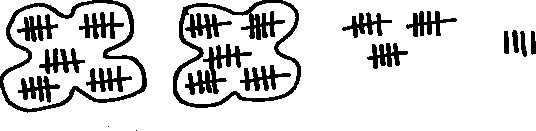
\includegraphics{../graphics/lothar.pdf}
\]
From this picture you discern that Lothar has $69$ goats. Lothar is
studying the tablet intently when his wife, Gertrude, comes in. She
tries in vain to get Lothar to keep track of his goats using another
set of symbols:
\[
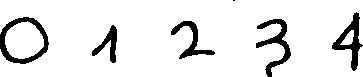
\includegraphics{../graphics/numbers.pdf}
\]
A heated debate between Lothar and Gertrude ensues, the exact details
of which are still a mystery. We do glean the following facts:
\begin{enumerate}
\item Under Gertrude's scheme, five goats are denoted by:
\[

\includegraphics{../graphics/gfive.pdf}
\]
\item The total number of Lothar's goats is denoted by: 
\[
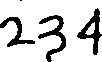
\includegraphics{../graphics/ggoats.pdf}
\]
\end{enumerate}
\begin{question} Can you explain Gertrude's counting scheme?
\end{question}
\QM 

Did I mention that ``your friend's'' time machine is also a spaceship?
Oh\dots Well it is. Now you both travel to the planet Omicron Persei
8.\index{Omicron Persei 8} There are two things you should know about
the inhabitants of Omicron Persei 8:
\begin{enumerate}
\item They only have 3 fingers on each hand.
\item They can eat a human in one bite.
\end{enumerate}
As you can see, there are serious issues that any human visitor to
Omicron Persei 8 must deal with. For one thing, since the Omicronians
only have 3 fingers on each hand, they've only written down the
following symbols for counting:
\[

\includegraphics{../graphics/op8numbers.pdf}
\]
Emperor Lrrr of the Omicronians is tallying how many humans he ate
last week
\[
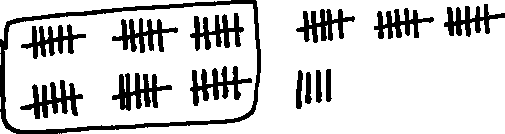
\includegraphics{../graphics/leathuman.pdf}
\]
when his wife, Ndnd, comes in and reminds him that he can write this
number using their fancy symbols as:
\[

\includegraphics{../graphics/op8numbershe.pdf}
\]
After reading some restaurant menus, you find out that twelve
tally-marks are denoted by the symbols:
\[

\includegraphics{../graphics/op8number12.pdf}
\]
\begin{question} Can you explain the Omicronians' counting scheme?
\end{question}
\QM

At this point you hop back into ``your friend's'' space-time
ship. ``Your friend'' kicks off their shoes. You notice that ``your
friend'' has 6 toes on each foot. You strike up a conversation about
the plethora of toes. Apparently this anomaly has enabled ``your
friend'' to create their own counting scheme, which they say is based
on:
\begin{itemize}
\item Toes
\item Feets
\item Feets of Feets
\item and so on\dots
\end{itemize}
``Your friend'' informs you that they would write the number you know
as ``twenty-six'' as $22$ or ``two feets and two toes.'' What?! Though
you find the conversation to be dull and stinky, you also find out
that ``your friend'' uses two more symbols when they count. ``Your
friend'' uses the letter $A$ to mean what you call ``ten,'' and the
letter $B$ to mean what you call ``eleven!''

\begin{question} Can you explain ``your friend's'' counting scheme?
\end{question}
\QM




%\subsection*{Problems for Section \thesection}\hrule\vspace{1ex}
\begin{problems}
\begin{enumerate}
\item Explain why the following ``joke'' is ``funny:'' \textit{There
  are $10$ types of people in the world. Those who understand base $2$
  and those who don't.}
\item You meet some Tripod aliens, they tally by threes. Thankfully
  for everyone involved, they use the symbols $0$, $1$, and $2$. 
\begin{enumerate}
\item Can you explain how a Tripod would count from $11$ to $201$? Be
  sure to carefully explain what number comes after $22$.
\item What number comes immediately before $10$?  $210$? $20110$?
  Explain your reasoning.
\end{enumerate}
\item You meet some people who tally by sevens. They use the symbols
  $O$, $A$, $B$, $C$, $D$, $E$, and $F$. 
\begin{enumerate}
\item What do the individual symbols $O$, $A$, $B$, $C$, $D$, $E$, and
  $F$ mean?
\item Can you explain how they would count from $DD$ to $AOC$? Be sure
  to carefully explain what number comes after $FF$.
\item What number comes immediately before $AO$?  $ABO$? $EOFFA$?
  Explain your reasoning.
\end{enumerate}
\item Now, suppose that you meet a hermit who tallies by
  thirteens. Explain how he might count. Give some relevant and
  revealing examples.
\fixnote{The problem used to begin $1/6$ of $30$ is $4$, but that allowed  
proportional reasoning to give the correct answer.  The numbers have been changed.  
Check that this is better.}
\item While visiting Mos Eisley spaceport, you stop by Chalmun's
  Cantina. After you sit down, you notice that one of the other aliens
  is holding a discussion on fractions. Much to your surprise, they
  explain that $1/6$ of $36$ is $7$. You are unhappy with this,
  knowing that $1/6$ of $36$ is in fact $6$, yet their audience seems
  to agree with it, not you. Next the alien challenges its audience by
  asking, ``What is $1/4$ of $10$?'' What is the correct answer to
  this question, and how many fingers do the aliens have? Explain your
  reasoning.
\item When the first Venusian to visit Earth attended a 6Te grade
  class, it watched the teacher show that
\[
\frac{3}{12} = \frac{1}{4}.
\]
``How strange,'' thought the Venusian. ``On Venus, $\frac{4}{12} =
\frac{1}{4}$.'' What base do Venusians use? Explain your reasoning.
\item When the first Martian to visit Earth attended a high school
  algebra class, it watched the teacher show that the only solution of
  the equation
\[
5x^2-50x+125 = 0
\]
is $x = 5$.

``How strange,'' thought the Martian. ``On Mars, $x = 5$ is a solution
of this equation, but there also is another solution.'' If Martians
have more fingers than humans, how many fingers do Martians have on both hands?
Explain your reasoning.

%\begin{teachingnote}
%Here you cannot factor---you must first convert to base $b$.
%\end{teachingnote}

\item In one of your many space-time adventures, you see the equation
\[
\frac{3}{10} + \frac{4}{13} = \frac{21}{20}
\]
written on a napkin. How many fingers did the beast who wrote this
have? Explain your reasoning.
\item What is the smallest number of weights needed to produce every
  integer-valued mass from $0$ grams to say $n$ grams? Explain your
  reasoning.
\item Starting at zero, how high can you count using just your
  fingers?
\begin{enumerate}
\item Explain how to count to $10$.
\item Explain how to count to $35$.
\item Explain how to count to $1023$.
\item Explain how to count to $59048$.
\item Can you count even higher?
\end{enumerate}
Explain your reasoning.
\end{enumerate}

\end{problems}








\section{Arithmetic}\label{S:aritmetic}

Consider this question:
\begin{activitynote}
Activity \ref{A:HAr} complements this section well.  % Hieroglyphical Arithmetic
\end{activitynote}
\begin{question}
Can you \textit{think} about something if you lack the
\textit{vocabulary} required to discuss it?
\end{question}
\QM

\subsection{Nomenclature}
The numbers and operations we work with have properties whose
importance are so fundamental that we have given them names. Each of
these properties is surely well known to you; however, the importance
of the name is that it gives a keen observer the ability to see and
articulate fundamental structures in arithmetic and algebra.

\paragraph{The Associative Property}\index{associativity} 
An operation \ding{72} is called \textbf{associative} if for all
numbers $a$, $b$, and $c$:
\[
a \,\text{\ding{72}}\, (b \,\text{\ding{72}}\, c) = (a \,\text{\ding{72}}\, b) \,\text{\ding{72}}\, c
\]


\paragraph{The Commutative Property}\index{commutativity}
An operation $\,\text{\ding{72}}\,$ is called \textbf{commutative} if for all
numbers $a$ and $b$:
\[
a \,\text{\ding{72}}\, b = b \,\text{\ding{72}}\, a
\]

\paragraph{The Distributive Property}\index{distributivity}
An operation $\,\text{\ding{72}}\,$ is said to be \textbf{distributive} over another
operation \ding{66} if for all numbers $a$, $b$, and $c$:
\[
a \,\text{\ding{72}}\,(b \,\text{\ding{66}}\, c)  = (a \,\text{\ding{72}}\, b) \,\text{\ding{66}}\, (a\,\text{\ding{72}}\, c)
\qquad\text{and}\qquad (b \,\text{\ding{66}}\, c)\,\text{\ding{72}}\, a  = (b \,\text{\ding{72}}\, a) \,\text{\ding{66}}\, (c\,\text{\ding{72}}\, a)
\]

\paragraph{The Closure Property}\index{closure}
An operation $\,\text{\ding{72}}\,$ is called \textbf{closed} on a set of numbers if for all
numbers $a$ and $b$ in the set:
\[
a \,\text{\ding{72}}\, b \qquad \textrm{is another number in the set}.  
\]


You may find yourself a bit distressed over some of the notation used
above. In particular you surely notice that we were using crazy
symbols like \ding{72} and \ding{66}. We did this for a reason. The
properties above may hold for more than one operation. Let's explore
this:

\begin{question}
Can you give examples of operations that are associative? Can you give
examples of operations that are not associative?
\end{question}
\QM

\begin{question}
Can you give examples of operations that are commutative? Can you give
examples of operations that are not commutative?
\end{question}
\QM


\begin{question}
Can you give examples of two operations where one distributes over the
other? Can you give examples of operations that do not distribute?
\end{question}
\QM


\begin{question}
Can you give examples of an operation and a set of numbers where 
the operation is closed on the set of numbers?  Can you give examples 
of an operation and a set of numbers where 
the operation is not closed on the set of numbers? 
\end{question}
\QM


\subsection{Algorithms}
In elementary school you learned many strategies for addition and subtraction.\standard{2.NBT.9}  
Some of these strategies can be developed into \emph{algorithms}, which are general step-by-step procedures 
for computation.  In this section, we aim to explain various strategies and algorithms for addition and subtraction, and our tools are place value and the properties of operations.\standard{3.NBT.2}
\begin{teachingnote}
Here we seek to have the students acknowledge the algebra behind many
algorithms. We have given a number of examples illustrating the sort
of work we wish to see.
\end{teachingnote}
\begin{activitynote}
Activities \ref{A:B1} and \ref{A:B2} complement  this section well.  % Playing with Blocks & More Playing with Blocks
\end{activitynote}

\paragraph{Standard Addition Algorithm}\index{addition algorithm!standard}
Here is an example of a standard addition algorithm:
\[
\begin{tabular}{@{}r@{}}
11~~\\
892\\
+398\\ \hline
1290
\end{tabular}
\]

\begin{question}
Can you describe how to perform this algorithm?
\end{question}

As a gesture of friendship, I'll take this one. All we are doing here
is adding each column of digits at a time, starting with the right-most
digit
\[
\begin{array}[b]{@{}r@{}}
89\textbf{2}\\
+39\textbf{8}\\ \hline
~~\textbf{10}
\end{array}
\qquad
\leadsto
\qquad
\begin{array}[b]{@{}r@{}}
\textbf{1}~~\\
89\textbf{2}\\
+39\textbf{8}\\ \hline
~~~\textbf{0}
\end{array}
\]
If our column of digits sums to $10$ or higher, then we must ``carry''
the tens-digit of our sum to the next column. This process repeats
until we run out of digits on the left.
\[
\begin{array}[b]{@{}r@{}}
\textbf{1}~~\\
8\textbf{9}2\\
+3\textbf{9}8\\ \hline
~\textbf{19}0
\end{array}
\qquad
\leadsto
\qquad
\begin{array}[b]{@{}r@{}}
\textbf{1}1~~\\
\textbf{8}92\\
+\textbf{3}98\\ \hline
\textbf{12}90
\end{array}
\]
We're done!

\begin{question}
Can you show the ``behind-the-scenes'' algebra going on here?
\end{question}

I'll take this one too. Sure, you just write:
\begin{align*}
892 + 398 &= (8\cdot 10^2 + 9\cdot 10 + 2) + (3 \cdot 10^2 + 9\cdot 10 + 8) \\
&= 8\cdot 10^2 + 9\cdot 10 + 2 + 3 \cdot 10^2 + 9\cdot 10 + 8 \\
&= 8\cdot 10^2 + 3 \cdot 10^2 + 9\cdot 10 + 9\cdot 10 + 2 + 8 \\
&= (8 + 3)\cdot 10^2 + (9 + 9)\cdot 10 + (2 + 8) \\
&= (8 + 3)\cdot 10^2 + (9 + 9)\cdot 10 + 10 + 0\\
&= (8 + 3)\cdot 10^2 + (9 + 9+1)\cdot 10 + 0 \\
&= (8 + 3)\cdot 10^2 + (10 + 9)\cdot 10 + 0 \\
&= (8 + 3+1)\cdot 10^2 + 9\cdot 10 + 0 \\
&= 12\cdot 10^2 + 9\cdot 10 + 0 \\
&= 1290
\end{align*}
Wow! That was a lot of algebra. At each step, you should be able to
explain how to get to the next step, and state which algebraic
properties are being used.


\paragraph{Standard Multiplication Algorithm}\index{multiplication algorithm!standard}
Here is an example of a standard multiplication algorithm:

\[
\begin{array}{@{}r@{}}
23~~\\
634\\
\times~~8\\ \hline
5072
\end{array}
\]

\begin{question}
Can you describe how to perform this algorithm?
\end{question}

Me me me me! All we are doing here is multiplying each digit of the
multi-digit number by the single digit number.
\[
\begin{array}[b]{@{}r@{}}
63\textbf{4}\\
\times~~\textbf{8}\\ \hline
~~\textbf{32}
\end{array}
\qquad
\leadsto
\qquad
\begin{array}[b]{@{}r@{}}
\textbf{3}~~\\
63\textbf{4}\\
\times~~\textbf{8}\\ \hline
~~~\textbf{2}
\end{array}
\]
If our product is $10$ or higher, then we must ``carry'' the
tens-digit of our product to the next column. This ``carried'' number
is then added to our new product. This process repeats until we run
out of digits on the left.
\[
\begin{array}[b]{@{}r@{}}
\textbf{3}~~\\
6\textbf{3}4\\
\times~~\textbf{8}\\ \hline
~\textbf{27}2
\end{array}
\qquad
\leadsto
\qquad
\begin{array}[b]{@{}r@{}}
\textbf{2}3~~\\
\textbf{6}34\\
\times~~\textbf{8}\\ \hline
\textbf{50}72
\end{array}
\]
We're done!

\begin{question}
Can you show the ``behind-the-scenes'' algebra going on here?
\end{question}

You betcha! Just write:
\begin{align*}
634 \cdot 8 &= (6\cdot 10^2 + 3\cdot 10 + 4) \cdot 8\\
&= 6\cdot 8\cdot 10^2 + 3\cdot 8\cdot 10 + 4\cdot 8\\
&= 6\cdot 8\cdot 10^2 + 3\cdot 8\cdot 10 + 32 & &\text{(\ding{95})}\\
&= 6\cdot 8\cdot 10^2 + (3\cdot 8 + 3)\cdot 10  + 2 & &\text{(\ding{96})}\\
&= 6\cdot 8\cdot 10^2 + 270  + 2 & &\text{(\ding{100})}\\
&= (6\cdot 8+2)\cdot 10^2 + 7\cdot 10 + 2& &\text{(\ding{98})}\\
&= 50\cdot 10^2 + 7\cdot 10  + 2\\
&= 5\cdot 10^3 + 0\cdot 10^2 + 7\cdot 10  + 2\\
&= 5072
\end{align*}
Ahhhhh! Algebra works. Remember just as before, at each step you
should be able to explain how to get to the next step, and state which
algebraic properties are being used.

\begin{question} 
Can you clearly explain what happened between lines (\ding{95}) and
(\ding{96})? What about between lines (\ding{100}) and
(\ding{98})?
\end{question}
\QM


\paragraph{Long-Division Algorithm With Remainder}\index{division algorithm!long, with remainder}
\index{long division} Once more we meet with this old foe---long
division.  Here is an example:
\[
8\,\begin{array}[b]{@{}r@{}r} 
97 &\, \text{R}1\\ 
\cline{1-1}
\Big)\begin{array}[t]{@{}l@{}} 777\\ 
72 \\ 
\divrule{0}{2}  ~57 \\
 ~56\\
 \divrule{1}{2}
~~1
\end{array}
\end{array}
\]


\begin{question}
Can you describe how to perform this algorithm?
\end{question}

Yes! I'm all about this sort of thing. All we are doing here is single
digit division for each digit of the multi-digit dividend (the number
under the division symbol) by the single digit divisor (the left-most
number). We start by noting that $8$ won't go into $7$, and so we see
how many times $8$ goes into $77$.
\[
\textbf{8}\,\begin{array}[b]{@{}r@{}} 
\textbf{9}~~\\ 
\hline
\Big)\begin{array}[t]{@{}l@{}} \textbf{77}7\\ 
\textbf{72} \\ 
\divrule{0}{2}  ~\textbf{5} \\
\end{array}
\end{array}
\qquad\leftrightsquigarrow\qquad
\begin{minipage}{7ex}
\begin{align*}%\index{Division Theorem!for integers}
n &= d\cdot q + r \\
77 &= 8\cdot 9 + 5
\end{align*}
\end{minipage}
\]
Now we drop the other $7$ down, and see how many times $8$ goes into
$57$.
\[
\textbf{8}\,\begin{array}[b]{@{}r@{}} 
9\textbf{7}~\\ 
\hline
\Big)\begin{array}[t]{@{}l@{}} 777\\ 
72 \\ 
\divrule{0}{2}  ~\textbf{57} \\
 ~\textbf{56}\\
 \divrule{1}{2}
~~\textbf{1}\\
\end{array}
\end{array}
\qquad\leftrightsquigarrow\qquad
\begin{minipage}{7ex}
\begin{align*}
n &= d\cdot q + r \\
57 &= 8\cdot 7 + 1
\end{align*}
\end{minipage}
\]
This process repeats until we run out of digits in the dividend.

\begin{question}
Can you show the ``behind-the-scenes'' algebra going on here?
\end{question}

Of course---but this time things will be a bit different.
\begin{align*}
77 &= 8\cdot 9 + 5 \\
77\cdot 10 &= (8 \cdot 9  + 5 )\cdot 10 \\
77\cdot 10 &= 8 \cdot 9 \cdot 10 + 5 \cdot 10 \\
77\cdot 10 + 7 &= 8 \cdot 9 \cdot 10 + 5 \cdot 10 + 7 \\
777 &= 8 \cdot (9 \cdot 10) + 57 & &\text{(\ding{95})}\\
777 &= 8 \cdot (9 \cdot 10) + (8\cdot 7 + 1) & &\text{(\ding{96})}\\
777 &= 8 \cdot (9 \cdot 10) + 8\cdot 7 + 1 & &\text{(\ding{100})}\\
777 &= 8 \cdot (9 \cdot 10+7) + 1 & &\text{(\ding{98})}\\
777 &= 8 \cdot 97 + 1 
\end{align*}
Looks good to me, but remember: At each step you must be able to
explain how to get to the next step, and state which algebraic
properties are being used.


\begin{question} 
Can you clearly explain what happened between lines (\ding{95}) and
(\ding{96})? What about between lines (\ding{100}) and (\ding{98})?
\end{question}
\QM





\paragraph{Long-Division Algorithm Without Remainder}
\index{division algorithm!without remainder} 
Do you remember that the division algorithm can be done in such a way
that there is no remainder?  Here is an example of the division
algorithm without remainder:
\[
4\,\begin{array}[b]{@{}l@{}} 
~0.75\\
\hline
\Big)\begin{array}[t]{@{}l@{}}\, 3.00\\ 
\,2\;8 \\ 
\divrule{0}{3}  
~\,\;20 \\
 ~\,\;20\\
 \divrule{1}{3} \vspace{-1.4em} \\ 
 \divrule{1}{3}
\end{array}
\end{array}
\]

\begin{question}
Can you describe how to perform this algorithm?
\end{question}

I'm getting a bit tired, but I think I can do this last one. Again,
all we are doing here is single digit division for each digit of the
multi-digit dividend (the number under the division symbol) by the
single digit divisor (the left-most number) adding zeros after the
decimal point as needed. We start by noting that $4$ won't go into
$3$, and so we see how many times $4$ goes into $3.0$. Mathematically
this is the same question; however, by thinking of the $3.0$ as $30$,
we put ourselves into familiar territory. Since
\[
4 \cdot 7 = 30 \qquad \Rightarrow \qquad 4 \cdot 7 \cdot 10^{-1} = 30
\cdot 10^{-1} = 3
\]
this will work as long as we put our $7$ immediately to the right of
the decimal point.
\[
\textbf{4}\,\begin{array}[b]{@{}l@{}} 
~\textbf{0.7}  \\
\hline
\Big)\begin{array}[t]{@{}l@{}} \textbf{3.0}\\ 
\textbf{2\;8} \\ 
\divrule{0}{3}  
~\;\textbf{2}
\end{array}
\end{array}
\qquad\leftrightsquigarrow\qquad
\begin{minipage}{7ex}%\index{Division Theorem!for integers}
\begin{align*}
n &= d\cdot q + r \\ 30 &= 4\cdot 7 + 2
\end{align*}
\end{minipage}
\]
Now we are left with a remainder of $.2$. To take care of this, we
drop another $0$ down and see how many times $4$ goes into $20$. Since
\[
4 \cdot 5 = 20 \qquad \Rightarrow \qquad 4 \cdot 5 \cdot 10^{-2} = 5
\cdot 10^{-2} = 0.05
\]
this will work as long as we put our $5$ two spaces to the right of
the decimal point.

\[
\textbf{4}\,\begin{array}[b]{@{}l@{}} 
~0.7\textbf{5}\\
\hline
\Big)\begin{array}[t]{@{}l@{}} 3.0\textbf{0}\\ 
2\;8 \\ 
\divrule{0}{3}  ~\textbf{\;20} \\
 ~\;\textbf{20}\\
 \divrule{1}{3} \vspace{-1.4em} \\ 
 \divrule{1}{3}
\end{array}
\end{array}
\qquad\leftrightsquigarrow\qquad
\begin{minipage}{7ex}
\begin{align*}
n &= d\cdot q + r \\
20 &= 4\cdot 5 + 0
\end{align*}
\end{minipage}
\]
This process repeats until we obtain a division with no remainder, or
until we see repetition in the digits of the quotient.

\begin{question}
Can you show the ``behind-the-scenes'' algebra going on here?
\end{question}

Let's do it:
\begin{align*}
3 &= 4\cdot 0 + 3 \\
3.0 &= (4 \cdot 7  + 2 )\cdot 10^{-1} \\
3.0 &= 4 \cdot (7\cdot 10^{-1})  + 2 \cdot 10^{-1} \\
3.00 &= 4 \cdot (7\cdot 10^{-1})  + 20 \cdot 10^{-2} \\
3.00 &= 4 \cdot (7\cdot 10^{-1})  + (4\cdot 5) \cdot 10^{-2} & &\text{(\ding{100})}\\
3.00 &= 4 \cdot (7\cdot 10^{-1})  + 4\cdot (5 \cdot 10^{-2}) & &\text{(\ding{98})}\\
3.00 &= 4 \cdot (7\cdot 10^{-1}  + 5 \cdot 10^{-2}) \\
3.00 &= 4 \cdot 0.75 
\end{align*}
Looks good to me, but remember: At each step you must be able to
explain how to get to the next step, and state which algebraic
properties are being used.


\begin{question} 
Can you clearly explain what happened between lines (\ding{100}) and
(\ding{98})?
\end{question}
\QM








\begin{problems}
\fixnote{Add a problem about the doubling/halving base-two multiplication algorithm....   Perhaps also include the Mysterious base-two game, or make it an activity.}
\begin{enumerate}
\item Explain what it means for an operation \ding{72} to be
  \textit{associative}. Give some relevant and revealing examples and non-examples.
\item \label{P:MA}Consider the following pictures:
\[
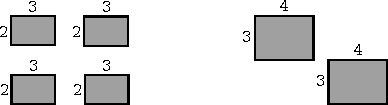
\includegraphics{../graphics/assMult.pdf}
\]
Jesse claims that these pictures represent $(2\cdot 3)\cdot 4$ and
$2\cdot (3\cdot 4)$.
\begin{enumerate}
\item Is Jesse's claim correct? Explain your reasoning.
\item Do Jesse's pictures show the associativity of multiplication? If
  so, explain why. If not, draw new pictures representing $(2\cdot
  3)\cdot 4$ and $2\cdot (3\cdot 4)$ that do show the associativity
  of multiplication.
\end{enumerate}
\item Explain what it means for an operation \ding{72} to be
  \textit{commutative}. Give some relevant and revealing examples  and non-examples.
\item Explain what it means for an operation \ding{72} to \textit{distribute}
  over another operation \ding{66}. Give some relevant and revealing
  examples and non-examples.
\item Explain what it means for an operation \ding{72} to be \textit{closed}
  on a set of numbers. Give some relevant and revealing
  examples and non-examples.
\item Sometimes multiplication is described as \textit{repeated
  addition}. Does this explain why multiplication is commutative? If
  so give the explanation. If not, give another description of
  multiplication that does explain why it is commutative.
\item In a warehouse you obtain $20\%$ discount but you must pay a
  $15\%$ sales tax. Which would save you more money: To have the tax
  calculated first or the discount? Explain your reasoning---be sure
  to use relevant terminology.  In particular, which property 
of which operation(s) do you use?  


\item Money Bags Jon likes to give a tip of $20$\% when he is at
  restaurants. He does this by dividing his bill by $10$ and then
  doubling it. Explain why this works.
\item Regular Reggie likes to give a tip of $15$\% when he is at
  restaurants. He does this by dividing his bill by $10$ and then
  adding half more to this number. Explain why this works.
\item Wacky Wally has a strange way of giving tips when he is at
  restaurants. He does this by rounding his bill up to the nearest
  multiple of $7$ and then taking the quotient (when that new number
  is divided by $7$). Explain why this isn't as wacky as it might
  sound.
%% \begin{teachingnote}
%% The problem above is fundamentally different than the other (related)
%% problems involving tips.
%% \end{teachingnote}

\item Cheap Carl likes to give a tip of $13\frac{1}{3}$\% when he is
  at restaurants. He does this by dividing his bill by $10$ and then
  adding one-third more to this number. Explain why this works.
\item Reasonable Rebbecca likes to give a tip of $18$\% when she is at
  restaurants. She does this by dividing her bill by $5$ and then
  removing one-tenth of this number. Explain why this works.
\item Can you think of and justify any other schemes for computing the
  tip?
\item Here is an example of a standard addition algorithm:
\[
\begin{array}{@{}r@{}}
11~~\\
892\\
+398\\ \hline
1290
\end{array}
\]
\begin{enumerate}
\item Describe how to perform this algorithm.
\item Provide an additional relevant and revealing example
  demonstrating that you understand the algorithm.
\item Show the ``behind-the-scenes'' algebra that is going on here.
\end{enumerate}
\item Here is an example of the column addition
  algorithm:\index{addition algorithm!column}
\[
\begin{array}{@{}r@{}}
892\\
+398\\ \hline
10\\
18~~\\
11~~~\\ \hline
1290
\end{array}
\]
\begin{enumerate}
\item Describe how to perform this algorithm.
\item Provide an additional relevant and revealing example
  demonstrating that you understand the algorithm.
\item Show the ``behind-the-scenes'' algebra that is going on here.
\end{enumerate}

\item If you check out Problems~\ref{P:MS} and \ref{P:DS}, you will
  learn about ``partial'' algorithms.
\begin{enumerate}
\item Develop a ``partial'' algorithm for addition, give it a name, and describe how to
  perform this algorithm.
\item Provide a relevant and revealing example demonstrating that you
  understand the algorithm.
\item Show the ``behind-the-scenes'' algebra that is going on here.
\end{enumerate}
\item Here is an example of the banker's addition
  algorithm:\index{addition algorithm!banker's}
\[
\begin{array}{@{}r@{}}
892\\
+398\\ \hline
1\textbf{0}\\
1\textbf{9}~~\\
\textbf{12}~~~\\ \hline
1290\,
\end{array}
\]
\begin{enumerate}
\item Describe how to perform this algorithm.
\item Provide an additional relevant and revealing example
  demonstrating that you understand the algorithm.
\item Show the ``behind-the-scenes'' algebra that is going on here.
\end{enumerate}
\item Here is an example of a standard subtraction
  algorithm:\index{subtraction algorithm!standard}
\[
\begin{array}{@{}r@{}r@{}r@{}r@{}}
&   & 8 &  \\
& 8 & \not{\hspace{-.2ex}9} & \hspace{.3ex}\leftexp{1}2\\
- & 3 & 7 & 8\\ \hline
& 5 & 1 & 4
\end{array}
\]
\begin{enumerate}
\item Describe how to perform this algorithm.
\item Provide an additional relevant and revealing example
  demonstrating that you understand the algorithm.
\item Show the ``behind-the-scenes'' algebra that is going on here.
\end{enumerate}
\item Here is an example of the subtraction by addition
  algorithm:\index{subtraction algorithm!by addition}
\[
\begin{array}[c]{@{}r@{}}
892\\
-378\\ \hline
514
\end{array} 
\qquad\leftrightsquigarrow\qquad
\begin{minipage}{40ex}
\begin{align*}
8 + \textbf{4} &= 12 & &\text{add $1$ to $7$ to get $8$} \\
8 + \textbf{1} &= 9 \\
3 + \textbf{5} &= 8
\end{align*}
\end{minipage}
\]
\begin{enumerate}
\item Describe how to perform this algorithm.
\item Provide an additional relevant and revealing example
  demonstrating that you understand the algorithm.
\item Show the ``behind-the-scenes'' algebra that is going on here.
\end{enumerate}


\item Here is an example of the Austrian subtraction
  algorithm:\index{subtraction algorithm!Austrian}
\[
\begin{array}{@{}r@{}r@{}r@{}r@{}}
& 8 & 9 & \hspace{.3ex}\leftexp{1}2\\
- & 3 & \hspace{.3ex}\leftexp{8}{\hspace{-.8ex}\not{\hspace{0ex}7}} & 8\\ \hline
& 5 & 1 & 4
\end{array}
\]
\begin{enumerate}
\item Describe how to perform this algorithm.
\item Provide an additional relevant and revealing example
  demonstrating that you understand the algorithm.
\item Show the ``behind-the-scenes'' algebra that is going on here.
\end{enumerate}

\item If you check out Problems~\ref{P:MS} and \ref{P:DS}, you will
  learn about ``partial'' algorithms.
\begin{enumerate}
\item Develop a ``partial'' algorithm for subtraction, give it a name, and describe how to
  perform this algorithm.
\item Provide a relevant and revealing example demonstrating that you
  understand the algorithm.
\item Show the ``behind-the-scenes'' algebra that is going on here.
\end{enumerate}


\item Here is an example of a standard multiplication algorithm:
\[
\begin{array}{@{}r@{}}
23~~\\
634\\
\times~~8\\ \hline
5072
\end{array}
\]
\begin{enumerate}
\item Describe how to perform this algorithm.
\item Provide an additional relevant and revealing example
  demonstrating that you understand the algorithm.
\item Show the ``behind-the-scenes'' algebra that is going on here.
\end{enumerate}
\item\label{P:MS} Here is an example of the partial-products 
  algorithm: \index{multiplication algorithm!partial-products}\index{partial products algorithm}
\[
\begin{array}{@{}r@{}}
634\\
\times~~8\\ \hline
4800\\
240\\
32\\ \hline
5072
\end{array}
\]
\begin{enumerate}
\item Describe how to perform this algorithm.
\item Provide an additional relevant and revealing example
  demonstrating that you understand the algorithm.
\item Show the ``behind-the-scenes'' algebra that is going on here.
\end{enumerate}
\item Here is an example of a standard division algorithm:
\[
8\,\begin{array}[b]{@{}r@{}r} 
97 &\, \text{R}1\\ 
\cline{1-1}
\Big)\begin{array}[t]{@{}l@{}} 777\\ 
72 \\ 
\divrule{0}{2}  ~57 \\
 ~56\\
 \divrule{1}{2}
~~1
\end{array}
\end{array}
\]
\begin{enumerate}
\item Describe how to perform this algorithm.
\item Provide an additional relevant and revealing example
  demonstrating that you understand the algorithm.
\item Show the ``behind-the-scenes'' algebra that is going on here.
\end{enumerate}
\item\label{P:DS} Here is an example of the partial quotients
  algorithm:\index{division algorithm!partial-quotients}
\[
8\,\begin{array}[b]{@{}r@{}} 
7 \\
90\\ 
\hline
\Big)\begin{array}[t]{@{}l@{}} 777\\ 
720 \\ 
\divrule{0}{3}  
~57 \\
 ~56\\
 \divrule{1}{2}
~~1
\end{array}
\end{array}
\]
\begin{enumerate}
\item Describe how to perform this algorithm.
\item Provide an additional relevant and revealing example
  demonstrating that you understand the algorithm.
\item Show the ``behind-the-scenes'' algebra that is going on here.
\end{enumerate}
\item Here is another example of the partial-quotients division
  algorithm:\index{division algorithm!partial-quotients}
\[
8\,\begin{array}[b]{@{}r@{}} 
4\\
10~\\
10~\\
10~\\ 
\hline
\Big)\begin{array}[t]{@{}l@{}} 277\\ 
~80 \\ 
\divrule{0}{3}  
197 \\
~80 \\
\divrule{0}{3}
117 \\
~80 \\
\divrule{0}{3}
~37 \\
~32 \\
\divrule{1}{2}
~~5
\end{array}
\end{array}
\]
\begin{enumerate}
\item Describe how to perform this algorithm---be sure to explain how
  this is different from the scaffolding division algorithm.
\item Provide an additional relevant and revealing example
  demonstrating that you understand the algorithm.
\item Show the ``behind-the-scenes'' algebra that is going on here.
\end{enumerate}
\item Here is an example of a standard multiplication
  algorithm:\index{multiplication algorithm!standard}
\[
\begin{array}{@{}r@{}}
634\\
\times 216\\ \divrule{1}{5}
3804 \\
6340 \\
126800\\ \hline
136944
\end{array}
\]
\begin{enumerate}
\item Describe how to perform this algorithm.
\item Provide an additional relevant and revealing example
  demonstrating that you understand the algorithm.
\item Show the ``behind-the-scenes'' algebra that is going on
  here---you may assume that you already know the algebra behind the 
standard multiplication algorithm.
\end{enumerate}
\item Here is an example of the addition algorithm with decimals:
\[
\begin{array}{@{}r@{}}
1\hspace*{4.2ex}\\
37.2~~\\
+8.74\\ \hline
45.94
\end{array}
\]
\begin{enumerate}
\item Describe how to perform this algorithm.
\item Provide an additional relevant and revealing example
  demonstrating that you understand the algorithm.
\item Show the ``behind-the-scenes'' algebra that is going on here.
\end{enumerate}
\item Here is an example of the multiplication algorithm with
  decimals:
\[
\begin{array}{@{}r@{}}
3.40\\
\times~.21\\ \hline
340\\
6800\\
\hline
.7140
\end{array}
\]
\begin{enumerate}
\item Describe how to perform this algorithm.
\item Provide an additional relevant and revealing example
  demonstrating that you understand the algorithm.
\item Show the ``behind-the-scenes'' algebra that is going on here.
\end{enumerate}
\item Here is an example of the division algorithm without remainder:
\[
4\,\begin{array}[b]{@{}l@{}} 
~0.75\\
\hline
\Big)\begin{array}[t]{@{}l@{}} 3.00\\ 
2\;8 \\ 
\divrule{0}{3}  ~\;20 \\
 ~\;20\\
 \divrule{1}{3} \vspace{-1.4em} \\ 
 \divrule{1}{3}
\end{array}
\end{array}
\]
\begin{enumerate}
\item Describe how to perform this algorithm.
\item Provide an additional relevant and revealing example
  demonstrating that you understand the algorithm.
\item Show the ``behind-the-scenes'' algebra that is going on here.
\end{enumerate}
\item In the following addition problem, every digit has been
  replaced with a letter.
\[
\begin{tabular}{@{}r@{}}
\texttt{MOON}\\
$+$\texttt{ SUN}\\ \hline
\texttt{PLUTO}
\end{tabular}
\]
Recover the original problem and solution. Explain your reasoning.
Hint: $\texttt{S}=6$ and $\texttt{U}=5$.
\item In the following addition problem, every digit has been
  replaced with a letter.
\[
\begin{tabular}{@{}r@{}}
\texttt{SEND}\\
$+$\texttt{MORE}\\ \hline
\texttt{MONEY}
\end{tabular}
\]
Recover the original problem and solution. Explain your reasoning.
\item In the following subtraction problem, every digit has been
  replaced with a letter.
\[
\begin{tabular}{@{}r@{}}
\texttt{DEFER}\\
$-$\texttt{DU7Y}\\ \hline
\texttt{N2G2}
\end{tabular}
\]
Recover the original problem and solution. Explain your reasoning.
\item In the following two subtraction problems, every digit has been
  replaced with a letter.
\[
\begin{tabular}{@{}r@{}}
\texttt{NINE}\\
$-$\texttt{TEN}\\ \hline
\texttt{TWO}
\end{tabular}
\qquad\qquad
\begin{tabular}{@{}r@{}}
\texttt{NINE}\\
$-$\texttt{ONE}\\ \hline
\texttt{ALL}
\end{tabular}
\]
Using both problems simultaneously, recover the original problems and
solutions. Explain your reasoning.
\item In the following multiplication problem, every digit has been
  replaced with a letter.
\[
\begin{tabular}{@{}r@{}}
\texttt{LET}\\
$\times$\texttt{ NO}\\ \hline
\texttt{SOT}\\
\texttt{NOT$~$}\\
\hline
\texttt{FRET}
\end{tabular}
\]
Recover the original problem and solution. Explain your reasoning.

%% \begin{teachingnote}
%% The next two problems may seem tedious, but they are very rewarding
%% for students when they are able to finally solve them. While the
%% student should be encouraged to use a calculator, the solution is not
%% pure ``guess and check'' and there is a lot of reasoning that goes
%% into the solution.
%% \end{teachingnote}

\item The following is a long division problem where every digit
  except 7 was replaced by X.
\settowidth\digitwidth{X}
\def~{\hspace{\digitwidth}}
\[
\text{XX}\,\begin{tabular}[b]{@{}r@{}}
X\,7X \\ \hline
\Big)\begin{tabular}[t]{@{}l@{}}
XXXXX \\
X\,7\,7 \\ \divrule{0}{3}
~X\,7X \\
~X\,7X \\ \divrule{1}{3}
~~~XX\\ 
~~~XX \\ \divrule{3}{2}\vspace{-1.4em} \\ 
 \divrule{3}{2}
\end{tabular}
\end{tabular}
\]
Recover the digits from this long division problem. Explain your
reasoning.
%% \begin{teachingnote}
%% Remind students to use their calculator and that to start,
%% $\mathrm{XX}\cdot \mathrm{X} = \mathrm{X}77$.
%% \end{teachingnote}

\item The following is a long division problem where the various digits were
replaced by X except for a single $8$. The double bar indicates that the remainder is 0.

\[
\text{XXX}\,\begin{tabular}[b]{@{}r@{}}
XX8XX \\ \hline
\Big)\begin{tabular}[t]{@{}l@{}}
XXXXXXXX \\
~XXX \\ \divrule{1}{3}
~~XXXX \\
~~~XXX \\ \divrule{3}{3}
~~~~XXXX\\ 
~~~~XXXX \\ \divrule{4}{4}\vspace{-1.4em} \\ 
 \divrule{4}{4}
\end{tabular}
\end{tabular}
\]
Recover the digits from this long division problem. Explain your
reasoning.

\end{enumerate}
\end{problems}







\section{Algebra}



Algebra is when you replace a number with a letter, usually $x$,
right? OK---but you also do things with $x$, like make
\textit{polynomials} out of it.

\subsection{Polynomial Basics}

\begin{activitynote}
Activity \ref{A:CA} complements this section well.  % Comparative Arithmetic
\end{activitynote}



\begin{question} What's a polynomial? 
\end{question}
\QM

I'll take this one:
\begin{definition}\index{polynomial}
An $n^{th}$-degree \textbf{polynomial} in the variable $x$ is an expression of the form
\[
a_nx^n + a_{n-1}x^{n-1} + \dots + a_1 x + a_0
\]
where the $a_i$'s are all constants, $n$ is a nonnegative integer, and $a_n\neq 0$.
\end{definition}

\begin{question}
Which of the following are polynomials?
\[
3x^3 - 2x + 1 \qquad \frac{1}{3x^3 - 2x + 1} \qquad 3x^{-3} - 2x^{-1} + 1 \qquad 3x^{1/3} - 2x^{1/6} + 1
\]
\end{question}
\QM


Given two polynomials
\begin{align*}
&a_nx^n + a_{n-1}x^{n-1} + \dots + a_1 x + a_0 \\
&b_mx^m + b_{m-1}x^{m-1} + \dots + b_1 x + b_0
\end{align*}
we treat these polynomials much the same way we treat numbers. Note,
an easy fact is that polynomials are equal if and only if their
coefficients are equal---this may come up again!

\begin{question} Are numbers equal if and only if their digits are equal?
\end{question}
\QM

\begin{teachingnote}
This question is foreshadowing a future discussion of real numbers. The
students will probably suggest that it is true---this is OK. We will
address this point later.
\end{teachingnote}

\begin{question} 
Can you explain how to add two polynomials? Compare and contrast this
procedure to the standard addition algorithm for counting numbers.
\end{question}
\QM

\begin{question} 
Can you explain how to multiply two polynomials? Compare and contrast
this procedure to the standard multiplication algorithm for counting numbers.
\end{question}
\QM



\begin{question} 
Can you explain why someone might say that working with polynomials is
like working in ``base $x$?''
\end{question}
\QM


\subsection{Division and Polynomials}

For some reason you keep on signing up for classes with aloof old
Professor Rufus. When he was asked to teach division of polynomials
with remainders, he merely wrote
\[
d(x)\,\begin{tabular}[b]{@{}r@{} r}
$q(x)$ &\, R\,$r(x)$\\ \cline{1-1}
\Big)\begin{tabular}[t]{@{}l@{}}
\bigstrut[t]$n(x)$ 
\end{tabular}
\end{tabular}
\qquad\text{where}\qquad
\begin{tabular}{l}
$d(x)$ is the divisor \\
$n(x)$ is the dividend \\
$q(x)$ is the quotient \\
$r(x)$ is the remainder
\end{tabular}
\]
and walked out of the room, again! Do you have \textit{d\'{e}j\`{a} vu}?

\begin{question} 
Can you give $3$ much needed examples of polynomial long division with
remainders?
\end{question}
\QM

\begin{question} 
Given polynomials $d(x)$, $n(x)$, $q(x)$, and $r(x)$ how do you know
if they leave us with a correct expression above?
\end{question}
\QM


\begin{question} 
Can you explain how to divide two polynomials? 
%Compare and contrast this procedure to the Division Theorem for
%integers.
\end{question}
\QM

\begin{question} 
Can you do the polynomial long division with remainder?
\end{question}
\QM

Again, this question can be turned into a theorem.

\begin{theorem}[Division Theorem]\index{Division Theorem!for polynomials}
Given any polynomial $n(x)$ and a nonconstant polynomial $d(x)$, there exist unique
polynomials $q(x)$ and $r(x)$ such that
\vspace{1in}
\end{theorem}
\noindent The above space has intentionally been left blank for you to
fill in.
\begin{teachingnote}
Here we want the students to realize that
\[
n(x) = d(x)q(x) + r(x)\qquad\text{where } 0 \le \deg(r(x)) < \deg(d(x)) 
\]
\end{teachingnote}




\begin{problems}
\begin{enumerate}
\item Explain what is meant by a \textit{polynomial} in a variable $x$.
\item Given:
\[
3x^7 -x^5 + x^4 -16x^3 + 27 = a_7 x^7 + a_6x^6 + a_5x^5 + a_4x^4 + a_3x^3 + a_2x^2 + a_1x^1 + a_0
\]
Find $a_0$, $a_1$, $a_2$, $a_3$, $a_4$, $a_5$, $a_6$, $a_7$.
\item Given:
\[
6x^5+a_4 x^4 -x^2 + a_0 = a_5 x^5 - 24 x^4 + a_3 x^3 + a_2 x^2 - 5
\]
Find $a_0$, $a_1$, $a_2$, $a_3$, $a_4$, $a_5$.
\item Is it true that polynomials are equal if and only if their
  coefficients are equal? Explain your reasoning.
\item Is it true that numbers are equal if and only if their digits
  are equal? Explain your reasoning.
\item Explain how to add two polynomials. 
\item Explain how to multiply two polynomials.
\item Here is an example of the polynomial division algorithm:
\[
x^2 + 3x + 1\,\begin{tabular}[b]{@{}r@{}r} 
$x-3$~~&\, R\,$9x+4$\\ 
\cline{1-1}
\Big)\begin{tabular}[t]{@{}l@{}} \bigstrut[t] $x^3 + 0x^2 + x + 1$\\ 
$x^3 + 3x^2 + x$ \\ 
\divrule{0}{11}  
\bigstrut[t]~~~$-3x^2 +0x + 1$\\
~~~$-3x^2-9x -3$\\
\divrule{4}{12}
~~~~~~~~~~$9x + 4$
\end{tabular}
\end{tabular}
\]
\begin{enumerate}
\item Describe how to perform this algorithm.
\item Provide an additional relevant and revealing example
  demonstrating that you understand the algorithm.
\item Show the ``behind-the-scenes'' algebra that is going on here.
\end{enumerate}\index{division algorithm!polynomial}
\item State the \textit{Division Theorem} for polynomials. Give some
  relevant and revealing examples of this theorem in action.
\item Given a polynomial
\[
p(x) = a_nx^n + a_{n-1}x^{n-1} + \dots + a_1 x+ a_0
\]
can you find two numbers $L$ and $U$ such that $L \le p(x) \le U$ for
all $x$? If so, explain why. If not, explain why not.
\item Consider all polynomials of the form
\[
a_nx^n + a_{n-1}x^{n-1} + \dots + a_1 x+ a_0
\]
where the $a_i$'s are integers. If you substitute an integer for $x$
will you always get an integer out? Explain your reasoning.
\item Consider the following polynomial:
\[
p(x) = \frac{x^2}{2}+\frac{x}{2}
\]
Will $p(x)$ always returns an integer when an integer is substituted
for $x$? Explain your reasoning.

\item Fix some integer value for $x$ and consider all polynomials of
  the form
\[
a_nx^n + a_{n-1}x^{n-1} + \dots + a_1 x+ a_0
\]
Where the $a_i$'s are integers greater than or equal to $0$. Which
numbers can be represented by such polynomials? Explain your
reasoning.
\item Find a polynomial 
\[
p(x) = a_nx^n + a_{n-1}x^{n-1} + \dots + a_1 x+ a_0
\]
such that $a_i$'s are integers greater than or equal to $0$ and less
than $2$ such that $p(2) = 35$. Discuss how your answer compares to
the representation of $35$ in base $2$. Explain your reasoning.
\item Find a polynomial 
\[
p(x) = a_nx^n + a_{n-1}x^{n-1} + \dots + a_1 x+ a_0
\]
such that $a_i$'s are integers greater than or equal to $0$ and less
than $7$ such that $p(7) = 234$. Discuss how your answer compares to
the representation of $234$ in base $7$. Explain your reasoning. 
\item Find a polynomial 
\[
p(x) = a_nx^n + a_{n-1}x^{n-1} + \dots + a_1 x+ a_0
\]
such that $a_i$'s are integers greater than or equal to $0$ and less
than $10$ such that $p(10) = 18$. Discuss how your answer compares to
the representation of $18$ in base $10$. Explain your reasoning.
\item Find a polynomial 
\[
p(x) = a_nx^n + a_{n-1}x^{n-1} + \dots + a_1 x+ a_0
\]
such that $a_i$'s are integers greater than or equal to $0$ and less
than $15$ such that $p(15) = 201$. Discuss how your answer compares to
the representation of $201$ in base $15$. Explain your reasoning.
\item Fix some integer value for $x$ and consider all polynomials of the form
\[
a_nx^n + a_{n-1}x^{n-1} + \dots + a_1 x+ a_0
\]
Where the $a_i$'s are integers greater than or equal to $0$ and less
than $x$. Which numbers can be represented by such polynomials?
Explain your reasoning. Big hint: Base $x$.
\item Fix some integer value for $x$ and consider all polynomials of
  the form
\[
a_nx^n + a_{n-1}x^{n-1} + \dots + a_1 x+ a_0
\]
Where the $a_i$'s are integers greater than or equal to $0$ and less
than $10$. Which numbers can be represented by such polynomials?
Explain your reasoning.

\item Consider $x^2 + x + 1$. This can be thought of as a ``number'' in
  base $x$. Express this number in base $(x+1)$, that is, find $b_0$, $b_1$, $b_2$ such that 
\[
b_2(x+1)^2 +b_1(x+1) + b_0 = x^2 + x + 1.
\]
Explain your reasoning.

\item Consider $x^2 + 2x + 3$. This can be thought of as a ``number'' in
  base $x$. Express this number in base $(x-1)$, that is, find $b_0$, $b_1$, $b_2$ such that 
\[
b_2(x-1)^2 +b_1(x-1) + b_0 = x^2 + 2x + 3.
\]
Explain your reasoning.

\item Consider $x^3 + 2x + 1$. This can be thought of as a ``number'' in
  base $x$. Express this number in base $(x-1)$, that is, find $b_0$, $b_1$, $b_2,$ $b_3$ such that 
\[
b_3(x-1)^3 + b_2(x-1)^2 +b_1(x-1) + b_0 = x^3 + 2x + 1.
\]
Explain your reasoning.

\item If the polynomial
\[
p(x) = a_nx^n + a_{n-1}x^{n-1} + \cdots + a_1x + a_0
\]
is thought of as a ``number'' in base $x$, describe two different ways
to find the base $(x-1)$ coefficients of $p(x)$.

\end{enumerate}
\end{problems}





\chapter{Numbers}

\begin{quote}
God created the integers, the rest is the work of man.

\hfill---Leopold Kronecker 
\end{quote}

\section{The Integers}
An important theme in this course is distinguishing among the various number systems of school mathematics.  A \emph{number system} is a set of numbers together with arithmetic operations, such as addition and multiplication, on those numbers.  We have already been using \textit{counting numbers}.  Now we need to be more precise.  

\begin{teachingnote}
A theme in this chapter and throughout the course is ``general reasoning with specific numbers.''
\end{teachingnote}

\begin{definition}\index{integers}\index{Z@$\Z$}
The \textbf{counting numbers}, often called the \textbf{natural numbers}, are (naturally) those use for counting.  We use the symbol $\N$ to denote the counting numbers:  
\[
\N = \{1, 2, 3, 4, 5, \dots\}
\]

When $0$ is included with the counting numbers, we have the set of \textbf{whole numbers}, denoted $\W$:  
\[
\W = \{0, 1, 2, 3, 4, 5, \dots\}
\]

The set of counting numbers, zero, and negative counting numbers is called
the set of \textbf{integers}, denoted $\Z$:
\[
\Z = \{\dots, -5,-4,-3,-2,-1,0,1,2,3,4,5,\dots \}
\]
\end{definition}

In case you're wondering, the symbol $\Z$ is used because
\textit{Zahlen} is the German word for ``numbers.'' 

\subsection{Addition}
\begin{teachingnote}
Key meanings of addition are ``adding to'' and ``putting together.''
\end{teachingnote}

Addition is probably the first operation we learn.    

\begin{question}
Write a story problem whose solution is given by the expression
$19+17$. Let this context be a ``working model'' for addition.
\end{question}
\QM

\begin{question}
Does your model show associativity of addition? If so, explain how. If
not, can you come up with a new model (story problem) that does?
\end{question}
\QM

\begin{question}
Does your model show commutativity of addition? If so, explain how. If
not, can you come up with a new model that does?
\end{question}
\QM

An observant reader might notice that we have thus far given no reason to have 
negative integers.  

\begin{question}
Describe some contexts (story problems) in which negative numbers are useful.  
It will help to think of contexts in which there are ``opposite'' numbers in some sense.  
\end{question}
\QM

\begin{question}
Does your addition model work with negative integers?  In other words, does it model 
$19+ (-17)$ and $8 + (-13)$?  If so, explain how. If not, can you modify your model or 
come up with a new model that does work?
\end{question}
\QM

\subsection{Subtraction}
\begin{question}
Write a story problem whose solution is given by the expression
$19-17$. Let this context be a ``working'' model for subtraction.  
\end{question}
\QM

\begin{question}
We know that 
\[
a - b  = a + (-b),
\]
but the left-hand side of the equation is conceptually
different from the right-hand side of the equation. Write two story
problems, one solved by $19-17$ and the other solved by
$19+(-17)$. What's the difference? (Pun intended!)
\end{question}
\QM

\begin{teachingnote}
Here we are trying to have the students develop the ``take-away,''
along with the ``missing addend,'' and a ``comparison'' model for
subtraction.
\end{teachingnote}


\begin{question}
Can you use the two story problems above to model
\[
(-19)-17, \qquad  19 - (-17), \qquad (-19) - (-17)?
\]
\end{question}
\QM

\begin{question}
How is \emph{subtraction} different from \emph{negation}?  
\end{question}
\QM

\subsection{Multiplication}
Multiplication is more multifaceted than addition. 

\begin{question}
Write a story problem whose solution is given by the expression
$19\cdot 17$. Let this context be a ``working'' model for multiplication. 
\end{question}
\QM

\begin{teachingnote}
We would like to point out that the units used in addition are generally
the same for the different summands. However, with multiplication, the
different factors often have different units.
\end{teachingnote}

\begin{question}
Does your model show commutativity of multiplication? If so, explain
how. If not, can you come up with a new model that does?
\end{question}
\QM

\begin{question}
Does your model show associativity of multiplication? If so, explain
how. If not, can you come up with a new model that does?
\end{question}
\QM

\begin{teachingnote}
This question is with Problem~\ref{P:MA} of
Section~\ref{S:aritmetic} in mind. In particular to show
associativity, we suggest appealing to the notion of volume.
\end{teachingnote}


\begin{question}
Does your model work with negative integers? In particular does your
model show that
\[
\text{positive}\cdot \text{negative} = \text{negative},
\]
\[
\text{negative}\cdot \text{positive} = \text{negative},
\]
and 
\[
\text{negative}\cdot \text{negative} = \text{positive}?
\]
If so, explain how. If not, can you come up with a new model that
does?
\end{question}
\QM

\begin{teachingnote}
This is difficult. The students may not be able to come up with a
model that works. This is OK---as this issue is addressed in
Problem~\ref{P:NNP}.
\end{teachingnote}


\subsection{Division} 

While addition and multiplication are good operations, the real
``meat'' of the situation comes with division.

\begin{definition}\index{divides}    %\index{dn@$d "| n$} %% the pipe breaks stuff
We say that a non-zero integer $d$ \textbf{divides} an integer $n$ if there is
an integer $q$ such that 
\[
n = dq.
\]
In this case we write $d \mid n$, which is said: ``$d$ divides $n$.''  If $d$ does not divide $n$, 
we sometimes write $d \nmid n$.  
\end{definition}

While this may seem easy, it is actually quite tricky. You must always
remember the following synonyms for \textit{divides}:
\[\index{multiple}\index{factor}
\text{``$d$ \textbf{divides} $n$''}\leftrightsquigarrow 
\text{``$d$ is a \textbf{divisor} of $n$''}\leftrightsquigarrow
\text{``$d$ is  a \textbf{factor} of $n$''}\leftrightsquigarrow 
\text{``$n$ is a  \textbf{multiple} of $d$''}
\]

\begin{activitynote}
Activity \ref{A:dm} complements this section well.  % What Can Division Mean
\end{activitynote}

\begin{definition}\index{prime number} 
A \textbf{prime} number is a positive integer with exactly two
positive divisors, namely $1$ and itself.
\end{definition}

\begin{definition}\index{composite number} 
A \textbf{composite} number is a positive integer with more than two
positive divisors.
\end{definition}

I claim that every composite number is divisible by a prime number. Do
you believe me? If not, consider this:
\begin{quote}
Suppose there was a composite number that was \textit{not} divisible
by a prime. Then there would necessarily be a \textit{smallest}
composite number that is not divisible by a prime. Since this number
is composite, this number is the product of two even smaller numbers,
both of which have prime divisors. Hence our original number must have
prime divisors.
\end{quote}
\begin{question} 
What the heck just happened?! Can you rewrite the above paragraph,
drawing pictures and/or using symbols as necessary, making it more
clear?
\end{question}
\QM


\begin{activitynote}
Activity \ref{A:Pr} complements this section well.  %  There's Always Another Prime
\end{activitynote}


\subsection{Factoring}

At this point we can factor any composite completely into primes. To
do this, it is often convenient to make a \textit{factor
  tree}:\index{factor tree}

\[
\xymatrix@R=0pt@C=10pt{
  & 360 \ar@{-}[dl] \ar@{-}[dr] & & & & &\\
2 &     & 180 \ar@{-}[dl] \ar@{-}[dr] & & & & \\ 
  &  2   &     & 90 \ar@{-}[dl] \ar@{-}[dr] & & & \\
  &      &  2  &    & 45  \ar@{-}[dl] \ar@{-}[dr] & & \\ 
  &      &     & 5  &    & 9 \ar@{-}[dl] \ar@{-}[dr] &\\ 
  &      &     &    &  3  &  & 3
}
\]

From this tree\footnote{Why is this a tree? It looks more like roots to me!} we see that
\[
360 = 2^3 \cdot 3^2 \cdot 5.
\]

At each step we simply divided by whichever prime number seemed most
obvious, branched off the tree and kept on going. From our factor
tree, we can see some of the divisors of the integer in
question. However, there are many composite factors that can be built
up from the prime divisors. One of the most important is the
\textit{greatest common divisor}.

\begin{definition}\index{GCD}\index{greatest common divisor} 
The \textbf{greatest common divisor} (GCD) of two integers $a$ and $b$ (not both 0)
is a positive integer $g = \gcd(a,b)$ where:
\begin{enumerate}
\item $g|a$ and $g|b$.
\item If $d|a$ and $d|b$, then $0 < d \le g$.
\end{enumerate}
\end{definition}

\begin{question}
Describe informally what the greatest common divisor of two numbers means.  
Explain how the two conditions in the formal definition appear in your informal description. 
\end{question}
\QM

\begin{question}
What can you conclude when $\gcd(a,b)=1$?  Explain. 
\end{question}
\QM

\begin{question}
How can you use a factor tree to compute the GCD of two integers?
\end{question}
\QM

\begin{question}
Describe informally what the least common multiple (LCM)\index{LCM}\index{least common multiple} 
of two numbers means.  Write a formal definition of LCM.  Explain how the two conditions in the formal 
definition appear in your informal description. 
\end{question}
\QM

\begin{question}
How can you use a factor tree to compute the LCM of two integers?
\end{question}
\QM


So, to factor an integer or find the GCD, one could use a factor
tree. However, when building the factor tree, we had to know what
primes to divide by. What if no prime comes to mind? What if you want
to factor the integer $391$ or $397$? This raises a new question:

\begin{question} 
How do you check to see if a given integer is prime? What possible
divisors must you check? When can you stop checking?
\end{question}
\QM


\begin{activitynote}
Activities \ref{A:Hall} and \ref{A:Sieve} complements this section well. % Hall of Shoes and Sieving It All Out
\end{activitynote}


%\begin{question}
%How should you identify all the primes between $1$ and $100$? Big
%hint: Maybe you should either go to the shoe store, or read up on
%Eratosthenes.\index{Eratosthenes}
%\end{question}
%\QM







\subsection{Division with Remainder}


We all remember long division\index{long division}, or at least we
remember \textit{doing} long division. Sometimes, we need to be
reminded of our \textit{forgotten foes}\index{forgotten foes}. When
aloof old Professor Rufus was trying to explain division to his class,
he merely wrote
\[
d\,\begin{tabular}[b]{@{}r@{} r}
$q$ &\, R\,$r$\\ \cline{1-1}
\big)\begin{tabular}[t]{@{}l@{}}
$n$ 
\end{tabular}
\end{tabular}
\qquad\text{where}\qquad
\begin{tabular}{l}
$d$ is the divisor \\ \index{divisor}
$n$ is the dividend \\ \index{dividend}
$q$ is the quotient \\ \index{quotient}
$r$ is the remainder \index{remainder}
\end{tabular}
\]
and walked out of the room.

\begin{question} 
Can you give $3$ much needed examples of long division with
remainders?
\end{question}
\QM

\begin{question} 
Given positive integers $d$, $n$, $q$, and $r$ how do you know if they
leave us with a correct expression above?
\end{question}
\QM

\begin{question} 
Given positive integers $d$ and $n$, how many different sets of $q$
and $r$ can you find that will leave us with a correct expression
above?
\end{question}
\QM


The innocuous questions above can be turned into a theorem. We'll start
it for you, but you must finish it off yourself:

\begin{theorem}[Division Theorem]\index{Division Theorem!for integers}
Given any integer $n$ and a nonzero integer $d$, there exist unique
integers $q$ and $r$ such that
\vspace{1in}
\end{theorem}
\noindent The above space has intentionally been left blank for you to
fill in.


\begin{teachingnote}
Here we want the students to realize that
\[
n = dq + r\qquad\text{where } 0 \le r < d 
\]
\end{teachingnote}


Now consider the following picture:
\[
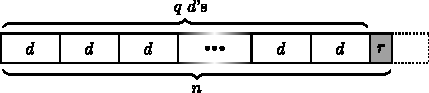
\includegraphics{../graphics/divisionThmProof.pdf}
\]
\begin{question} 
How does the picture above ``prove'' the Division Theorem for positive
integers? How must we change the picture if we allow negative values
for $n$ and $d$?
\end{question}
\QM

\begin{teachingnote}
Highlight uniqueness:  The requirement that  $0 \le r < d$ makes both $d$ and $r$ unique.  Without that requirement, 
many $d$ and $r$ pairs will work.  

The second part of this question is quite challenging.  Some specific examples can help.  
\end{teachingnote}




\begin{activitynote}
Activity \ref{A:CF} complements this section well.  % There Are Many Factors to Consider
\end{activitynote}


\newpage


\begin{problems}
\begin{enumerate}
\item Describe the set of integers. Give some relevant and revealing
  examples/nonexamples.
\item Explain how to model integer addition with pictures or
  items. What relevant properties should your model show?
\item Explain how to model integer multiplication with pictures or
  items. What relevant properties should your model show?
\item Explain what it means for one integer to \textit{divide} another
  integer. Give some relevant and revealing examples/nonexamples.
\item Use the definition of \textit{divides} to decide whether the
  following statements are true or false. In each case, an explanation must 
be given justifying your claim.
\begin{enumerate}
\item $5|30$
\item $7|41$
\item $0|3$
\item $3|0$
\item $6|(2^2\cdot 3^4\cdot 5 \cdot 7)$
\item $1000|(2^7\cdot 3^9\cdot 5^{11}\cdot 17^8)$
\item $6000|(2^{21}\cdot 3^{17}\cdot 5^{89}\cdot 29^{20})$
\end{enumerate}
\item \textit{Incognito's Hall of Shoes} is a shoe store that just
  opened in Myrtle Beach, South Carolina. At the moment, they have 100
  pairs of shoes in stock. At their grand opening 100 customers showed
  up. The first customer tried on every pair of shoes, the second
  customer tried on every 2nd pair, the third customer tried on every
  3rd pair, and so on until the 100th customer, who only tried on the
  last pair of shoes.
\begin{enumerate}
\item Which shoes were tried on by only 1 customer?
\item Which shoes were tried on by exactly 2 customers?
\item Which shoes were tried on by exactly 3 customers?
\item Which shoes were tried on by the most number of customers?
\end{enumerate}
Explain your reasoning.
\item Factor the following integers:
\begin{enumerate}
\item $111$
\item $1234$
\item $2345$
\item $4567$
\item $111111$
\end{enumerate}
In each case, how large a prime must you check before you can be sure
of your answers? Explain your reasoning.
\item Which of the following numbers are prime?  Explain how could deduce whether the numbers are prime in
  as few calculations as possible:
\[
29 \qquad 53 \qquad 101 \qquad 359 \qquad 779 \qquad 839 \qquad 841
\]
In each case, describe precisely which computations are needed and
why those are the only computations needed.
\item Suppose you were only allowed to perform at most $7$
  computations to see if a number is prime. How large a number could
  you check?  Explain your reasoning.
\item Find examples of integers $a$, $b$, and $c$ such that $a \mid
  bc$ but $a\nmid b$ and $a\nmid c$. Explain your reasoning.
\item Can you find at least $5$ composite integers in a row? What
  about at least $6$ composite integers? Can you find $7$?
  What about $n$?  Explain your reasoning. Hint: Consider something
  like $5! = 5\cdot 4 \cdot 3 \cdot 2 \cdot 1$.
\item Use the definition of the \textit{greatest common divisor} to
  find the GCD of each of the pairs below. In each
  case, a detailed argument and explanation must be given justifying
  your claim.
\begin{enumerate}
\item $\gcd(462,1463)$
\item $\gcd(541,4669)$ 
\item $\gcd(10000,2^5\cdot 3^{19}\cdot 5^7\cdot 11^{13})$
\item $\gcd(11111,2^{14}\cdot 7^{21}\cdot 41^{5}\cdot 101)$
\item $\gcd(437^5,8993^3)$
\end{enumerate}

\item Lisa wants to make a new quilt out of $2$ of her favorite
  sheets. To do this, she is going to cut each sheet into as large
  squares as possible while using the entire sheet and using whole
  inch measurements. 
\begin{enumerate}
\item If the first sheet is $72$ inches by $60$ inches what size
  squares should she cut? 
\item If the second sheet is $80$ inches by $75$ inches, what size
  squares should she cut? 
\item How she might sew these squares together? 
\end{enumerate}
Explain your reasoning.
\item Deena and Doug like to feed birds. They want to put 16 cups of
  millet seed and 24 cups of sunflower seeds in their feeder.
\begin{enumerate}
\item How many total scoops of seed (millet or sunflower) are required
  if their scoop holds 1 cup of seed?
\item How many total scoops of seed (millet or sunflower) are required
  if their scoop holds 2 cups of seed?
\item How large should the scoop be if we want to minimize the total
  number of scoops?
\end{enumerate}
Explain your reasoning.
\item Consider the expression:
\[
d\,\begin{tabular}[b]{@{}r@{} r}
$q$ &\, R\,$r$\\ \cline{1-1}
\big)\begin{tabular}[t]{@{}l@{}}
$n$ 
\end{tabular}
\end{tabular}
\qquad\text{where}\qquad
\begin{tabular}{l}
$d$ is the divisor \\
$n$ is the dividend \\
$q$ is the quotient \\
$r$ is the remainder
\end{tabular}
\]
\begin{enumerate}
\item Give $3$ relevant and revealing examples of long division with
  remainders.
\item Given positive integers $d$, $n$, $q$, and $r$ how do you know
  if they leave us with a correct expression above?
\item Given positive integers $d$ and $n$, how many different sets of
  $q$ and $r$ can you find that will leave us with a correct
  expression above?
\item Give $3$ relevant and revealing examples of long division with
  remainders where some of $d$, $n$, $q$, and $r$ are negative.
\item Still allowing some of $d$, $n$, $q$, and $r$ to be negative,
  how do we know if they leave us with a correct expression above?
\end{enumerate}
\item State the \textit{Division Theorem} for integers. Give some
  relevant and revealing examples of this theorem in action.
\item Explain what it means for an integer to \textit{not} divide
  another integer. That is, explain symbolically what it should mean
  to write:
\[
a \nmid b
\]
\item Consider the following:
\begin{align*}
20 \div 8 &= 2 \text{ remainder }4, \\
28 \div 12 &= 2 \text{ remainder }4.
\end{align*}
Is it correct to say that $20 \div 8 = 28 \div 12$? Explain your reasoning.
%\item Explain how if 
%\[
%n = dq_0 + r_0
%\]
%and $r_0> d$, you can find new $q$ and $r$ such that $n = dq+r$ and
%$0\le r< d$.
\item Give a formula for the $n$th even number. Show-off your formula
  with some examples.
\item Give a formula for the $n$th odd number. Show-off your formula
  with some examples.
\item Give a formula for the $n$th multiple of $3$. Show-off your
  formula with some examples.
\item Give a formula for the $n$th multiple of $-7$. Show-off your
  formula with some examples.
\item Give a formula for the $n$th number whose remainder when divided
  by $5$ is $1$. Show-off your formula
  with some examples.

\item Explain the rule
\[
\text{even} + \text{even} = \text{even}
\]
in two different ways. First give an explanation based on
pictures. Second give an explanation based on algebra. Your
explanations must be general, not based on specific examples.
\item Explain the rule
\[
\text{odd} + \text{even} = \text{odd}
\]
in two different ways. First give an explanation based on
pictures. Second give an explanation based on algebra.  Your
explanations must be general, not based on specific examples.
\item Explain the rule
\[
\text{odd} + \text{odd} = \text{even}
\]
in two different ways. First give an explanation based on
pictures. Second give an explanation based on algebra. Your
explanations must be general, not based on specific examples.
\item Explain the rule
\[
\text{even} \cdot \text{even} = \text{even}
\]
in two different ways. First give an explanation based on
pictures. Second give an explanation based on algebra. Your
explanations must be general, not based on specific examples.
\item Explain the rule
\[
\text{odd} \cdot \text{odd} = \text{odd}
\]
in two different ways. First give an explanation based on
pictures. Second give an explanation based on algebra. Your
explanations must be general, not based on specific examples.
\item Explain the rule
\[
\text{odd} \cdot \text{even} = \text{even}
\]
in two different ways. First give an explanation based on
pictures. Second give an explanation based on algebra. Your
explanations must be general, not based on specific examples.
\item Let $a\ge b$ be positive integers with $\gcd(a,b) =1$. Compute
  $\gcd(a +b, a-b)$. Explain your reasoning. Hints: 
\begin{enumerate}
\item Make a chart.
\item If $g|x$ and $g|y$ explain why $g|(x+y)$.
\end{enumerate}
\item Make a chart listing all pairs of positive integers whose
  product is $18$. Do the same for $221$, $462$, and $924$. Use this
  experience to help you explain why when factoring a number $n$, you
  only need to check factors less than or equal to $\sqrt{n}$.
\item \label{P:NNP}Matt is a member of the Ohio State University
  Marching Band. Being rather capable, Matt can take $x$ steps of size
  $y$ inches for all integer values of $x$ and $y$.  If $x$ is
  positive it means \textit{face North and take $x$ steps.} If $x$ is
  negative it means \textit{face South and take $|x|$ steps.} If $y$
  is positive it means your step is a \textit{forward step of $y$
    inches.} If $y$ is negative it means your step \textit{is a
    backward step of $|y|$ inches.}
    \fixnote{We need additional models, e.g., checks and bills, red and black chips. 
    Some of these are incorporated into Activities \ref{A:integerAddition} and \ref{A:integerMultiplication}}
\begin{enumerate}
\item Discuss what the expressions $x \cdot y$ means in this
  context. In particular, what happens if $x = 1$? What if $y=1$?
\item Using the context above, write and solve a word problem that
  demonstrates the rule:
\[
\text{negative}\cdot \text{positive} = \text{negative}
\]
Clearly explain how your problem shows this.
\item Using the context above, write and solve a word problem that
  demonstrates the rule:
\[
\text{negative}\cdot \text{negative} = \text{positive}
\]
Clearly explain how your problem shows this.
\end{enumerate}
\item Stewie decided to count the pennies he had in his piggy bank. He
  decided it would be quicker to count by fives. However, he ended
  with two uncounted pennies. So he tried counting by twos but ended
  up with one uncounted penny. Next he counted by threes and then by
  fours, each time there was one uncounted penny. Though he knew he
  had less than a dollars worth of pennies, and more than 50 cents, he
  still didn't have an exact count. Can you help Stewie out? Explain
  your reasoning.
\end{enumerate}
\end{problems}





\section{The Fundamental Theorem of Arithmetic}\index{Fundamental Theorem!of arithmetic}\label{S:FT}
In the previous section, we found divisors, greatest common divisors, and prime factors of positive integers.  And when we
 found prime factorizations of integers, we used factor trees to organize our work.  

\begin{question}
Jake and Jenna use factor trees to find prime factorizations of the same large number.  Assuming that they don't make any mistakes will their prime factorizations be the same or could they be different?  Explain.  
\end{question}
\QM

Let's try a simpler question. 

\begin{question} If $11 | 50a$, is it true that $11|a$?  Explain and generalize.  
\end{question}
\QM


The following \textit{lemma}\index{lemma} will help us tie these 
ideas together.  What is a lemma, you
ask? A lemma is nothing but a little theorem that helps us solve
another problem.

%Note that a lemma should not be confused with the
%more sour \index{lemon|see{lemma}}\textit{lemon}, as that is something
%different and unrelated to what we are discussing.

\begin{lemma}[Euclid's Lemma]\index{Euclid's Lemma} 
If $p$ is a prime number and $a$ and $b$ are integers
\[
p|ab \qquad\text{implies that} \qquad p | a\text{ or } p|b.
\]
\end{lemma}

We are going to assume Euclid's Lemma without proof (at least for now) because we want to use 
it to prove our fundamental theorem---sometimes called the \textit{Fundamental Theorem of Arithmetic}:

\begin{activitynote}
Activity \ref{A:Prome} complements this section well.  % Prome Factorization
\end{activitynote}

\begin{theorem}[Unique Factorization]\index{Unique Factorization Theorem}\index{Fundamental Theorem!of Arithmetic}
Every integer greater than 1 can be factored uniquely (up to ordering)
into primes.
\end{theorem}

\begin{proof}
Well, if an integer is prime, we are done. If an integer is composite,
then it is divisible by a prime number. Divide and repeat with the
quotient. If our original integer was $n$, we'll eventually get:
\[
n = p_1p_2 \cdots p_m
\]
where some of the $p_i$'s may be duplicates. 

How do we know this factorization is unique? Well, suppose that
\[
n = p_1p_2 \cdots p_m = q_1q_2\cdots q_l
\]
where the $p_i$'s and the $q_j$'s are all prime. By the
definition of ``divides''
\[
p_1 |q_1(q_2\cdots q_l).
\]
So by Euclid's Lemma, $p_1$ must divide either $q_1$ or $(q_2\cdots q_l)$. 
If $p_1 \nmid q_1$, then 
\[
p_1 |q_2(q_3\cdots q_l).
\]
Repeat this
enough times and you will find that $p_1 | q_j$ for one of the $q_j$'s
above, which implies that $p_1 = q_j$. Repeat this process for all 
the $p_i$'s and you see that the factorization is unique.
\end{proof}

\begin{question} 
Huh?! Can you explain what just happened drawing pictures and/or using
symbols as necessary? How do we know the process will terminate?  
Once we see that $p_i | q_j$ for some $j$, how do we know that $p_i = q_j$?
Could you also give some examples?
\end{question}
\QM

\begin{question} 
Thinking about Unique Factorization of the Integers, explain why it
makes sense to exclude $1$ from the prime numbers.
\end{question}
\QM


\begin{question} 
Thinking about Unique Factorization of the Integers, what must be the
case when a number in base ten has units digit of $0$?  What about in other bases?  
\end{question}
\QM

From high school algebra, you have lots of tools for solving equations.  
But in some situations, we are interested only in whole number or integer solutions 
to these equations.  These kinds of equations have a special name:  

\begin{definition}\index{Diophantine equation}
A \textbf{Diophantine equation} is an equation where only integer
solutions are deemed acceptable.
\end{definition}

In this section, we are particularly interested solve \textit{linear Diophantine equations}, that is, equations of the form:
\[
ax + by = c
\]
where $a$, $b$, and $c$ are integers and the only solutions we will
accept are pairs of integers $x$ and $y$.  


\newpage

\begin{problems}

\begin{enumerate}
\item Explain what the GCD of two integers is. Give some relevant and
  revealing examples/nonexamples.
\item Explain what the LCM of two integers is. Give some relevant and
  revealing examples/nonexamples.
\item Consider the Diophantine equation:
\[
15x + 4y = 1
\]
\begin{enumerate}
\item Find a solution to this equation. Explain your reasoning.
\item Compute the slope of the line $15x + 4y = 1$ and write it in
  lowest terms. Show your work.
\item Plot the line determined by $15x + 4y = 1$ on graph paper.
\item Using your plot and the slope of the line, explain how to find
  $10$ more solutions to the Diophantine equation above.
\end{enumerate}
\item Explain why a Diophantine equation 
\[
ax + by = c
\]
has either an infinite number of solutions or zero solutions.
\item Josh owns a box containing beetles and spiders. At the moment,
  there are $46$ legs in the box. How may beetles and spiders are
  currently in the box? Explain your reasoning.
\item How many different ways can thirty coins (nickles, dimes, and
  quarters) be worth five dollars? Explain your reasoning.
\item Lisa collects lizards, beetles and worms. She has more worms
  than lizards and beetles together. Altogether in the collection
  there are twelve heads and twenty-six legs. How many lizards does
  Lisa have?  Explain your reasoning.
\item Can you make exactly \$$5$ with exactly $100$ coins assuming you
  can only use pennies, dimes, and quarters? If so how, if not why
  not?  Explain your reasoning.
\item A merchant purchases a number of horses and bulls for the sum
  of $1770$ talers. He pays $31$ talers for each bull, and $21$ talers
  for each horse. How many bulls and how many horses does the merchant
  buy? Solve this problem, explain what a \textit{taler} is, and
  explain your reasoning---note this problem is an old problem by
  L.\ Euler, it was written in the $1700$'s.
\item A certain person buys hogs, goats, and sheep, totaling $100$
  animals, for $100$ crowns; the hogs cost him $3\frac{1}{2}$ crowns
  a piece, the goats $1\frac{1}{3}$ crowns, and the sheep go for
  $\frac{1}{2}$ crown a piece. How many did this person buy of each?
  Explain your reasoning---note this problem is an old problem from
  \textit{Elements of Algebra} by L.\ Euler, it was written in the
  $1700$'s.
\item How many zeros are at the end of the following numbers:
\begin{enumerate}
\item $2^2 \cdot 5^8 \cdot 7^3\cdot 11^5$
\item $11!$
\item $27!$
\item $99!$
\item $1001!$
\end{enumerate}
In each case, explain your reasoning.
\item Decide whether the following statements are true or false. In
  each case, a detailed argument and explanation must be given
  justifying your claim.
\begin{enumerate}
\item $7|56$
\item $55|11$
\item $3|40$
\item $100 | (2^4\cdot 3^{17} \cdot 5^2\cdot 7)$
\item $5555 | (5^{20}\cdot 7^9\cdot 11^{11}\cdot 13^{23})$ 
\item $3| (3+ 6 + 9 + \cdots +300 + 303)$
\end{enumerate}
\item Suppose that 
\[
(3^5 \cdot 7^9 \cdot 11^x \cdot 13^y) | (3^a \cdot 7^b \cdot 11^{19} \cdot 13^7)
\]
What values of $a$, $b$, $x$ and $y$, make true statements? Explain
your reasoning.
\item Decide whether the following statements are true or false. In
  each case, a detailed argument and explanation must be given
  justifying your claim.
\begin{enumerate}
\item If $7|13a$, then $7|a$.
\item If $6|49a$, then $6|a$. 
\item If $10|65a$, then $10|a$.
\item If $14|22a$, then $14|a$.
\item $54|931^{21}$.
\item $54|810^{33}$.
\end{enumerate}
\item Joanna thinks she can see if a number is divisible by 24 by
  checking to see if it's divisible by 4 and divisible by 6.  She
  claims that if the number is divisible by 4 and by 6, then it must
  be divisible by 24.

Lindsay has a similar divisibility test for 24: She claims that if a
number is divisible by 3 and by 8, then it must be divisible by 24.

Are either correct?  Explain your reasoning.
\item Generalize the problem above.
\item Suppose that you have a huge bag of tickets. On each of the
  tickets is one of the following numbers. 
\[
\{6, 18, 21, 33, 45, 51, 57, 60, 69, 84\}
\]
Could you ever choose some combination of tickets (you can use as many
copies of the same ticket as needed) so that the numbers sum to 7429?
If so, give the correct combination of tickets. If not explain why
not.
\item\label{P:helper} Decide whether the following statements are true
  or false. In each case, a detailed argument and explanation must be
  given justifying your claim.
\begin{enumerate}
\item If $a^2|b^2$, then $a|b$.
\item If $a|b^2$, then $a|b$.
\item If $a|b$ and $\gcd(a,b) = 1$, then $a = 1$.
\end{enumerate}
\item Betsy is factoring the number $24949501$. To do this, she
  divides by successively larger primes. She finds the smallest prime
  divisor to be $499$ with quotient $49999$. At this point she
  stops. Why doesn't she continue? Explain your reasoning.
\item When Ann is half as old as Mary will be when Mary is three times
  as old as Mary is now, Mary will be five times as old as Ann is
  now. Neither Ann nor Mary may vote. How old is Ann? Explain your
  reasoning.
\item If $x^2 = 11\cdot y$, what can you say about $y$? Explain your
  reasoning.
\item If $x^2 = 25\cdot y$, what can you say about $y$? Explain your
  reasoning.
\item When asked how many people were staying at the \textit{Hotel
  Chevalier}, the clerk responded ``The number you seek is the
  smallest positive integer such that dividing by $2$ yields a perfect
  square, and dividing by $3$ yields a perfect cube.'' How many people
  are staying at the hotel? Explain your reasoning.
\end{enumerate}
\end{problems}

\newpage 


\section{The Euclidean Algorithm}\index{Euclidean algorithm}\label{S:EA}
In section~\ref{S:FT}, we assumed Euclid's Lemma and used it to prove the Fundamental 
Theorem of Arithmetic (aka Unique Factorization).  In this section, we backtrack 
to prove Euclid's Lemma.  

\begin{question}
What was Euclid's Lemma?
\end{question}
\QM

\begin{teachingnote}
An important point of this section is to make the student think about
the distributive property. One should try to point out each time
\[
a(x+y) = ax + ay
\]
occurs.
\end{teachingnote}

Up to this point, computing the GCD of two integers required you to
factor both numbers.  This can be difficult to do. The following
algorithm, called the \textit{Euclidean algorithm}, makes finding
GCD's quite easy. With that said, algorithms can be tricky to
explain. Let's try this---study the following calculations, they are
examples of the Euclidean algorithm in action:
\begin{align*}
22 &= \boldsymbol{6}\cdot 3 + \boldsymbol{4}\\ 
\boldsymbol{6} &= \boldsymbol{4}
\cdot 1 + \fbox{$\boldsymbol{2}$}\\ 4 &= 2 \cdot 2 + 0 \qquad 
\fbox{$\therefore \gcd(22,6) = 2$}
\end{align*}

\begin{align*}
33 &= \boldsymbol{24}\cdot 1 + \boldsymbol{9}\\
\boldsymbol{24} &= \boldsymbol{9} \cdot 2 + \boldsymbol{6}\\
\boldsymbol{9} &= \boldsymbol{6} \cdot 1 + \fbox{$\boldsymbol{3}$}\\
6 &= 3 \cdot 2 + 0 \qquad \fbox{$\therefore \gcd(33,24) = 3$} 
\end{align*}

\begin{align*}
42 &= \boldsymbol{16}\cdot 2 + \boldsymbol{10}\\
\boldsymbol{16} &= \boldsymbol{10} \cdot 1 + \boldsymbol{6}\\
\boldsymbol{10} &= \boldsymbol{6} \cdot 1 + \boldsymbol{4}\\
\boldsymbol{6} &= \boldsymbol{4} \cdot 1 + \fbox{$\boldsymbol{2}$}\\
4 &= 2 \cdot 2 + 0 \qquad \fbox{$\therefore \gcd(42,16) = 2$} 
\end{align*}

\begin{question}
Can you describe how to do the Euclidean algorithm?
\end{question}
\QM

\begin{question}
Can you explain why the Euclidean algorithm will always stop? Hint:
Division Theorem.
\end{question}
\QM


\begin{activitynote}
Activity \ref{A:GCDwork} complements this section well.  % Why Does It Work? 
\end{activitynote}


The algorithm demonstrated above is called the \textit{Euclidean
  algorithm} or \textit{Euclid's algorithm} because
Euclid\index{Euclid} uses it several times in Books VII and X of his
book \textit{The Elements}. Donald Knuth\index{Knuth} gives a
description of the Euclidean algorithm in the first volume of his
series of books \textit{The Art of Computer Programming}. Given
integers $m$ and $n$, he describes it as follows:
\begin{quote}
\begin{enumerate} 
\item\label{A:E1} [Find remainder.] Divide $m$ by $n$ and let $r$ be the remainder. (We will have $0\le r< n$.)
\item{[Is it zero?]} If $r=0$, the algorithm terminates; $n$ is the answer.
\item{[Interchange.]} Set $m \leftarrow n$, $n \leftarrow r$, and go
  back to step \ref{A:E1}.
\end{enumerate}
\end{quote}

\begin{question}
What do you think of this description? How does it compare to your
description of the Euclidean algorithm?
\end{question}
\QM

While the Euclidean algorithm is handy and fun, its real power is that
it helps us solve equations. Specifically it helps us solve 
linear Diophantine equations.

Let's study the following calculations:

\begin{tabular}{lr}
\begin{minipage}{15em}
{\begin{align*}
22 &= 6\cdot 3 + 4 &\Leftrightarrow & &  22-6\cdot 3 &= \boldsymbol{4}\\ 
6 &= 4\cdot 1 + 2 &\Leftrightarrow  & &  6 - \boldsymbol{4}\cdot 1 &= 2\\ 
4 &= 2 \cdot 2 + 0 
\end{align*}}
\end{minipage}
&
\begin{minipage}{15em}
{\begin{align*}
6 - 4\cdot 1 &= 2 \\
6 - (22-6\cdot 3)\cdot 1 &= 2 \\
6\cdot 4 + 22(-1) &= 2 
\end{align*}}
\end{minipage} \\
\multicolumn{2}{c}{\fbox{$\therefore 22x + 6y =2$ where $x = -1$ and $y = 4$}}
\end{tabular}

\begin{tabular}{lr}
\begin{minipage}{15em}
{\begin{align*}
33 &= 24\cdot 1 + 9 & \Leftrightarrow & & 33 - 24\cdot 1 &= \boldsymbol{9}\\
24 &= 9 \cdot 2 + 6 & \Leftrightarrow & & 24 - \boldsymbol{9}\cdot 2 &= \boldsymbol{6}\\
9 &= 6 \cdot 1 + 3 & \Leftrightarrow & & 9 - \boldsymbol{6} \cdot 1  &= 3\\
6 &= 3 \cdot 2 + 0  
\end{align*}}
\end{minipage}
&
\begin{minipage}{15em}
{\begin{align*}
9 - 6 \cdot 1  &= 3 \\
9 - (24 - 9\cdot 2) \cdot 1  &= 3 \\
9\cdot 3 +  24\cdot(-1)  &= 3 \\
(33 - 24\cdot 1)\cdot 3 +  24\cdot(-1)  &= 3 \\
33\cdot 3 + 24\cdot (-4) &=3
\end{align*}}
\end{minipage} \\
\multicolumn{2}{c}{\fbox{$\therefore 33x + 24y =3$ where $x = 3$ and $y = -4$}}
\end{tabular}


\begin{question} 
Can you explain how to solve Diophantine equations of the form
\[
ax + by = g
\]
where $g = \gcd(a,b)$?
\end{question}
\QM



The Euclidean algorithm is also useful for theoretical
questions.

\begin{question} 
Given integers $a$ and $b$, what is the smallest positive integer that
can be expressed as
\[
ax + by
\]
where $x$ and $y$ are also integers?
\end{question}

\fixnote{This argument could be improved, as could the corresponding activity, \ref{A:GCDwork}.}

I'm feeling chatty, so I'll take this one. I claim that $g =
\gcd(a,b)$ is the smallest positive integer that can be
expressed as
\[
ax + by
\]
where $x$ and $y$ are integers. How do I know? Well first, the Euclidean algorithm shows that $g$ can be 
expressed as a sum $ax + by$.  (Why?)  

Second, suppose there was
a smaller positive integer, say $s$ where:
\[
ax + by = s
\]
Hmmm\dots but we know that $g|a$ and $g|b$. This means that $g$
divides the left-hand-side of the equation. This means that $g$
divides the right-hand-side of the equation. So $g|s$---but this is
impossible, as $s< g$. Thus $g$ is the smallest integer that can be
expressed as $ax +by$.


\begin{question} Can you now use the Euclidean Algorithm to prove Euclid's Lemma?
\end{question}
\QM


\newpage
\begin{problems}
\begin{enumerate}
\item Explain what a \textit{Diophantine equation} is. Give an example
  and explain why such a thing has real-world applications.
\item Use the Euclidean algorithm to find: $\gcd(671,715)$,
  $\gcd(667,713)$, $\gcd(671,713)$, $\gcd(682,715)$, $\gcd(601,735)$,
  and $\gcd(701,835)$.
\item Explain the advantages of using the Euclidean algorithm to find
  the GCD of two integers over factoring.
\item Find integers $x$ and $y$ satisfying the following Diophantine
  equations:
\begin{enumerate}
\item $671x + 715 y = 11$ 
\item $667x + 713 y = 69$ 
\item $671x + 713 y = 1$
\item $682x + 715 y = 55$
\item $601x + 735 y = 4$
\item $701x + 835 y = 15$
\end{enumerate}
\item Given integers $a$, $b$, and $c$, explain how you know when a
  solution to a Diophantine equation of the form
\[
ax + by = c
\]
exists.
\item Consider the Diophantine equation:
\[
15x + 4y = 1
\]
\begin{enumerate}
\item Use the Euclidean Algorithm to find a solution to this
  equation. Explain your reasoning.
\item Compute the slope of the line $15x + 4y = 1$ and write it in
  lowest terms. Show your work.
\item Plot the line determined by $15x + 4y = 1$ on graph paper.
\item Using your plot and the slope of the line, explain how to find
  $10$ more solutions to the Diophantine equation above.
\end{enumerate}
\item Explain why a Diophantine equation 
\[
ax + by = c
\]
has either an infinite number of solutions or zero solutions.
\end{enumerate}
\end{problems}



\newpage
\section{Rational Numbers}

Once you are familiar with integers, you start to notice something:
Given an integer, it may or may not divide into another integer
evenly. This property is at the heart of our notions of factoring and
primality. Life would be very different if all nonzero integers
divided evenly into one another. With this in mind, we introduce
\textit{rational numbers}.  
\begin{activitynote}
Activities \ref{A:EF} and \ref{A:FO} complement this section well.  
% Picture Models for Equivalent Fractions & Picture Models for Fraction Operations
\end{activitynote}



\begin{definition} 
A \textbf{rational number}\index{rational numbers} can be written as $\dfrac{a}{b}$ where $a\in\Z$, $b\in\Z$, and $b\ne 0$.
\end{definition}

In other words, rational numbers can be written as a fraction of integers, where the denominator is nonzero.
\begin{warning}
Note the words ``can be'' in the definition.  Rational numbers do not have to be represented as fractions.  And fractions are not necessarily rational numbers.  
\end{warning}

\begin{question}
Which of the following numbers are rational?
$$\frac{5}{4}, \qquad 718, \qquad \sqrt{2}, \qquad 2.718, \qquad \frac{22}{7}, \qquad \frac{12}{4}, \qquad \frac{\pi}{3}, \qquad \frac{\sqrt{2}}{\sqrt{8}}, \qquad \frac{1}{43}$$
\end{question}

The set of all \textbf{rational numbers} is denoted by the symbol $\Q$: 
\[
      \Q = \left\{\frac{a}{b}\text{ such that $a\in\Z$ and $b\in\Z$ with $b\ne 0$}\right\}\index{Q@$\Q$}\index{e@$\in$}
\]
The letter $\Q$ stands for the word \textit{quotient}, which should remind us of
fractions.   The funny little ``$\in$'' symbol means ``is in'' or ``is an element of.'' Fancy folks will replace the words \textit{such that} with a colon
``:'' to get:
\[
 \Q = \left\{\frac{a}{b}:\text{$a\in\Z$ and $b\in\Z$ with $b\ne 0$}\right\}
\]


\subsection{Why do People Hate Fractions?}

Why do so many people find fractions difficult? This is a question
worth exploring. We'll guide you through some of the tough spots with
some questions of our own.

\begin{question}
Given a rational number $\dfrac{a}{b}$, come up with three other different rational numbers
that are all equal to $\dfrac{a}{b}$. What features of fractions are we
illustrating?
\end{question}
\QM

\begin{question}
Given two positive rational numbers $\dfrac{a}{b}$ and $\dfrac{c}{d}$, explain how to tell which is greater. What features of fractions are we illustrating?
\end{question}
\QM

\begin{question} 
Given two rational numbers $\dfrac{a}{b}$ and $\dfrac{c}{d}$ with $\dfrac{a}{b} < \dfrac{c}{d}$, explain how one
might find a rational number between them. What features of fractions are we
illustrating?
\end{question}
\QM


\begin{question} 
Dream up counting numbers $a$, $b$, and $c$ such that:
\[
\frac{a/b}{c} = \frac{a}{b/c}
\]
Can you dream up other counting numbers $a'$, $b'$, and $c'$ such that:
\[
\frac{a'/b'}{c'} \neq \frac{a'}{b'/c'}
\]
What features of fractions are we illustrating?
\end{question}
\QM

\begin{question}
Explain how to add two fractions $\dfrac{a}{b}$ and $\dfrac{c}{d}$. What features of
fractions are we illustrating?
\end{question}
\QM


\begin{question} 
Can you come up with any other reasons fractions are difficult?
\end{question}
\QM

\begin{teachingnote}
Two key points of this dialog are: 
\begin{enumerate}
\item Equal fractions have different representations. 
\item It is difficult to compare fractions. 
\end{enumerate}
\end{teachingnote}




\subsection{Basic Meanings of Fractions}
\begin{activitynote}
Activities \ref{A:FlourPower} through \ref{A:CrossSomething} complement this section well. 
%% Flour Power, Picture Yourself Dividing, Cross Something-ing
\end{activitynote}
Like all numbers, fractions have meanings outside of their pure
mathematical existence. Let's see if we can get to the heart of some
of this meaning.\standard{3.NF.1}
\begin{question}
Draw a rectangle. Can you shade $3/8$ of this rectangle? Explain the
steps you took to do this.
\end{question}
\QM


\begin{question}
Draw a rectangle. Given a fraction $a/b$ where $0< a\le b$, explain how
to shade $a/b$ of this rectangle.
\end{question}
\QM


\begin{question}
Draw a rectangle. How could you visualize $8/3$ of this rectangle?
Explain the steps you took to do this.
\end{question}
\QM


\begin{question}
Draw a rectangle. Given a fraction $a/b$ where $0< b< a$, explain how
to visualize $a/b$ of this rectangle.
\end{question}
\QM

\begin{question}
Draw a rectangle.  Can you shade
\[
\frac{3/8}{4}
\]
of this rectangle? Explain the steps you took to do this.
\end{question}
\QM



\newpage

\begin{problems}
\begin{enumerate}
\item Describe the set of rational numbers. Give some relevant and
  revealing examples/nonexamples.
\item What algebraic properties do the rational numbers enjoy that the
  integers do not? Explain your reasoning.
\item What number gives the same result when added to $1/2$ as when
  multiplied by $1/2$. Explain your reasoning.
\item Draw a rectangle to represent a garden. Shade in $3/5$ of the
  garden. Without changing the shading, show why $3/5$ of the garden
  is the same as $12/20$ of the garden. Explain your reasoning.
\item Shade in $2/3$ of the entire picture below:
\[
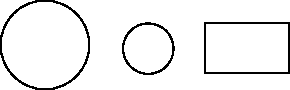
\includegraphics{../graphics/fracPart.pdf}
\]
Explain your reasoning.
\item What fractions could the following picture be illustrating?
\[

\includegraphics{../graphics/whichFrac.pdf}
\]
Explain your reasoning.
\item When Jesse was asked what the $7$ in the fraction $\frac{3}{7}$
  means, Jesse said that the ``$7$'' is the \textit{whole}. Explain
  why this is not completely correct. What is a better description of
  what the ``$7$'' in the fraction $\frac{3}{7}$ means?

\item Find yourself a sheet of paper. Now, suppose that this sheet of
  paper is actually $4/5$ of some imaginary larger sheet of
  paper. 
\begin{itemize}
\item Shade your sheet of paper so that $3/5$ of the larger
  (imaginary) sheet of paper is shaded in. Explain why your shading is
  correct.
\item Explain how this shows that 
\[
\frac{3/5}{4/5} = \frac{3}{4}.
\]
\end{itemize}
\item Try to find the largest rational number smaller than $3/7$.
  Explain your solution or explain why this cannot be done.
\item How many rational numbers are there between $3/4$ and $4/7$?
  Find $3$ of them. Explain your reasoning. 
\item A youthful Bart loved to eat hamburgers. He ate $5/8$ pounds of
  hamburger meat a day. After testing revealed that his blood
  consisted mostly of cholesterol, Bart decided to alter his eating
  habits by cutting his hamburger consumption by $3/4$. How many
  pounds of hamburger a day did Bart eat on his new
  ``low-cholesterol'' diet?  Explain your reasoning.
\item Courtney and Paolo are eating popcorn. Unfortunately, $1/3$rd 
  of the popcorn kernels are poisoned. If Courtney eats exactly $5/16$th 
  of the kernels and Paolo eats exactly $5/13$ths of the kernels, did at 
  least one of them eat a poisoned kernel?  Explain your reasoning.  Also, 
  at least how many kernels of popcorn are in the bowl? Again, explain 
  your reasoning.
\item Best of clocks, how much of the day is past if there remains
  twice two-thirds of what is gone? Explain what this strange question
  is asking and answer the question being sure to explain your
  reasoning---note this is an old problem from the \textit{Greek
    Anthology} compiled by Metrodorus around the year 500.
\item John spent a fifth of his life as a boy growing up, another
  one-sixth of his life in college, one-half of his life as a bookie,
  and has spent the last six years in prison. How old is John now?
  Explain your reasoning
\item Diophantus was a boy for $1/6$th of his life, his beard grew
  after $1/12$ more, he married after $1/7$th more, and a son was born
  five years after his marriage. Alas! After attaining the measure of
  half his father's full life, chill fate took the child. Diophantus
  spent the last four years of his life consoling his grief through
  mathematics. How old was Diophantus when he died?  Explain your
  reasoning---note this is an old problem from the \textit{Greek
    Anthology} compiled by Metrodorus around the year 500.
\item Wandering around my home town (perhaps trying to find my former
  self!), I suddenly realized that I had been in my job for
  one-quarter of my life. Perhaps the melancholia was getting the best
  of me, but I wondered: How long would it be until I had been in my
  job for one-third of my life? Explain your reasoning.
\item In a certain adult condominium complex, $2/3$ of the men are
  married to $3/5$ of the women. Assuming that men are only married to
  women (and vice versa), and that married residents' spouses are also
  residents, what portion of the residents are married? 
\begin{enumerate}
\item Before any computations are done, use common sense to guess the
  solution to this problem.
\item Try to get a feel for this problem by choosing numbers for the
  unknowns and doing some calculations. What do these calculations say
  about your guess?
\item Use algebra to solve the problem.
\end{enumerate}
Explain your reasoning in each step above.

\item Let $a$, $b$, $c$, and $d$ be positive integers such that 
\[
a<b<c<d
\]
Is it true that 
\[
\frac{a}{b}<\frac{c}{d}?
\]
Explain your reasoning.
\item\label{P:CF1} Let $a$, $b$, $c$, and $d$ be positive consecutive
  integers such that
\[
a<b<c<d.
\]
Is it true that 
\[
\frac{a}{b}<\frac{c}{d}?
\]
Explain your reasoning.
\item\label{P:CF2} Let $a$, $b$, $c$, and $d$ be positive consecutive
  integers such that
\[
a<b<c<d.
\]
Is it true that 
\[
\frac{a}{b}<\frac{b}{c}<\frac{c}{d}?
\]
Explain your reasoning.
\item Can you generalize Problem \ref{P:CF1} and Problem \ref{P:CF2}
  above? Explain your reasoning.
\item Let $a$, $b$, $c$, and $d$ be positive integers such that 
\[
\frac{a}{b}<\frac{c}{d}.
\]
Is it true that 
\[
\frac{a}{a+b}<\frac{c}{c+d}?
\]
Explain your reasoning.
\end{enumerate}
\end{problems}

\section{Decimal Representations}

There are two ways that we usually write real numbers that aren't whole numbers:  as fractions and as decimals.  Let's explore the relationship between these two representations of numbers.  

\begin{activitynote}
Activities \ref{A:hundredthsGrids}, \ref{A:Shampoo}, and \ref{A:DecNotNice} are intended for this section. 
% Hundredths Grid
% Shampoo Rinse Repeat
% Decimals Aren't So Nice
\end{activitynote}

\begin{question} How is a ``fraction'' different from a rational number?  
\end{question}
\QM

First, let's work on translating fraction representations into decimal representations.  You probably already know from school that some numbers have decimal representations that end (these are called ``terminating'' decimals) and the rest of them have decimal representations that never end (these are ``non-terminating'').  Try to figure out what it would take for a fraction to have a terminating decimal representation.  

\begin{question}
Write $.465$, $0.72895$, $0.00673$, and $34.062$ as fractions of integers.  What do you notice about terminating decimals when they are written as fractions?  
\end{question}
\QM

\begin{question}
Write $4/5$, $7/16$, $43/20$, and $3/6250$ as decimals.   What about these fractions makes the decimals terminate?
\end{question}
\QM

\begin{question}
Your calculator is not trustworthy for determining whether a number's decimal representation terminates or repeats.  Why?  How can you use your calculator carefully to judge whether a decimal terminates or repeats?  
\end{question}
\QM

In Activity \ref{A:Shampoo}, you separate a bunch of fractions according to whether they appear to have a terminating or non-terminating decimals.  The rational numbers that have a terminating decimals are straighforward to describe, once you see the idea.  The real action (and the intrigue) lies with the non-terminating ones.  

Let's investigate with a fraction that has a non-terminating representation:  4/7.  As you know, 4/7 is the same as ``4 divided by 7.''  So, use long division to find the decimal representation.\standard{7.NS.2d}Bring a pillow, because you already know that it will take an infinite number of steps to complete the work!

Now that you've spent your life doing long division, can you carefully explain why the fraction's non-terminating representation will ``repeat''?  (Hint:  Think about remainders.)  Try a few others, like 2/13, 3/11, or 4/17.  Will the same sort of thing happen with, say, 3457/213678940753?  What can you say about how soon the process will repeat?  

Here are some cool things you can investigate on the side:
\begin{itemize}
\item Some non-terminating decimals have a ``delay'' before they start repeating.  (The most famous one is probably $1/6$.)  I happen to know 1/123750000 will have a delay of 7 places before the repeating starts.  Can you look at a fraction and predict whether it will or will not have a delay (and how long that delay will be)?   
\item What are the restrictions to the sizes of the ``blocks'' for the repeating decimal representation of a rational number?  For example, any fraction with denominator 37 can only possibly repeat in blocks of 1, 2, 3, 4, 6, 9, 12, 18, or 36.
\end{itemize}

Based on the ideas you have explored, you can prove that a non-terminating decimal representation of a rational number must repeat.  Is the converse true?  Can any repeating decimal be written as a fraction?  It turns out indeed to be the case, as can be found by taking advantage of a nice pattern involving the decimals representations of 1/9, 1/99, 1/999, etc., or by noting that each repeating decimal is a ``geometric series,'' as we will explore later.  

Thus, we have it that every rational number can be written as either a terminating or repeating decimal.\standard{8.NS.1}  Can every decimal be written as a fraction?  That is, we have that all fractions are decimals, but are all decimals fractions?  Have we let any decimals out in the cold here?

\begin{question} Describe the decimal representations of 3 ``homemade'' decimals that could never be written as fractions of integers.  Explain your thinking.  Warning:  Do \emph{not} say  $\sqrt{2}$, $\pi$, $e$, or the like, unless you are ready to convince the class that these are not rational numbers.
\end{question}
\QM

\subsection{A Note on Infinite Processes}
Mathematical reasoning often involves ``infinite processes'' in which direct calculation is impossible.\margincomment{This discussion draws heavily on ideas described in \emph{Where Mathematics Comes  From: How the embodied mind brings mathematics into being}  by Lakoff and N\'{u}\~{n}ez (2000).}  Infinite processes become central in calculus, where both differentiation and integration are defined via limits.  These approaches are made rigorous in advanced undergraduate courses, such as Real Analysis.  But infinite processes arise from time to time even in middle grades mathematics, and so it is important that teachers are able to talk about them sensibly and accurately.  Here we explain some key ideas for reasoning about infinite processes.  

First, there is the idea of a process that continues, over and over, without end.  
Here are some examples:
\begin{quote}
\begin{itemize}
\item Perhaps the earliest of these is counting: 1, 2, 3, 4, \dots.  We do not imagine completing the process of counting.  Nonetheless, for any large positive number you name, we can imagine exceeding that number, eventually, if we have enough time.  
\item We can approximate $1/3$ with a sequence, $0.3$, $0.33$, $0.333$, and so on.  We can get as close to $1/3$ as we like by including enough digits.  Note, on the other hand, that it is false to say that $0.3333 = 1/3$ or even $0.3333333333 = 1/3$, because any finite number of digits will miss $1/3$ by an amount that can be calculated precisely.  
\item If we look at a sequence of regular $n$-gons of the same diameter, as $n$ gets large, we can get as close to a circle as we might like.  But for any finite number of sides, the regular $n$-gon will not actually be a circle.  
\end{itemize}
\end{quote}

The above examples use what is sometimes called \emph{potential infinity}, for in none of the cases do we actually complete the process, and we do not need to.  We imagine these things as going on ``forever,'' and a process that goes on forever never ends.  

But the interesting uses of infinity in mathematics involve \emph{actual infinity}.  
\begin{question}
In each of the above examples, what would happen if the process could end?
\end{question}
\QM

In order to conceptualize actual infinity, we imagine, metaphorically, that the process \emph{does} end.  In a literal sense, an infinite process cannot end, but through the use of metaphor, we consider what would happen if the process were to end.  And with the help of intuitions about completed processes, we then infer the ``ultimate result'' of the completed infinite process.    

With the metaphor of actual infinity, counting yields the infinite set of counting numbers, $\N$.  All of them.  In the repeating decimal for $1/3$, we get an exact decimal representation, so that $0.33333\ldots = 1/3$.  Exactly.  And in the case of the regular $n$-gon with an infinite number of sides, we get a circle.  Perfectly.  

\begin{warning}
With the metaphor of actual infinity, it is \emph{false} to say that $0.3333\ldots$ never gets to $1/3$ because the dots imply that the infinite process has been completed.  Although any finite number of digits fails reach $1/3$, an infinite number of digits reaches $1/3$ exactly:  The error has gone to 0.  
\end{warning}

In summary, reasoning about infinite processes involves the following steps:  
\begin{quote}
\begin{enumerate}
\item Describing the finite process carefully and accurately;
\item Considering the process to go on forever, and describing how the result can get arbitrarily close to some goal;
\item Imagining that the infinite process has been completed; and
\item Reasoning about the ``ultimate result'' of the infinite process.
\end{enumerate}
\end{quote}

For some infinite processes, it is quite helpful in the second and fourth steps to talk about the ``error,'' which is to say how much the finite process falls short of the ultimate goal, and then to argue that the error becomes arbitrarily small (i.e., it goes to 0). 

\vspace{0.2in}

Happy infinite reasoning!   

\newpage

\begin{problems}
\begin{enumerate}

\subsection*{Exercises}

\item What does $3.417$ mean in the base-ten place-value system?  Using the rectangle below as $1$, draw a picture the illustrates the place-value meaning of $3.417$.  Draw as accurately as you can, indicating how the picture would be drawn perfectly (if you could).  Indicate whether your model is primarily about length, area, or something else.  

\vspace{.5cm}
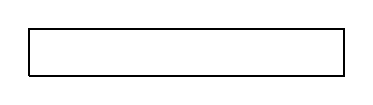
\begin{tikzpicture}
\draw [thick] (0,0) -- (4,0) -- (4,.6) -- (0,.6) -- (0,0);
\end{tikzpicture}

\item Plot $3.417$ on each of the following number lines, zooming in to show how to make the placement more accurate at each step.  Draw dotted curves (as shown) to indicate where the zooming takes place, and label the large tick marks on each number line.  
\vspace{0.5cm}

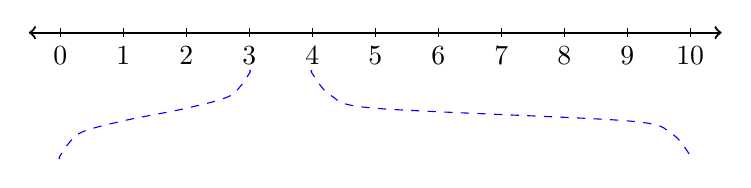
\begin{tikzpicture}[scale=0.8]
% a straight line segment
\draw [thick, <->] (-0.5,0) -- (10.5,0);
% the ticks and their labels
\foreach \x  in {0,...,10}
  \draw[xshift=\x cm] (0pt,2pt) -- (0pt,-2pt) node[below,fill=white] {\the\numexpr\x \relax};

\draw[dashed, blue] plot [smooth] coordinates{(3,-0.6) (3,-0.65) (2.7,-1) (2,-1.2) (1,-1.4)  (0.3,-1.6) (0,-1.95) (0,-2)};
\draw[dashed, blue] plot [smooth] coordinates{(4,-0.6) (4,-0.65) (4.3,-1) (5,-1.2) (9,-1.4)  (9.7,-1.6) (10,-1.95) (10,-2)};
\end{tikzpicture}

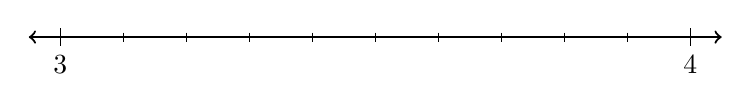
\begin{tikzpicture}[scale=0.8]
% a straight line segment
\draw [thick, <->] (-0.5,0) -- (10.5,0);
% the ticks and their labels
 \draw[xshift=0 cm] (0pt,4pt) -- (0pt,-4pt) node[below,fill=white] {\the\numexpr3 \relax};
\foreach \x  in {1,...,9}
  \draw[xshift=\x cm] (0pt,2pt) -- (0pt,-2pt);
 \draw[xshift=10 cm] (0pt,4pt) -- (0pt,-4pt) node[below,fill=white] {\the\numexpr4 \relax};
\end{tikzpicture}

\vspace{0.8cm}

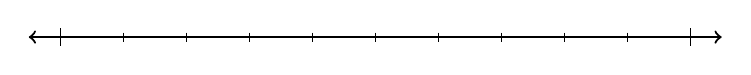
\begin{tikzpicture}[scale=0.8]
% a straight line segment
\draw [thick, <->] (-0.5,0) -- (10.5,0);
% the ticks and their labels
 \draw[xshift=0 cm] (0pt,4pt) -- (0pt,-4pt) ; 
\foreach \x  in {1,...,9}
  \draw[xshift=\x cm] (0pt,2pt) -- (0pt,-2pt);
 \draw[xshift=10 cm] (0pt,4pt) -- (0pt,-4pt) ; 
\end{tikzpicture}

\vspace{1.2cm}

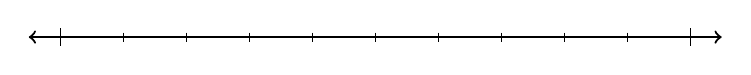
\begin{tikzpicture}[scale=0.8]
% a straight line segment
\draw [thick, <->] (-0.5,0) -- (10.5,0);
% the ticks and their labels
 \draw[xshift=0 cm] (0pt,4pt) -- (0pt,-4pt) ; 
\foreach \x  in {1,...,9}
  \draw[xshift=\x cm] (0pt,2pt) -- (0pt,-2pt);
 \draw[xshift=10 cm] (0pt,4pt) -- (0pt,-4pt) ; 
\end{tikzpicture}

\vspace{0.4cm}

\item How would your plotted points in the four number lines have been different if the number had been 341.7?  What about 0.003417?  Or 34,170,000?   What does your answer say about the consistent structure of the base-ten place value system?  (Hint:  In each number, how does the meaning of the 4 compare to the meaning of the 1 to its right?   How does the meaning of the 4 compare to the meaning of the 3 to its left?)  

\item How would your plotted points in the four number lines have been different if the number had been 3.41708?  What about 3.41708667999?  Explain.  

\item You should know or be able to figure out (in your head) decimal equivalents of fractions with many small  or ``nice'' denominators (i.e., 2, 3, 4, 5, 6, 8, 9, 10, 11, 12, 16, 20, 25, 30, 40, and 50).  Describe how to figure out quickly any that you might forget.  

\item Here is a nice relationship between twelfths and eighths:  $1/8\approx 0.12$ and $1/12\approx 0.08$.  Find other such pairs, and explain why the pairs ``work'' this way.   

\item Compare the decimal representations of $\frac{1}{7}$, $\frac{2}{7}$, $\frac{3}{7}$, $\frac{4}{7}$, $\frac{5}{7}$, and  $\frac{6}{7}$.
\begin{enumerate}  
\item Notice that the repeating digits always appear in the same order.  Explain why this is the case.
\item Suppose you are able to remember the decimal representation of $\frac{1}{7}$.  Explain how to use that to write quickly the decimal representation of any of the other sevenths.  
\end{enumerate}

\item 
Compare the decimal representations of $\frac{1}{13}$, $\frac{2}{13}$, \dots,  $\frac{12}{13}$.  
\begin{enumerate}  
\item Describe carefully how the order of the digits is somewhat like and also different from what you noticed for sevenths.  
\item Explain why the decimal representations of thirteenths work as you described.
\end{enumerate}

\item Without a calculator, predict whether the decimal representations of the following numbers will terminate or not.  For those that terminate, predict the number of decimal places.  
\begin{enumerate}
\item $\dfrac{13}{400}$
\item $\dfrac{11}{70}$
\item $\dfrac{21}{70}$
\item $\dfrac{27}{6250}$
\item $\dfrac{23}{2^7\cdot 5^2}$
\item $\dfrac{23}{2^7\cdot 5^2\cdot 11}$
\item $\dfrac{22}{2^7\cdot 5^2\cdot 11}$
\end{enumerate}

\item The clearest way to demonstrate that a number is rational is to show that it satisfies the definition.  (What is the definition of a rational number?)  Show that the following numbers are rational:  
\begin{enumerate}
\item $0.\overline{324}$
\item $15.\overline{324}$
\item $0.15\overline{324}$
\item $0.2\overline{5643}$
\end{enumerate}


\subsection*{Generalizations}
\item Use long division to explain why the decimal representation of a rational number must either terminate or repeat.

\item Suppose $\frac{m}{n}$ is a rational number in lowest terms.  If the number's decimal representation terminates, what can you conclude about $m$ and about $n$?  Explain.  

\item Suppose $\frac{m}{n}$ is a rational number in lowest terms.  If you know the number's decimal representation repeats, what can you conclude about the number of repeating digits?  Explain.  

\item You have seen three types of decimal representations for rational numbers between 0 and 1:  terminating, repeating, and delayed-repeating.  Suppose that $m$ and $n$ are counting numbers with no common factors and $m<n$.  Explain why the type of decimal representation of $\frac{m}{n}$ depends only on $n$ and not on $m$.  Hint:  Consider the three types separately.  

\subsection*{Explorations}

\item The rational number $\frac{1}{19}$ has decimal representation $0.\overline{052631578947368421}$.  To verify this, your calculator is unlikely to display enough digits, and long division would be quite tedious.  Devise a method for ``piecing together'' this decimal representation in ``chunks,'' using your calculator.  Then use the method to compute the decimal representation of $\frac{7}{23}$.  Be sure to indicate how you know that it repeats as you claim.  

\item Given a prime number $p$, find the smallest positive integer $n$ so that $p$ divides $10^n-1$, or explain why there is no such integer $n$.  
\begin{enumerate}
\item Do this for all primes less than 15, and also for the primes 37, 41, 73, and 101.
\item For each prime, compare the $n$ you found with the number of repeating digits in the decimal representation of $\frac{1}{p}$.  
Make a conjecture about what you notice.  Provide a brief explanation of why your conjecture ought to be true. 
\end{enumerate}

% In the following two problems, keep in mind that you are trying to explain arithmetic of decimals, which you will teach in grade 5.  
% So your explanations should NOT USE arithmetic of decimals.  Use fractions and the meanings of 
% decimals instead.  And it would be better if you do not use %negative exponents, which is in grade 8.

\item Explain $2.7\times 3.4$ in \textbf{two different ways}.  Be sure your explanations address two key questions:  (i) Why can you almost ignore the decimal point and multiply as though the digits described whole numbers?  And (ii) How do you know where to place the decimal point in the result?  Here are some ideas:  
\begin{itemize}
\item Use behind the scenes algebra to explain why the digits in the  $27\times 34$ should be the same as the digits in the desired product $2.7\times 3.4$.  
\item Convert the decimals to fractions, compute the product of the fractions, and then convert the result to a decimal.  
\item Use the picture below to compute $2.7\times 3.4$ with neither an algorithm nor a calculator.  Explain your reasoning.  
\[
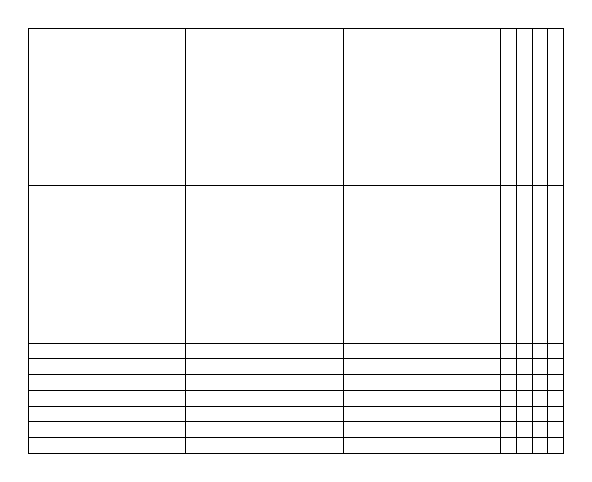
\begin{tikzpicture}[scale=2]
%\draw [line width=0.1pt,gray!30,step=1mm] (0,0) grid (3.4,2.7);
%\draw [help lines] (0,0) grid (3.4,2.7);
\draw (0,0) grid (3,2);
\draw [xstep=1cm,ystep=1mm] (0,-0.7) grid (3,0);
\draw [xstep=1mm,ystep=1cm] (3,0) grid (3.4,2);
\draw [xstep=1mm,ystep=1mm] (3,-0.7) grid (3.4,0);
\end{tikzpicture}
\]
\item Explain why the above picture can also represent $27\times 34$.  Explain the lengths and areas for both calculations.  

\end{itemize}

\item Explain $3.96\div 2.4$ in \textbf{two different ways}.  Be sure your explanations address two key questions:  (i) Why can you almost ignore the decimal point and divide as though the digits described whole numbers?  And (ii) How do you know where to place the decimal point in the result?  Here are some ideas:  
\begin{itemize}
\item Use the measurement model of division to reason how many groups of size $2.4$ are in $3.96$.
\item Use bundles or base ten blocks where the single stick or unit block represents a quantity other than 1.  
\item Multiply both the dividend and the divisor by a suitable power of 10 and then divide.  
\item Convert both decimals to fractions, divide the fractions, then convert the result back to a decimal.  
\item Divide $396$ by $24$ and then use estimation to place the decimal point.  
\end{itemize}

\end{enumerate}
\end{problems}





\chapter{Ratios, Functions, and Beyond}

\section{Ratios and Proportional Relationships}
As a topic in school mathematics, ratios and proportions are often isolated entities with their own special vocabulary, habits, and procedures.  When studying ratios and proportional situations, students often learn, ``Set up a proportion and cross multiply.''   But what is a proportion?  When does cross multiplication work?  Why does it work?  

For the problems in this section, try to take a more general approach:  ``Write an equation and solve.''  More precisely, ``Write an equation relating the quantities, and solve the equation for the desired quantity (usually an unknown).''  These are skills that serve students well throughout school mathematics and beyond.  

As you work through the problems and activities for this section, you will find it useful to make use of reasoning tools such as the following:  
\begin{itemize}
\item Equivalent fractions
\item Equivalent ratios
\item Ratio tables
\item Unit rates
\item Double number lines
\item Graphs
\end{itemize}

During the process, be on the lookout for a wide variety of strategies, including part:part comparisons, part:whole comparisons, common denominators, and common numerators.  And note how the problems simultaneously build on understandings of fractions and pave the way for functions.  

\subsection{Ratios}
Fractions, ratios, and rates are three connected ideas with differing histories and differing usage: 
\begin{itemize} 
\item \emph{Fractions} are numbers, often used to express results of sharing, cutting, or measuring.  
\item \emph{Ratios} have historically been used to compare quantities of the same kind, such as two lengths or two volumes.  Ratios are often expressed as pairs of counting numbers, without units, e.g., $3:2$.  
\item \emph{Rates} are typically used to compare different quantities (e.g., meters and seconds).  Rates are often expressed as quotients with units (e.g., 1.5 m/sec).  
\end{itemize} 

In high school and beyond, these rough historical distinctions become blurred, and the uses of these terms are varied, sometimes conflicting, and often muddled.  Thus, we will not attempt to write precise definitions that distinguish these terms from one another.  Instead, we aim toward the end-goal that students see all of these as quotients that provide differing perspectives on closely related ideas.  

To this end, we invest our energy in solving problems.  We will see that it is sometimes useful to attend only to the numbers in a situation, so that we can notice that two apparently different problems are abstractly the same if we ``decontextualize'' the problem by removing the units.  At other times, we will see the importance of using the units to interpret answers in context.  This interplay is the essence of modeling.

\fixnote{It would help to have some discussion of ``unit'' as 1, unit in measurement, and unit in a unit rate.}

\begin{teachingnote}
You will find insightful discussion and pictures in the draft 6-7 Progression on Ratios and Proportional Relationships, available at 

\url{http://math.arizona.edu/~ime/progressions/}
\end{teachingnote}

\subsection{Proportional Relationships}
For situations that involve two varying quantities, perhaps the most fundamental are those in which the quantities are proportional to one another.  
\begin{definition}
Quantities $x$ and $y$ are in a \emph{proportional relationship} if there is a constant $k$ such that $y=kx$.  
\end{definition}
When solving problems, a critical skill is the ability to distinguish propotional situations from situations in which quantities are not proportional.  
\begin{question}
Give a table of data for two quantities that are in a proportional relationship.  
\end{question}
\QM

\begin{question}
Give a table of data for two quantities that are \textbf{not} in a proportional relationship.  
\end{question}
\QM


\begin{activitynote}
Activities \ref{A:ratioLaunch}, \ref{A:ratios},  and \ref{A:ratioOddities} complement this section well. 
%% Ratio Launch
%% Poor Old Horatio
%% Ratio Oddities
%% Problem Solved
As a conclusion, we suggest doing Activity \ref{A:dreadedStoryProblem}.
\end{activitynote}

\newpage
\begin{problems}

\fixnote{Need easy problems, strip diagrams, double number lines.  See Beckmann.} 

\begin{enumerate}
\item A baseball coach once asked me the following question: If a
  pitcher can throw a 90 mph pitch during a game, but can only
  sustain a 60 mph pitch during practice, how close should the pitcher
  stand during practice to ensure that the amount of time it takes the
  ball to reach home plate is the same in practice as it is in the
  game? Explain your reasoning.

\item Three brothers and a sister won the lottery together and plan to
  share it equally. If the brothers alone had shared the money, then
  they would have increased the amount they each received by \$20. How
  much was won in the lottery? Explain your reasoning.

\item Chris is working on his Fiat. His car's cooling system holds 6
  quarts of coolant, and should be filled with a 50/50 mix of antifreeze 
and water. Chris noticed that the car was 1 quart low with the correct 50/50 mix.  
But then he added a 25/75 mix, 25 parts antifreeze, and 75 parts water.  How
  much coolant does he have to remove from the cooling system to then
  add 100 percent antifreeze to restore his desired 50/50 mix? Explain
  your reasoning.

\item If a hen and a half lays an egg and a half in a day and a half, 
how many eggs will 6 hens lay in 4 days?  How many days will it take for 
8 hens to lay 16 eggs?  How many hens would it take to lay 12 eggs in 
three days?  How many hens would it take to lay a dozen eggs per week?  
In each case, explain your reasoning.  

\item Fred and Frank are two fitness fanatics on a run from $A$ to
  $B$. Fred runs half the way and walks the other half. Frank runs for
  half the time and walks for the other half. They both run at the
  same speed and they both walk at the same speed. Who finishes first?
\begin{enumerate}
\item Before any computations are done, guess the
  solution to this problem and record your guess.  
\item Try to get a feel for this problem by choosing numbers for the
  unknowns and doing some calculations. What do these calculations say
  about your initial guess?
\item Use algebra to solve the problem.  What does your solution say 
about your initial guess?  
\end{enumerate}

\item Andy and Sandy run a race of a certain distance. When Sandy finishes, 
she is $1/10$ of the distance ahead of Andy, who then finishes the race. 
After some discussion, Andy and Sandy decide to race the distance again, but this time Sandy
  will start $1/10$ of the distance behind Andy (at the starting line) to ``even-up'' the
  competition. Who wins this time?  Explain your reasoning.  
\begin{enumerate}
\item Before any computations are done, guess the
  solution to this problem and record your guess.  
\item Try to get a feel for this problem by choosing numbers for the
  unknowns and doing some calculations. What do these calculations say
  about your initial guess?
\item Use algebra to solve the problem.  What does your solution say 
about your initial guess?  
\end{enumerate}

\item You have two beakers, one that contains water and another that
  contains an equal amount of oil. A certain amount of water is
  transferred to the oil and thoroughly mixed. Immediately, the same
  amount of the mixture is transferred back to the water. Is there now
  more water in the oil or is there more oil in the water?
\begin{enumerate}
\item Before any computations are done, guess the
  solution to this problem and record your guess.
\item Try to get a feel for this problem by choosing numbers for the
  unknowns and doing some calculations. What do these calculations say
  about your initial guess?
\item Use algebra to solve the problem.  What does your solution say 
about your initial guess?  
\end{enumerate}

\item While on a backpacking trip Lisa hiked five hours, first along a
  level path, then up a hill, then turned around and hiked back to her
  base camp along the same route. She walks $4$ miles per hour on a
  level trail, $3$ uphill, and $6$ downhill. Find the total distance
  traveled. Explain your reasoning.
\item Monica, Tessa, and Jim are grading papers. If it would take
  Monica $2$ hours to grade them all by herself, Tessa $3$ hours to
  grade them all by herself, and Jim $4$ hours to grade them all by
  himself how long would it take them to grade the exams if they all
  work together? Explain your reasoning.
\item Say quickly, friend, in what portion of a day will four
  fountains, being let loose together, fill a container which would
  be filled by the individual fountains in one day, half a day, a
  third of a day, and a sixth of a day respectively? Explain your
  reasoning---note this is an old problem from the Indian text
  \textit{Lilavati} written in the 1200s.
\item Three drops of \textit{Monica's XXX Hot Sauce} were mixed with
  five cups of chili mix to make a spicy treat---the hot sauce is much
  hotter than the chili. Later, two drops of \textit{Monica's XXX Hot
    Sauce} were mixed with three cups of chili. Which mixture is
  hotter? 

Josh made the following observation:  ``If two different recipes are added 
together, the result will be a chili with hotness between the two.''  Explain
why this makes sense.  

To compare the given recipes, Josh suggested using this reasoning backwards, 
as follows:  
 
\begin{itemize}
\item Remove the second (recipe) from the first, that is: Start with 3
  drops of hot sauce and 5 cups of chili, and remove 2 drops and 3
  cups. So we are now comparing
\[
\text{1 drop and 2 cups}\qquad\text{with}\qquad\text{2 drops and 3 cups.}
\]
\item Now remove the first from the second, that is: Start with 2
  drops and 3 cups, and remove 1 drop and 2 cups. So we are now
  comparing
\[
\text{1 drop and 2 cups}\qquad\text{with}\qquad\text{1 drop and 1
  cup.}
\]
\end{itemize}
Now you can see that the second is more concentrated (and hence
hotter!) than the first. Is this correct? Will this strategy
always/ever work? Explain your reasoning.
\end{enumerate}
\end{problems}

\section{Sequences and Functions}
\paragraph{Sequences.}  Because "Sequences and Series" is a common topic in calculus and precalculus courses, the concept of sequence is often considered an advanced topic in high schools, but the idea of a sequence is much more elementary.  In fact, many patterns explored in grades K-8 can be considered sequences.  For example, the sequence $4, 7, 10, 13, 16, \dots$ might be described as a ``plus 3 pattern'' because terms are computed by adding 3 to the previous term.  
\begin{activitynote}
Activities \ref{A:walk} through \ref{A:ExponentRules} are intended for this section.  
%%  Walk the Line  \ref{A:walk} 
%%  Constant Amount Change  \ref{A:ConstantAmount}
%%  Constant Percentage (Ratio) Change  \ref{A:ConstantRatio}
%%  Rules of Exponents  \ref{A:ExponentRules}
%%  Garden Variety \ref{A:gardenVariety}
\end{activitynote}
\begin{definition}
A \textbf{sequence}\index{sequence} is an ordered set of numbers or other objects.  The numbers or objects are called the \textbf{terms} of the sequence.  
\end{definition}

\paragraph{Functions.}  In the Common Core State Standards, students begin formal study of functions in grade 8.\standard{8.F.1}  
In high school, the approach to functions becomes more formal, through the use of function notation and with explicit attention to the concepts of domain and range.\standardhs{F-IF.1}   

\begin{definition}
A \textbf{function}\index{function} is a rule in which each input value determines a corresponding output value.  The \textbf{domain}\index{domain} of a function is the set of input values.  The \textbf{range}\index{range} of the function is the set of output values.
\end{definition}

\paragraph{Sequences Are Functions.} As students begin formal study of functions, it makes sense to use their patterning experience as a foundation for understanding functions.\standardhs{F-IF.3}  To show how the sequence above can be considered a function, we need an \textit{index}, which indicates which term of the sequence we are talking about, and which serves as an input value to the function.  After deciding that the 4 corresponds to an index value of 1, we can make a table showing 
the correspondence.\marginfigure{\footnotesize\sffamily
      \begin{tabular}{c||c|c|c|c|c|c}
        $n$ & 1 & 2 & 3 & 4 & 5 & \dots \\
\hline
        $f(n)$ & 4 & 7 & 10 & 13 & 16 & \dots
      \end{tabular}
\normalfont}

%%  \margincomment{We recommend using subscript notation only in advanced high school courses.} 

Although sequences are sometimes notated with subscripts, function notation can help students remember that sequences are functions.  For example, the sequence can be described recursively by the rule $f(1) = 4$, $f(n+1) = f(n) + 3$ for $n \geq 2$.  Notice that the recursive definition requires both a starting value and a rule for computing subsequent terms.   
The sequence can also be described with the closed (or explicit) formula  $f(n) = 3n + 1$, for integers $n \geq 1$.  Notice that the domain (i.e., integers $n\geq 1$) is included as part of the description.  When a function is given without an explicit domain, the assumption is that the domain is all values for which the expression is valid.  Thus, the function $g(x) = 3x + 1$ appears to be essentially the same as the function $f$ because the formula is the same and because $f(n) = g(n)$ for all positive integers.  To see that the functions are different, observe that $g(2.5) = 8.5$, but $f(2.5)$ is undefined.  

A common habit in school mathematics is creating a table of $(x,y)$ pairs, plotting those pairs (as dots), and then ``connecting the dots.''  The above discussion demonstrates that this habit is sometimes not appropriate: A graph\marginfigure{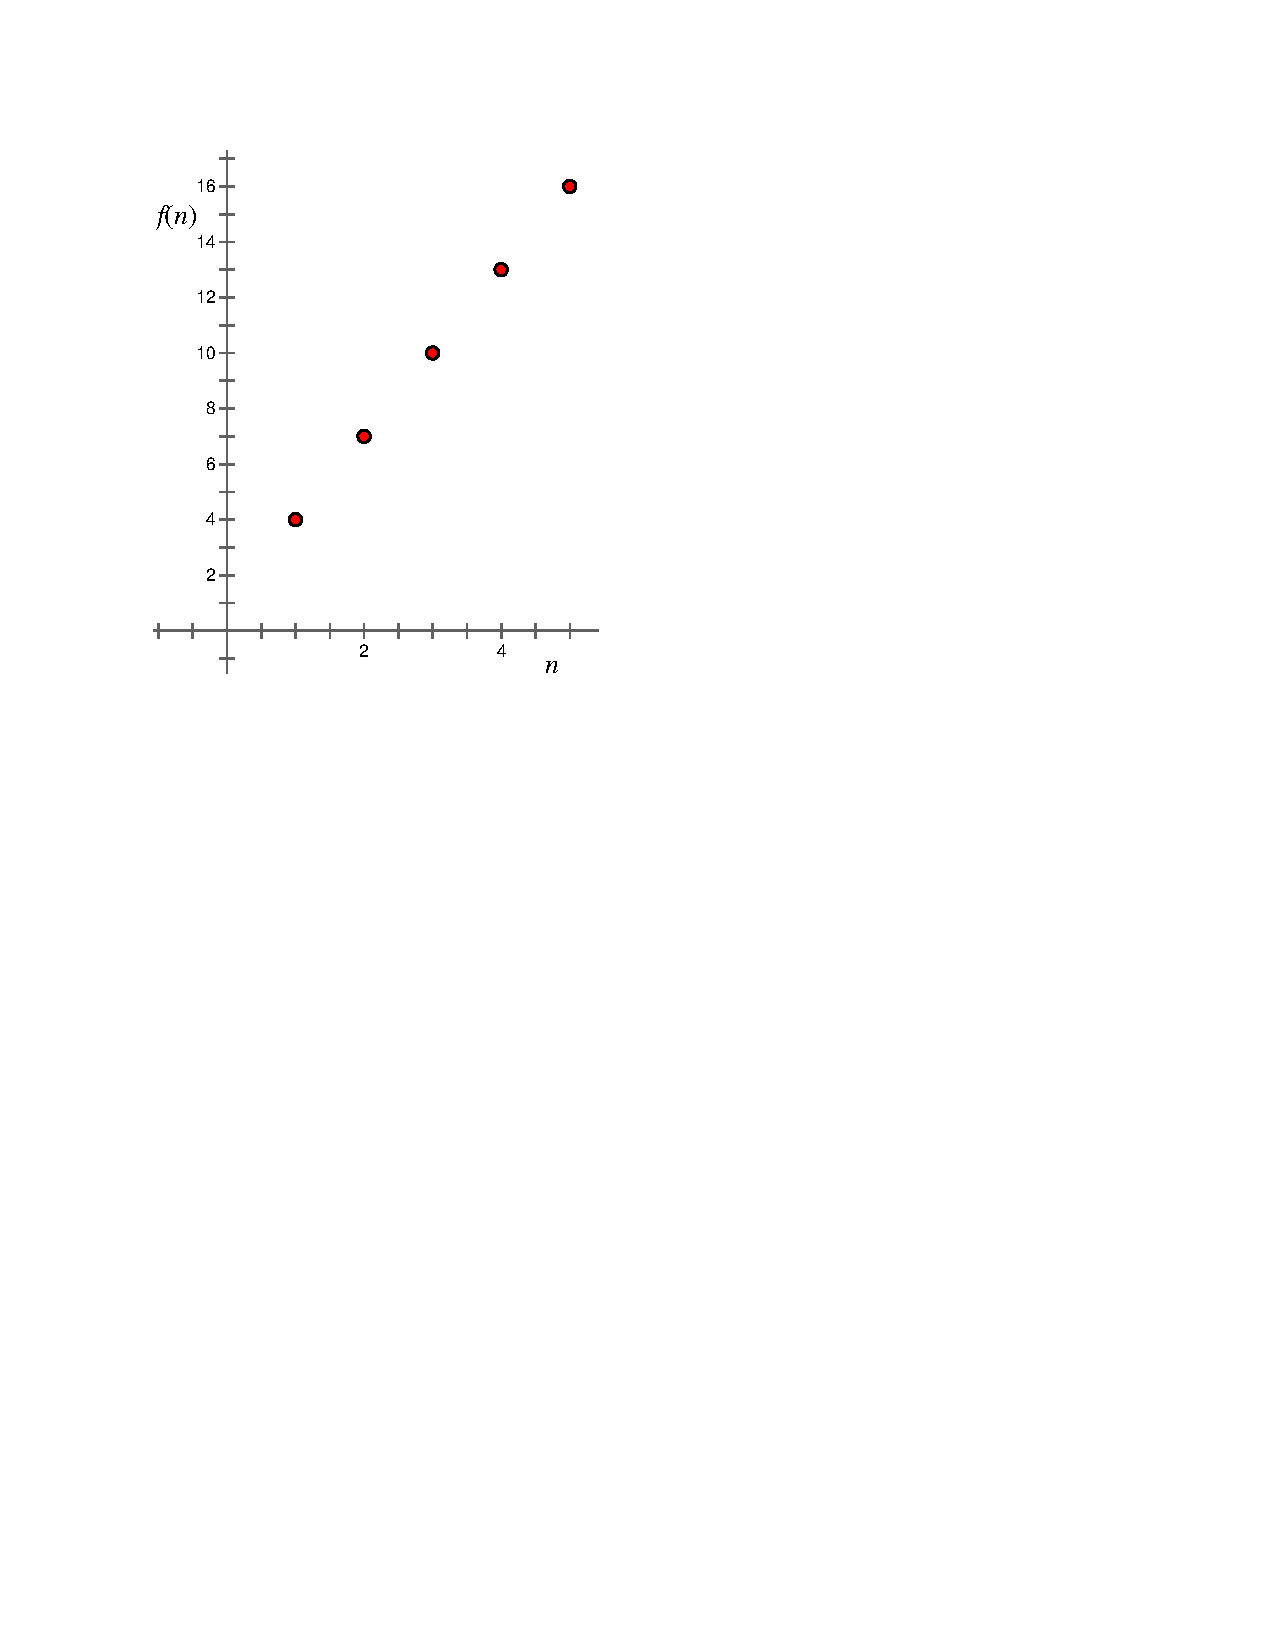
\includegraphics[width=2in]{../graphics/Graph-F2.pdf}} 
of the sequence consists of discrete dots, because the specification does not indicate what happens ``between the dots.''  Connecting the dots requires the assumption that domain values between the dots make sense in some way.  


\begin{question}
In your own words, what does it mean to say that sequences are functions?
\end{question}
\QM

\begin{question}
Given that $g(1) = 3$ and $g(n+1) = g(n) +4$ for integers $n>1$, find $g(6)$.  
Find a closed formula for $g(n)$.  
\end{question}
\QM

\begin{question}
Given that $f(1) = f(2) = 1$, and $f(n+1) = f(n)+f(n-1)$ for integers $n>2$, find $f(6)$.  
\end{question}
\QM

\paragraph{Arithmetic and Geometric Sequences.}Two types of sequences are especially important.\standardhs{F-BF.2}  
\begin{definition}
An \textbf{arithmetic sequence} any sequence that has a constant difference between consecutive terms.  A \textbf{geometric sequence} has a constant ratio between consecutive terms.  Some sequences, of course, are neither arithmetic nor geometric.
\end{definition}
\begin{question}
For each of the following sequences, decide whether it is arithmetic, geometric, or neither, and explain your reasoning:
\begin{itemize}  
\item $1, 4, 9, 16, 25, \dots$
\item $4, 8, 16, 32, \dots$
\item $2, 4, 6, 8, 2, 4, 6, 8, \dots$
\item $-2, 5, 12, 19, \dots$
\end{itemize}
Can you write both recursive and explicit formulas for each of these sequences?  
\end{question}
\QM

Beginning in about grade 8, much of school mathematics is devoted to the study of linear, quadratic, and exponential functions.\standardhs{F-LE.2}  Here we provide only definitions and key questions about these types of functions.  

\begin{itemize}
\item A linear function is of the form $f(x) = ax + b$, where $a$ and $b$ are real numbers and $a\ne 0$.  What do $a$ and $b$ tell you about the linear function?  
\item A quadratic function is of the form $f(x) = ax^2 + bx + c$, where $a$,  $b$, and $c$ are real numbers and $a\ne 0$.  What do $a$, $b$, and $c$ tell you about the function?   
\item An exponential function is of the form $f(x)=ab^x$, where $a$ and $b$ are real numbers, $a\ne 0$, and $b>0$.  What do $a$ and $b$ tell you about the function? 
\end{itemize}

\begin{question}
Why do these definitions require that $a \ne 0$?  
\end{question}
\QM

\begin{question}
Why does the definition of exponential function require that $b > 0$?  What happens if $b=0$?  What happens if $b<0$?
\end{question}
\QM

How can you identify these types of functions in tables, graphs, symbols, and contexts?\standardhs{F-IF.4} \standardhs{F-IF.7}  
For example, how can you recognize the slope in the graph of a linear function?  What about in a table, in a symbolic expression, or in a context?  

\begin{question}
An arithmetic sequence is what kind of function?  Explain. 
\end{question}
\QM

\begin{question}
A geometric sequence is what kind of function?  Explain.  
\end{question}
\QM

\begin{question}
Sometimes quadratic functions are written in the form $f(x) = a(x-h)^2+k$, where $a$, $h$, and $k$ are real numbers and $a\ne 0$.  What do $a$, $k$, and $h$ tell you about the function?  What are the advantages and disadvantages of this form of a quadratic, as compared to the alternative form given above?  
\end{question}
\QM

\paragraph{Concluding Remarks.}  When studying arithmetic and geometric sequences, it is tempting to encapsulate common results into compact formulas.  But formulas are easily confused with one another and otherwise misremembered.  Furthermore, general formulas often obscure the ideas.  

\begin{question}
Find the missing terms in the following arithmetic sequence:  
$$\rule[-2pt]{25pt}{.5pt}, \rule[-2pt]{25pt}{.5pt},  2,  \rule[-2pt]{25pt}{.5pt}, \rule[-2pt]{25pt}{.5pt}, 6, \dots$$
Explain your reasoning.  
\end{question}

\begin{question}
Find exact values (not decimal approximations) for the missing terms in the following geometric sequence:  
$$\rule[-2pt]{25pt}{.5pt}, \rule[-2pt]{25pt}{.5pt},  2,  \rule[-2pt]{25pt}{.5pt},  \rule[-2pt]{25pt}{.5pt}, \rule[-2pt]{25pt}{.5pt}, 6, \dots$$
Explain your reasoning.  And describe how this problem and the rules of exponents might be used to explain the connection between radicals and exponents.  
\end{question}

\begin{question}
What key ideas behind arithmetic and geometric sequences did you use in the previous two problems? 
\end{question}

\begin{center}
\textbf{With the ideas, you can reconstruct the formulas you need.  And without the ideas, formulas are empty.}  
\end{center}

\newpage
\begin{problems}
\begin{enumerate}

\item A park consists of a row of circular gardens.  ``Garden \#0'' has radius 3 feet, and each successive garden after that has a radius 2 feet greater than the previous garden.  
\begin{enumerate}
\item Using tables as a guide, write both explicit and recursive representations that will allow us to predict the area of the $n^\mathrm{th}$ garden.
\item Make a graph that shows the areas of the gardens in the park.  Which variable do you plot on the horizontal axis?  Explain.  
\item Does it make sense to connect the dots on your graph?  Explain your reasoning.  
\item Using your table, compute the area differences between the successive gardens.  What do you notice?  Why does this happen?
\end{enumerate}
\item An oil spill starts out as a circle with radius 3 feet and is expanding outward in all directions at a rate of 2 feet per minute. 
\begin{enumerate}
\item Use tables, graphs, and formulas to describe the area of the oil region $x$ minutes after the spill.  
\item How is this question fundamentally different than that of the gardens?  
\item Dumb Question:  At any one time, how many different areas are possible for the oil region?
\end{enumerate}


%\begin{prob}
%\textbf{Domain in context.}  Recall that the domain of a function is the set of input values that make sense in the problem.  Consider the following problem contexts:  
%\begin{itemize}
%\item The County Fair costs \$7 for admission and \$4 for each ride.  
%\item A taxi company charges \$11 for the first mile (or fraction thereof) and \$4 for each additional mile (or fraction thereof).  
%\item The Halloween parade, moving at a constant speed, was at mile marker 7 at noon, and at mile marker 11 at 1 pm.  
%\end{itemize}
%Blair used the letters $f$, $g$, and $h$ to describe functions for these three contexts, respectively, and noticed that 
%$f(3)=g(3)=h(3)$.  When she found a single formula that seemed to work for all three contexts, she thought that the three functions were equal.  But when she drew careful graphs of the functions, she was able to see that although the functions agree on many input values, they also disagree on many others.  
%
%Recreate Blair's work.  For each function, describe the meanings of the input and output values.  Indicate the domain of each function, and extend the domain, where reasonable, to include 0, fractions that are not counting numbers, and negative values.  Be sure that both the input and output values fit the context.  Draw a graph for each function, and describe how the graphs show the ways that the functions are both the same and different.  
%\end{prob}
%
%\begin{prob}
%The table below represents population growth for a hypothetical rabbit population.  
%
%\begin{center}
%\begin{tabular}{|l|c|c|c|c|c|}
%\hline
%Time (yrs) & 0 & 1 & 2 & 3 & 4 \\ \hline
%Population & 100 & 180 & 325 & 583 & 1,050\\  \hline
%\end{tabular}
%\end{center}
%
%\begin{enumerate}
%\item Assuming the growth pattern continues, write an equation for the rabbit population $p$ for any year $n$ after the rabbits are first counted.  Explain what the numbers in your equation represent. 
%\item Use your equation and this context to explain the meaning of an exponent of $-3$.  
%\item Based on common knowledge about rabbit populations, what can you say about the domain of your model?  In other words, what are the $n$-values for which the model is potentially reasonable?  
%\item In order to explore the accuracy of your exponential model for this rabbit population, write an equation for the rabbit population $p$ for any month $m$ after the rabbits are first counted.  Show how you know that your new equation describes the same population of rabbits.  
%\end{enumerate}
%Note:  This problem is based upon Problem 3.1 from \emph{Growing, Growing, Growing}, an eighth grade unit from CMP2, the second edition units of the Connected Mathematics Program. 
%\end{prob}
%
%
%\begin{prob}
%Suppose we want to fill in the blanks in the following geometric sequence: 
%\[ 
%\rule[-2pt]{35pt}{.5pt}, \rule[-2pt]{35pt}{.5pt}, \quad 2, \rule[-2pt]{35pt}{.5pt}, \rule[-2pt]{35pt}{.5pt}, \rule[-2pt]{35pt}{.5pt}, 
%\quad 6, \rule[-2pt]{35pt}{.5pt}, \dots
%\]
%\begin{enumerate}
%\item Why would it be incorrect to place 3, 4, and 5 in these blanks between 2 and 6? 
%\item Find exact values (not decimal approximations) for the missing values. Explain your reasoning. 
%\item Amanda used radicals to solve this problem, but Justin used exponents. Explain how both approaches can be correct. 
%\item Suppose $b$ is $n$ terms after $a$ in a geometric sequence. Find the $k^{th}$ term after $a$. Explain your reasoning. 
%\end{enumerate}
%\end{prob}
%
%%4. Geometric Sequences.  A sequence of numbers is called a geometric sequence if there is a constant ratio between consecutive terms.  For example, 2, 10, 50, 250, … is a geometric sequence with a starting term of 2 and a constant ratio of 5.  
%% 7.	Fill in the missing terms in the following geometric sequences: 
%% 
%% a.	5, ____, 15, ____, _____, …
%% b.	4, ____, ____, 20, ____, ____, …
%% c.	____, ____, ____, ____, ____, ____, ____, 4, ____, 8, ____, ____, …
%

  
%\begin{prob}
%Another way to reason about the meanings of zero and negative exponents is to use contexts involving exponential growth.  Suppose a virulent species of algae is overtaking the surface of a pond.  When scientists first noticed the problem, the algae covered 9 square meters of the pond surface.  One day later, the algae covered 18 square meters.  
%\begin{enumerate}
%\item Assuming the algae cover doubles every day, what will the algae coverage be on day 5?
%\item Write an expression that gives the algae coverage on any day. 
%\item On what day will the algae cover the whole pond, which measures about 10,000 square meters?  What does your answer say about your expression in part b?  
%\item  Use your expression and the context to interpret 0 and negative integer exponents.  
%\end{enumerate}
%\end{prob}
%
%\begin{prob}
%To make sense of an exponent of 1/2, Drew suggested that if the algae covered 9 square meters at noon on day 0 and 18 square meters at noon on day 1, then at 1/2 day, there would be 13.5 square meters of algae, which is 1.5 times as much.  Kelsey pointed out that if there is 1.5 times as much algae after 1/2  day, then there would be $1.5\cdot1.5 = 2.25$ times as much algae after a full day, which does not fit the context.  
%\begin{enumerate}
%\item Assuming that the algae has a constant growth factor, how much algae should there be at  1/2  day?  
%\item How does this help determine what an exponent of 1/2 should mean?  Explain.
%\item How much algae will there be after 1/3 of a day?  Express your answer using exponents, and approximate it as a decimal.
%\end{enumerate}
%\end{prob}


\end{enumerate}
\fixnote{Need more problems.  Doubling time?  Half life?  Use the ones from HW 8, in comments above.}



\end{problems}

\newpage

\section{Series}  
\begin{definition}
A \textbf{series} is a sum of consecutive terms from a sequence.  A series with terms that form an arithmetic sequence is called an \textbf{arithmetic series}.  
\end{definition}

\begin{activitynote}
Activities \ref{A:arithmeticSeries} and \ref{A:geometicSeries} are intended for this section.  
\end{activitynote}

\begin{question}
Find the sum:  $1 + 3 + 5 + \dots + 4999.$  (First explain how you know this is an arithmetic series.)
\end{question}
\QM

In mathematics teaching and learning, it is useful to distinguish problems from  excercises. \emph{Problems} require that you formulate a solution strategy, whereas \emph{exercises} are about using a procedure that you have been taught.\margincomment{Problem solving is an essential part of mathematics.}  Whether a question is a problem or an exercise depends upon the learner.  
\begin{question}
Is the previous question a problem or an exercise for you?  
\end{question}

When analyzing any series, it is often useful to consider the \emph{sequence of partial sums}.  For example, in response to the above question, the sequence of partial sums is as follows:  $$1, \qquad 1 + 3, \qquad 1+ 3+5, \qquad 1+3+5+7, \qquad \dots$$

Sometimes you can see a pattern in the sequence of partial sums.  Making a conjecture about a pattern is a type of inductive reasoning.  Once you notice a pattern, an important next step is showing, deductively, that the pattern \emph{must} continue.  

For arithmetic series, here are some approaches that can lead to general deductive arguments for the sum: 

\begin{itemize}
\item Consider pairing the first term with the last term, the second term with the second-to-last term, and so on.  What do you notice about the sum of each of these pairs?  And how many such pairs are in the whole series?  
\item Consider the average of each of the same pairs.  How might those averages help determine the sum of the whole series?  
\item Consider writing the series backward immediately below a forward version, line up the terms, and then add vertically.  
\end{itemize}

\begin{question}
Use one of these approaches to show that the sum is what it is.  Can you use a picture to illustrate your reasoning?    
\end{question}
\QM

\begin{question}
When you consider the sequence of partial sums of an arithmetic series, what kind of function(s) can you get?  Explain.  
\end{question} 
\QM

\begin{definition}
A series with terms that form a geometric sequence is called a \textbf{geometric series}.  
\end{definition}

\begin{question}
Find the sum:  $\frac{2}{3}+\frac{2}{9}+\dots+\frac{2}{3^{10}}$.  (First explain how you know the series is geometric.)
\end{question}
\QM

For the question above, it is not hard to see a pattern in the sequence of partial sums.  In fact, it is reasonable to believe that the pattern holds for any (finite) partial sum of the infinite geometric series $\frac{2}{3}+\frac{2}{9}+\dots$.  But to show that the pattern always holds, we need a general argument.  

For geometric series, the techniques for arithmetic series do not carry over.  Instead, observe that if you multiply the series by the common ratio, the resulting series has most of the same terms as the original series.  Thus, the difference between the two series (i.e., subtract the two) is a short expression that is not hard to work with.  

\begin{question}
Use these ideas to show that the sum is what it is.  Can you use a picture to illustrate this sum?    
\end{question}
\QM

\begin{question}
Convert $0.\overline{42}$ to a fraction.  What connections do you see with geometric series?  
\end{question}
\QM

\begin{question}
Explain briefly the key ideas behind finding the sum of an arithmetic series. Then do the same for geometric series.  
\end{question}
\QM


\newpage
\begin{problems}
\begin{enumerate}


\item Recall the story of Gertrude the Gumchewer, who has an addiction to Xtra Sugarloaded Gum.  Each day, she goes to her always stocked storage vault and grabs gum to chew.  At the beginning of her habit, she chewed three pieces and then, each day, she chews eight more pieces than she chewed the day before to satisfy her ever-increasing cravings. We want to find out how many pieces of gum did Gertrude chew over the course of the first 973 days of her habit?

\item Assume now that Gertrude, at the beginning of her habit, chewed $m$
pieces of gum and then, each day, she chews $n$ more pieces than she
chewed the day before to satisfy her ever-increasing cravings.  How many pieces will she chew over the course of the first $k$
  days of her habit? Explain your formula and how you know it will work for any $m$, $n$ and $k$.  

\item Find the sum:
\[
19 + 26 + 33 + \dots + 1720
\]
Give a story problem that is represented by this sum.

\item Now remember the story of Billy the bouncing ball.  He is dropped from a height of 13 feet and each bounce goes up 92\% of the bounce before it.  Assume that the first time Billy hits the ground is bounce \#1.  How far did Billy travel over the course of 38 bounces (up to when he hits the ground on his 38th bounce)?  

\item Assume now that Billy the Bouncing Ball is dropped from a height of
$h$ feet. After each bounce, Billy goes up a distance equal to $r$
times the distance of the previous bounce. (For example, $r=.92$ above.)
\begin{enumerate}
\item How high will Billy go after the $k$th bounce?
\item How much distance will Billy travel over the course of $k$
  bounces (not including the height he went up after the $k$th
  bounce)?
\item If $r<1$, what can you say about Billy's bounces? What if $r=1$?
  What if $r>1$?
\end{enumerate}

\item Joey starts out with \$456.  He plays one hand of poker each day with the same stakes of \$10.  Because he doesn't know anything about poker, he is on an extended losing streak.  Write explicit and recursive representations for the amount of money Joey has after $n$ days.  
      
\item Suppose Buzz Aldrin could fold a piece of paper in half as many times as he wanted---for rectangular paper of any size.  How many folds would Buzz need for the thickness of the paper to reach or exceed the distance from the earth to the moon?  How many folds would it take to reach or exceed halfway to the moon?

\item A ball is thrown up in the air from a 200 foot cliff with an initial velocity of 15 feet per second.  What is the height of the ball at any time $t$?  Write explicit and recursive representations of the relationship between the time after the ball is thrown and its height above the base of the cliff.

\item While waiting for Mark Pi to arrive to address the Mathematics Party, the members all shake hands with one another.  When Mark Pi walks in, he shakes hands with only the big-wigs of the Party.  A total of 6357 handshakes took place that day, and no one shook hands with the same person more than once.  How many members were there?  How many big-wigs were there?

\item If you deposit \$347 at the beginning of each year (starting on Jan. 1, 2014), into an account that compounds interest annually at a rate of 6.7\%, how much will be in the account on January 2, 2056?

\item You take out a \$100,000 loan on Jan. 1, 2014 to buy one Michigan ticket.  The loan shark charges 13\% annual interest.  You agree to pay back the loan through equal annual payments beginning on Jan. 1, 2015 and ending with the final payment on Jan. 1, 2028.  How much should each annual payment be? How much interest will you pay over the course of the payment plan?  If you hit the lottery on Dec. 31, 2020 and decide to pay off the rest of the loan the next day, how much will you owe?

\item 5 mg of a drug are administered to a patient at the start of a treatment regimen.  Each day at the same time, 3 more mg of the drug is administered.  Assuming that the drug still dissipates by 21\% each day, how much of the drug will be in the body immediately following the 3$4^\mathrm{th}$ 3 mg dose?

\item Find the fractional representation of the number $0.78\overline{4396}$.

\item A park consists of a row of circular gardens.  The ``Garden 0'' has radius 3 feet, and each successive garden after that has a radius 2 feet longer than the previous garden.  If there are 37 gardens, how much total area would the gardens comprise?

\item During their hour play time, the two oldest Brady kids (Greg and Marcia) went to the park to play with their walkie-talkies.  They used them for an hour.  The next day, the next-oldest kid came along.  Because there were only two walkie-talkies, they needed to share so that each possible pair got equal time.  The next day, the next-oldest also came along.  This continued until on the ninth day, all ten kids were there wanting to use the walkie-talkies.  How much time did Greg and Marcia spend with each other on the walkie-talkies over the course of the nine days?

\item Find the total number of gifts given in the song ``The 365 Days of Christmas''.

\end{enumerate}
\end{problems}



\chapter{Solving Equations}


\begin{quote}

%If $A$ is success in life, then $A = x + y + z$. Work is $x$; $y$ is
%play; and $z$ is keeping your mouth shut.
Politics is for the moment. An equation is for eternity.

\hfill---Albert Einstein
\end{quote}


\begin{teachingnote}
In this section, we are developing the idea that numbers are solutions
to equations. Negative integers arise out of simple linear equations,
as do rationals. However, these are not enough to solve all polynomial
equations, and hence we need a ``larger'' number system.
\end{teachingnote}


\section{Time to get Real}

Remember the definition of a \textit{root} of a polynomial:

\begin{definition} A \textbf{root}\index{root} of a polynomial 
\[
a_nx^n + a_{n-1}x^{n-1} + \dots + a_1 x + a_0
\]
is a number $\alpha$ where
\[
a_n\alpha^n + a_{n-1}\alpha^{n-1} + \dots + a_1 \alpha + a_0 = 0.
\]
\end{definition}


OK---let's go! We know what integers are right? We know what rational
numbers are right?

\begin{question}
Remind me, what is $\Z$? What is $\Q$? What is the relationship between
these two sets of numbers?
\end{question}
While I do want \textbf{you} to think about this, I also want to tell
you my answer: $\Q$ is the set of solutions to linear polynomial
equations with coefficients in $\Z$.

\begin{question}
What-with-the-who-in-the-where-now?
\end{question}
\QM

Are these all the numbers we need? Well, let's see. Consider the
innocent equation:
\[
x^2 -2 = 0
\]

\begin{question}
Could $x^2 -2$ have rational roots?
\end{question}

\begin{teachingnote}
Here we essentially run through the proof of the rational roots test.
\end{teachingnote}

Stand back---I'll handle this. Remember, a root of $x^2-2$ is a number
that solves the equation
\[
x^2-2 = 0.
\]
So suppose that there are integers $a$ and $b$ where $a/b$ is a root
of $x^2 -2$ where $a$ and $b$ have no common factors. Then
\[
\left(\frac{a}{b}\right)^2 -2 = 0.
\]
So
\[
a^2 - 2b^2 = 0 \qquad\text{thus}\qquad a^2 = 2b^2.
\]
But $a$ and $b$ have no common factors---so by the Unique
Factorization Theorem \index{Unique Factorization Theorem}for the
integers, $b^2 = 1$. If you find this step confusing, check
  out Problem \ref{P:helper} in Section \ref{S:EA}. This tells us that
$a^2 = 2$ and that $a$ is an integer---impossible! So $x^2-2$ cannot
have rational roots.

Hmmm but now consider the plot of $y= x^2-2$:
\[
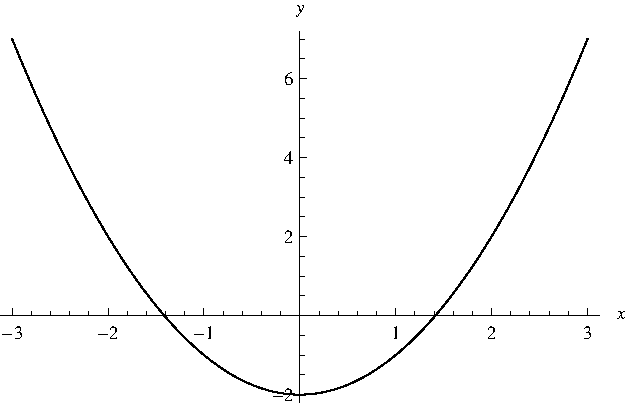
\includegraphics[width=3in]{../graphics/quad2Plot.pdf}
\]
The polynomial $x^2-2$ clearly has two roots! But we showed above that
neither of them are rational---this means that there must be numbers
that cannot be expressed as fractions of integers! In particular, this
means:\index{sqrt2@$\sqrt{2}$} 
\begin{center}
\textbf{The square-root of $\boldsymbol{2}$ is not rational!}
\end{center}
Wow! But it still can be written as a decimal
\[
\sqrt{2} = 1.4142135623\dots \index{sqrt2@$\sqrt{2}$}
\]
as the square-root of $2$ is a \textit{real number}.

\begin{definition}\index{R@$\R$}\index{real numbers} 
A \textbf{real number} is a number with a (possibly
infinite) decimal representation.  We use the symbol $\R$ to denote
the real numbers.
\end{definition}

For example:
\[
-1.000\dots \qquad 2.718281828459045\dots \qquad 3.333\dots \qquad 0.000\dots
\]
are all real numbers.

\begin{question} 
Another description of real numbers is that they are the numbers that
can be approximated by rational numbers. Why does this follow from the
definition above?
\end{question}
\QM

Famous examples of real numbers that are not rational are
\[\index{e@$e$}\index{pi@$\pi$}
\pi = 3.14159265358\dots\qquad \text{and}\qquad e = 2.718281828459045\dots
\]

\begin{question}
If $a$ and $b$ are integers with $b \ne 0$, what can you say about the
decimal representation of $a/b$? What can you say about the decimal
representation of an irrational number?
\end{question}
\QM




\begin{teachingnote}
Activities~\ref{A:DecNotNice} and~\ref{A:Shampoo} complement this section well. 
\end{teachingnote}




\newpage

\begin{problems}
\begin{enumerate}
\item Describe the set of real numbers. Give some relevant and
  revealing examples/nonexamples.
\item Explain what would happen if we ``declared'' the value of $\pi$
  to be $3$? What about if we declared it to have the value of $3.14$?
\item Explain why $x^2 - x - 1$ has no rational roots. 
\item Explain why $\sqrt{7}$ is irrational.
\item Explain why $\sqrt[3]{5}$ is irrational.
\item Explain why $\sqrt[5]{27}$ is irrational.
\item Explain why if $n$ is an integer and $\sqrt{n}$ is not an
  integer, then $n$ is irrational.
\item Consider the following numbers:
\[
\frac{1}{47} \qquad\text{and}\qquad \frac{1}{78125}
\]
For each, determine whether the decimal representation terminates or
repeates, \textbf{without} actually computing the decimal
representation. Explain your reasoning. If the decimal repeats,
indicate and explain what the maximum possible number of digits in the
repeating pattern is.
\item Solve $x^5 - 31x^4 +310x^3 -1240 x^2 + 1984x-1024= 0$. Interlace
  an explanation with your work. Hint: Use reasoning from this section
  to find rational roots.
\item Solve $x^5 - 28x^4 +288x^3 - 1358 x^2 + 2927 x -2310 =
  0$. Interlace an explanation with your work. Hint: Use reasoning
  from this section to find rational roots.
\item Knowing that $\pi$ is irrational, explain why $101\cdot\pi$ is
  irrational.
\item Knowing that $\pi$ is irrational, explain why $\pi + 101$ is
  irrational.
\item Knowing that $\pi$ is irrational, explain why $77.2835\cdot\pi$ is
  irrational.
\item Knowing that $\pi$ is irrational, explain why $\pi + 77.2835$ is
  irrational.
\item Suppose we knew that $\alpha^2$ was irrational. Could we
  conclude that $\alpha$ is also irrational? Explain your reasoning.
\item Is $((\sqrt{2})^{\sqrt{2}})^{\sqrt{2}}$ rational or irrational?
  Explain your reasoning.
\item In the discussion above, we give an argument showing that
  $\sqrt{2}$ is irrational. What happens if you try to use the exact
  same argument to try and show that $\sqrt{9}$ is irrational? Explain
  your reasoning.
\item For each of the following statements, indicate whether the expression
is a ``rational number,'' an ``irrational number,'' or whether it could be
either. Note, in parts (d)--(f) assume that neither numbers are zero.
\begin{enumerate}
\item $\text{rational}+ \text{rational} = ?$
\item $\text{rational}+ \text{irrational} = ?$
\item $\text{irrational}+ \text{irrational} = ?$

\item $\text{rational}\cdot \text{rational} = ?$
\item $\text{rational}\cdot \text{irrational} = ?$
\item $\text{irrational}\cdot \text{irrational} = ?$
\end{enumerate}
Give careful explanations for parts (a), (e), and (f).
\end{enumerate}
\end{problems}
\newpage




\section{Polynomial Equations}


\begin{teachingnote}
Activity~\ref{A:HAlgebra} is a good warm-up to this section. 
\end{teachingnote}

Solving equations is one of the fundamental activities in mathematics.
We're going to separate our equations into sets:
\begin{enumerate}
\item Linear Equations---polynomial equations of degree $1$.
\item Quadratic Equations---polynomial equations of degree $2$.
\item Cubic  Equations---polynomial equations of degree $3$.
\item Quartic Equations---polynomial equations of degree $4$.
\item Quintic Equations---polynomial equations of degree $5$.
\end{enumerate}
We'll stop right there, for now\dots


\subsection{Linear Equations}

The simplest polynomials (besides constant polynomials) are linear
polynomials. Solving equations of the form
\[
ax + b = 0
\]
poses no difficulty, we can write out the solution easily as
\[
x = -b/a.
\]


\begin{teachingnote}
Activity~\ref{A:walk} complements this section well. 
\end{teachingnote}


\subsection{Quadratic Equations}\index{completing the square}

Finding roots of quadratic polynomials is a bit more complex. We want
to find $x$ such that
\[
ax^2 + bx + c = 0.
\]
I know you already know how to do this. However, pretend for a moment
that you don't. This would be a really hard problem. We have evidence
that it took humans around 1000 years to solve this problem in
generality, the first general solution appearing in Babylon and China
around 2500 years ago. With this in mind, I think this topic warrants
some attention. If you want to solve $ax^2 + bx + c = 0$, a good place
to start would be with an easier problem. Let's make $a=1$ and try to
solve
\[
x^2 + b x = c
\]
Geometrically, you could visualize this as an $x \times x$ square
along with a $b\times x$ rectangle. Make a blob for $c$ on the other side. 

\begin{question} What would a picture of this look like?
\end{question}
\QM

\begin{question} What is the total area of the shapes in your picture?
\end{question}
\QM

Take your $b\times x$ rectangle and divide it into two
$(b/2)\times x$ rectangles.

\begin{question} What would a picture of this look like?
\end{question}
\QM

\begin{question} What is the total area of the shapes in your picture?
\end{question}
\QM

Now take both of your $(b/2)\times x$ rectangles and snuggie them
next to your $x\times x$ square on adjacent sides. You should now have
what looks like an $(x + \frac{b}{2}) \times (x +
\frac{b}{2})$ square with a corner cut out of it.


\begin{question} What would a picture of this look like?
\end{question}
\QM

\begin{question} What is the total area of the shapes in your picture?
\end{question}
\QM

Finally, your big $(x + \frac{b}{2}) \times (x + \frac{b}{2})$ has a
piece missing, a $(b/2) \times (b/2)$ square, right? So if you add
that piece in on both sides, the area of both sides of your picture
had better be $c + (b/2)^2$. From your picture you will find that:
\[
\left(x + \frac{b}{2}\right)^2 = c + \left(\frac{b}{2}\right)^2
\]

\begin{question} 
Can you find $x$ at this point?
\end{question}
\QM

\begin{question}
Explain how to solve $ax^2 + bx + c = 0$.
\end{question}
\QM




\begin{teachingnote}
Activities~\ref{A:otherSide},~\ref{A:vertex}, and~\ref{A:leastSquares},
complement this section well.
\end{teachingnote}

\begin{teachingnote}
Activity~\ref{A:otherCurves} could be done here too.
\end{teachingnote}

\subsection{Cubic Equations}

While the quadratic formula was discovered around 2500 years ago,
cubic equations proved to be a tougher nut to crack. A general
solution to a cubic equation was not found until the 1500's. At the
time mathematicians were a secretive and competitive bunch. Someone
would solve a particular cubic equation, then challenge another
mathematician to a sort of ``mathematical duel.'' Each mathematician
would give the other a list of problems to solve by a given date. The
one who solved the most problems was the winner and glory
everlasting\footnote{This might be a slight exaggeration.}  was
theirs. One of the greatest duelists was Niccol\`{o} Fontana Tartaglia
(pronounced \textit{Tar-tah-lee-ya}). Why was he so great? He
developed a general method for solving cubic equations! However,
neither was he alone in this discovery nor was he the first. As
sometimes happens, the method was discovered some years earlier by
another mathematician, Scipione del Ferro. However, due to the secrecy
and competitiveness, very few people knew of Ferro's method. Since these
discoveries were independent, we'll call the method the
\textit{Ferro-Tartaglia method}.

We'll show you the Ferro-Tartaglia method\index{Ferro-Tartaglia
  method} for finding at least one root of a cubic of the form:
\[
x^3+ px + q
\]
We'll illustrate with a specific example---you'll have to generalize
yourself! Take
\[
x^3 +3x - 2  = 0
\]
\paragraph{Step 1} Replace $x$ with $u+v$. 
\begin{align*}
(u+v)^3 + 3(u+v) - 2  &= u^3 + 3u^2v + 3uv^2 + v^3 + 3(u+v) -2 \\
&= u^3 + v^3 + 3uv(u+v) + 3(u+v) - 2\\
&= u^3 + v^3 - 2 + (3uv+3)(u+v).
\end{align*}
\paragraph{Step 2} 
Set $uv$ so that all of the terms are eliminated except for $u^3$,
$v^3$, and constant terms.  

Since we want 
\[
3uv + 3 = 0
\]
we'll set $uv = -1$ and so 
\[
u^3 + v^3 -2 = 0.
\]
Since $uv = -1$, we see that $v = -1/u$ so
\[
u^3 + \left(\frac{-1}{u}\right)^3  -2 = u^3 - \frac{1}{u^3} - 2= 0.
\]
\paragraph{Step 3} 
Clear denominators and use the quadratic formula.
\[
u^3 - \frac{1}{u^3} -2 = 0 \qquad \Leftrightarrow \qquad u^6 - 2 u^3 -1 = 0
\]
But now we may set $y = u^3$ and so we have
\[
y^2 - 2y -1 = 0
\]
and by the quadratic formula
\[
y = \frac{2 \pm \sqrt{4 + 4}}{2} = 1 \pm \sqrt{2}.
\]
Putting this all together we find:
\begin{align*}
y &= 1 \pm \sqrt{2} \\
u &= \sqrt[3]{1 \pm \sqrt{2}}\\
v &= \frac{-1}{\sqrt[3]{1 \pm \sqrt{2}}}
\end{align*}
and finally (drum-roll please):
\[
x = \sqrt[3]{1 + \sqrt{2}} - \frac{1}{\sqrt[3]{1 + \sqrt{2}}} \qquad\text{and}\qquad x = \sqrt[3]{1 - \sqrt{2}} - \frac{1}{\sqrt[3]{1 - \sqrt{2}}}
\]

\begin{question} How many solutions are we supposed to have in total?
\end{question}
\QM


\begin{question} How do we do this procedure for other equations of the form
\[
x^3 + px + q = 0?
\]
\end{question}
\QM



\subsection{Quartics, Quintics, and Beyond}

While the Ferro-Tartaglia method may seem like it only solves the
special case of $x^3 + px +q = 0$, it is in fact a ``wolf in sheep's
clothing''\index{wolf in sheep's clothing} and is the key to giving a
formula for solving any cubic equation
\[
ax^3 + bx^2 + cx +d = 0.
\]
The formula for solutions of the cubic equation is quite complex---we
will spare you the details. Despite the fact that the key step of the
formula is the Ferro-Tartaglia method, it is usually called
\textit{Cardano's formula}\index{Cardano's formula} because Cardano
was the first to publish this method.

It was wondered if there were formulas for solutions to polynomial
equations of arbitrary degree. When we say formulas, we mean formulas
involving the coefficients of the polynomials and the symbols:
\[
+\quad -\quad \cdot\quad \div \quad \sqrt{\hspace{1em}}
\]
Cardano's student Ferrari, (who incidentally went to the University of
Bologna) soon found the quartic formula, though it is too monstrous to
write down in these notes. The search for the quintic equation
began. Things started getting very difficult. The old tricks didn't
work, and it wasn't until nearly 300 years later that this problem was
settled.

\begin{question} 
Who was Niels Abel? Who was \'{E}variste
Galois?\index{Abel}\index{Galois}
\end{question}
\QM

Abel and Galois (pronounced \textit{Gal-wah}), independently prove
that there is no general formula (using only the symbols above) for
polynomial equations of degree $5$ or higher. It is an amazing result
and is only seen by students in advanced undergraduate or beginning
graduated courses in pure mathematics. Nevertheless, in our studies we
will not completely shy away from such demons. Read on!






\newpage

\begin{problems}
\begin{enumerate}
\item Draw a rough timeline showing: The point when we realized we
  were interested in quadratic equations, the discovery of the
  quadratic formula, the discovery of the cubic formula, the discovery
  of the quartic formula, and the work of Abel and Galois proving the
  impossibility of a general formula for polynomial equations of
  degree 5 or higher.
\item Given a polynomial, explain the connection between
  \textit{linear factors} and \textit{roots}. Are they the same thing
  or are they different things?
\item In ancient and Medieval times the discussion of quadratic
  equations was often broken into three cases:
\begin{enumerate}
\item $x^2 + bx = c$
\item $x^2 = bx + c$
\item $x^2 + c = bx$
\end{enumerate}
where $b$ and $c$ are positive numbers. Create real-world word
problems involving length and area for each case above.
\item In ancient and Medieval times the discussion of quadratic
  equations was often broken into three cases:
\begin{enumerate}
\item $x^2 + bx = c$
\item $x^2 = bx + c$
\item $x^2 + c = bx$
\end{enumerate}
where $b$ and $c$ are positive numbers.  Is this a complete list of
cases? If not, what is missing and why is it (are they)
missing? Explain your reasoning.
\item Describe what happens geometrically when you complete the square
  of a quadratic equation of the form $x^2 + bx = c$ when $b$ and $c$
  are positive. Explain your reasoning.
\item Jim, Lydia, and Isabel are visiting China. Unfortunately they are
  stuck in a seemingly infinite traffic jam. The cars are moving at a
  very slow (but constant) rate. Jim and Lydia are 25 miles behind
  Isabel. Jim wants to send a sandwich to Isabel. So he hops on his
  motorcycle and rides through traffic to Isabel, gives her the
  sandwich, and rides back to Lydia at a constant speed. When he
  returns to Lydia, she has moved all the way to where Isabel was when
  Jim started. In total, how far did Jim travel on his motorcycle?
\begin{enumerate}
\item Before any computations are done, use common sense to guess the
  solution to this problem.
\item Try to get a feel for this problem by choosing numbers for the
  unknowns and doing some calculations. What do these calculations say
  about your guess?
\item Use algebra to solve the problem.
\end{enumerate}
\item Must a quadratic polynomial always have a real root? Explain
  your reasoning.
\item Must a cubic polynomial always have a real root? Explain your
  reasoning.
\item Must a quartic polynomial always have a real root? Explain your
  reasoning.
\item Must a quintic polynomial always have a real root? Explain your
  reasoning.
\item Derive the quadratic formula. Explain your reasoning.
\item Solve $x^2 + 3x -2 = 0$. Interlace an explanation with your work.
\item Find two solutions to $x^4 + 3x^2 -2 = 0$. Interlace an
  explanation with your work.
\item Find two solutions to $x^6 + 3x^3 -2 = 0$. Interlace an
  explanation with your work.
\item Find two solutions to $x^{10} + 3x^5 -2 = 0$. Interlace an
  explanation with your work.
\item Find two solutions to $3x^{14} - 2x^7 + 6 = 0$. Interlace an
  explanation with your work.
\item Find two solutions to $-4x^{22} + 13x^{11} + 1 = 0$. Interlace
  an explanation with your work.
\item Give a general formula for finding two solutions to equations of
  the form: $ax^{2n} + bx^{n} + c = 0$ where $n$ is an
  integer. Interlace an explanation with your work.
\item Use the Ferro-Tartaglia method to find a solution to $x^3+x+1 =
  0$. Interlace an explanation with your work.
\item Use the Ferro-Tartaglia method to find a solution to $x^3-x-1 =
  0$. Interlace an explanation with your work.
\item Use the Ferro-Tartaglia method to find a solution to $x^3+3x-4 =
  0$. Interlace an explanation with your work.
\item Use the Ferro-Tartaglia method to find a solution to $x^3+2x-3 =
  0$. Interlace an explanation with your work.
\item Use the Ferro-Tartaglia method to find a solution to $x^3+6x-20 =
  0$. Interlace an explanation with your work.
\item Find at least two solutions to $x^4-x^3-3x^2+2x+1 =0$. Hint: Can
  you ``guess'' a solution to get you started?  Interlace an
  explanation with your work.
\item Explain what Abel and Galois proved to be impossible.
\end{enumerate}
\end{problems}





\section{Me, Myself, and a Complex Number}

\begin{teachingnote}
Activity~\ref{A:sketchRoots}, complements this section well.
\end{teachingnote}


We'll start with the definition:

\begin{definition} 
A \textbf{complex number}\index{C@$\C$}\index{complex!numbers} is a
number of the form
\[
x + yi
\]
where $x$ and $y$ are real numbers and $i$ is the square-root of
negative one. We use the symbol $\C$ to denote the complex numbers.
\end{definition}

What's that I hear? Yells of protest telling me that no such number
exists? Well if it makes you feel any better, people denied the
existence of such numbers for a long time. It wasn't until the
$1800$'s until people finally changed their minds. Let's talk about
some ideas that helped. Consider the plot of $y = x^3-6x+1$:
\[
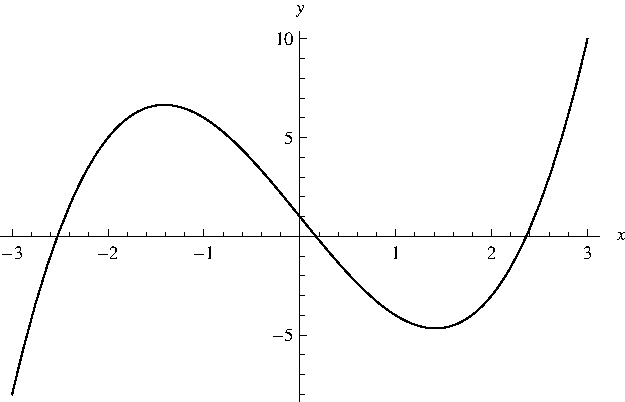
\includegraphics[width=3in]{../graphics/cubicPlot.pdf}
\]
If you use the Ferro-Tartaglia method to find at least one solution to
this cubic, then you find the following root:
\[
\sqrt[3]{\frac{-1+\sqrt{-31}}{2}} + \frac{2}{\sqrt[3]{\frac{1}{2}(-1+\sqrt{-31})}}
\]
This root looks like a complex number, since $\sqrt{-31}$ pops up
twice.  This might seem a bit redundant, but we should point out that
$\sqrt{-31}$ is a complex number since it can be expressed as:
\[
0 + \left(\sqrt{31}\right) i
\]
Even though our root has complex numbers in it, we know that it is
real from the picture!  Moral: If you want to give exact solutions to
equations, then you'd better work with complex numbers, even if the
roots are real!

\begin{teachingnote}
Here we are not ready to try to simplify the large expression
above. We are leaving this as a mystery for a future course.
\end{teachingnote}


\begin{question} If $u+vi$ is a nonzero complex number, is 
\[
\frac{1}{u+vi}
\]
a complex number too?
\end{question}

You betcha! Let's do it. The first thing you must do is multiply the
numerator and denominator by the complex conjugate of the denominator:
\[
\frac{1}{u+vi} = \frac{1}{u+vi} \cdot \frac{u-vi}{u-vi} =\frac{u-vi}{u^2 + v^2}
\]
Now break up your fraction into two fractions:
\[
\frac{u-vi}{u^2 + v^2} = \frac{u}{u^2 + v^2} + \frac{-v}{u^2+v^2}i
\]
Ah! Since $u$ and $v$ are real numbers, so are
\[
x = \frac{u}{u^2 + v^2} \qquad \text{and}\qquad y = \frac{-v}{u^2+v^2}
\]
Hence 
\[
\frac{1}{u+vi} = x + yi
\]
and is definitely a complex number.

The real importance of the complex numbers came from
Gauss,\index{Gauss} with the Fundamental Theorem of Algebra:

\begin{theorem}[Fundamental Theorem of Algebra]
\index{Fundamental Theorem!of Algebra} Every polynomial of the form
\[
 a_n x^n + a_{n-1} x^{n-1} + \dots + a_1 x + a_0
\]
where the $a_i$'s are complex numbers has exactly $n$ (possibly
repeated) complex roots.
\end{theorem}

Said a different way, the Fundamental Theorem of Algebra says that
every polynomial with complex coefficients
\[
a_n x^n + a_{n-1} x^{n-1} + \dots + a_1 x + a_0
\]
can be factored as 
\[
a_n\cdot (x-r_1)(x-r_2) \cdots (x-r_n)
\]
where each $r_i$ is a complex number.

\begin{question} 
How many complex roots does $x^3-1$ have? What are they?
\end{question}
\QM

\begin{teachingnote}
This problem should definitely be addressed. Again, we find an
obvious root, $x=1$ and use the division theorem.
\end{teachingnote}



\subsection{The Complex Plane}


\begin{teachingnote}
Activities~\ref{A:complexAddition} and~\ref{A:complexMultiplication}
complement this section well.
\end{teachingnote}

Complex numbers have a strong connection to geometry, we see this with
the \textit{complex plane}:

\begin{definition}
The \textbf{complex plane}\index{complex!plane} is obtained when one
plots the complex number $x + yi$ as the point $(x,y)$. When
considering the complex plane, the horizontal axis is called the
\textbf{real axis} and the vertical axis is called the
\textbf{imaginary axis}.
\end{definition}

Here is a grid. Draw the real and imaginary axes and plot the complex
numbers:
\[
3 \qquad -5i \qquad 4+6i \qquad -3+5i \qquad -6 -i \qquad 6-6i
\]
\[

\includegraphics{../graphics/complexPlane.pdf}
\]
Be sure to label your plot.


\begin{question} 
Geometrically speaking, what does it mean to ``add'' complex numbers?
\end{question}
\QM

\begin{question} 
Geometrically speaking, what does it mean to ``multiply'' complex numbers?
\end{question}
\QM

\begin{teachingnote}
The activities \ref{deg2Ext} and \ref{gaussianInt} are both rather
challenging, and can be skipped without real concern.
\end{teachingnote}


\newpage

\begin{problems}
\begin{enumerate}
\item What is a real number?
\item What is a complex number?
\item Solve $x^3-6x+5 = 0$ two different ways. First, try to find an
  ``obvious'' root, call it $r$. Then divide your polynomial by
  $(x-r)$ and find the remaining roots. Second, use the
  Ferro-Tartaglia method to find (at least) one solution. Compare your
  answers. What do you notice---explain your reasoning.
\item Solve $x^3-6x+4 = 0$ two different ways. First, try to find an
  ``obvious'' root, call it $r$. Then divide your polynomial by
  $(x-r)$ and find the remaining roots. Second, use the
  Ferro-Tartaglia method to find (at least) one solution. Compare your
  answers. What do you notice---explain your reasoning.
\item Solve $x^3-2x-1 = 0$ two different ways. First, try to find an
  ``obvious'' root, call it $r$. Then divide your polynomial by
  $(x-r)$ and find the remaining roots. Second, use the
  Ferro-Tartaglia method to find (at least) one solution. Compare your
  answers. What do you notice---explain your reasoning.  Interlace an
  explanation with your work.
\item Solve $x^3-12x-8 = 0$ two different ways. First, try to find an
  ``obvious'' root, call it $r$. Then divide your polynomial by
  $(x-r)$ and find the remaining roots. Second, use the
  Ferro-Tartaglia method to find (at least) one solution. Compare your
  answers. What do you notice---explain your reasoning.  Interlace an
  explanation with your work.
\item Solve $x^3-3x^2+5x-3 = 0$. Hint: Can you ``guess'' a solution to
  get you started?  Interlace an explanation with your work.
\item Solve $x^3+4x^2-7x+2 = 0$. Hint: Can you ``guess'' a solution to
  get you started?  Interlace an explanation with your work.
\item Draw a Venn diagram showing the relationship between $\Z$, $\Q$,
  $\R$, and $\C$. Include relevant examples of numbers belonging to
  each set.
\item Explain why the following ``joke'' is ``funny:'' \textit{The
  number you have dialed is imaginary. Please rotate your phone by 90
  degrees and try again.}
\item Explain why every real number is a complex number.
\item Explain why $\sqrt{-2}$ is a complex number. 
\item Is $\sqrt[3]{-2}$ a complex number? Explain your reasoning.
\item Explain why $\sqrt[10]{-5}$ is a complex number.
\item Explain why if $x+yi$ and $u+vi$ are complex numbers, then 
\[
(x+yi) +(u+vi)
\]
is a complex number.
\item Explain why if $x+yi$ and $u+vi$ are complex numbers, then 
\[
(x+yi)(u+vi)
\]
is a complex number.
\item Given a complex number $z = x + yi$, the \textbf{complex conjugate} of\index{complex!conjugate}
  $z$ is $x-yi$, we denote this as $\bar{z}$. Let $w = u+vi$ be
  another complex number.
\begin{enumerate}
\item Explain why $\bar{z}+\bar{w} = \bar{z+w}$.
\item Explain why $\bar{z}\cdot\bar{w} = \bar{z\cdot w}$.
\end{enumerate}
\item Explain why if $u+vi$ is a complex number, then
\[
\frac{1}{u+vi}
\]
is a complex number.
\item Compute the following, expressing your answer in the form
  $x + yi$:
\begin{enumerate}
\item $(1 + 2i)+ (1+7i)$
\item $(1 + 2i)\cdot (1+7i)$
\item $(1 + 2i)/(1+7i)$
\end{enumerate}
Explain your reasoning.
\item I'm going to show you something, see if you can see a connection to geometry:
\begin{enumerate}
\item Let $z = 3 + 4i$. Compute $\sqrt{z\cdot \bar{z}}$. 
\item Let $z = 6 + 8i$. Compute $\sqrt{z\cdot \bar{z}}$. 
\item Let $z = 5 + 12i$. Compute $\sqrt{z\cdot \bar{z}}$. 
\end{enumerate}
What do you notice?
\item\label{P:sqrti} Express $\sqrt{i}$ in the form $a + bi$. Hint: Solve the
  equation $z^2 = i$.
\item Factor the polynomial $3x^2 + 5x + 10$ over the complex
  numbers. Explain your reasoning.
\item Factor the polynomial $x^3-1$ over the complex numbers. Explain
  your reasoning.
\item Factor the polynomial $x^4-1$ over the complex numbers. Explain
  your reasoning.
\item Factor the polynomial $x^4+1$ over the complex numbers. Explain
  your reasoning. Hint: Factor as the difference of two squares and use Problem~\ref{P:sqrti}. 
\item Factor the polynomial $x^4+4$ over the complex numbers. Can it
  be factored into polynomials with real coefficients of lower degree?
  Explain your reasoning.
\item Plot all complex numbers $z$ in the complex plane such that
  $z\cdot \bar{z} =1$. Explain your reasoning.
\item\label{P:taylor} Suppose I told you that:
\begin{align*}
\sin(x) &= x - \frac{x^3}{3!} + \frac{x^5}{5!} - \frac{x^7}{7!} + \dots + \frac{(-1)^n x^{2n+1}}{(2n+1)!} + \cdots \\
\cos(x) &= 1 - \frac{x^2}{2!} + \frac{x^4}{4!} - \frac{x^6}{6!} + \dots + \frac{(-1)^n x^{2n}}{(2n)!} + \cdots \\
e^x &= 1 + x + \frac{x^2}{2!} + \frac{x^3}{3!} + \frac{x^4}{4!} + \dots + \frac{x^n}{n!} + \cdots 
\end{align*}
Explain why we say:
\[
e^{x\cdot i} = \cos(x) + i \sin(x)
\]
\item This is Euler's famous formula:
\[
e^{\pi \cdot i } + 1 = 0
\]
Use Problem \ref{P:taylor} to explain why it is true.
\item How many complex roots should $x^2 = 1$ have? What are they?
  Plot them in the complex plane.  Explain your reasoning.
\item How many complex roots should $x^3 = 1$ have? What are they?
  Plot them in the complex plane.  Explain your reasoning.
\item How many complex roots should $x^4 = 1$ have? What are they?
  Plot them in the complex plane.  Explain your reasoning.
\item How many complex roots should $x^5 = 1$ have? What are they?
  Plot them in the complex plane.  Explain your reasoning.




\end{enumerate}
\end{problems}
%%
%% Add cube root of unity, w
%% u+v
%% wu + v
%% u + wv
%%




\chapter{Harmony of Numbers}

\begin{quote}
%Nature uses as little as possible of anything.  

Let us despise the barbaric neighings [of war] which echo through
these noble lands, and awaken our understanding and longing for the
harmonies.

\hfill---Johannes Kepler
\end{quote}

\begin{teachingnote}
This section is a hodge-podge of applications and modeling.
\end{teachingnote}

\begin{activitynote}
Activity~\ref{A:orderMod} complements this section well.
\end{activitynote}

\section{Clocks}

It is now time to think about clocks. Consider the usual run-of-the-mill clock:
\[
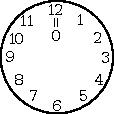
\includegraphics{../graphics/clock.pdf}
\]
\begin{question}
Suppose you start grading papers at $3$ o'clock and then $5$ hours
pass. What time is it? Now suppose that you find more papers to grade,
and $5$ more hours pass---now what time is it? How do you do these
problems? Why are there so many papers to grade?
\end{question}
\QM

We have a mathematical way of writing these questions:
\begin{align*}
3 + 5 &\equiv 8 \pmod{12} \\
8 + 5 &\equiv 1 \pmod{12} 
\end{align*}
We call arithmetic on clocks \textbf{modular arithmetic}.
\index{modular arithmetic} Being rather fearless in our quest for
knowledge, we aren't content to stick with $12$ hour clocks:
\[
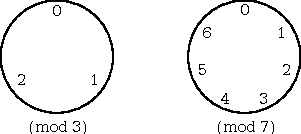
\includegraphics{../graphics/moreclocks.pdf}
\]

\begin{question}
Suppose you are working on a $2$ hour clock:
\[
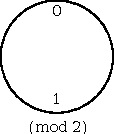
\includegraphics{../graphics/twoclock.pdf}
\]
Suppose you started at time zero, and finished after 10245
hours. 
\begin{enumerate}
\item Where is the hand of the clock pointing? 
\item How does the answer change if you are working on a $5$ hour
  clock?
\item What if you are working on a $7$ hour clock?
\end{enumerate}
\end{question}
\QM




OK---clocks are great. Here is something slightly different: Denote
the set of all integers that are $r$ greater than a multiple of $5$ by
$[r]_5$. So for example:
\[
[0]_5 = \{\dots,-15,-10,-5,0,5,10,15,\dots\}
\]
Write down the following sets:
\begin{align*}
[1]_5 &=  \raisebox{-3mm}{\fbox{\rule[0mm]{0mm}{7mm}\hspace{50ex}}} \\
[2]_5 &=  \raisebox{-3mm}{\fbox{\rule[0mm]{0mm}{7mm}\hspace{50ex}}} \\
[3]_5 &=  \raisebox{-3mm}{\fbox{\rule[0mm]{0mm}{7mm}\hspace{50ex}}} \\
[4]_5 &=  \raisebox{-3mm}{\fbox{\rule[0mm]{0mm}{7mm}\hspace{50ex}}} \\
[5]_5 &=  \raisebox{-3mm}{\fbox{\rule[0mm]{0mm}{7mm}\hspace{50ex}}} 
\end{align*}

\begin{question} With our work above, see if you can answer the following:
\begin{enumerate}
\item Explain why one could say that $[4]_5 = [9]_5$.
\item Explain why one could say that $[2]_5 = [-3]_5$.
\item Explain what you think is meant by the expression:
\[
[1]_5 + [2]_5 = [3]_5
\]
\item Explain what you think is meant by the expression:
\[
[1]_5 + [4]_5 = [0]_5
\]
\end{enumerate}
\end{question}
\QM



\begin{question}
How many different descriptions of modular arithmetic can you give? To aid you in this quest, I suggest you start your descriptions off with the words:
\begin{quote}
The number $a$ is congruent to $b$ modulo $m$ when \dots
\end{quote}
\end{question}
\QM

OK---I know I was supposed to leave that question for you, but there
is one description that I just gotta tell you about---check this out:
\[
a \equiv b \pmod{m} \qquad \Leftrightarrow \qquad a - b = m\cdot q
\]

\begin{question} 
What is the deal with the junk above? What is $q$? How does it help
you solve congruences like
\[
3x \equiv 1 \pmod{11}?
\]
\end{question}
\QM

\begin{question}
Is it the case that 
\[
5+x \equiv 2 + x \pmod{3}
\]
for all integers $x$? Why or why not? Use each of the descriptions
of modular arithmetic above to answer this question.
\end{question}
\QM







\newpage

\begin{problems}
\begin{enumerate}
\item Solve the following equations/congruences, expressing your
  answer as a number between $0$ and the relevant modulus:
\begin{enumerate}
\item $3 + x = 10$
\item $3 + x \equiv 10 \pmod{12}$
\item $3 + x \equiv 10 \pmod{7}$
\item $3 + x \equiv 10 \pmod{6}$
\item $3 + x \equiv 10 \pmod{5}$
\item $3 + x \equiv 10 \pmod{3}$
\item $3 + x \equiv 10 \pmod{2}$
\end{enumerate}
In each case explain your reasoning.
\item Solve the following equations/congruences, expressing your
  answer as a number between $0$ and the relevant modulus:
\begin{enumerate}
\item $10 + x = 1$
\item $10 + x \equiv 1 \pmod{12}$
\item $10 + x \equiv 1 \pmod{11}$
\item $10 + x \equiv 1 \pmod{9}$
\item $10 + x \equiv 1 \pmod{5}$
\item $10 + x \equiv 1 \pmod{3}$
\item $10 + x \equiv 1 \pmod{2}$
\end{enumerate}
In each case explain your reasoning.
\item Solve the following equations/congruences, expressing your
  answer as a number between $0$ and the relevant modulus:
\begin{enumerate}
\item $217 + x = 1022$
\item $217 + x \equiv 1022 \pmod{100}$
\item $217 + x \equiv 1022 \pmod{20}$
\item $217 + x \equiv 1022 \pmod{12}$
\item $217 + x \equiv 1022 \pmod{5}$
\item $217 + x \equiv 1022 \pmod{3}$
\item $217 + x \equiv 1022 \pmod{2}$
\end{enumerate}
In each case explain your reasoning.
\item Solve the following equations/congruences, expressing your
  answer as a number between $0$ and the relevant modulus:
\begin{enumerate}
\item $11+x \equiv 7 \pmod{2}$
\item $11+x \equiv 7 \pmod{3}$
\item $11+x \equiv 7 \pmod{5}$
\item $11+x \equiv 7 \pmod{8}$
\item $11+x \equiv 7 \pmod{10}$
\end{enumerate}
In each case explain your reasoning.

\item List out $6$ elements of $[3]_4$, including 3 positive and 3
  negative elements. Explain your reasoning.
\item List out $6$ elements of $[6]_7$, including 3 positive and 3
  negative elements. Explain your reasoning.
\item List out $6$ elements of $[7]_6$, including 3 positive and 3
  negative elements. Explain your reasoning.

\item One day you walk into a mathematics classroom and you see the
  following written on the board:
\begin{align*}
[4]_6 &=\{\dots, -14,-8,-2,4,10,16,22,\dots\}\\
\left[\frac{1}{2}\right] &=\left\{\dots, \frac{-3}{-6}, \frac{-2}{-4},
\frac{-1}{-2}, \frac{1}{2}, \frac{2}{4},\frac{3}{6},\dots\right\} 
\end{align*}
What is going on here? Can you figure out what $\left[\dfrac{3}{4}\right]$ would
be? Explain your reasoning.

\item If possible, solve the following equations/congruences,
  expressing your answer as a number between $0$ and the relevant
  modulus:
\begin{enumerate}
\item $3x = 1$
\item $3x \equiv 1 \pmod{11}$
\item $3x \equiv 1 \pmod{9}$
\item $3x \equiv 1 \pmod{8}$
\item $3x \equiv 1 \pmod{7}$
\item $3x \equiv 1 \pmod{3}$
\item $3x \equiv 1 \pmod{2}$
\end{enumerate}
In each case explain your reasoning.
\item Solve the following congruences, expressing your answer as a
  number between $0$ and the relevant modulus:
\begin{enumerate}
\item $11x \equiv 7 \pmod{2}$
\item $11x \equiv 7 \pmod{3}$
\item $11x \equiv 7 \pmod{5}$
\item $11x \equiv 7 \pmod{8}$
\item $11x \equiv 7 \pmod{10}$
\end{enumerate}
In each case explain your reasoning.
\item Solve the following congruences or explain why there is no
  solution, expressing your answer as a number between $0$ and the
  relevant modulus:
\begin{enumerate}
\item $15x \equiv 7 \pmod{2}$
\item $15x \equiv 7 \pmod{3}$
\item $15x \equiv 7 \pmod{5}$
\item $15x \equiv 7 \pmod{9}$
\item $15x \equiv 7 \pmod{10}$
\end{enumerate}
In each case explain your reasoning.
\item Make an ``addition table'' for arithmetic modulo $6$.
\item Make an ``addition table'' for arithmetic modulo $7$.
\item Make a ``multiplication table'' for arithmetic modulo $6$.
\item Make a ``multiplication table'' for arithmetic modulo $7$.

\item Explain the connection between writing an integer in base $b$ and
  reducing an integer modulo $b$.

\item Is 
\[
5 + x \equiv 12 + x \pmod{3}
\]
ever/always true? Explain your reasoning.
\item Is 
\[
20 + x \equiv 32 + x \pmod{3}
\]
ever/always true? Explain your reasoning.

\item Recalling that $i^2 = -1$, can you find ``$i$'' in the
  integers modulo $5$?  Explain your reasoning.
\item Recalling that $i^2 = -1$, can you find ``$i$'' in the
  integers modulo $17$?
  Explain your reasoning.
\item Recalling that $i^2 = -1$, can you find ``$i$'' in the
  integers modulo $13$?
  Explain your reasoning.
\item Recalling that $i^2 = -1$, can you find ``$i$'' in the
  integers modulo $11$?  Explain your reasoning.


\item Today is Saturday. What day will it be in 3281 days? Explain
  your reasoning.
\item It is now December. What month will it be in 219 months? What
  about 111 months ago? Explain your reasoning.
\item What is the remainder when $2^{999}$ is divided by $3$? Explain
  your reasoning.
\item What is the remainder when $3^{26}$ is divided by $7$? Explain
  your reasoning.
\item What is the remainder when $14^{30}$ is divided by $11$? Explain
  your reasoning.
\item What is the remainder when $5^{28}$ is divided by $11$? Explain
  your reasoning.
\item What is the units digit of $123^{456}$? Explain your reasoning.

\item Factor $x^2 + 1$ over the integers modulo $2$. Explain your
  reasoning.
\item Factor $x^3 +x^2 +x+1$ over the integers modulo $2$. Explain your
  reasoning.
\item Factor $x^5 +x^4 +x+1$ over the integers modulo $2$. Explain your
  reasoning.

\end{enumerate}
\end{problems}






\section{In the Real World}

Perhaps the coolest thing about mathematics is that you can actually
solve ``real world'' problems. Let's stroll through some of these
``real world'' problems.

\subsection{Automotive Repair}

\paragraph{A Geometry Problem}

One Thanksgiving Day I had a neat conversation with my cousin Chris at
the dinner table. You see he works on cars---specifically vintage
Italian sports cars. He had been doing some routine maintenance on one
of his cars and needed to remove the steering wheel and the steering
column.  All was fine until it came time to put the parts back
together. The steering wheel was no longer centered! The car could
drive down the street just fine, but when the car drove straight ahead
the steering wheel was off by a rotation of 5 degrees to the
right. This would not do!  This sounds like a geometry problem.


\paragraph{An Algebra Problem}

How did this happen you ask?  Well the
\index{steering!wheel}\textit{steering wheel} attaches to the car via
the \index{steering!column}\textit{steering column}:
\[
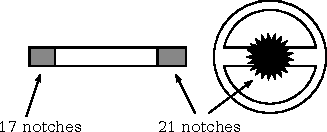
\includegraphics{../graphics/wheelcolumn.pdf}
\]
there were $21$ notches on the back of the wheel, which connects to
the column. There were also $17$ notches on the other end of the
column that then connected to the car itself.

Chris had noticed that moving the wheel 1 notch changed its position by 
\[
\frac{360}{21} \approx 17 \text{ degrees,}
\]
and that adjusting the columns by 1 notch changed its position by 
\[
\frac{360}{17} \approx 21 \text{ degrees.}
\]
Hmmm so if we want to center the wheel, we want to solve the following equation:
\[
17 w + 21 c = -5
\]
where $w$ represents how many notches we turn the wheel and $c$
represents how many notches we turn the column. Ah! This sounds like
an algebra problem! There is only one issue: We have two unknowns and
a single variable.


\begin{question}
How do we proceed from here? Can you solve the problem? Where does
modular arithmetic factor in to the solution?
\end{question}
\QM


\subsection{Check Digits}

Our world is full of numbers. Sometimes if you are in a large
organization---say a large university---you feel a bit like a
number. How do you know if you are the right number? Allow me to
clarify. Most items you buy have some sort of \index{UPC} UPC
(Universal Product Code) on them. This allows them to be put into a
computer in an organized fashion. When you buy items in a grocery
story, you want the item you scanned to come up---and not some other
(potentially embarrassing!) item. To ensure you get what is coming to
you, we have \index{check digits}\textit{check digits}. These are
digits that ``check'' to make sure that the code has scanned
correctly. Typically, what you see are either UPC-A codes or UPC-E
codes. Here is an example of a UPC-A code:
\[
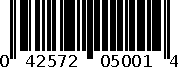
\includegraphics{../graphics/upcaEg.pdf}
\]
The check digit is the right most digit (in this case $4$). The check
digit is not used in identifying the item, instead it is used purely
to check if the other digits are correct. Here is how you check to see
if a UPC-A code is valid:
\begin{enumerate}
\item Working modulo $10$, add the digits in the odd positions and
  multiply by $3$:
\begin{align*}
0+2+7+0+0+1 &= 10\\
10\cdot 3 &= 30 \\
30 &\equiv 0 \pmod{10}.
\end{align*}
\item Working modulo $10$, add the digits in the even positions
  (including the check digit):
\begin{align*}
4+5+2+5+0 +4 &= 20 \\
20 &\equiv 0 \pmod{10}
\end{align*}
\item Add the outcomes from the previous steps together and take the
  result modulo $10$:
\[
0 + 0  \equiv 0 \pmod{10}
\]
\end{enumerate}
If the result is congruent to $0$ modulo $10$, as it is in this case,
then you have a correct UPC-A number and you are good to go!

We should note, sometimes at stores you see UPC-E codes:
\[

\includegraphics{../graphics/upceEg.pdf}
\]
%\begin{center}
%\begin{pspicture}(1.5,1.2in)
%\psbarcode{0123456}{includetext}{upce}
%\end{pspicture}
%\end{center}
These are compressed UPC-A codes where $5$ zeros have been
removed. The rules for transforming UPC-A codes to UPC-E codes are a
bit tedious, so we'll skip them for now---though they are easy
to look up on the internet.


\begin{question}
Can you find a UPC-E code and verify that it is valid?
\end{question}
\QM





\newpage

\begin{problems}
\begin{enumerate}

\item Which of the following is a correct UPC-A number?% telescope 
\begin{align*}
&8\quad12556\;01041\quad0\\
&8\quad12565\;01091\quad0\\
&8\quad12556\;01091\quad0
\end{align*}
Explain your reasoning.


\item  Which of the following is a correct UPC-A number?% telescope 
\begin{align*}
&7\quad17664\;13387\quad0\\
&7\quad17669\;13387\quad0\\
&7\quad17669\;73387\quad0
\end{align*}
Explain your reasoning.


\item Find the missing digit in the following UPC-A number:
\[
8\quad14371\;0\blacksquare354\quad2
\]
Explain your reasoning.

\item Find the missing digit in the following UPC-A number:
\[
0\quad76484\;86\blacksquare97\quad3
\]
Explain your reasoning.

\item How similar can two different UPC numbers be? Explain your
  reasoning.
\item In the United States some bank check codes are nine digit
  numbers
\[
a_1 a_2 a_3 a_4 a_5 a_6 a_7 a_8 a_9
\] 
where
\[
7a_1 + 3a_2 + 9a_3 + 7a_4 + 3a_5 + 9a_6 + 7 a_7 + 3a_8 \equiv a_9 \pmod{10}.
\]
\begin{enumerate}
\item Give three examples of valid bank check codes.
\item If adjacent digits were accidentally switched, could a machine
  detect the error? Explain your reasoning.
\end{enumerate}
\item ISBN-10 numbers are ten digit
  numbers
\[
a_1 a_2 a_3 a_4 a_5 a_6 a_7 a_8 a_9 a_{10}
\] 
where
\[
10a_1 + 9a_2 + 8a_3 + 7a_4 + 6a_5 + 5a_6 + 4a_7 + 3a_8 +2a_9+a_{10}\equiv 0 \pmod{11}.
\]
\begin{enumerate}
\item Give three examples of ISBN-10 numbers.
\item If adjacent digits were accidentally switched, could a machine
  detect the error? Explain your reasoning.
\end{enumerate}
\end{enumerate}
\end{problems}

\newpage



\section{The Binomial Theorem}


\subsection{Varna-Sangita}

In ancient Indian texts we find a description of a type of music
called \textit{varna-sangita}.\index{varna-sangita} This is music made
from a variation of long and short syllables. When performing a
varna-sangita, one starts off with a given number of short syllables
and ends with the same number of long syllables. In between these
verses, every possible combination of long and short syllables is
supposed to occur. If $s$ represents a short syllable and $l$
represents a long syllable we might visualize this as:
\[
ssss  \xto{\text{every possible combination}} llll
\]

To check their work, the people of ancient India counted how many of
each combination appeared in a song. Suppose we started with $sss$ and
finished with $lll$. Our song should contain the following verses:
\[
sss,\qquad ssl,\qquad sls, \qquad lss, \qquad sll,\qquad lsl, \qquad lls,\qquad lll
\]
We can construct the following table to summarize what we have found:
\[
\begin{tabular}{|c|c|c|c|}\hline
$3$ $s$'s & $2$ $s$'s and $1$ $l$ & $1$ $s$ and $2$ $l$'s & $3$ $l$'s \\ \hline
1 & 3 & 3 & 1\\\hline
\end{tabular}
\]

\begin{question} 
What would your table look like if you started with $ss$ and finished
with $ll$? What about if you started with $ssss$ and finished with
$llll$?
\end{question}
\QM

The vedics of the time gave a rule for making tables like the one
above. Their rule was based on the following diagram:
\[
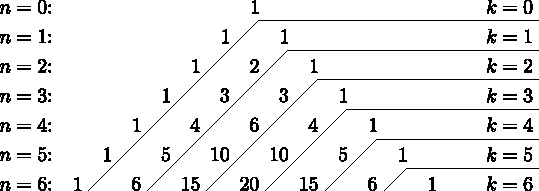
\includegraphics[scale=1]{../graphics/pascalsTri.pdf}
\]
Today people call this diagram \textbf{Pascal's
  triangle}.\index{Pascal's!triangle}
%\large %% Code used to help inkscape
%\[
%\begin{tabular}{rc@{}c@{}c@{}c@{}c@{}c@{}c@{}c@{}c@{}c@{}c@{}c@{}c@{}}
%$n=0$:&    &    &   &    &    &    &  1\\
%$n=1$:&    &    &   &    &    &  1 &    &  1\\
%$n=2$:&    &    &   &    &  1 &    &  2 &    &  1\\
%$n=3$:&    &    &   &  1 &    &  3 &    &  3 &    &  1\\
%$n=4$:&    &    & 1 &    &  4 &    &  6 &    &  4 &    &  1\\
%$n=5$:&    &  1 &    &  5 &    &  10 &    &  10 &    &  5 & & 1\\
%$n=6$:&  1 &    &  6 &    &  15 &    &  20 &    &  15 & & 6 & & 1\\
%\end{tabular}
%\]
%\[
%\begin{tabular}{r}
%$k=0$\\
%$k=1$\\
%$k=2$\\
%$k=3$\\
%$k=4$\\
%$k=5$\\
%$k=6$\\
%\end{tabular}
%\]

\begin{question}
How does Pascal's triangle relate to varna-sangitas? Is there an easy
way to produce the above diagram?
\end{question}
\QM

And now for something completely different\dots 

\subsection{Expansions}

Expand the following on a separate sheet of paper. Write the result
of your work in the boxes below:
\begin{align*}
(a + b)^0 &=  \raisebox{-3mm}{\fbox{\rule[0mm]{0mm}{7mm}\hspace{50ex}}} \\
(a + b)^1 &=  \raisebox{-3mm}{\fbox{\rule[0mm]{0mm}{7mm}\hspace{50ex}}} \\
(a + b)^2 &=  \raisebox{-3mm}{\fbox{\rule[0mm]{0mm}{7mm}\hspace{50ex}}} \\
(a + b)^3 &=  \raisebox{-3mm}{\fbox{\rule[0mm]{0mm}{7mm}\hspace{50ex}}} \\
(a + b)^4 &=  \raisebox{-3mm}{\fbox{\rule[0mm]{0mm}{7mm}\hspace{50ex}}} 
\end{align*}

\begin{question} Is there a nice way to organize this data?
\end{question}
\QM

\begin{question}
Can you explain the connection between expanding binomials and
varna-sangitas?
\end{question}
\QM

\begin{activitynote}
Activity~\ref{A:traffic} complements this section well.  % On the Road
\end{activitynote}



\subsection{Come Together}

Let's see if we can bring these ideas together. Let's denote the following symbol:
\[
\binom{n}{k} = \text{the number of ways we choose $k$ objects from $n$
  objects}.\index{nchoosek@$\binom{n}{k}$}\index{nck@$_nC_k$}
\]
it is often said ``$n$ choose $k$'' and is sometimes denoted as $_n C_k$.

\begin{question}
What exactly does $\binom{n}{k}$ mean in terms of varna-sangitas? What
does $\binom{n}{k}$ mean in terms of expansion of binomials?
\end{question}
\QM

\begin{question} How does $\binom{n}{k}$ relate to Pascal's triangle?
\end{question}
\QM


\begin{question}
Pascal claims:
\[
\binom{n}{k-1} +  \binom{n}{k} = \binom{n+1}{k}
\]
Explain how this single equation basically encapsulates the key
to constructing Pascal's triangle.
\end{question}
\QM

\begin{question}
Suppose that an oracle tells you that
\[
\binom{n}{k} = \frac{n!}{k!(n-k)!}
\]
but we, being good skeptical people, are not convinced. How do we
check this?
\end{question}
\QM

From the work above, we obtain a fabulous theorem:


\begin{theorem}[Binomial Theorem]\index{Binomial Theorem} 
If $n$ is a nonnegative integer, then
\[
(a+b)^n = \binom{n}{0} a^nb^0 + \binom{n}{1} a^{n-1}b^1 + \dots + \binom{n}{n-1} a^{1}b^{n-1} + \binom{n}{n} a^{0}b^n.   
\]
\end{theorem}


\begin{question} 
This looks like gibberish to me. Tell me what it is saying. Also, why
is the Binomial Theorem true?
\end{question}
\QM



\begin{activitynote}
Activity \ref{A:factOrFiction} complements this section well.  % Pascal's Triangle: Fact or Fiction
\end{activitynote}


\begin{activitynote}
Activity~\ref{A:pyramid} is worth considering here.  % Pascal's Pyramid
\end{activitynote}


\begin{activitynote}
The counting/probability activities, \ref{A:countOnIt} through \ref{A:fallForAnything} can now be done.
% You Can Count on It
% Which Road Should We Take
% Lumpy and Eddie
% Go Climb a Tree
% They'll Fall for Anything
\end{activitynote}



\newpage
\begin{problems}
\begin{enumerate}
\item Write down the first $7$ rows of Pascal's triangle.
\item Explain how $\binom{n}{k}$ corresponds to the entries of Pascal's
  triangle. Feel free to draw diagrams and give examples.
\item State the Binomial Theorem and give some examples of it in action.
\item Explain the ``physical'' meaning of $\binom{n}{k}$. Give some
  examples illustrating this meaning.
\item\label{P:bfor} Explain how Pascal's triangle is formed. In your
  explanation, use the notation $\binom{n}{k}$. If you were so
  inclined to do so, could you state a single equation that basically
  encapsulates your explanation above?
\item Explain why the formula you found in Problem \ref{P:bfor} is
  true.
\item State the formula for $\binom{n}{k}$.
\item Expand $(a + b)^5$ using the Binomial Theorem.
\item Expand $(a - b)^7$ using the Binomial Theorem.
\item Expand $(-a - b)^8$ using the Binomial Theorem.
\item Expand $(a + (b + c))^3$ using the Binomial Theorem.
\item Expand $(a - b - c)^3$ using the Binomial Theorem.
\item\label{P:exp1} Let $n$ be a positive integer.
\begin{enumerate}
\item Try some experiments to guess when $9^n + 1^n$ is
  divisible by $10$. What do you find? Clearly articulate your
  conjecture.
\item Use the Binomial Theorem to explain why your conjecture is
  true. Hint: $10-9 = 1$.
\end{enumerate}
\item\label{P:exp2} Let $n$ be a positive integer.
\begin{enumerate}
\item Try some experiments to guess when $6^n + 4^n$ is divisible by
  $10$. What do you find? Clearly articulate your conjecture.
\item Use the Binomial Theorem to explain why your conjecture is
  true. Hint: $10-6 = 4$.
\end{enumerate}
\item\label{P:exp3} Let $n$ be a positive integer.
\begin{enumerate}
\item Try some experiments to guess when $7^n - 3^n$ is divisible by
  $10$. What do you find? Clearly articulate your conjecture.
\item Use the Binomial Theorem to explain why your conjecture is
  true. Hint: $10-3 = 7$.
\end{enumerate}
\item\label{P:exp4} Let $n$ be a positive integer.
\begin{enumerate}
\item Try some experiments to guess when $8^n - 2^n$ is divisible by
  $10$. What do you find? Clearly articulate your conjecture.
\item Use the Binomial Theorem to explain why your conjecture is
  true. Hint: $10-2 = 8$.
\end{enumerate}
\item Generalize Problems \ref{P:exp1}, \ref{P:exp2}, \ref{P:exp3},
  and \ref{P:exp4} above. Clearly articulate your new statement(s) and
  explain why they are true.
\item\label{P:e1} Which is larger, $(1 + 1/2)^2$ or $2$? Explain your
  reasoning.
\item\label{P:e2} Which is larger, $(1 + 1/5)^5$ or $2$? Explain your
  reasoning.
\item\label{P:e3} Which is larger, $(1 + 1/27)^{27}$ or $2$? Explain
  your reasoning.
\item\label{P:e4} Which is larger, $(1 + 1/101)^{101}$ or $2$? Explain
  your reasoning.
\item\label{P:e5} Which is larger, $(1.0001)^{10000}$ or $2$? Explain
  your reasoning.
\item Generalize Problems \ref{P:e1}, \ref{P:e2}, \ref{P:e3},
  \ref{P:e4}, and \ref{P:e5} above. Clearly articulate your new
  statement(s) and explain why it is true.
\item Given a positive integer $n$, can you guess an upper bound for
  $(1 + 1/n)^{n}$?
\item Let $n$ be a positive integer. Use the Binomial Theorem to
  explain why:
\[
\binom{n}{0} + \binom{n}{1} + \binom{n}{2} + \dots + \binom{n}{n} = 2^n
\]
What does this mean in terms of Pascal's Triangle?
\item Let $n$ be a positive integer. Use the Binomial Theorem to
  explain why:
\[
(-1)^0\binom{n}{0} + (-1)^1\binom{n}{1} + (-1)^2\binom{n}{2} + \dots + (-1)^n\binom{n}{n} = 0
\]
What does this mean in terms of Pascal's Triangle?
\item Suppose I tell you:
\[
(1+x)^n = \binom{n}{0} + \binom{n}{1}x + \binom{n}{2}x^2+\dots +
\binom{n}{n}x^n
\]
Explain how to deduce:
\[
(a+b)^n = \binom{n}{0}a^n + \binom{n}{1}a^{n-1}b +
\binom{n}{2}a^{n-2}b^2+\dots + \binom{n}{n}b^n
\]
\end{enumerate}
\end{problems}






\appendix

\renewcommand{\theenumi}{$(\mathrm{\alph{enumi}})$}
\renewcommand{\labelenumi}{\theenumi}
\chapter{Activities}
%\addtocontents{toc}{\protect\setcounter{tocdepth}{0}}


%\newpage
\section{Shemp: A Prequel to Home Base}\label{A:shemp}

\begin{prob}
Long before recorded history, Shemp, a shepherd, wanted to make sure all his sheep returned from the field.  But back then, no one had any concept of ``counting.''  One day, Shemp found a big pile of necklaces big enough for sheep.  Shemp figured out a scheme, using a bunch of pegs hammered into his cave wall, that would help him know whether his sheep had come in from the field.  What do you think his scheme was?
\end{prob}

\begin{prob}
Eons later, two Stooges (shepherds who were using Shemp's necklace scheme) wanted to know who had ``more'' sheep.  They still had no concept of ``counting,'' but Moe figured out how to solve the problem by using the necklaces.  What do you think Moe did?
\end{prob}

\begin{prob}
Centuries later, the Stooges discovered that they could make marks on their cave walls instead of using pegs and necklaces.  So, for example, Grog might have this written on his cave wall:  $||||||||||||||||||||||||$ while Greg would have this on his cave wall:  $||||||||||||||||||$.  To see if their sheep had all returned, they would just point to one mark, then go on to the next, and the next, and so on (saying ``ni'' for each mark).  Now, when arguing over which had more, each could bring a papyrus copy of the cave wall markings.  How might this system work?
\end{prob}

\begin{prob}
Finally, Larry the Finer, invaded Stooge Valley and wanted to know ``how many'' sheep each shepherd had.  Since the Stooge People had never thought of the idea of ``how many,'' Larry told them to give different names to each of the marks on their wall.  How might this work?  
\end{prob}

\begin{prob}
But Larry was impatient.  If a shepherd's wall looked like $$|||||||||||||||||||||||||||||||||||||||||||||||||||||||||||||||||||||||||||||||||||||||||||||||||||||||||||||||||||||||||||||||||||||||||||||||||||$$
he couldn't tell quickly how many sheep there were.   Describe two or three steps that would solve Larry's problem.   
\end{prob}

\begin{prob}
What does it mean for someone to be able to ``count''?
\end{prob}
 

\newpage
\section{Shelby and Scotty}\label{A:SS}

Shelby and Scotty want to express the number $27$ in base
$4$. However, they used very different methods to do this. Let's check
them out.

\fixnote{Make the division symbols look better.}

\fixnote{Extensions in Vic's e-mail.  Bigger numbers, include a 0 in a digit.}

\fixnote{Perhaps swap the order.}

\fixnote{Convert 8630 (base ten) to base thirteen.  Quickly convert 2102 (base three) to base nine.}

\fixnote{Without using base ten, convert 341 (base six) to base four.  Without using base ten, convert 341 (base six) to base eleven.}


\begin{prob} Consider Shelby's work:
\[
4\,\begin{tabular}[b]{@{}r@{} r}
$6$ &\, R\,$\boldsymbol{3}$\\ \cline{1-1}
\Big)\begin{tabular}[t]{@{}l@{}}
$27$ 
\end{tabular}
\end{tabular}
\qquad
4\,\begin{tabular}[b]{@{}r@{} r}
$1$ &\, R\,$\boldsymbol{2}$\\ \cline{1-1}
\Big)\begin{tabular}[t]{@{}l@{}}
$6$ 
\end{tabular}
\end{tabular}
\qquad
4\,\begin{tabular}[b]{@{}r@{} r}
$0$ &\, R\,$\boldsymbol{1}$\\ \cline{1-1}
\Big)\begin{tabular}[t]{@{}l@{}}
$1$ 
\end{tabular}
\end{tabular} \qquad \Rightarrow \qquad \fbox{$123$}
\]
\begin{enumerate}
\item Describe how to perform this algorithm.
\item Provide an additional relevant and revealing example
  demonstrating that you understand the algorithm.
\end{enumerate}
\end{prob}




\begin{prob} Consider Scotty's work:
\[
4^3\,\begin{tabular}[b]{@{}r@{} r}
$0$ &\, R\,$27$\\ \cline{1-1}
\Big)\begin{tabular}[t]{@{}l@{}}
$27$ 
\end{tabular}
\end{tabular}
\qquad
4^2\,\begin{tabular}[b]{@{}r@{} r}
$\boldsymbol{1}$ &\, R\,$11$\\ \cline{1-1}
\Big)\begin{tabular}[t]{@{}l@{}}
$27$ 
\end{tabular}
\end{tabular}
\qquad
4\,\begin{tabular}[b]{@{}r@{} r}
$\boldsymbol{2}$ &\, R\,$\boldsymbol{3}$\\ \cline{1-1}
\Big)\begin{tabular}[t]{@{}l@{}}
$11$ 
\end{tabular}
\end{tabular} \qquad \Rightarrow \qquad \fbox{$123$}
\]
\begin{enumerate}
\item Describe how to perform this algorithm.
\item Provide an additional relevant and revealing example
  demonstrating that you understand the algorithm.
\end{enumerate}
\end{prob}

\begin{prob} 
Create an illustration (or series of illustrations) based on the $27$
marks below that models Shelby's method for changing bases.
\[
|\;\;|\;\;|\;\;|\;\;|\;\;|\;\;|\;\;|\;\;|\;\;|\;\;|\;\;|\;\;|\;\;|\;\;|\;\;|\;\;|\;\;|\;\;|\;\;|\;\;|\;\;|\;\;|\;\;|\;\;|\;\;|\;\;|
\]
Further, explain why Shelby's method works. 
\end{prob}

\begin{prob} 
Create an illustration (or series of illustrations) based on the $27$
marks below that models Scotty's method for changing bases.
\[
|\;\;|\;\;|\;\;|\;\;|\;\;|\;\;|\;\;|\;\;|\;\;|\;\;|\;\;|\;\;|\;\;|\;\;|\;\;|\;\;|\;\;|\;\;|\;\;|\;\;|\;\;|\;\;|\;\;|\;\;|\;\;|\;\;|
\]
Further, explain why Scotty's method works. 
\end{prob}
  % Shelby and Scotty

\newpage
\section{Hieroglyphical Arithmetic}\label{A:HAr}
\emph{Note: This activity is based on an activity originally designed by Lee Wayand.}

\fixnote{Perhaps include something about closure.}

%\symbolfootnote[0]{This activity is based on an activity originally designed by Lee Wayand.}

%\newcommand{\lo}{\vcenter{\hbox{\PHbee}}}
%\newcommand{\loo}{\vcenter{\hbox{\PHboomerang}}}
%\newcommand{\la}{\vcenter{\hbox{\PHcat}}}
%\newcommand{\lb}{\vcenter{\hbox{\PHdove}}}
%\newcommand{\lc}{\vcenter{\hbox{\PHpedestrian}}}
%\newcommand{\ld}{\vcenter{\hbox{\PHplaneTree}}}
%\newcommand{\lf}{\vcenter{\hbox{\PHplumedHead}}}
%\newcommand{\lh}{\vcenter{\hbox{\PHram}}}
%\newcommand{\li}{\vcenter{\hbox{\PHrosette}}}
%\newcommand{\lx}{\vcenter{\hbox{\PHsaw}}}
%\newcommand{\ly}{\vcenter{\hbox{\PHship}}}
%\newcommand{\lz}{\vcenter{\hbox{\PHstrainer}}}
%\newcommand{\lw}{\vcenter{\hbox{\PHtunny}}}

\newcommand{\lo}{\vcenter{\hbox{\textproto{a}}}}
\newcommand{\loo}{\vcenter{\hbox{\textproto{d}}}}
\newcommand{\la}{\vcenter{\hbox{\textproto{w}}}}
\newcommand{\lb}{\vcenter{\hbox{\textproto{H}}}}
\newcommand{\lc}{\vcenter{\hbox{\textproto{T}}}}
\newcommand{\ld}{\vcenter{\hbox{\textproto{K}}}}
\newcommand{\lf}{\vcenter{\hbox{\textproto{E}}}}
\newcommand{\lh}{\vcenter{\hbox{\textproto{l}}}}
\newcommand{\li}{\vcenter{\hbox{\textproto{o}}}}
\newcommand{\lx}{\vcenter{\hbox{\textproto{x}}}}
\newcommand{\ly}{\vcenter{\hbox{\textproto{R}}}}
\newcommand{\lz}{\vcenter{\hbox{\textproto{v}}}}
\newcommand{\lw}{\vcenter{\hbox{\textproto{q}}}}


Consider the following addition and multiplication tables:
\begin{fullwidth}
\[
{\renewcommand{\arraystretch}{1.8}
\begin{array}{clc}
{\renewcommand{\arraystretch}{1.8}
\begin{array}{|c||c|c|c|c|c|c|c|c|c|}\hline
 +  &\loo & \la & \lo & \lb & \lc & \ld & \lf & \lh & \li \\ \hline\hline
\loo& \ld & \lh &\loo & \li & \lb & \lo & \la & \lf & \lc \\ \hline
\la & \lh & \li & \la & \ld &\loo & \lf & \lb & \lc & \lo \\ \hline
\lo &\loo & \la & \lo & \lb & \lc & \ld & \lf & \lh & \li \\ \hline
\lb & \li & \ld & \lb & \lh & \la & \lc &\loo & \lo & \lf \\ \hline
\lc & \lb &\loo & \lc & \la & \lf & \li & \lo & \ld & \lh \\ \hline
\ld & \lo & \lf & \ld & \lc & \li &\loo & \lh & \la & \lb \\ \hline
\lf & \la & \lb & \lf &\loo & \lo & \lh & \lc & \li & \ld \\ \hline
\lh & \lf & \lc & \lh & \lo & \ld & \la & \li & \lb &\loo \\ \hline
\li & \lc & \lo & \li & \lf & \lh & \lb & \ld &\loo & \la \\ \hline
\end{array}}
\vspace{.5cm}
& 
\begin{array}{l}
\text{$\loo =$ fish} \\ 
\text{$\la =$ lolly-pop} \\ 
\text{$\lo =$ skull} \\ 
\text{$\lb =$ cinder-block} \\ 
\text{$\lc =$ DNA} \\ 
\text{$\ld =$ fork} \\ 
\text{$\lf =$ man} \\ 
\text{$\lh =$ balloon} \\ 
\text{$\li =$ eyeball} 
\end{array}
&
{\renewcommand{\arraystretch}{1.8}
\begin{array}{|c||c|c|c|c|c|c|c|c|c|}\hline
\cdot & \ld & \li & \lh & \lf & \lo & \la & \lb & \lc &\loo \\ \hline\hline
\ld   &\loo & \la & \lb & \lc & \lo & \li & \lh & \lf & \ld \\ \hline
\li   & \la & \lh & \lf & \ld & \lo & \lb & \lc &\loo & \li \\ \hline
\lh   & \lb & \lf & \ld & \la & \lo & \lc &\loo & \li & \lh \\ \hline
\lf   & \lc & \ld & \la & \lb & \lo &\loo & \li & \lh & \lf \\ \hline
\lo   & \lo & \lo & \lo & \lo & \lo & \lo & \lo & \lo & \lo \\ \hline
\la   & \li & \lb & \lc &\loo & \lo & \lh & \lf & \ld & \la \\ \hline
\lb   & \lh & \lc &\loo & \li & \lo & \lf & \ld & \la & \lb \\ \hline
\lc   & \lf &\loo & \li & \lh & \lo & \ld & \la & \lb & \lc \\ \hline
\loo  & \ld & \li & \lh & \lf & \lo & \la & \lb & \lc &\loo \\ \hline
\end{array}}
\end{array}}
\]
\end{fullwidth}
\newpage

\begin{prob} 
Use the addition table to compute the following:
\[
\lb + \la \qquad\text{and}\qquad \lc + \lf
\]
\end{prob}

\begin{prob} 
Do you notice any patterns in the addition table? Tell us about them.
\end{prob}

\begin{prob} 
Can you tell me which glyph represents $0$? How did you arrive at this
conclusion?
\end{prob}

\begin{prob} 
Use the multiplication table to compute the following:
\[
\li \cdot \lb \qquad\text{and}\qquad \la \cdot \lf
\]
\end{prob}

\begin{prob} 
Do you notice any patterns in the multiplication table? Tell us about them.
\end{prob}

\begin{prob} 
Can you tell me which glyph represents $1$? How did you arrive at this
conclusion?
\end{prob}


\begin{prob} Compute:
\[
\loo - \la \qquad\text{and}\qquad \ld - \lc
\]
\end{prob}



\begin{prob} Compute:
\[
\lf \div \lc \qquad\text{and}\qquad \lh \div \li
\]
\end{prob}

\begin{prob} 
Keen Kelley was working with our tables above. All of a sudden, she
writes
\[
\loo + \loo + \loo = \lo
\]
and shouts ``Weird!'' Why is she so surprised? Try repeated addition
with other glyphs. What do you find? Can you explain this?
\end{prob}


\begin{prob}
Can you find any other oddities of the arithmetic above? Hint: Try
repeated multiplication!
\end{prob}




\newpage
\section{Playing with Blocks}\label{A:B1}
\index{base-ten blocks} 

I always enjoyed blocks quite a bit. Go find yourself
some \textit{base-ten blocks}. Just so that we are all on the same
page, here are the basic blocks:
\[
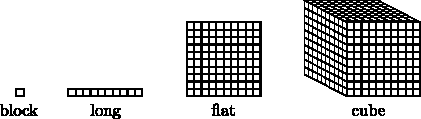
\includegraphics{../graphics/baseTenBlocks.pdf}
\]

\begin{prob} 
Sketch a model of the number $247$ with base-ten blocks.
\vspace{0.8in}
\end{prob}

\begin{prob}
Oscar modeled the number $15$ in the following way:
\[
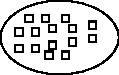
\includegraphics{../graphics/oscarModel.pdf}
\]
What do you think of his model?  Can you improve upon it?  
\vspace{0.5in}
\end{prob}

\begin{teachingnote}
The issue here is that the place-value system is not modeled. When
working with base-ten blocks, we will demand that the place value
system is always modeled.  We want to do this with all algorithms.  
\end{teachingnote}

\begin{prob}
Many problems involving subtraction can be considered one of the following types:  take-away, comparison, and missing addend.  Write a ``word problem'' illustrating each of these types.  
\end{prob}

\newpage

\begin{prob} 
Here is a standard subtraction algorithm:\index{subtraction algorithm!standard}
\[
\begin{tabular}{@{}r@{}r@{}r@{}r@{}}
&   & 8 &  \\
& 8 & $\not{\hspace{-.2ex}9}$ & $\hspace{.3ex}\leftexp{1}2$\\
$-$ & 3 & 7 & 8\\ \hline
& 5 & 1 & 4
\end{tabular}
\]
Use base-ten blocks to model this algorithm.  Which type of subtraction are you using?  
\end{prob}

\newpage
\fixnote{Maybe do the next problem before the previous.}
\begin{prob}
Oscar uses base-ten blocks to model subtraction.  
\[
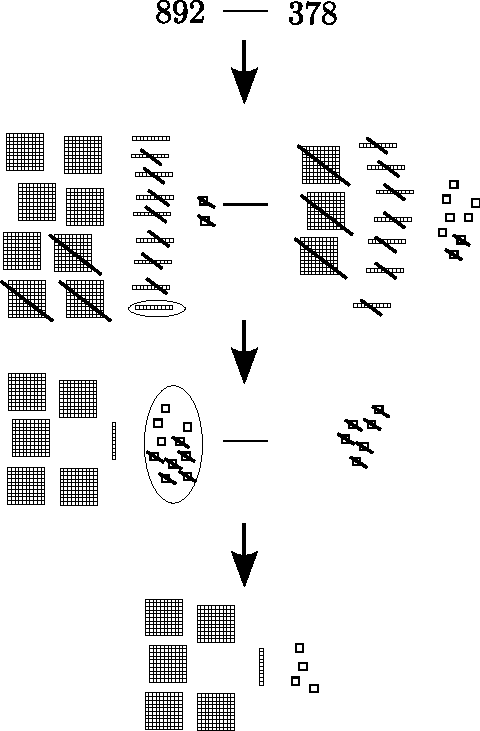
\includegraphics{../graphics/oscarSub.pdf}
\]
Can you explain what is going on?  Which type of subtraction is Oscar using?  
\end{prob}

\begin{prob} Create a ``new'' subtraction algorithm based on Oscar's model.
\end{prob}

\newpage
\begin{prob}
Here is an example of a standard addition algorithm:
\[
\begin{tabular}{@{}r@{}}
11~~\\
892\\
+398\\ \hline
1290
\end{tabular}
\]
Model this algorithm with base-ten blocks.
\end{prob}






\newpage
\section{More Playing with Blocks}\label{A:B2}
\index{base-ten blocks} 

Did you put your blocks away? Darn---there is still more to be
done! Just so that we are all on the same page, here are the basic
blocks:
\[
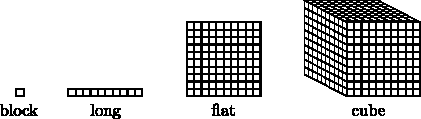
\includegraphics{../graphics/baseTenBlocks.pdf}
\]

\begin{prob}
Now Oscar is modeling the basic multiplication algorithm:
\[
\begin{tabular}{@{}r@{}}
11~~\\
234\\
$\times$~~3\\ \hline
702
\end{tabular}
\]
\[
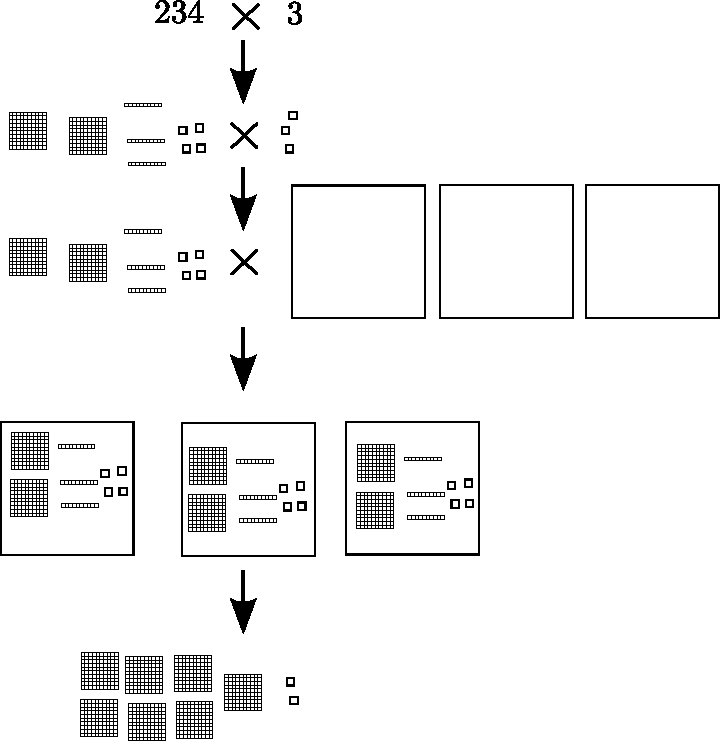
\includegraphics{../graphics/oscarMult.pdf}
\]
Can you explain what is going on? What do you think of his model?
\end{prob}




\begin{prob}
Here is an example of the basic division algorithm:
\[
3\,\begin{tabular}[b]{@{}r@{}r} 
67 &\, R$1$\\ 
\cline{1-1}
\big)\begin{tabular}[t]{@{}l@{}} 202\\ 
18 \\ 
\divrule{0}{2}  ~22 \\
 ~21\\
 \divrule{1}{2}
~~1
\end{tabular}
\end{tabular}
\]
Explain how to model this algorithm with base-ten blocks.
\end{prob}





\newpage
\section{Comparative Arithmetic}\label{A:CA}

\begin{teachingnote}
The point of the activity is that the properties that govern base-ten algorithms carry over to polynomials, but there is no carrying or borrowing.  Ultimately, we want students to see polynomials as numbers in base $x$ and to see base-ten numbers as polynomials in 10.
\end{teachingnote}

\begin{prob} Compute:
\[
\begin{array}{@{}r@{}}
131\\
+122\\ \hline
\end{array}
\qquad\text{and}
\qquad
\begin{array}{@{}r@{}}
x^2+3x+1\\
+x^2+2x+2\\ \hline
\end{array}
\]
Compare, contrast, and describe your experiences.
\end{prob}

\begin{prob} Compute:
\[
\begin{array}{@{}r@{}}
139\\
+122\\ \hline
\end{array}
\qquad\text{and}
\qquad
\begin{array}{@{}r@{}}
x^2+3x+9\\
+x^2+2x+2\\ \hline
\end{array}
\]
Compare, contrast, and describe your experiences. In particular,
discuss how this is different from the first problem.
\end{prob}


\begin{prob} Compute:
\[
\begin{array}{@{}r@{}}
121\\
\times 32\\ \hline
\end{array}
\qquad\text{and}
\qquad
\begin{array}{@{}r@{}}
x^2+2x+1\\
\times~~~3x+2\\ \hline
\end{array}
\]
Compare, contrast, and describe your experiences.
\end{prob}

\begin{prob}
Expand:
\[
(x^2 + 2x + 1)(3x+2)
\]
Compare, contrast, and describe your experiences. In particular, discuss how this problem relates to the one above.
\end{prob}

\fixnote{Need division examples.}


\newpage
\section{Integer Addition and Subtraction}\label{A:integerAddition}
In this activity, we explore various models and strategies for 
making sense of addition and subtraction of integers.  

\subsection*{Useful language}
Addition and subtraction problems arise in situations where we add to, take from, put together, 
take apart, or compare quantities.  

Recall that addition and subtraction facts are related.  For example, if we know that $8+5 = 13$, 
then we also know three related facts:  $5+8=13$, $13-8=5$, and $13-5=8$.  In school mathematics, 
these are often called \emph{fact families}.  

\begin{prob}
What are integers?  Describe some situations in which both positive and negative integers arise.  Use the word ``opposite'' in your descriptions.  
\end{prob}

\subsection*{Red and black chips}
\begin{prob}
In a red-and-black-chip model of the integers, red and black chips each count for $1$, but they are opposites, so that they cancel each other out.  Using language from accounting, suppose black chips are assets and red chips are debts.  We add by putting chips together.  Use red and black chips (or draw the letters $R$ and $B$) to model the following computations.
\begin{enumerate}
\item $(-5)+(-3)$
\item $6+(-4)$.
\item $(-7)+9$
\item $2+(-5)$
\end{enumerate}
\end{prob}

\begin{prob}
In the previous problem, you saw different combinations of red and black chips that had the same numerical value.  
\begin{enumerate}
\item How many ways are there to represent $-3$?  Draw two different representations. 
\item Use the phrase ``zero pairs'' to describe how your two representations are related.  
\end{enumerate}
\end{prob}

\begin{prob}
To subtract in the red-and-black-chip model, we can ``take away'' chips, as you might expect.  When we don't have enough
chips of a particular color, we can always add ``zero pairs.''  Use this idea to model the following subtraction problems: 
\begin{enumerate}
\item $6-8$
\item $4-(-3)$
\item $(-6)-5$
\item $(-3)-(-7)$
\end{enumerate}
\end{prob}

\subsection*{Subtraction as missing addend}
\begin{prob}
To evaluate a subtraction expression, we can solve a related addition equation.  For example, $11-7$ is the solution to $7+\rule[-2pt]{12pt}{.5pt} =11$.  Use this idea to evaluate the subtraction expressions in the previous problem.  
\end{prob}

\subsection*{Subtraction as difference on the number line}
\begin{prob}
Use a number line to reason about $b-a$ by asking how to get from $a$ to $b$:  How far?  And in which direction?   For example, to evaluate $11-7$, we can ask how to get from $7$ to $11$.  We travel $4$ units to the right.  Use this idea to evaluate the subtraction expressions in the previous problems.
\end{prob}

\begin{prob}
How is subtraction different from negation?  
\end{prob}

\begin{prob}
Use what you have learned to explain why $a-(-b)=a+b$.  
\end{prob}

\subsection*{Other Models}  
Use the following models for addition and subtraction of integers.  Each model requires two decisions:  (1) how positive and negative integers are `opposite' in the situation, and (2) how addition and subtraction are `opposite' in a different way.  
\begin{itemize}
\item A postal carrier who brings checks and bills---and who also takes them away.  
\item Walking on an North-South number line, facing either North or South, and walking either forward or backward.  
\end{itemize}



\newpage
\section{Integer Multiplication}\label{A:integerMultiplication}



In this activity, we explore various models and strategies for 
making sense of multiplication of integers.  

\subsection*{Continuing patterns}
\begin{prob}
\begin{enumerate}
\item Continue the following patterns, and explain why it makes sense to continue them in that way.    

\begin{minipage}{0.45\textwidth}
\begin{align*}
4\times 3 &= 12 \\
4\times 2 &= \\
4\times 1 &= \\
4\times 0 &= \\
4\times (-1) &= \\
4\times (-2) &= \\
4\times (-3) &= \\
\end{align*}
\end{minipage}
\begin{minipage}{0.45\textwidth}
\begin{align*}
3\times 6 &= 18 \\
2\times 6 &= \\
1\times 6 &= \\
0\times 6 &= \\
(-1)\times 6 &= \\
(-2)\times 6 &= \\
(-3)\times 6 &= \\
\end{align*}
\end{minipage}
\begin{minipage}{0.45\textwidth}
\begin{align*}
(-7)\times 3 &= -21 \\
(-7)\times 2 &= \\
(-7)\times 1 &= \\
(-7)\times 0 &= \\
(-7)\times (-1) &= \\
(-7)\times (-2) &= \\
(-7)\times (-3) &= \\
\end{align*}
\end{minipage}

\item What rule of multiplication might a student infer from the first pattern? 
\item What rule of multiplication might a student infer from the second pattern?
\item What rule of multiplication might a student infer from the third pattern?
\end{enumerate}
\end{prob}

\subsection*{Using properties of operations}

\begin{prob}
Suppose we \emph{do not know} how to multiply negative numbers but we do know that $4\times 6=24$. We will use this fact and the properties of operations to reason about products involving negative numbers.  
\begin{enumerate}
\item What do we know about $A$ and $B$ if $A+B=0$?  
\item Use the distributive property to show that the expression $4\times 6 + 4\times(-6)$ is equal to $0$.  
Then use that fact to reason about what $4\times(-6)$ should be.  
\item Use the distributive property to show that the expression $4\times (-6) + (-4)\times (-6)$ is equal to $0$.  
Then use that fact to reason about what $(-4)\times(-6)$ should be.  
\end{enumerate}
\end{prob}

\subsection*{Walking on a number line}
\begin{teachingnote}
Again there are two decisions to make: (1) distinguishing positive and negative for the multiplicand; (2) distinguishing positive and negative for the multiplier.
\end{teachingnote}
\begin{prob} 
Matt is a member of the Ohio State University
  Marching Band. Being rather capable, Matt can take $x$ steps of size
  $y$ inches for all integer values of $x$ and $y$.  If $x$ is
  positive it means \textit{face North and take $x$ steps.} If $x$ is
  negative it means \textit{face South and take $|x|$ steps.} If $y$
  is positive it means your step is a \textit{forward step of $y$
    inches.} If $y$ is negative it means your step \textit{is a
    backward step of $|y|$ inches.}
\begin{enumerate}
\item Discuss what the expressions $x \cdot y$ means in this
  context. In particular, what happens if $x = 1$? What if $y=1$?
\item If $x$ and $y$ are both positive, how does this fit with the ``repeated addition'' model of multiplication?    
\item Using the context above and specific numbers, 
demonstrate the general rule:
\[
\text{negative}\cdot \text{positive} = \text{negative}
\]
Clearly explain how your problem shows this.
\item Using the context above and specific numbers, 
demonstrate the general rule:
\[
\text{positive}\cdot \text{negative} = \text{negative}
\]
Clearly explain how your problem shows this.\item Using the context above and specific numbers, 
demonstrate the general rule:
\[
\text{negative}\cdot \text{negative} = \text{positive}
\]
Clearly explain how your problem shows this.
\end{enumerate}
\end{prob}



\newpage
\section{What Can Division Mean?}\label{A:dm}
\fixnote{Connect to even and odd and foreshadow modular arithmetic?}
\fixnote{Typeset this so that students can better see the instructions.  And abbreviate the instructions, perhaps including them below each problem.}  
\fixnote{Use the same numbers more often.  Good examples in my notes.  Fix A.7.5 to round down so that we have the full }

Here are some problems involving division. Someone once told me that
most division problems could be broken into two types:
\begin{enumerate}
\item Those that are asking ``How many groups?''
\item Those that are asking ``How many in one group?''
\end{enumerate}
Let's put this claim to the test. For each of the problems below:
\begin{enumerate}
\item Numerically solve the problem, and explain your reasoning about whether the answer should be a whole number, a quotient and reminder, or a decimal or fraction that is not a whole number.
\item Draw a picture representing the situation and describe actions with objects a student could carry out to solve the problem.
\item Identify whether the problem is asking ``How many groups?'' or ``How many in each group?'' or something else entirely.
\end{enumerate}

\begin{prob}
There are a total of $35$ hard candies. If there are $5$ boxes with an
equal number of candies in each box---and all the candy is accounted
for, then how many candies are in each box? What if you had $39$
candies?
\end{prob}

\begin{prob}
There are a total of $28$ hard candies. If there are $4$ candies in
each box, how many boxes are there? What if you had $34$ candies?
\end{prob}


\begin{prob}
There is a total of 29 gallons of milk to be put in 6 containers.  If
each container holds the same amount of milk and all the milk is
accounted for, how much milk will each container hold?
\end{prob}

 
\begin{prob}
There is a total of 29 gallons of milk to be put in containers holding
6 gallons each.  If all the milk is used, how many containers were
used?
\end{prob}
 
\begin{prob}
If there were 29 kids and each van holds 5 kids, how many vans would
we need for the field trip?
\end{prob}

%\begin{prob}
%Paolo has a total of $48$ outfits (shirts and pants) he can wear. If
%he has $8$ shirts, how many pants does he have?
%\end{prob}



%\begin{prob}
%A chart has $72$ cells and $8$ rows. How many columns does it have?
%\end{prob}

%\begin{prob} 
%A rectangle has a length of $6$ inches and an area of $42$ square
%inches. What is its width?
%\end{prob}

%\begin{prob} 
%Can you think of a division problem that is fundamentally different
%from the problems above?
%\end{prob}

%\begin{prob} 
%In the context of the problems above, what might ``division by zero''
%mean?
%\end{prob}




\newpage
\section{Divisibility Statements}\label{A:divisibilityStatements}

Let $a|b$ mean $b=aq$ for some integer $q$.  (Read $a|b$ as ``$a$ divides $b$''.)  

\begin{prob}
Using the numbers 56 and 7, make some true statements using the notation above and one or more of the words factor, multiple, divisor, and divides.  
\end{prob}

\begin{prob}
Use the definition of \emph{divides} to decide which of the following are true and which are false.  If a statement is true, find $q$ satisfying the definition of divides.  If it is false, give an explanation.  (Hint:  Try to reason about multiplication rather than using your calculator.)
\begin{enumerate}
\item $21|2121$
\item $3|(9\times 41)$
\item $6|(2^4\times 3^2\times 7^3\times 13^5)$
\item $100000|(2^3\times 3^9\times 5^{11}\times 17^8)$
\item $6000|(2^{21}\times 3^7 \times 5^{17}\times 29^5)$
\item $p^3q^5r|(p^5q^{13}r^7s^2t^{27})$
\item $7|(5\times 21 + 14)$
\end{enumerate}
\end{prob}

\fixnote{Need some easier examples above.  Below, we need at least one that isn't true.  Use converses of some of these?}

\begin{prob}
If $a|b$ and $a|c$ does $a|(bc)$?  Explain. 
\end{prob}

\begin{prob}
If $a|b$ and $a|c$ does $a|(b+c)$?  Explain.  
\end{prob}

\begin{prob}
If $a|(b+c)$ and $a|c$ does $a|b$?  Explain.  
\end{prob}

\begin{prob}
Suppose that $$(3^5\cdot 7^9\cdot 11^x\cdot 13^y)|(3^a\cdot 7^b\cdot 11^{19}\cdot 13^7)$$
What values of $a$, $b$, $x$, and $y$ make true statements? 
\end{prob}


\newpage
\section{Hall of Shoes}\label{A:Hall}
  
\begin{prob}  
\textit{Incognito's Hall of Shoes} is a shoe store that just
  opened in Myrtle Beach, South Carolina. At the moment, they have 100
  pairs of shoes in stock. At their grand opening 100 customers showed
  up. The first customer tried on every pair of shoes, the second
  customer tried on every 2nd pair, the third customer tried on every
  3rd pair, and so on until the 100th customer, who only tried on the
  last pair of shoes.
\begin{enumerate}
\item Which shoes were tried on by only 1 customer?
\item Which shoes were tried on by exactly 2 customers?
\item Which shoes were tried on by exactly 3 customers?
\item Which shoes were tried on by exactly 4 customers?
\item How many customers tried on the 45th pair?  
\item How many customers tried on the 81st pair?  
\item Challenge:  Which shoes were tried on by the most customers?  
\end{enumerate}
In each case, explain your reasoning.
\end{prob}

\begin{prob}
Which pairs of shoes were tried on by both 
\begin{enumerate}
\item customers 3 and 5?
\item customers 6 and 8?
\item customers 12 and 30?
\item customers 7 and 13?
\item customers $a$ and $b$?  
\end{enumerate}
\end{prob}

\begin{prob}
Which customers tried on both 
\begin{enumerate}
\item pairs 24 and 36?
\item pairs 30 and 60?
\item pairs 42 and 12?
\item pairs 28 and 15?
\item pairs $a$ and $b$?  
\end{enumerate}
\end{prob}




\newpage
\section{Sieving It All Out}\label{A:Sie}
\begin{prob}  
\textit{Incognito's Hall of Shoes} is a shoe store that just
  opened in Myrtle Beach, South Carolina. At the moment, they have 100
  pairs of shoes in stock. At their grand opening 100 customers showed
  up. The first customer tried on every pair of shoes, the second
  customer tried on every 2nd pair, the third customer tried on every
  3rd pair, and so on until the 100th customer, who only tried on the
  last pair of shoes.
\begin{enumerate}
\item Which shoes were tried on by only 1 customer?
\item Which shoes were tried on by exactly 2 customers?
\item Which shoes were tried on by exactly 3 customers?
\item Which shoes were tried on by the most customers?
\item How many customers tried on the 45th pair?  
\item How many customers tried on the 81st pair?  
\end{enumerate}
In each case, explain your reasoning.
\end{prob}

\begin{prob}
Which pairs of shoes were tried on by both 
\begin{enumerate}
\item customers 3 and 5?
\item customers 6 and 8?
\item customers 12 and 30?
\item customers 7 and 13?
\end{enumerate}
\end{prob}

\begin{prob}
Which customers tried on both 
\begin{enumerate}
\item pairs 24 and 36?
\item pairs 30 and 60?
\item pairs 42 and 12?
\item pairs 28 and 15?
\end{enumerate}
\end{prob}


\newpage


\begin{prob} 
Use ideas from Incognito's Hall of Shoes to find all the primes from $1$ to $120$ \textit{without}
doing any division.  Systematically try to circle numbers that are prime and 
cross out numbers that are not prime.  As a jesture of friendship, here are the numbers from $1$ to $120$.
\[
\begin{tabular}{r r r r r r r r r r}

  1 &   2 &   3 &   4 &   5 &   6 &   7 &   8 &   9 &  10\\
  \\
 11 &  12 &  13 &  14 &  15 &  16 &  17 &  18 &  19 &  20\\
 \\
 21 &  22 &  23 &  24 &  25 &  26 &  27 &  28 &  29 &  30\\
 \\
 31 &  32 &  33 &  34 &  35 &  36 &  37 &  38 &  39 &  40\\
 \\
 41 &  42 &  43 &  44 &  45 &  46 &  47 &  48 &  49 &  50\\
 \\
 51 &  52 &  53 &  54 &  55 &  56 &  57 &  58 &  59 &  60\\
 \\
 61 &  62 &  63 &  64 &  65 &  66 &  67 &  68 &  69 &  70\\
 \\
 71 &  72 &  73 &  74 &  75 &  76 &  77 &  78 &  79 &  80\\
 \\
 81 &  82 &  83 &  84 &  85 &  86 &  87 &  88 &  89 &  90\\
 \\
 91 &  92 &  93 &  94 &  95 &  96 &  97 &  98 &  99 & 100\\
 \\
101 & 102 & 103 & 104 & 105 & 106 & 107 & 108 & 109 & 110\\
\\
111 & 112 & 113 & 114 & 115 & 116 & 117 & 118 & 119 & 120\\
\end{tabular}
\]

Describe your method.  
\end{prob}

\begin{prob}
In the previous problem, after circling a new prime, what was the first number crossed out with that prime?  What was the biggest prime for which you crossed out at least one multiple?
\end{prob}


\begin{prob}
Find all of the prime factors of 1008. How can you be sure you've
found them all?
\end{prob}


\newpage
\section{There's Always Another Prime}\label{A:Pr}

We'll start off with easy questions, then move to harder ones.

\begin{prob}
Use the Division Theorem to explain why $2$ does not divide $2+1$.
\end{prob}

\begin{prob}
Use the Division Theorem to explain why neither $2$ nor $3$ divides
$2\cdot 3+1$.
\end{prob}

\begin{prob}
Use the Division Theorem to explain why neither $2$ nor $3$ nor $5$ divides
$2\cdot 3\cdot 5+1$.
\end{prob}

\begin{prob} 
Let $p_1,\dots, p_n$ be the first $n$ primes. Do any of these primes divide 
\[
p_1p_2\cdots p_n + 1?
\]
Explain your reasoning.
\end{prob}


\begin{prob} 
Suppose there were only a finite number of primes, say there were only
$n$ of them. Call them $p_1,\dots, p_n$. Could any of them divide
\[
p_1p_2\cdots p_n + 1?
\]
what does that mean? Can there really only be a finite number of
primes?
\end{prob}



\begin{prob} 
Consider the following:
\[
2\cdot 3\cdot 5\cdot 7 \cdot 11\cdot 13 + 1 = 59\cdot 509
\] 
Does this contradict our work above? If so, explain why. If not, explain
why not.
\end{prob}




\newpage
\section{There Are Many Factors to Consider}\label{A:CF}

\fixnote{Revise.  List all factors of several numbers.  Need an example where being systematic by consecutive numbers (rather than by using prime factorization) is inefficient.
List all the factors of 60 with their prime factorization.  
Insert the activity borrowed from 1125 about using the prime factorizations to determine whether one number is a factor of another.   
}  

\begin{prob} How many factors does the integer $60$ have?
\end{prob}

\begin{prob}
Consider the following diagram:
\[
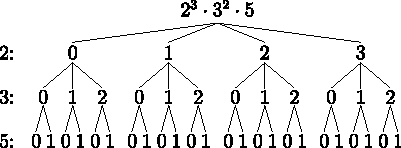
\includegraphics{../graphics/treeDia.pdf}
\]
What is going on in this diagram? What do the numbers represent? How
does it help you count the number of factors of $2^3\cdot 3^2 \cdot
5$?
\end{prob}

\begin{prob}
Make a similar diagram for $60$.
\end{prob}

\begin{prob} 
Can you devise a method for computing the number of factors that a
number has? Explain why your method works.
\end{prob}

\begin{prob} How many factors does $735$ have?
\end{prob}

\begin{prob} 
If $p$ is a prime number, how many factors does $p^n$ have?
\end{prob}

\begin{prob} 
If $p$ and $q$ are both prime numbers, how many factors does $p^nq^m$
have?
\end{prob}

\begin{prob} Which integers between $0$ and $100$ have the most factors?         
\end{prob}


\newpage
\section{Why Does It Work?}\label{A:GCDwork}

The Euclidean Algorithm\index{Euclidean Algorithm} is pretty
neat. Let's see if we can figure out \textbf{why} it works. As a gesture of friendship, I'll compute $\gcd(351,153)$:
\begin{align*}
351 &= \boldsymbol{153}\cdot 2 + \boldsymbol{45}\\ 
\boldsymbol{153} &= \boldsymbol{45}\cdot 3 + \boldsymbol{18}\\
\boldsymbol{45} &= \boldsymbol{18}\cdot 2 + \fbox{$\boldsymbol{9}$}\\
18 &= 9\cdot 2 + 0 \qquad \fbox{$\therefore \gcd(351,153) = 9$}
\end{align*}

Let's look at this line-by-line.

\paragraph{The First Line}
\begin{prob}
Since $351 = 153\cdot 2 + 45$, explain why $\gcd(153,45)$ divides $351$.
\end{prob}

\begin{prob}
Since $351 = 153\cdot 2 + 45$, explain why $\gcd(351,153)$ divides $45$.
\end{prob}

\begin{prob}
Since $351 = 153\cdot 2 + 45$, explain why $\gcd(351,153) = \gcd(153,45)$.
\end{prob}


\paragraph{The Second Line}
\begin{prob}
Since $153 = 45\cdot 3 + 18$, explain why $\gcd(45,18)$ divides $153$.
\end{prob}

\begin{prob}
Since $153 = 45\cdot 3 + 18$, explain why $\gcd(153,45)$ divides $18$.
\end{prob}

\begin{prob}
Since $153 = 45\cdot 3 + 18$, explain why $\gcd(153,45) = \gcd(45,18)$.
\end{prob}


\paragraph{The Third Line}
\begin{prob}
Since $45 = 18\cdot 2 + 9$, explain why $\gcd(18,9)$ divides $45$.
\end{prob}

\begin{prob}
Since $45 = 18\cdot 2 + 9$, explain why $\gcd(45,18)$ divides $9$.
\end{prob}

\begin{prob}
Since $45 = 18\cdot 2 + 9$, explain why $\gcd(45,18) = \gcd(18,9)$.
\end{prob}


\paragraph{The Final Line}

\begin{prob}
Why are we done? How do you know that the Euclidean Algorithm
will \textbf{always} terminate?
\end{prob}

\fixnote{New question:  What does the final line look like when the GCD is 1?}  

\newpage
\section{Prome Factorization}\label{A:Prome}

\begin{teachingnote}
In the course, we first assume Euclid's Lemma and use it to prove the Fundamental Theorem of Arithmetic (FTA).  Here both Euclid's Lemma and the FTA fail.
\end{teachingnote}

Let's consider a crazy set of numbers---all multiples of $3$. Let's
use the symbol $3\Z$ to denote the set consisting of all multiples of
$3$. As a gesture of friendship, I have written down the first $100$
nonnegative integers in $3\Z$:

\[
\begin{array}{cccccccccc}
0   & 3   & 6   & 9   & 12  & 15  & 18  & 21  & 24  & 27  \\
\\
30  & 33  & 36  & 39  & 42  & 45  & 48  & 51  & 54  & 57  \\
\\
60  & 63  & 66  & 69  & 72  & 75  & 78  & 81  & 84  & 87  \\
\\
90  & 93  & 96  & 99  & 102 & 105 & 108 & 111 & 114 & 117 \\
\\
120 & 123 & 126 & 129 & 132 & 135 & 138 & 141 & 144 & 147 \\
\\
150 & 153 & 156 & 159 & 162 & 165 & 168 & 171 & 174 & 177 \\
\\
180 & 183 & 186 & 189 & 192 & 195 & 198 & 201 & 204 & 207 \\
\\
210 & 213 & 216 & 219 & 222 & 225 & 228 & 231 & 234 & 237 \\
\\
240 & 243 & 246 & 249 & 252 & 255 & 258 & 261 & 264 & 267 \\
\\
270 & 273 & 276 & 279 & 282 & 285 & 288 & 291 & 294 & 297
\end{array}
\]



\begin{prob}
Given any two integers in $3\Z$, will their sum be in $3\Z$? Explain
your reasoning.
\end{prob}

\begin{prob}
Given any two integers in $3\Z$, will their difference be in $3\Z$?
Explain your reasoning.
\end{prob}

\begin{prob}
Given any two integers in $3\Z$, will their product be in $3\Z$?
Explain your reasoning.
\end{prob}

\begin{prob}
Given any two integers in $3\Z$, will their quotient be in $3\Z$?
Explain your reasoning.
\end{prob}

\begin{definition}
Call a positive integer \textbf{prome} in $3\Z$ if it cannot be
expressed as the product of two integers \textit{both} in $3\Z$.
\end{definition}

As an example, I tell you that $6$ is prome number in $3\Z$. You may
object because $6 = 2\cdot 3$, but remember---$2$ is not in $3\Z$!


\begin{prob}
List some of the prome numbers less than $297$.  Hint:  What numbers in $3\Z$ \emph{can} be expressed as a product of two integers \emph{both} in $3\Z$?  
\end{prob}

\begin{prob}
Can you give some sort of algebraic characterization of prome numbers
in $3\Z$? 
\end{prob}

\begin{prob}
Can you find numbers that factor completely into prome numbers in
\textit{two} different ways? How many can you find?
\end{prob}






\newpage
\section{Picture Models for Equivalent Fractions}\label{A:EF}

\begin{teachingnote}

Step 1.  Use the first problem (use paper to show 3/8) to generate the meaning of fraction from the Common Core State Standards:  

\begin{quote}
3.NF.1. Understand a fraction $1/b$ as the quantity formed by $1$ part when a
whole is partitioned into $b$ equal parts; understand a fraction $a/b$ as
the quantity formed by $a$ parts of size $1/b$.

Source:  \url{http://www.corestandards.org/Math/Content/3/NF/A/1/}
\end{quote}


The code 3.NF.1 means ``third grade, number and operations--fractions, standard 1.''  These standards are written to be read by teachers, not students.

Step 2.  Introduce the formal definition of rational number and the set of rational numbers, as in the beginning of section 2.4.  

A rational number can be represented as $a/b$ with integers $a$ and $b$, where $b$ is not $0$.  

Distinguish fraction (a representation) from rational number, highlighting the phrase ``can be'' in the definition.  Have students generate fractions that are not rational numbers as well as rational numbers not represented as fractions.  

Introduce the letter $\Q$ (usually in ``black-board bold'' font) to denote the set of all rational numbers. 

Step 3.  Complete Activity A.16.  The point is to use the meaning of fractions above to explain why fractions are equivalent.  And the approach is ``reasoning generally with specific numbers.'' 

A.16.2.  For $2/3 = 4/6$, some students will be tempted to draw 2/3, draw 4/6 and then say, ``See!''  With this method, it is not clear why the pieces should line up.  Much better to use 2/3 to create 4/6 by cutting each of the thirds into two equal pieces.  

A.16.3.  For $3/6 = 2/4$, some students will be tempted to say ``Because they both equal 1/2.''  To explain why the pieces will have to line up, it is clearer (and more general) to go through a common denominator, such as 12ths or 24ths.  
 
A.16.4.  To show that $a/b = c/d$, generalize the approach from the previous problem:  Thinking of the common denominator $bd$, cut the $a/b$ parts each into $d$ parts.  Then we have $ad$ parts of size $1/(bd)$.  Cut the $c/d$ parts each into $b$ parts.  Then we have $cb$ parts of size $1/(db)$.  For the two fractions to be equal, the $ad$ parts of size $1/(bd)$ must be equal to the $cb$ parts of size $1/(db)$.  

A.16.5.  In the picture from A.16.4, because the parts are the same size (i.e., $1/(bd)$), it must follow that $ad = bc$.  (Argue both directions:  if the fractions are equal, then $ad = bc$;  if $ad = bc$, then the fractions must be equal.)  
\end{teachingnote}

\begin{prob}
Get out a piece of paper and show $\dfrac{3}{8}$.  Explain how you know.  
\end{prob}

\begin{prob}
Compare the following fractions.  Explain how you know:
\begin{enumerate}
\item $\frac{3}{5} \qquad \frac{4}{5}$
\item $\frac{3}{7} \qquad \frac{3}{8}$
\item $\frac{3}{7} \qquad \frac{5}{9}$
\item $\frac{6}{7} \qquad \frac{7}{8}$
\item $\frac{12}{11} \qquad \frac{13}{14}$
\end{enumerate}
\begin{teachingnote}
In the above comparison problems, highlight common denominator and common numerator strategies.  Also highlight comparing to benchmarks such as $1/2$ or $1$. 
\end{teachingnote}
\end{prob}

\begin{prob} 
Draw pictures to explain why:
\[
\frac{2}{3} = \frac{4}{6}
\]
Explain how your pictures show this.
\end{prob}


\begin{prob} 
Draw pictures to explain why:
\[
\frac{3}{6} = \frac{2}{4}
\]
Explain how your pictures show this.
\end{prob}



\begin{prob} 
Given equivalent fractions with $0< a\le b$ and $0 < c\le d$:
\[
\frac{a}{b} = \frac{c}{d}
\]
Give a procedure for representing this equation with pictures.
\end{prob}


\begin{prob} 
Explain, without cross-multiplication, why if $0< a\le b$ and $0 < c\le d$:
\[
\frac{a}{b} = \frac{c}{d}\qquad \text{if and only if}\qquad ad = bc
\]
Feel free to use pictures as part of your explanation.
\end{prob}


\newpage
\section{Picture Models for Fraction Operations}\label{A:FO}
\begin{prob} 
Draw pictures that model:
\[
\frac{1}{5} + \frac{2}{5} = \frac{3}{5}
\]
Explain how your pictures show this. Write a story problem whose
solution is given by the expression above.
\end{prob}

\begin{prob} 
Draw pictures that model:
\[
\frac{2}{3} + \frac{1}{4} = \frac{11}{12}
\]
Explain how your pictures model this equation. Be sure to carefully
explain how common denominators are represented in your
pictures. Write a story problem whose solution is given by the
expression above.
\end{prob}

\begin{prob} 
Given $0<a\le b$ and $0<c\le d$, explain how to draw pictures
that model the sum:
\[
\frac{a}{b} + \frac{c}{d}
\]
Use pictures to find this sum and carefully explain how common
denominators are represented in your pictures.
\end{prob}

\fixnote{Need some questions about comparing fractions using common denominators, common numerators, benchmark fractions as well as some fractions greater than 1.  See 2016 notes, p. 153.}

% The following problems have been replaced by a new activity about fraction multiplication
%
%\begin{prob} 
%Given positive integers $a$ and $b$, explain how to draw pictures that
%model the product $a\cdot b$---give an example of your process.
%\end{prob}
%
%\begin{prob} 
%Draw pictures that model:
%\[
%\frac{4}{5} \cdot \frac{2}{3} = \frac{8}{15}
%\]
%Explain how your pictures model this equation. Write a story problem
%whose solution is given by the expression above. Does your story work with 
%\[
%\frac{7}{5} \cdot \frac{2}{3} = \frac{14}{15}?
%\]
%\end{prob}
%
%\begin{prob} 
%Given $0<a\le b$ and $0<c\le d$, explain how to draw pictures
%that model the product:
%\[
%\frac{a}{b} \cdot \frac{c}{d}
%\]
%Use pictures to find this product and explain how this product is shown
%in your pictures---give an example of your process.
%\end{prob}


\newpage
\section{Fraction Multiplication}\label{A:fractionMultiplication}

\begin{prob}
Suppose $x$ and $y$ are counting numbers.  
\begin{enumerate}
\item What is our convention for the meaning of $xy$ as repeated addition?  
\item In our convention for the meaning of the product $xy$, which letter describes 
\emph{how many groups} and which letter describes \emph{how many in one group}? 
\item In the product $xy$, the $x$ is called the \emph{multiplier} and $y$ is called the \emph{multiplicand}.  
Use these words to describe the meaning of $xy$ as repeated addition. 
\end{enumerate}
\end{prob}

\vspace{1in}

\begin{prob}
In the Common Core State Standards, fractions and fraction operations are built from \emph{unit fractions}, which are fractions with a $1$ in the numerator.  The meaning of a fraction $\frac{a}{b}$ involves three steps: (1) determining the whole; (2) describing the meaning of $\frac{1}{b}$; and (3) describe the meaning of the fraction $\frac{a}{b}$.  Use pictures to illustrate these three steps for the fraction
$\frac{3}{5}$.  
\end{prob}

\vspace{1in}

\begin{prob}
Now we combine the ideas from the previous two problems to describe meanings for simple multiplication of fractions.  
\begin{enumerate}
\item Without computing the result, describe the meaning of the product $5 \times \frac{1}{3}$.
\item Without computing the result, describe the meaning of the product $\frac{1}{3}\times 5$.
\item Without using the commutativity of multiplication (which we have not established for fractions), 
use these meanings and pictures to explain what the products should be. 
\end{enumerate}
\end{prob}

\vspace{1in}

\subsection*{Area Models}
\begin{prob}
Beginning with a unit square, use an area model to illustrate the following:  
\begin{enumerate}
\item $\frac{1}{3}\times \frac{1}{4}$ 
\item $\frac{7}{3}\times \frac{5}{4}$
\end{enumerate}
\end{prob}

\vspace{1.5in}
\
\begin{prob}
When computing $2\frac{1}{3}\times 3\frac{2}{5}$, Byron says that the answer is $6\frac{2}{15}$.  
\begin{enumerate}
\item Explain Byron's method. 
\item How do you know that he is incorrect?  
\item Use what is right about his method to show what he is missing. 
\end{enumerate}
\end{prob}


\newpage
\section{Flour Power}\label{A:FlourPower}

\begin{prob} 
Suppose a cookie recipe calls for $2$ cups of flour. If you have $6$
cups of flour total, how many batches of cookies can you make?
\begin{enumerate}
\item Draw a picture representing the situation, and use pictures to solve the problem.
\item Identify whether the problem is asking ``How many groups?'' or ``How many in one group?'' or something else entirely.
\item You find another recipe that calls for $1\frac{1}{2}$ cups per batch. If you have $6$ cups of flour, how many batches of these cookies can you make?  Again use pictures to solve the problem.
\item Somebody once told you that ``to divide fractions, you invert and
multiply.'' Discuss how this rule is manifested in this problem.
\end{enumerate}
\end{prob}

\begin{prob} 
You have $2$ snazzy stainless steel containers (both the same size), which hold a total of
$6$ cups of flour. How many cups of flour does $1$ container hold?
\begin{enumerate}
\item Draw a picture representing the situation, and use pictures to solve the problem.
\item Identify whether the problem is asking ``How many groups?'' or ``How many in one group?'' or something else entirely.
\item It turned out that the 6 cups of flour filled exactly $1\frac{1}{2}$ of your containers.  How many cups of flour does $1$ container hold?  Again use pictures to solve the problem.
\item Somebody once told you that ``to divide fractions, you invert and
multiply.'' Discuss how this rule is manifested in this problem.
\end{enumerate}
\end{prob}


%\begin{prob} 
%Now you have $3$ beautiful decorative bowls, which hold a total of
%$1/2$ cup of flour. How many cups of flour does $1$ decorative bowl
%hold?
%\begin{enumerate}
%\item Draw a picture representing the situation, and use your picture to solve the problem.
%\item Identify whether the problem is asking ``How many groups?'' or ``How many in one group?'' or something else entirely.
%\item Somebody once told you that ``to divide fractions, you invert and
%multiply.'' Discuss how this rule is manifested in this problem.
%\end{enumerate}
%\end{prob}
%


\newpage
\section{Picture Yourself Dividing}


We want to understand how to visualize 
\[
\frac{a}{b} \div \frac{c}{d}
\]
Let's see if we can ease into this like a cold swimming pool.

\begin{prob}
Draw a picture that shows how to compute:
\[
6\div 3
\]
Explain how your picture could be redrawn for other similar
numbers. Write two story problems solved by this expression, one
asking for ``how many groups'' and the other asking for ``how many in
each group.''
\end{prob}

\begin{prob}
Try to use a similar process to the one you used in the first problem
to draw a picture that shows how to compute:
\[
\frac{1}{4} \div 3
\]
Explain how your picture could be redrawn for other similar numbers.
Write two story problems solved by this expression, one asking for
``how many groups'' and the other asking for ``how many in each
group.''
\end{prob}


\begin{prob}
Try to use a similar process to the one you used in the first two problems
to draw a picture that shows how to compute:
\[
3 \div \frac{1}{4}
\]
Explain how your picture could be redrawn for other similar numbers.
Write two story problems solved by this expression, one asking for
``how many groups'' and the other asking for ``how many in each
group.''
\end{prob}

\fixnote{Also incorporate $1\frac{3}{4}\div \frac{1}{2}$}

\begin{prob}
Try to use a similar process to the one you used in the first three problems
to draw a picture that shows how to compute:
\[
\frac{7}{5} \div \frac{3}{4}
\]
Explain how your picture could be redrawn for other similar numbers.
Write two story problems solved by this expression, one asking for
``how many groups'' and the other asking for ``how many in each
group.''
\end{prob}

\begin{prob}
Explain how to draw pictures to visualize:
\[
\frac{a}{b} \div \frac{c}{d}
\]
\end{prob}

\begin{prob}
Use pictures to explain why:
\[
\frac{a}{b} \div \frac{c}{d} = \frac{a}{b} \cdot \frac{d}{c}
\]
\end{prob}


\newpage
\section{Cross Something-ing}


\begin{prob} 
What might someone call the following statements:
\begin{enumerate}
\item $\dfrac{a}{b} = \dfrac{c}{d} \Rightarrow ad = bc$
\item $\dfrac{a}{b}\cdot \dfrac{b}{c} = \dfrac{a}{c}$
\item $\dfrac{a}{b} +\dfrac{c}{d} = \dfrac{ad+bc}{bd}$
\item $ad < bc \Rightarrow \dfrac{a}{b} < \dfrac{c}{d}$
\item $ad < bc \Rightarrow \dfrac{c}{d} < \dfrac{a}{b}$
\end{enumerate}
\end{prob}

\begin{prob}
Which of the above statements are true? What specific name might you
use to describe them?
\end{prob}

\begin{prob} 
Use pictures to help explain why the true statements above are true
and give counterexamples showing that the false statements are false.
\end{prob}


\begin{prob} 
Can you think of other statements that should be grouped with those
above?
\end{prob}

\begin{prob}
If mathematics is a subject where you should strive to ``say what you
mean and mean what you say,'' what issue might arise with
cross-multiplication?
\end{prob}



\newpage
\section{Hundredths Grids for Rational Numbers}\label{A:hundredthsGrids}

%% Use tikz to generate the graphics

When a $10\times 10$ square is taken to be $1$ whole, it can be used as a ``hundredths grid'' 
to represent fractions and decimals between $0$ and $1$.\margincomment{For example, one of the grids below 
is shaded to represent $\frac{21}{100}$.}

\begin{prob}
Shade the hundredths grids to show each of the following fractions.  Then use your shading to determine a decimal equivalent for each fraction.  
\begin{center}
\hfill (a) $\frac{3}{20}$ \hfill (b) $\frac{1}{8}$ \hfill (c) $\frac{1}{6}$ \hfill (d) $\frac{7}{12}$ \hfill
\end{center}

\begin{fullwidth}\em\em\quad
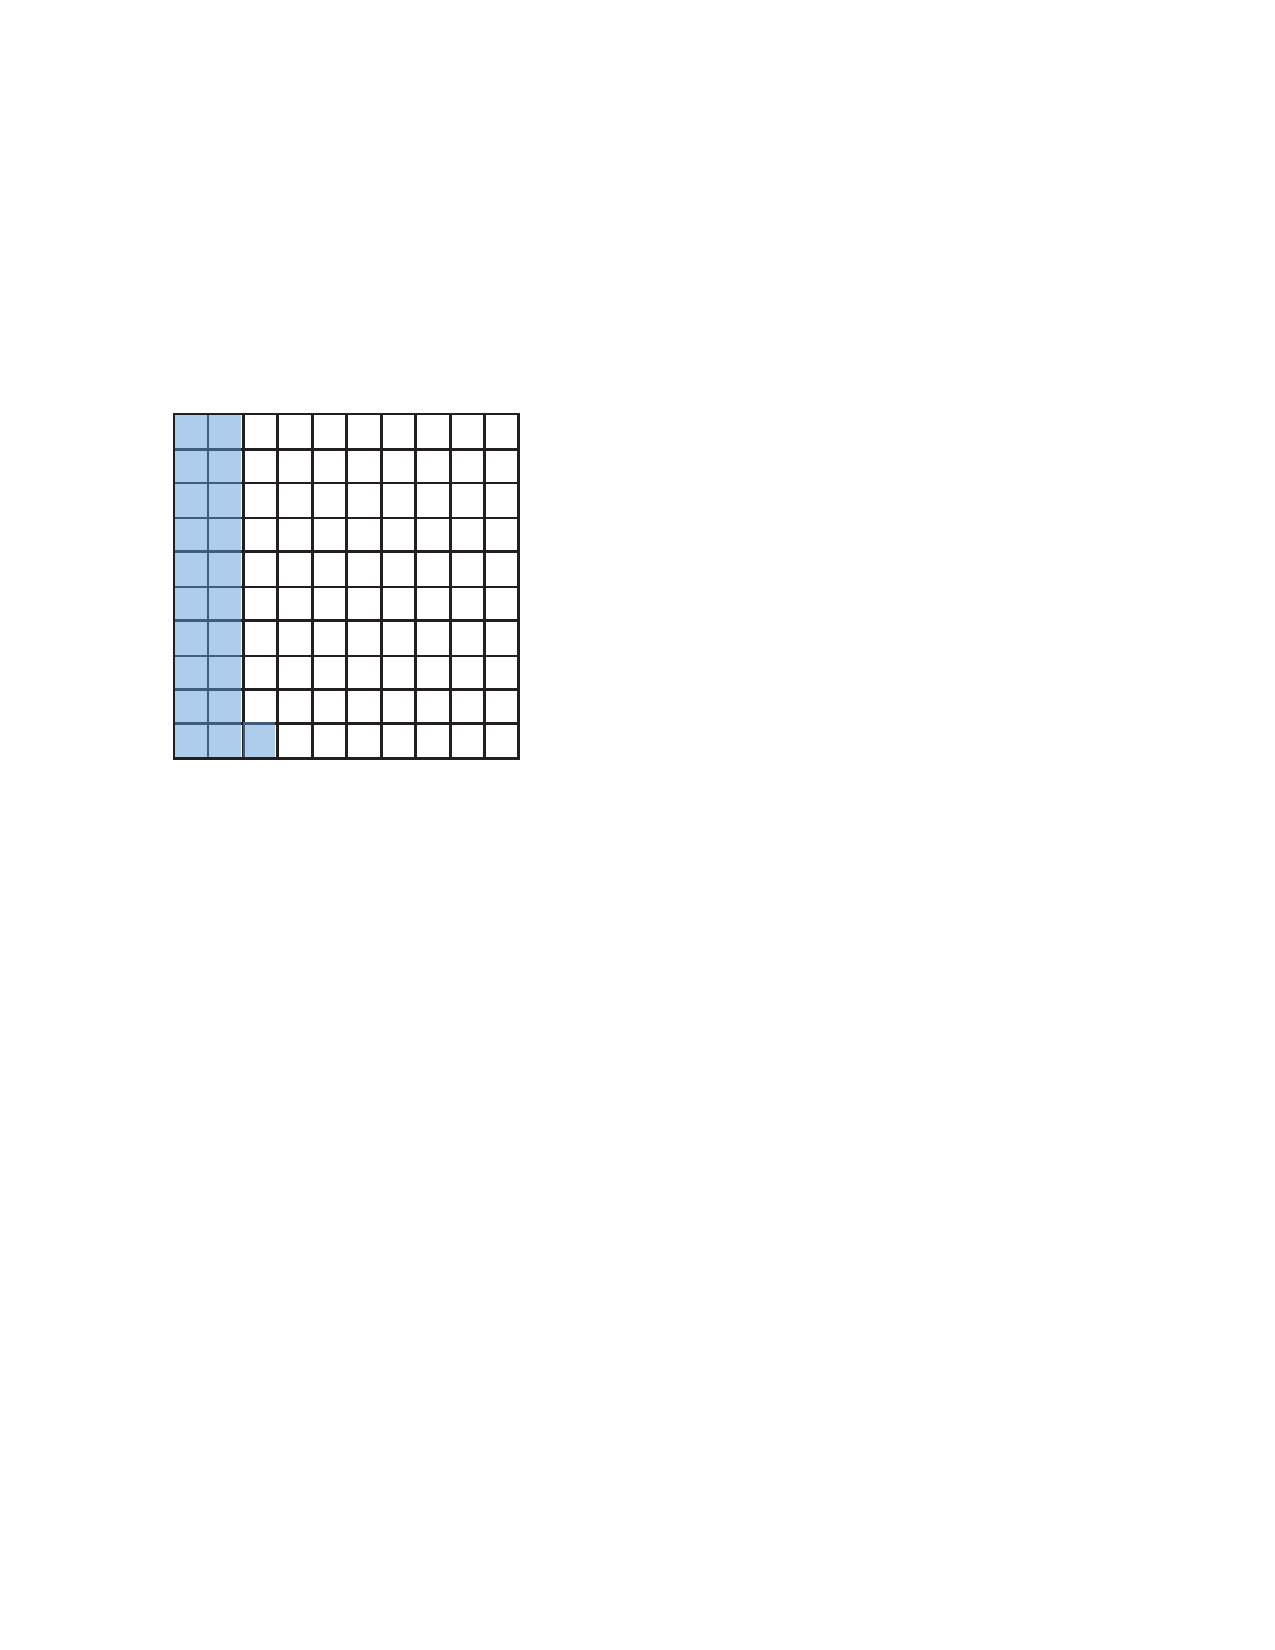
\includegraphics{../graphics/hundredthsGridSample}\quad
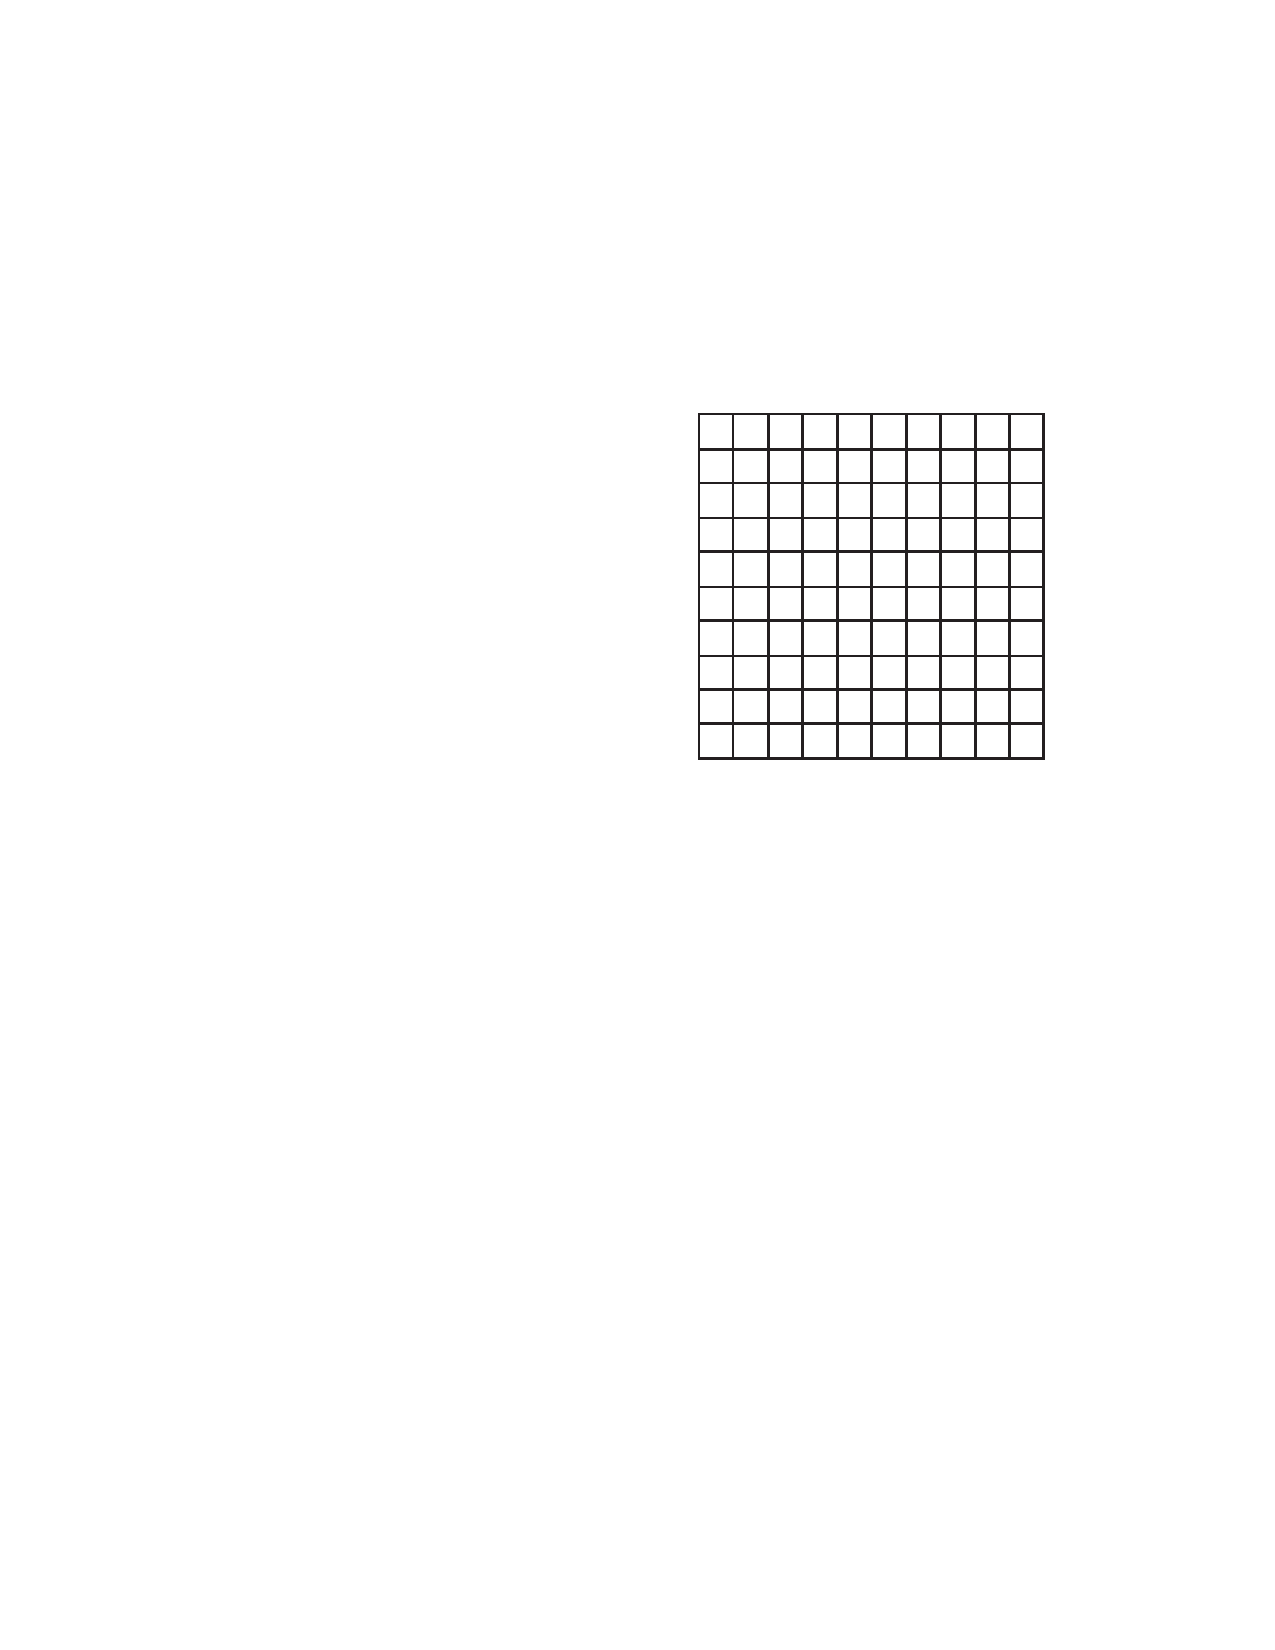
\includegraphics{../graphics/hundredthsGrid}\quad
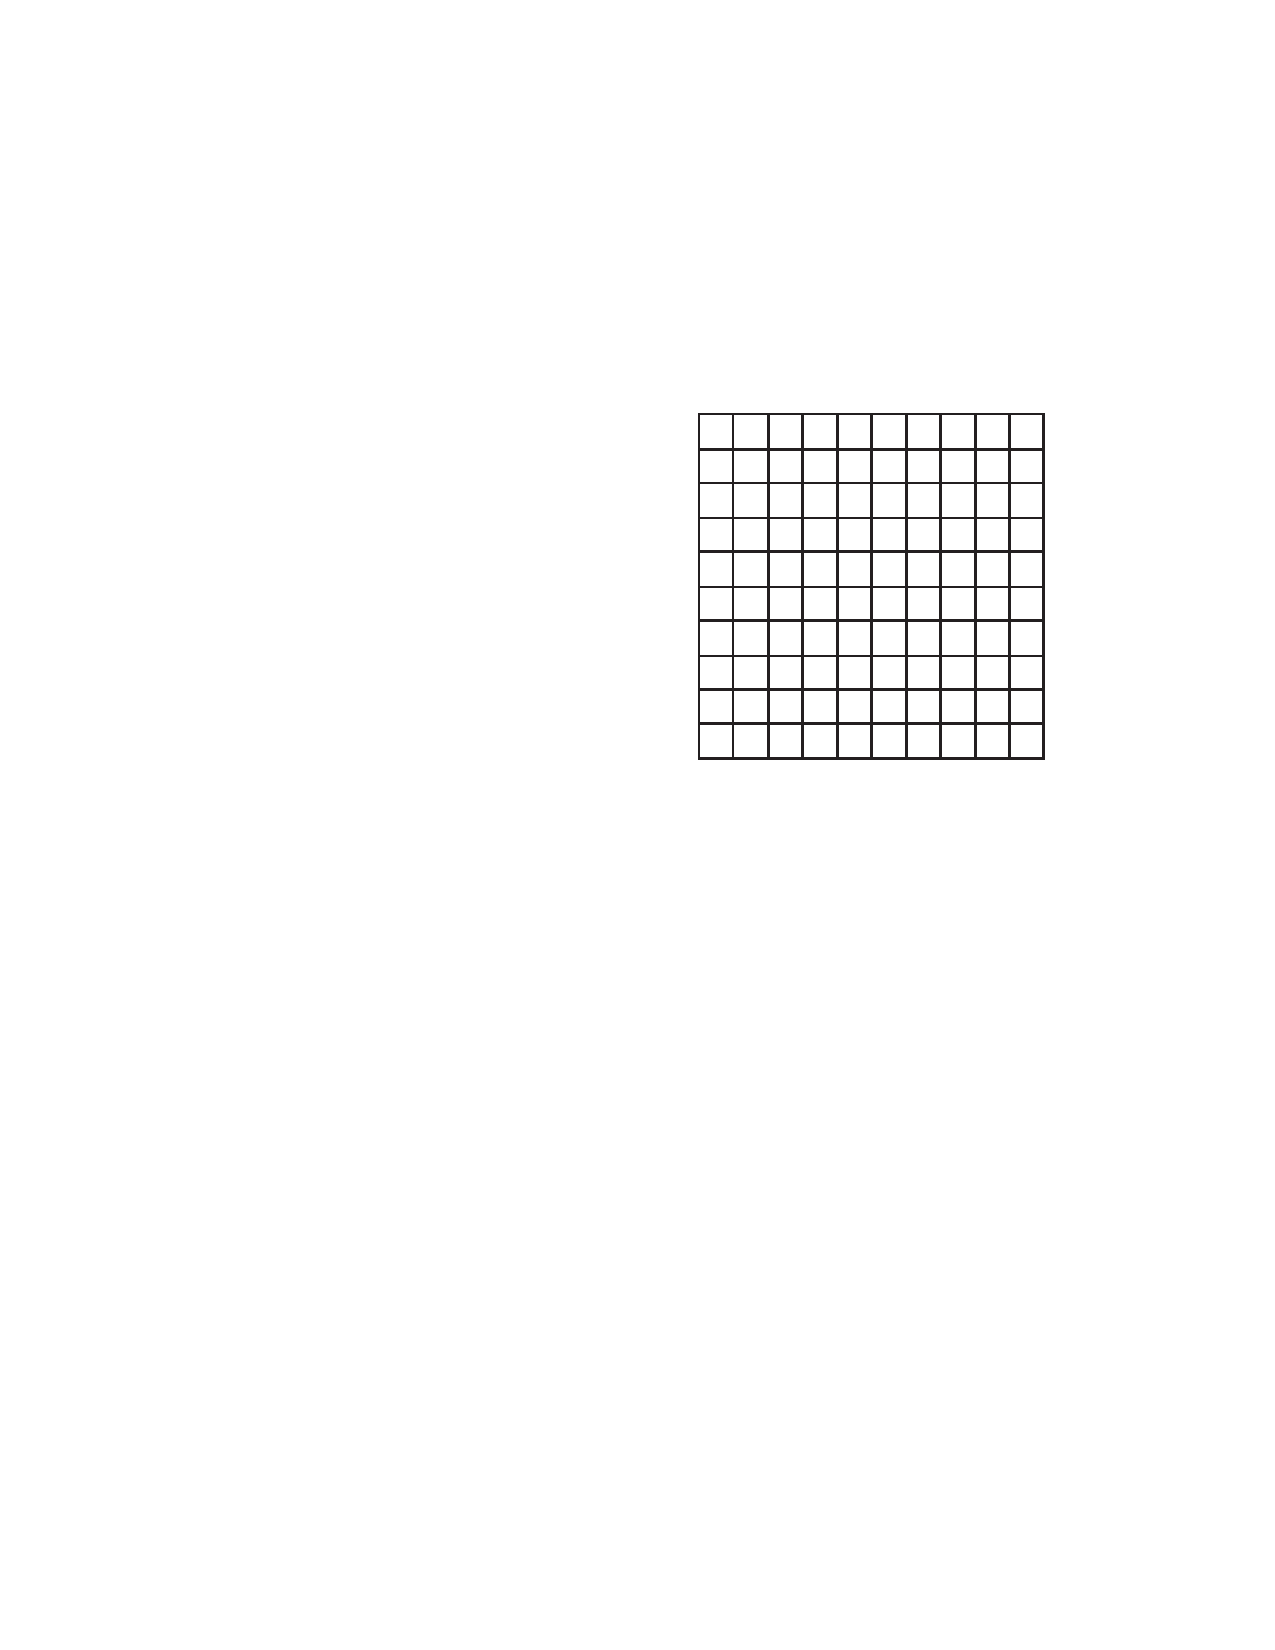
\includegraphics{../graphics/hundredthsGrid}\\

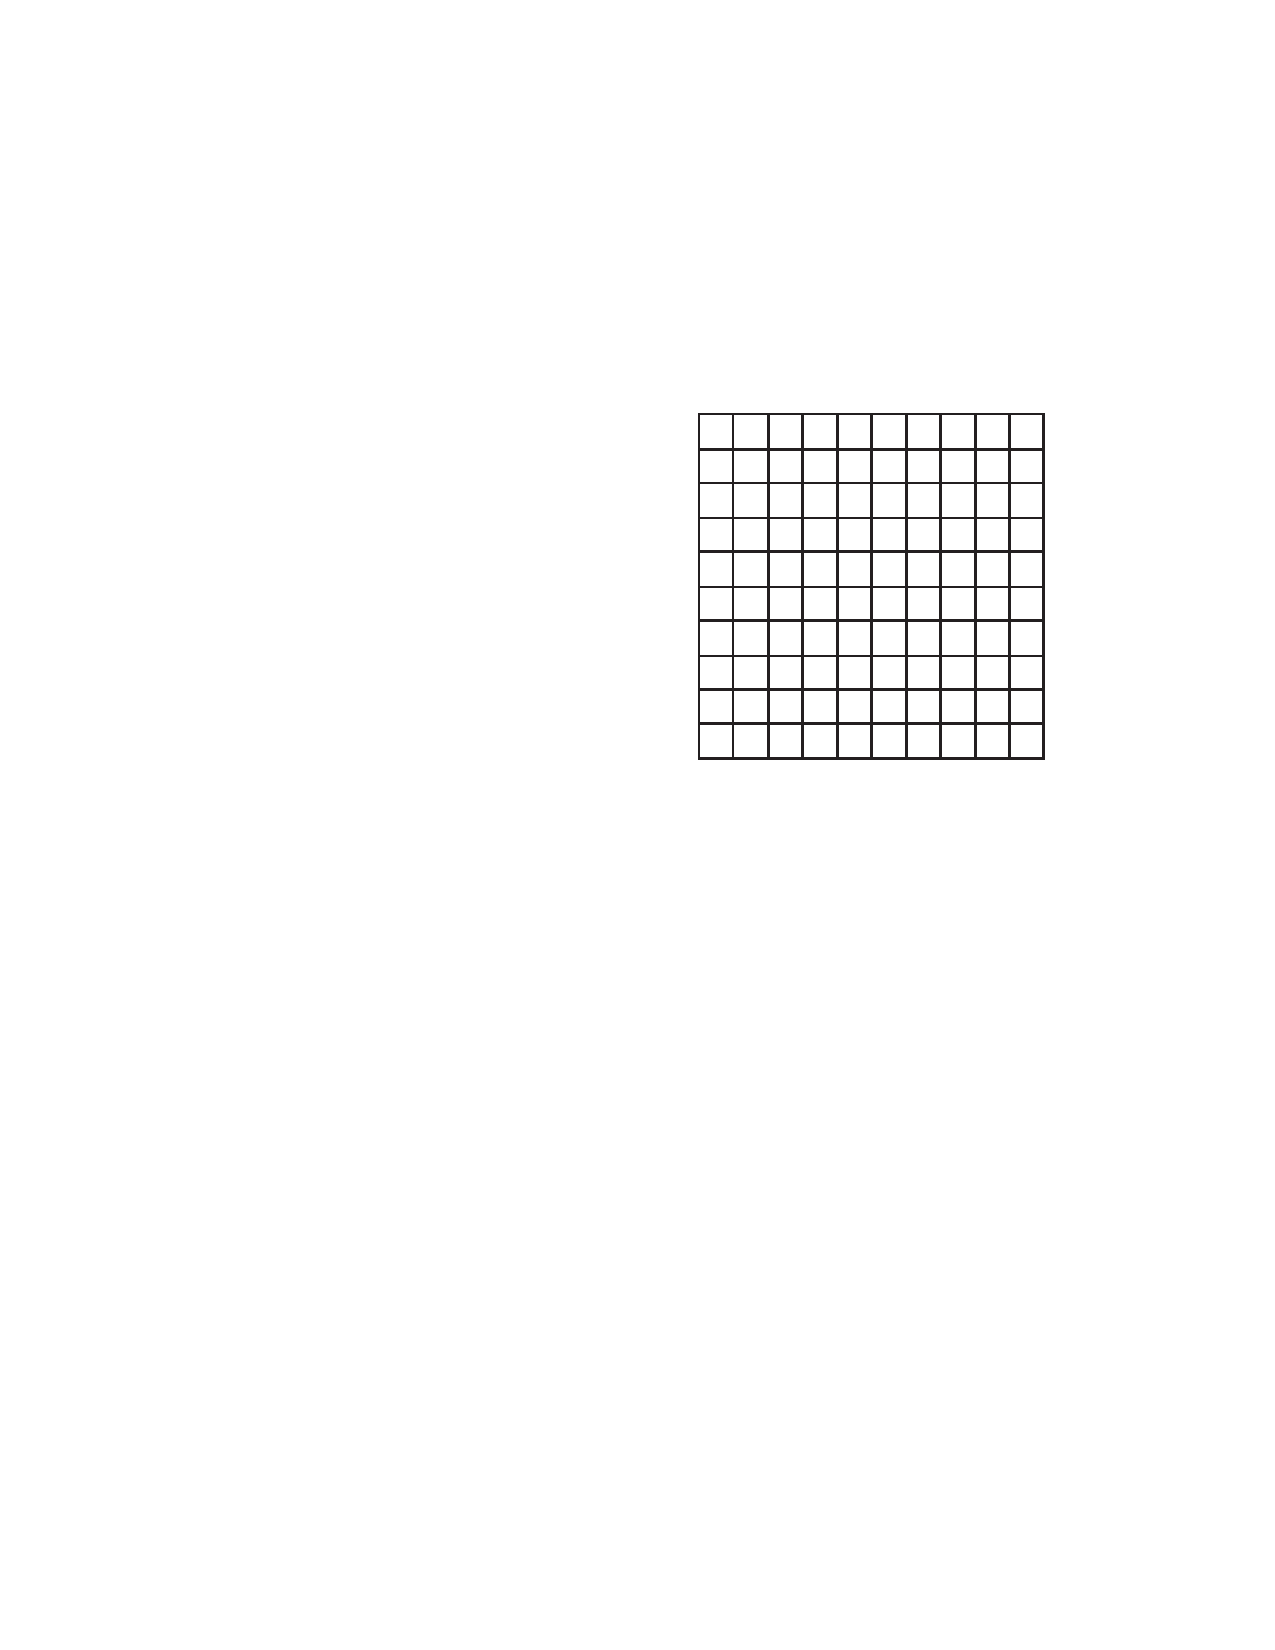
\includegraphics{../graphics/hundredthsGrid}\quad
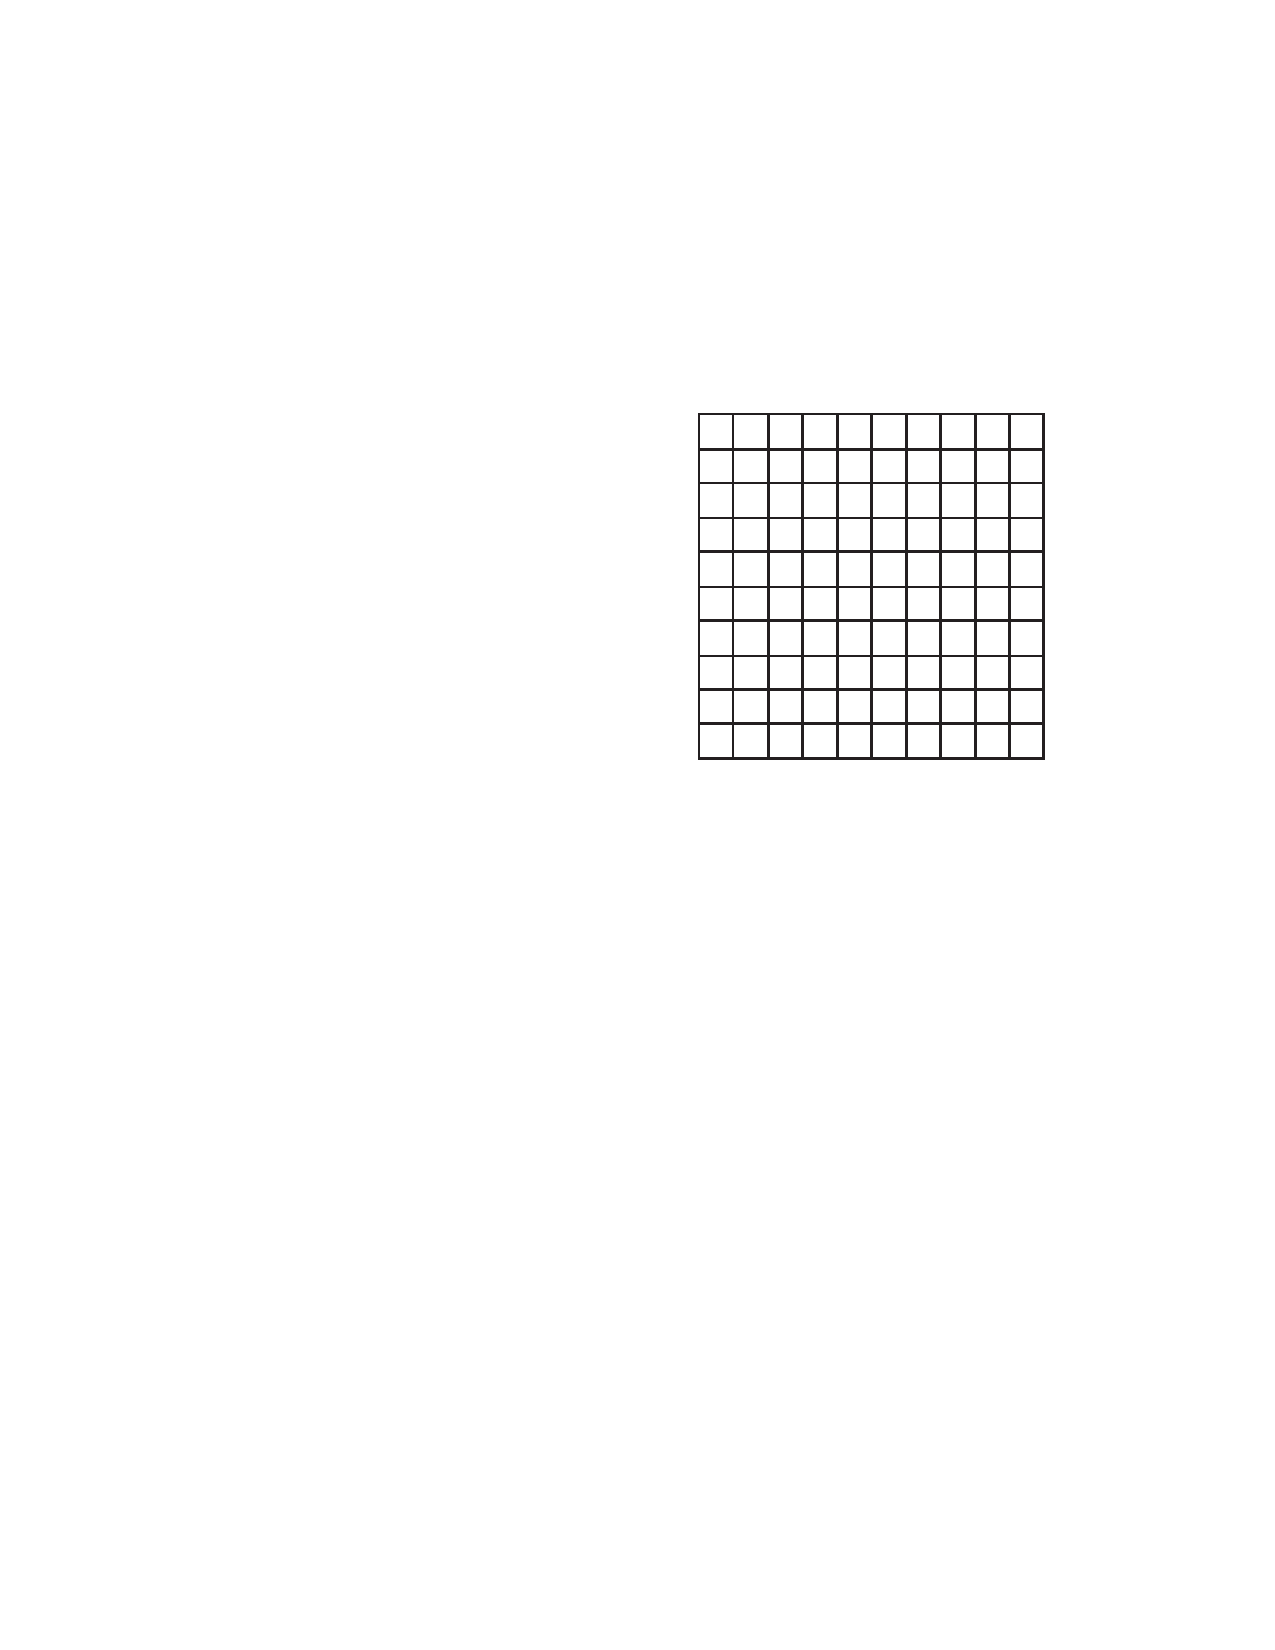
\includegraphics{../graphics/hundredthsGrid}\quad
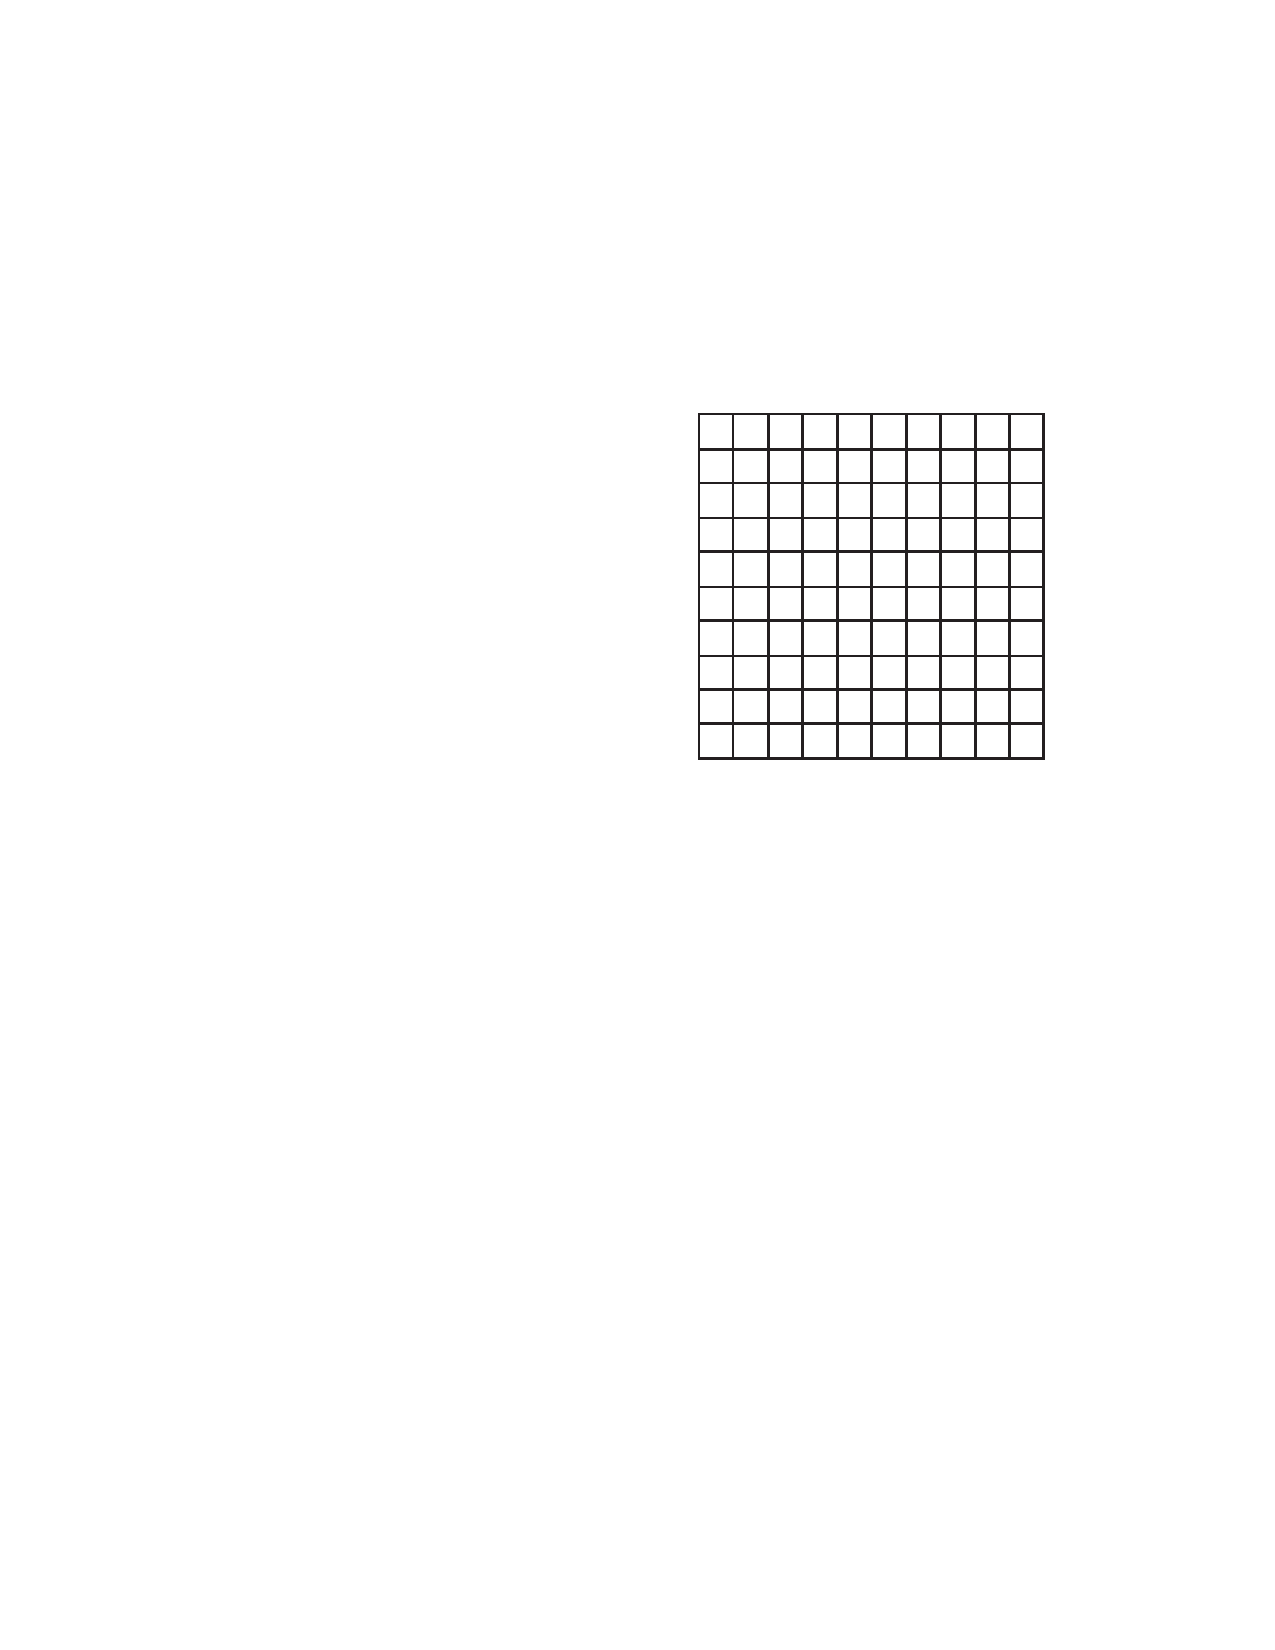
\includegraphics{../graphics/hundredthsGrid}
\end{fullwidth}

\end{prob}




\newpage
\section{Shampoo, Rinse, \dots}\label{A:Shampoo}
\index{repeating decimal}
\index{terminating decimal}

We're going to investigate the following question: If $a$ and $b$ are
integers with $b \ne 0$, what can you say about the decimal
representation of $a/b$? Let's see if we can get to the bottom of
this.

\begin{prob}\label{AR:comp} Use long division to compute $1/7$.
\end{prob}

\begin{prob}\index{Division Theorem!for integers}
State the Division Theorem for integers.
\end{prob}

\begin{prob}\label{AR:div}
Considering the solution of Problem~\ref{AR:comp}, explicitly
explain how the Division Theorem for integers appears in your work.
\end{prob}


\begin{prob} 
In each instance of the Division Theorem in Problem~\ref{AR:div}, what
is the divisor? What does this say about the remainder?
\end{prob}

\begin{prob} 
What can you say about the decimal representation of $a/b$ when $a$
and $b$ are integers with $b\ne 0$?
\end{prob}

\begin{prob} 
Assuming that the pattern holds, is the number
\[
.123456789101112131415161718192021\dots
\]
a rational number? Explain your reasoning.
\end{prob}




\begin{prob}\label{AR:exp}
Write the following fractions in decimal notation. Which have a
``terminating'' and which have a ``repeating'' decimal?
\[
\begin{array}{cccccccccc}
 \dfrac{1}{2}, &  \dfrac{1}{3}, &  \dfrac{1}{4}, &  \dfrac{1}{5}, &  \dfrac{1}{6}, & \dfrac{1}{9}, &  \dfrac{1}{10}, &  \dfrac{1}{11}, &  \dfrac{1}{12}, &  \dfrac{1}{13},  \\ \\
 \dfrac{1}{15}, & \dfrac{1}{20}, &  \dfrac{1}{24}, &  \dfrac{1}{25}, &  \dfrac{1}{28}, &  \dfrac{1}{32}, &  \dfrac{1}{35}, &  \dfrac{1}{40}, &  \dfrac{1}{42}, &  \dfrac{1}{48}.
\end{array}
\]
\end{prob}

\begin{prob}\label{AR:conj}
Can you find a pattern from your results from Problem~\ref{AR:exp}?
Use your pattern to guess whether the following fractions
``terminate'' or ``repeat.''
\[
\dfrac{1}{61}\qquad \dfrac{1}{625} \qquad \dfrac{1}{6251}
\]
\end{prob}


\begin{prob}
Can you explain why your conjecture from Problem~\ref{AR:conj} is
true?
\end{prob}


\begin{prob}\label{AR:nines} 
Compute $\frac{1}{9}$, $\frac{1}{99}$, and $\frac{1}{999}$. Can you
find a pattern? Can you explain why your pattern holds?
\end{prob}


\begin{prob}
Use your work from Problem~\ref{AR:nines} to give the fraction form of
the following decimals:
\begin{enumerate}
\item $0.\overline{357}$
\item $0.23\overline{4598}$
\item $23.\overline{459}$
\item $76.34\overline{214}$
\end{enumerate}
\end{prob}



\newpage
\section{Decimals Aren't So Nice}\label{A:DecNotNice}


\index{paradox!1=0.9@$1 = 0.999\dots$} 

We will investigate the following question: How is $0.999\dots$
related to $1$?



\begin{prob}
What symbol do you think you should use to fill in the box below?
\[
.999\dots \,\fbox{\rule[0mm]{0mm}{2mm}\hspace{2ex}}\, 1
\]
Should you use $<$, $>$, $=$ or something else entirely?
\end{prob}


\begin{prob}
What is $1 - .999\dots$?
\end{prob}

\begin{prob}
How do you write $1/3$ in decimal notation? Express
\[
\frac{1}{3} + \frac{1}{3} + \frac{1}{3}
\]
in both fraction and decimal notation.
\end{prob}

\begin{prob}
See what happens when you follow the directions below:
\begin{enumerate}
\item Set $x = .999\dots$.
\item Compute $10x$. 
\item Compute $10x-x$.
\item From the step immediately above, what does $9x$ equal?
\item From the step immediately above, what does $x$ equal?
\end{enumerate}
\end{prob}

\begin{prob}
Are there other numbers with this weird property?
\end{prob}


\newpage
\section{Ratios and Proportional Relationships}\label{A:ratioLaunch}
Here begins our work with ratios and proportional reasoning, which are the cornerstone of middle school mathematics.  Try to avoid procedural approaches, such as, ``set up a proportion and cross multiply.''  Instead, try to reason from the context and \textbf{use pictures and tables to support your reasoning}.  

As you solve these problems, note how the problems simultaneously build on understandings of fractions and pave the way for functions.  


\subsection*{Stacking Paper}
\begin{prob}
Suppose you want to know how many sheets are in a particular stack of paper, but don't want to count the pages directly. You have the following information:
\begin{itemize}
\item The given stack has height 4.50 cm.
\item A ream of 500 sheets has height 6.25 cm.
\end{itemize}
How many sheets of paper do you think are in the given stack?
\end{prob}

% From Stanley, 2014.  See more at: 
% http://blogs.ams.org/matheducation/2014/11/20/proportionality-confusion/

\begin{teachingnote}
Points to make: 
\begin{itemize}
\item To solve this problem, many people write a proportion and cross multiply, which might be fine if the only goal is the answer.  
But writing a proportion and cross multiplying misses opportunities for proportional reasoning.  
\item Draw out unit rates (80 sheets/cm and 0.0125 cm/sheet) and scale factors.  
\item Draw out quantities that are in a proportional relationship and write equations relating them.  
\item What is proportional to what?  
\end{itemize}
\end{teachingnote}

\begin{prob}
In your solution to the previous problem, what did you assume was proportional to what other quantity?  Be precise.  
\end{prob}

\subsection*{Mixing Punch}

\begin{prob}
Jenny is mixing punch and is considering two recipes:  
\begin{itemize}
\item Recipe A:  3 parts orange juice for every 5 parts ginger ale
\item Recipe B:  2 parts orange juice for every 3 parts ginger ale
\end{itemize}
\begin{enumerate}
\item Which recipe will give juice that is the most ``orangey''?  Explain your reasoning. 
\item Use a table to show various ways to make recipe B.  
\item To make 12 gallons of recipe B, how much of each will you need? 
\end{enumerate}
\end{prob}


\begin{teachingnote}
Draw out part:part versus part:whole comparisons, using quotients, common numerators, and common denominators.  In all cases, interpret the fractions and quotients.  

Use ratio tables, graphs, etc.  Note that graphs could be made relating any two of the three quantities (orange juice, ginger ale, punch).  

Draw out various unit rates:  3/5 parts orange juice for every 1 part of ginger ale... 
\end{teachingnote}

\subsection*{Racing Snails}
\begin{prob}
Mike is racing snails that move at a constant speed: 
\begin{itemize}
\item Snail A travels 3 inches in 5 minutes.  
\item Snail B travels 2 inches in 3 minutes. 
\end{itemize}
\begin{enumerate}
\item Which snail moves faster?  Explain your reasoning.
\item Use a table to show other distances and times for snail B.  
\end{enumerate}
\end{prob}


\begin{teachingnote}
These problems are very much the same as the previous problems.  But this time, the units are of different types, and they don't combine to make a new whole.  

Draw out both 2/3 in/min and 1.5 min./in as meaningful unit rates.  

Ratios are sometimes represented by fractions, but there is an important distinction:  A fraction is a single number, whereas a ratio
is often conceived as a relationship between two quantities.  
\end{teachingnote}


\newpage
\section{Poor Old Horatio}\label{A:ratios}


%  If you find that you want to write an equation, explain why the equation makes sense, and explain the steps in your solution process.  

\begin{prob}
A shade of orange is made by mixing 3 parts red paint with 5 parts
yellow paint.  Sam says we can add 4 cups of each color of paint and
maintain the same color.  Fred says we can quadruple both 3 and 5 and
get the same color.  
\begin{enumerate}
\item Who (if either or both) is correct?  Explain your reasoning.
\vspace{0.35in}

\item Use a table like the one below to show other paint mixtures that are the desired shade of orange. 
\[{\renewcommand{\arraystretch}{2}
\begin{tabular}{|c||c|c|c|c|c|c|c|c|}\hline
Red  &  3 &\rule[7mm]{12mm}{0mm} & \rule[7mm]{12mm}{0mm} & \rule[7mm]{12mm}{0mm}  & \rule[7mm]{12mm}{0mm}
 & \rule[7mm]{12mm}{0mm} & \rule[7mm]{12mm}{0mm} & \rule[7mm]{12mm}{0mm}   \\ \hline
Yellow & 5 &  &  &  & & & & \\ \hline
           &   &  &  &  & & & & \\ \hline
\end{tabular}}
\]
\end{enumerate}
\end{prob}


\begin{prob}
If we wanted to make the same orange paint but were required to use 73 cups of yellow paint, how
many cups of red paint would we need?  Explain your reasoning.  
\vspace{0.1in} 
\[{\renewcommand{\arraystretch}{2}
\begin{tabular}{|c||c|c|c|c|c|}\hline
Red  &  3 &\rule[7mm]{12mm}{0mm} &\rule[7mm]{12mm}{0mm} & \rule[7mm]{12mm}{0mm}  & \rule[7mm]{12mm}{0mm}   \\ \hline
Yellow & 5 &  &  &  & \\ \hline
           &   &   &    &  &  \\ \hline
\end{tabular}}
\]
\vspace{0.1in} 
\end{prob}


%\vspace{0.25in}

\begin{prob}
If we wanted to make the same orange paint but were required to use 56 cups of red paint, how
many cups of yellow paint would we need?  Explain your reasoning.  
\vspace{0.1in} 
\[{\renewcommand{\arraystretch}{2}
\begin{tabular}{|c||c|c|c|c|c|}\hline
Red  &  3 &\rule[7mm]{12mm}{0mm} &\rule[7mm]{12mm}{0mm} & \rule[7mm]{12mm}{0mm}  & \rule[7mm]{12mm}{0mm}   \\ \hline
Yellow & 5 &  &  &  & \\ \hline
           &   &   &    &  &  \\ \hline
\end{tabular}}
\]
\vspace{0.1in} 
\end{prob}

%\vspace{0.25in}

%\begin{prob}
%Is ``cross-multiplication''a legitimate way to solve the equations
%arising from this sort of problem---be sure to think of the weird
%units that are generated by doing so.  What good is this kooky method?
%What exactly is one doing when they ``cross-multiply'' and what type
%of problem does it solve?
%\end{prob}

\begin{prob}
Generalize your approaches to the previous problems.  
\begin{enumerate}
\item Give a general formula for computing how much red paint
is needed when $y$ cups of yellow paint is used.   
\item Give a general formula for computing how much yellow paint
 is needed when $r$ cups of red paint is used. 
\end{enumerate}
\vspace{0.1in} 
\[{\renewcommand{\arraystretch}{2}
\begin{tabular}{|c||c|c|c|c|c|}\hline
Red  &  3 &  &  &  &   \\ \hline
Yellow & 5  &\rule[7mm]{12mm}{0mm} &\rule[7mm]{12mm}{0mm} & \rule[7mm]{12mm}{0mm} & \rule[7mm]{12mm}{0mm}  \\ \hline
          &    &  &  &   &  \\ \hline
\end{tabular}}
\]
\vspace{0.1in} 
\end{prob}

\begin{prob}
Now suppose we want to make a \textbf{different shade} of orange, this time made with $\frac{3}{4}$ cup of red paint and $\frac{2}{3}$ cup of yellow paint.  How many cups of each color do you need in order to make 15 cups of the mixture?  Use the table below.  
\vspace{0.1in} 
\[{\renewcommand{\arraystretch}{2}
\begin{tabular}{|c||c|c|c|c|c|}\hline
Red  &  $\frac{3}{4}$ &  &  &  &   \\ \hline
Yellow & $\frac{2}{3}$  &\rule[7mm]{12mm}{0mm} &\rule[7mm]{12mm}{0mm} & \rule[7mm]{12mm}{0mm} & \rule[7mm]{12mm}{0mm}  \\ \hline
          &  & $17$  & $1$ & $15$   &  \\ \hline
\end{tabular}}
\]
\vspace{0.1in} 
\end{prob}

\begin{teachingnote}
Call attention to part/part vs. part/whole approaches. 
\end{teachingnote}

\begin{prob}
In proportional reasoning problems, a \emph{unit rate} describes the amount of one quantity for 1 unit of another quantity.  
\begin{enumerate}
\item What are the units for the various numbers in these problems?  
\item Identify some unit rates in this activity.  
\item In solving the above problems, it is likely that you or your classmates use strategies that made use of unit rates on the way to your solution.  Explain why this strategy is sometimes called \emph{going through one}.
\end{enumerate}
\end{prob}

\fixnote{Revise these problems drawn from Beckmann.  Use dollars/pound, or meters/second, etc.}

\begin{prob}
If $2\frac{1}{2}$ pints of jelly fills $3\frac{1}{2}$ jars, then how many jars will you need for 12 pints of jelly?  (Assume the jars are all the same size.)  If the last jar is not totally full, indicate how full it will be.  
\vspace{0.1in} 
\[{\renewcommand{\arraystretch}{2}
\begin{tabular}{|c||c|c|c|c|c|c|c|c|}\hline
Jelly  &  \rule[7mm]{12mm}{0mm} &\rule[7mm]{12mm}{0mm} & \rule[7mm]{12mm}{0mm} & \rule[7mm]{12mm}{0mm}  
 & \rule[7mm]{12mm}{0mm} & \rule[7mm]{12mm}{0mm} & \rule[7mm]{12mm}{0mm} & \rule[7mm]{12mm}{0mm}   \\ \hline
Jars &  &  &  &  & & & & \\ \hline
           &  &  &  &  & & & & \\ \hline
\end{tabular}}
\]
\vspace{0.1in} 
\end{prob}




\newpage
\section{Ratio Oddities}

In this activity we are going to investigate thinking about and adding
ratios.

\begin{prob}
There are 3 boys for every 4 girls in Mrs.\ Sanders' class.
\begin{enumerate}
\item What fraction of the class are girls? 
\item List ratios that can describe this situation. 
\item If each of the number of boys and number of girls quadruples, what is the new ratio of girls to boys?
\item Write an equation relating the number of boys in the class to the number of girls in the class.
\item If the number of boys and number of girls each increase by 6, what can you say about the new ratio of boys to girls?
\end{enumerate}
\end{prob}

\begin{prob}\label{AP:C1}
Suppose the ratio of girls to boys in Smith's class is 7:3 while the
ratio of girls to boys in Jones' class is 6:5.  
\begin{enumerate}
\item If there are 50 students in Smith's class and 55 students in Jones' class, and both
classes get together for an assembly, what is the ratio of girls to
boys? Explain your reasoning.
\item If there are 500 students in Smith's class and 55 students in Jones' class, and both
classes get together for an assembly, what is the ratio of girls to
boys? Explain your reasoning.
\item If there are 500 students in Smith's class and 55 students in Jones' class, and both
classes get together for an assembly, what is the ratio of girls to
boys? Explain your reasoning.
\item Now suppose you don't know how many student are in Smith's class and there are 55 students in Jones' class. What is the best answer you can give for the ratio of girls to boys at the assembly. 
\end{enumerate}
\end{prob}


\begin{prob}
Suppose you are teaching a class, and a student writes
\[
\frac{1}{4} + \frac{3}{5} = \frac{4}{9}
\]
\begin{enumerate}
\item How would you respond to this? 
\item This student is most contrary, and presents you with the following problem:
\begin{quote}
Suppose you have two cars, a 4 seater and a 5 seater. If the first car
is $1/4$ full and the second car is $3/5$ full, how full are they
together?
\end{quote}
The student then proceeds to answer their question with ``The answer
is $4/9$.'' How do you address this?
\end{enumerate}
\begin{teachingnote}
You might want to ask what happens if the first car is $1/4$ full and $6/10$ full.
\end{teachingnote}
\end{prob}



\begin{prob}\label{AP:C2}
Again, suppose the ratio of girls to boys in Smith's class is 7:3
while the ratio of girls to boys in Jones' class is 6:5.  If there are
40 students in Smith's class and 55 students in Jones' class, and both
classes get together for an assembly, what is the ratio of girls to
boys at the assembly? Explain your reasoning.
\end{prob}


\begin{prob} 
Let's use $\oplus$ for this new form of ``addition.'' So
\[
\frac{a}{b} \oplus \frac{c}{d} = \frac{a+c}{b+d}.
\]
I claim that in Problem~\ref{AP:C1} we could solve using
\[
\frac{a}{b} \oplus \frac{c}{d} = \frac{a+c}{b+d}.
\]
However, in Problem~\ref{AP:C2} we could not. What is going on here?
\end{prob}



\begin{prob} 
Let's think a bit more about $\oplus$. If you were going to plot
$\frac{a}{b}$ and $\frac{c}{d}$ on a number line, where is
$\frac{a}{b} \oplus \frac{c}{d}$? Is this always the case, or does it
depend on the values of $a$, $b$, $c$, and $d$? You should give an
explanation based on context, and an explanation based on algebra.
\end{prob}

\begin{teachingnote}
Here you will probably not only want to have the students realize that
$\frac{a}{b} \oplus \frac{c}{d}$ is between both $\frac{a}{b}$ and
$\frac{c}{d}$, but that the location varies by which denominator is
largest.
\end{teachingnote}





%\newpage
\section{Problem Solved!}\label{A:ProblemSolved}

Here's an old puzzler:


\begin{prob}
A man is riding a camel across a desert when he encounters a novel
sight. Three young men are fiercely arguing surrounded by 17
camels. Dismounting, the stranger was told that their father had died,
leaving (as their only real inheritance) these 17 camels. Now, the
eldest son was to receive half of the camels, the second son one-third
of the camels, the youngest son one-ninth of the camels. How could
they divide the 17 camels amongst themselves?  Explain your
reasoning.
\end{prob}

Uncharacteristically, I will solve this problem for you:

\begin{proof}[Solution] 
The man should generously add his camel to the $17$ being argued
over. Now there are $18$ camels to divide amongst the three
brothers. With this being the case:
\begin{itemize}
\item The eldest son receives $9$ camels.
\item The middle son receives $6$ camels.
\item The youngest son receives $2$ camels.
\end{itemize}
Ah! Since $9+6+2 = 17$, there is one left over, the man's original
camel---he can now have it back.
\end{proof}

\begin{prob}
What do you think of this solution?
\end{prob}

\begin{prob}
Describe your thought process when addressing the above
problem.
\end{prob}


\newpage
\section{The Triathlete}\label{A:Triathlete}

\begin{prob} 
On Friday afternoon, just as Laine got off the bus, she realized that she had left her bicycle at school.  In order to have her bicycle at home for the weekend, she decided to run to school and then ride her bike back home.  If she averaged 6 mph running and 12 mph on her bike, what was her average speed for the round trip?  Explain your reasoning. 
\end{prob}

\begin{teachingnote}
A key idea here is that the average speed is independent of the distance.  Here are several ways that students can solve it: 
\begin{itemize}
\item Pick a distance, say 12 miles.  Then running to school will take 2 hours, and biking back home will take 1 hour.  That's a total of 24 miles in 3 hours, or an average of 8 mph.  
\item Let the distance be $d$.  Then running to school will take $\frac{d}{6}$ hours, and biking back home will take $\frac{d}{12}$ hours.  The total distance is $2d$.  So the average rate is 

$$\frac{2d}{\frac{d}{6}+\frac{d}{12}}=\frac{2}{\frac{1}{6}+\frac{1}{12}}=\frac{2}{\frac{3}{12}}=\frac{2}{\frac{1}{4}}=8 \text{ mph}$$
Notice that the $d$ factors out of both the numerator and the denominator (and hence cancels), which shows that the average speed is independent of the distance.  

Notice also that this calculation can be expressed as a different kind of average:  $$\frac{\frac{1}{6}+\frac{1}{12}}{2}=\frac{1}{8}$$
This average is called the \emph{harmonic mean}.  Specifically, 8 is the harmonic mean of 6 and 12 because it is the reciprocal of the average of their reciprocals.  (Math 1165 students do not need to know this language.)
\item Sometimes is helpful to think of speed as ``time per distance,'' which is the reciprocal of ``distance per time.''  In this problem, we can reason that Lanie runs a ``ten-minute mile" as follows:  Her speed of 6 mph would be $\frac{1}{6}$ hour/mile, which is the same as 10 min/mile.  Similarly, she bikes at 5 min/mile.  With this insight, we can cut the distance between home and school into 1-mile pieces and reason that she will take 10 minutes to run each mile and 5 minutes to bike the same mile on the way home.  That would be 15 minutes for both directions (2 miles), for an average speed of 7.5 min/mile, which is the same as 8 mph.  
\item Another way of thinking about these kinds of problems is as weighted averages.  For example, because the distances are the same, Laine will spend twice as much time running (i.e., at half the speed) as she spends on her bike.  Thus, we can weight the 6 mph running speed twice and the 12 mph biking speed just once, as follows:  
$$\textrm{Average speed }= \frac{2\cdot6 + 12}{3} = 8.$$
Notice we divide by 3 because that is the sum of the weights.  The same reasoning can work even when the numbers are more challenging.  
\end{itemize}
\end{teachingnote}

\begin{prob}
On Saturday, Laine completed a workout in which she split the time evenly between running and cycling.  If she again averaged 6 mph running and 12 mph on her bike, what was her average speed for the workout?  Explain your reasoning. 
\end{prob}

\begin{teachingnote}
Here the naive calculations works:  The average speed is the average of the two speeds, so the answer is $\frac{6+12}{2}=9$ mph.  But we should be clear why this works.  Here are two approaches: 
\begin{itemize}
\item Pick a time, say 1 hour, to spend on each activity.  Lanie will run 6 miles in 1 hour and will bike 12 miles in 1 hour.  That will be 18 miles in 2 hours, or an average of 9 mph.  This will work, of course, for every hour of activity, which suggests that the result is independent of time.  
\item Algebra:  Let the $t$ represent the time spent on each activity.  The distance running will be $6t$, the distance biking will be $12t$, and the total time will be $2t$.  So the average speed will be $$\frac{6t+12t}{2t}=\frac{18t}{2t}=9 \text{ mph.}$$  
Notice the common factor of $t$ cancels, which shows that the average speed is independent of the time.  
\end{itemize}
\end{teachingnote}

\begin{prob}
Why was her average speed on Saturday different from her average speed on Friday?  Can you reason, without computation, which average speed should be faster?  
\end{prob}

\begin{teachingnote}
One approach:  When the times are the same, the average will be midway between the two speeds.  When the distances are the same, in contrast, she will spend more time traveling at the slower speed than at the faster speed, so the average will be closer to the slower speed, which implies that the same-distance average is slower than the same-time average.  
\end{teachingnote}

\begin{prob} On Sunday, Laine's workout included swimming.  Assuming that she can swim at an average speed of 2 mph, describe two running-cycling-swimming workouts, one similar to Friday's scenario (same distance) and a second similar to Saturday's (same time).  Compute the average speed for each and explain your reasoning.  
\end{prob}

\begin{teachingnote}
Same distance (a la Friday):  

$$\text{Average speed } = \frac{3d}{\frac{d}{2}+\frac{d}{6}+\frac{d}{12}}=\frac{3}{\frac{1}{2}+\frac{1}{6}+\frac{1}{12}}=\frac{3}{\frac{9}{12}}=\frac{3}{\frac{3}{4}}=4  \text{ mph.}$$

Same time (a la Saturday):  $$\text{Average speed } = \frac{2t+6t+12t}{3t}=\frac{20t}{3t}=6\frac{1}{3} \text{ mph.}$$
\end{teachingnote}

\begin{prob}
Which of the workout scenarios (same distance or same time) most closely resembles an actual triathlon?  Why do you think that is the case?
\end{prob}

\begin{teachingnote}
In actual triathlons, the running distances are much shorter than the biking distances, and the swimming distances are much shorter still.  It would not be reasonable to swim any reasonable biking distance.  So the ``same time'' scenario is closer.  But in reality, the swimming times are quite a bit shorter than the running and biking times.  
\end{teachingnote}

\begin{prob}
After two months of intense training, Laine is able to average $s$ mph swimming, $r$ mph running, and $c$ mph cycling.  Again describe two running-cycling-swimming workouts, one similar to each of the two original scenarios, and compute her average speeds.     
\end{prob}

\begin{teachingnote}
Same distance (a la Friday):  

$$\text{Average speed } = \frac{3d}{\frac{d}{s}+\frac{d}{r}+\frac{d}{c}}=\frac{3}{\frac{1}{s}+\frac{1}{r}+\frac{1}{c}}$$

Same time (a la Saturday):  $$\text{Average speed } = \frac{st+rt+ct}{3t}=\frac{(s+r+c)t}{3t}=\frac{s+r+c}{3}$$
\end{teachingnote}


\newpage
\section{The Dreaded Story Problem}\label{A:dreadedStoryProblem}

Let's try our hand at a problem involving ratios.

\begin{teachingnote}
This problem is challenging. Students must try out actually
numbers and do experiments. There are many false ``solutions'' that can be obtained.
\end{teachingnote}


\begin{prob}
On orders from his doctor, every day, Marathon Marty must run from his
house to a statue of Millard Fillmore and run back home along the same
path.  So Marty doesn't lollygag, the doctor orders him to average 8
miles per hour for the round trip or endure painful electrical shock
therapy to his big toes.  Today, Marty ran into Gabby Gilly on his way
to the statue and averaged only 6 miles per hour for the trip out to
the statue.
\begin{enumerate}
\item Name some quantities that might be associated with this problem.
Which of the quantities are constant and which can change? Which
quantities affect Marty's average rate for the round trip and what are
those effects?

\item What must Marty do to ensure he's obeyed his doctor's orders? 
Once your model is set up, solve the problem in as many ways that you
can (guess and check, algebraically, graphically, with tables, pure
reasoning, etc.).

\item Assume the doctor orders him to average 8.346 miles per hour for the round trip.
Today, Marty ran into Gabby Gilly on his way to the statue and
averaged only 6.597 miles per hour for the trip out to the statue.
What must Marty do to ensure he's obeyed his doctor's orders?
\item Now assume the doctor orders him to average 6 miles per hour for the round trip.
Being fired up, Marty ignores Gabby Gilly and averages 8 miles per
hour on the way out.  What must Marty do to ensure he's obeyed his
doctor's orders?
\item The doctor now goes back and orders Marty to average 8 miles per hour for the round trip again.
This time, Gabby Gilly tackles Marty and starts yakking at him so much
that Marty only averages 4 miles per hour on the way out.  What must
Marty do to ensure he's obeyed his doctor's orders?
\item Now the doctor orders him to average n miles per hour for the round trip.
Assuming that Marty, for whatever reason, averages m miles per hour on
the trip out to the statue. What must Marty do to ensure he's obeyed
his doctor's orders?
\end{enumerate}
\end{prob}

\begin{prob}
What changes can you make to this problem to make it different?
Easier? Harder?
\end{prob}


\newpage
\section{I Walk the Line}\label{A:walk}
\fixnote{As best as you can, solve these problems initially without using letters.}  

\begin{prob}
Slimy Sam is on the lam from the law.  Being not-too-smart, he drives
the clunker of a car he stole east on I-70 across Ohio.  Because the
car can only go a maximum of 52 miles per hour, he floors it all the
way from where he stole the car (just now at the Rest Area 5 miles
west of the Indiana line) and goes as far as he can before running out
of gas 3.78 hours from now.

\begin{enumerate}
\item At what mile marker will he be 3 hours after stealing the car?
\item At what mile marker will he be when he runs out of gas and is
  arrested?
\item At what mile marker will he be $x$ hours after
  stealing the car?
\item At what time will he be at mile marker 99 (east of Indiana)?
\item At what time will he be at mile marker 71.84?
\item At what time will he be at mile marker $y$?
\item Do parts (c) and (f) supposing that the car
  goes $m$ miles per hour and Sam started $b$ miles east of the
  Ohio-Indiana border.
\item What ``form'' of an equation for a line does this problem
  motivate?
\end{enumerate}
\end{prob}

\begin{prob}
Free-Lance Freddy works for varying hourly rates, depending on the
job.  He also carries some spare cash for lunch.  To make his
customers sweat, Freddy keeps a meter on his belt telling how much
money they currently owe (with his lunch money added in).
\begin{enumerate}
\item On Monday, 3 hours into his work as a gourmet burger flipper,
  Freddy's meter reads $\$42$. 7 hours into his work, his meter reads
  $\$86$.  If he works for 12 hours, how much money will he have?  When
  will he have $\$196$? Solve this problem \textbf{without} finding his
  lunch money.
\item On Tuesday, Freddy is CEO of the of \textit{We Say So} Company.
  After 2.53 hours of work, his meter reads $\$863.15$ and after 5.71
  hours of work, his meter reads $\$$1349.78.  If he works for 10.34
  hours, how much money will he have?  How much time will he be in
  office to have $\$$1759.21?
\item On Wednesday, Freddy is starting goalie for the \textit{Columbus
  Blue Jackets}. After $x_1$ hours of work, his meter reads $y_1$
  dollars and after $x_2$ hours of work, his meter reads $y_2$
  dollars. Without finding his amount of lunch money, if he works for
  $x$ hours, how much money will he have?  How much time will he be in
  front of the net to have $y$ dollars?
\item What ``form'' of an equation for a line does this problem
  motivate?
\end{enumerate}
\end{prob}

\begin{prob} 
Counterfeit Cathy sells two kinds of fake cereal: Square Cheerios for
$\$$4 per pound and Sugarless Sugar Pops for $\$$5 per pound.

\begin{enumerate}
\item If Cathy's goal for today is to sell $\$$1000 of cereal, how
  much of each kind could she sell? Give five possible answers.
\item Plot your answers.  What does the slope represent in this
  situation? What do the points where your curve intercepts the axes
  represent?
\item If she sells Square Cheerios for $a$ dollars per pound and
  Sugarless Sugar Pops for $b$ dollars per pound and she wants to sell
  $c$ dollars of cereal, write an equation that relates the amount of
  Sugar Pops Cathy sells to the amount of Cheerios she sells.  What
  ``form'' of the equation of a line does this problem motivate?
\item Write a function in the form 
\[
\text{pounds Sugar Pops Sold} = f(\text{pounds of Cheerios sold}).
\]
\end{enumerate}
\end{prob}


\begin{prob}
Given points $p= (3,7)$ and $q = (4,9)$, find the formula for the line
that connects these points.
\end{prob}


\begin{prob}
In each of the situations above, write an equation relating the two
variables (hours and position, hours and current financial status,
pounds of Square Cheerios and pounds of Sugarless Sugar Pops) and
answer the following questions:
\begin{enumerate}
\item How did (or could) the equations help you solve the problems
  above? What about a table or a graph?
 \item Organize the information in each problem into a table and then
 into a graph.  What patterns do you see, if any?
  \item  What do the different features of your graph represent for each situation?
 \end{enumerate}
\end{prob}


\newpage
\section{Constant Amount Changes}\label{A:ConstantAmount}

In this section, we explore sequences and functions and the fact that sequences are functions. 

Sometimes you compute the output value of a function from a previous output value.  This is called a \emph{recursive} representation of the function.  Other times, you compute the output value directly from the input value.  This is called a \emph{closed form} representation of the function.  Both approaches are important, as they provide different insights.  

\begin{prob}
We can use function notation for sequences, with $f(n)$ representing the $n^\mathrm{th}$ term of a sequence.  Here is an example of a sequence specified recursively:  
$$f(0) = 1\text{, }f(1) = 1,\text{ and }f(n) = f(n-1)+f(n-2)\text{ for }n \ge 2.$$
\begin{enumerate}
\item Find $f(6)$ and explain your reasoning.  
\item Why was it important to give the values $f(0) = 1$ and $f(1) = 1$?  
\end{enumerate}
\end{prob}

\begin{prob}%\label{P:gtg1}
Gertrude the Gumchewer has an addiction to Xtra Sugarloaded Gum, and it's getting worse.  At the beginning of her habit, on day 0, she chews 3 pieces and then, each day afterward, she chews 8 more pieces than she chewed the day before.
\begin{enumerate}
\item Gertrude's friend Wanda notices that Gertrude chewed 35 pieces on day 4.  Wanda claims that, because Gertrude is increasing the number of pieces she chews at a constant rate, we can just use proportions with the given piece of information to find out how many pieces Gertrude chewed on any other day.  Is Wanda correct or not?  Explain. 
\item Make a table of how many pieces of gum Gertrude chewed on each of the first 10 days of her addiction.  
\item Think of what a $4^\mathrm{th}$ grader would do to predict the next day's number of pieces given the previous day's number of pieces.  Use the variables $Next$ and $Now$ to write an equation that describes the thinking.
\item Write a recursive specification for a function $g(n)$ that gives the number of pieces of gum Gertrude chewed on the $n^\mathrm{th}$ day.  
\item How many pieces of gum Gertrude did chew on the $793^\mathrm{rd}$ day of her habit?  Explain your reasoning.  
\item How would the $4^\mathrm{th}$ grader answer the previous question?  How does this differ from how you solved it?
\item Write a closed formula for computing $g(n)$ directly from $n$.  
\item Make a graph of your data about Gertrude's gum chewing.  Which variable do you plot on the horizontal axis?  Explain.  
\item Does it make sense to connect the dots on your graph?  Explain.  
\item  Locate the values $g(6)$ and $g(5)$ in your table from above, compute  $g(6) - g(5)$, and interpret your result.  How might you have known the answer without doing any calculation?  
\end{enumerate}
\end{prob}

\begin{prob}
Slimy Sam steals a car from a rest area 3 miles east of the Indiana-Ohio state line and starts heading east along the side of I-70.  Because the car is a real clunker, it can only go 8 miles per hour.  
\begin{enumerate}
\item Assuming the police are laughing too hard to arrest Sam, describe Sam's position on I-70 (via mile markers) $t$ hours after stealing the car.  
\item Make a graph of your data about Sam's travel.  Which variable do you plot on the horizontal axis?  Explain.  
\item Does it make sense to connect the dots on your graph?  Explain your reasoning.  
\item Write a recursive specification for a function $s(t)$ that gives Sam's position on I-70 at hour $t$.  
\item Write closed formula for $s(t)$.  
\item How is this problem the same and how is it different from the Gertrude problem?  
\item Dumb Question:  At any specific time, how many positions could Sam be in? 
\end{enumerate}
\end{prob}


\newpage
\section{Constant Percentage (Ratio) Changes}\label{A:ConstantRatio}
\fixnote{Give them a table and a graph.  Or put them in the margin.}

\begin{prob}
Billy is a bouncing ball.  He is dropped from a height of 13 feet and each bounce goes up 92\% of the bounce before it.  Assume that the first time Billy hits the ground is bounce 1.  

\begin{enumerate}
\item Make a table of how high Billy bounced after each of the first 10 times he hit the ground.  Be sure to indicate the arithmetic process you go through for each bounce (i.e., not just the final height).  Find a pattern that will predict an answer.  

\item Think of what a $7^\mathrm{th}$ grader would do to predict the next bounce's height given the previous bounce's height.  How would the $7^\mathrm{th}$ grader answer the previous question?  How does this differ from how you solved it?

\item Make a graph of your data about Billy.  Which variable do you plot on the horizontal axis?  Explain.  

\item Does it make sense to connect the dots on your graph?  Explain your reasoning.  

\item How high will Billy bounce after the 38th bounce?  How high will Billy bounce after the $n^\mathrm{th}$ bounce?  Explain your reasoning. 

\item  Use function notation, $f(n)$, and a recursive formula to specify the height of Billy's bounces, including the initial condition and general term.   

\item Use function notation, $f(n)$, and an explicit formula to specify the height of Billy's bounces.  Indicate the domain of the function.    

\item Using your table from above, compute the differences between the heights on successive bounces (e.g.,  $f(1) - f(0)$, $f(2) - f(1)$, etc.).  What do you notice?  Why does this happen?

\item Compare and contrast the explicit and recursive representations from Billy and from Gertrude.  How do the role(s) of the operations and initial values differ, remain the same, or relate?
\end{enumerate}
\end{prob}

\begin{prob}
Supppose 13 mg of a drug is administered to a patient once, and the amount of the drug in the patient's body decreases by 8\% each hour.  
\begin{enumerate}
\item Describe the amount of the drug in the patient's body $t$ hours after it was administered.  

\item Make a graph of your data about the amount of drug in the body over time.  Which variable do you plot on the horizontal axis?  Explain.  

\item Does it make sense to connect the dots on your graph?  Explain your reasoning.  

\item Use function notation, $g(t)$, and an explicit formula to specify the the amount of drug remaining in the body after $t$ hours.  Indicate the domain of the function. 

\item How is this problem fundamentally different from the Billy problem?  What is the same and different about the functions $f$ and $g$?  

\item Dumb Question:  At any one time, how many different amounts of the drug are possible in the patient's body?
\end{enumerate}
\end{prob}


%\newpage
\section{Rules of Exponents}\label{A:ExponentRules}

\fixnote{Fold in new activity here.}  

\begin{prob}
Attendance at a picnic consistently grows by 21\% each year.  The attendance this year was 5678.    
\begin{enumerate}
\item Write both a recursive and explicit representation of the relationship between the number of years and the attendance.  Use 2013 as ``year 0.''

\item Using only the attendance for 2018, how would you find the attendance for 2024 by doing only one multiplication?  What rule from school mathematics supports your solution process?
      
\item Using only the explicit form of the relationship, predict what the attendance was in 2010.  Now find the same information by only using the attendance in 2018 and one division. What rule from school mathematics supports your solution process?
     
\item What was the attendance in 2013?  What rule from school mathematics supports your solution process?
\end{enumerate}
\end{prob}
\begin{prob}
What is wrong with the following statement:  ``$5^7$ is 5 multiplied by itself 7 times.''  If the statement were true, what would $5^1$ be?  What would $5^0$ be?
\end{prob}
\begin{prob}
Why is $x^3$ not the same function as $3^x$?  We often think of multiplication as ``repeated addition,'' and we find that adding $a$ copies of $b$ gives the same result as adding $b$ copies of $a$.  Does this idea work for thinking of exponentiation as ``repeated multiplication''?  Explain.  
\end{prob}

\begin{prob}
Joe Schmo saved the King's daughter from a vicious dragon.  For such gallantry, the King offers Joe the choice of two payment plans: 
\begin{itemize}
\item Plan \#1:  \$1 today, and on subsequent days Joe will have an amount that is the cube of the day number (so, for example, on day 2, Joe  will have \$8). 
\item Plan \#2:  \$1 today, and on subsequent days Joe will have 2\% more than the previous day (for example, on Day \#2, he'll have \$1.02).  
\end{itemize}
Note that Joe must deposit the previous day's money in order to get today's money.  Assuming he wants the plan that yields the most money, which plan should he pick?  Explain your reasoning.  
\end{prob}
  Replaced by Meanings of Exponents

\newpage
\section{Meanings of Exponents} 

Students in grades 3-7 can use their understanding of counting number arithmetic to build understandings of the arithmetic of negative integers and rational numbers.  Here are the key ideas: 
\begin{quote}
\begin{itemize}
\item The properties of operations (commutative, associative, and distributive properties) are established for counting numbers based on meanings of operations. 
\item As we extend arithmetic to negative integers and rational numbers, we want the properties of operations to continue to hold.  
\end{itemize}
\end{quote}

This activity follows an analogous process for exponents: Students use their understanding of counting number exponents to build an understanding of negative integer and rational exponents.  Here are the key ideas: 
\begin{quote}
\begin{itemize}
\item The rules of exponents are established for counting number exponents based on the meaning of an exponent.  
\item As we extend to negative and rational exponents, we want the rules of exponents to continue to hold.  
\end{itemize}
\end{quote}

\begin{prob}
Students sometimes say that $a^n$ means ``$a$ multiplied by itself $n$ times.''  But for counting number exponents, this is not correct.  For example, how many multiplications are there in $3^5$?  Write a better definition for $a^n$, where $n$ is a counting number.  
\end{prob}

\begin{prob}
Why is $x^3$ not the same function as $3^x$?  We often think of multiplication as ``repeated addition,'' and we find that adding $a$ copies of $b$ gives the same result as adding $b$ copies of $a$.  Does this idea work for thinking of exponentiation as ``repeated multiplication''?  Explain.  
\end{prob}

\begin{prob}
If you do not know (or do not remember) the rules for exponents, you can still use your definition of $a^n$ to figure out other ways of writing expressions with exponents.  Use \textbf{specific values} for letters in expressions of the form $a^na^m$, 
$a^n/a^m$, $(a^n)^m$, and $(ab)^n$ for counting-number exponents, to explain what the rules must be.  Choose specific values that help you explain generally.  
\end{prob}

\begin{prob}
\textbf{Patterns.}  One way to reason about the meanings of zero and negative exponents is to use patterns.  As you complete the following table, \textbf{imagine that you know nothing about zero and negative exponents.}  Instead, use the patterns in the values for positive exponents to reason about what the values should be for zero and negative exponents.  Then reason generally about the meaning of $a^0$ and $a^{-n}$, where $n$ is a counting number and $a$ is a real number.  Are there any values of $a$ for which your reasoning is not valid?  Explain.  
\end{prob}

\begin{minipage}{0.3\textwidth}
\begin{align*}
2^3 &=  \\
2^2 & = \\
2^1 &= \\
2^0 &= \\
2^{-1} &= \\
2^{-2} &= \\
2^{-3} &= \\
\end{align*}
\end{minipage}
\begin{minipage}{0.3\textwidth}
\begin{align*}
3^3 &=  \\
3^2 & = \\
3^1 &= \\
3^0 &= \\
3^{-1} &= \\
3^{-2} &= \\
3^{-3} &= \\
\end{align*}
\end{minipage}
\begin{minipage}{0.3\textwidth}
\begin{align*}
(-2)^3 &=  \\
(-2)^2 & = \\
(-2)^1 &= \\
(-2)^0 &= \\
(-2)^{-1} &= \\
(-2)^{-2} &= \\
(-2)^{-3} &= \\
\end{align*}
\end{minipage}
\begin{minipage}{0.3\textwidth}
\begin{align*}
\left(\frac{1}{2}\right)^3 &=  \\
\left(\frac{1}{2}\right)^2 & = \\
\left(\frac{1}{2}\right)^1 &= \\
\left(\frac{1}{2}\right)^0 &= \\
\left(\frac{1}{2}\right)^{-1} &= \\
\left(\frac{1}{2}\right)^{-2} &= \\
\left(\frac{1}{2}\right)^{-3} &= \\
\end{align*}
\end{minipage}


\begin{prob}
\textbf{Extending the rules.}  A careful way to approach zero and negative integer exponents is to use the rules of exponents (which you established above for counting-number exponents) to determine what 0 and negative integer exponents must mean if the exponent rules continue to hold in this extended domain.
\begin{enumerate}
\item Use the exponent rules to provide two explanations for a sensible definition of $a^0$, being clear about why your definition makes sense.  Note any restrictions on $a$.  
\item Use the exponent rules to provide two explanations for a sensible definition of $a^{-n}$, where $n$ is a counting number.  Again, note any restrictions on $a$.
\end{enumerate}
\end{prob}

\begin{prob}
While trying to decide what $3^{\frac{2}{5}}$ should mean, Katie wondered about the expression $\left(3^{\frac{2}{5}}\right)^5$.  What should Katie's expression be equal to?  Explain, using rules of exponents.  Then use Katie's idea to determine a value for $3^{\frac{2}{5}}$.  
\end{prob}





%\newpage
\section{Something Doesn't Add Up\dots}\label{A:doesntAddUp}

\fixnote{Move these to problems.}

\begin{prob}\label{P:sdau2}
Sum all the counting numbers starting with $551$ and ending at
$5051$. Use the rows of numbers below to help you.
\[
\begin{array}{c@{ + }c@{ + }c@{ + }c@{ + }c@{ + }c@{ + }c@{ + }c@{ + }c@{ + }c@{ + }c@{ + }c@{ + }c}
551 & 552 & 553 & 554 & 555 & 556 & \cdots & 5046 & 5047 & 5048 & 5049 & 5050 & 5051 \\
5051 & 5050 & 5049 & 5048 & 5047 & 5046 & \cdots & 556 & 555 & 554 & 553 & 552 & 551 
\end{array}
\]
Explain your reasoning---be sure to clearly explain what happens in
the ``dots.''  
\end{prob}


\begin{prob}\label{P:sdau1}
How many unshaded circles are in the diagram below? 
\[
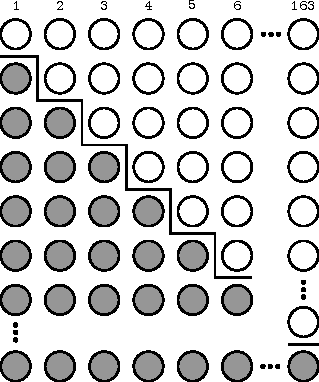
\includegraphics{../graphics/sum1.pdf}
\]
Explain your reasoning---be sure to clearly explain what happens in
the ``dots.'' Compare this with question \ref{P:sdau2}.
\end{prob}



\begin{prob}
Sum the numbers:  
\[
106 + 112 + 118 + \dots + 514
\]
Compare this with questions \ref{P:sdau1} and \ref{P:sdau2} above.
\end{prob}

\begin{prob}
Sum the numbers:
\[
2.2 + 2.9 + 3.6 + 4.3 + \dots + 81.3
\]
\end{prob}


  Replaced by arithmetic series

%\newpage
\section{The World Series}\label{A:WorldSeries}

\begin{prob}
Recall the story of Gertrude the Gumchewer, who has an addiction to Xtra Sugarloaded Gum.  Each day, she goes to her always stocked storage vault and grabs gum to chew.  At the beginning of her habit, she chewed three pieces and then, each day, she chews eight more pieces than she chewed the day before to satisfy her ever-increasing cravings. We want to find out how many pieces of gum did Gertrude chew over the course of the first 973 days of her habit?

\end{prob}

\begin{prob}\label{P:gtg2}
Assume now that Gertrude, at the beginning of her habit, chewed $m$
pieces of gum and then, each day, she chews $n$ more pieces than she
chewed the day before to satisfy her ever-increasing cravings.  How many pieces will she chew over the course of the first $k$
  days of her habit? Explain your formula and how you know it will work for any $m$, $n$ and $k$.  
\end{prob}

\begin{prob}
Use the method you developed in questions \ref{P:gtg1} and
\ref{P:gtg2} to find the sum:
\[
19 + 26 + 33 + \dots + 1720
\]
Give a story problem that is represented by this sum.
\end{prob}

\begin{prob}
Now remember the story of Billy the bouncing ball.  He is dropped from a height of 13 feet and each bounce goes up 92\% of the bounce before it.  Assume that the first time Billy hits the ground is bounce \#1.  How far did Billy travel over the course of 38 bounces (up to when he hits the ground on his 38th bounce)?  
\end{prob}

\begin{prob}
Assume now that Billy the Bouncing Ball is dropped from a height of
$h$ feet. After each bounce, Billy goes up a distance equal to $r$
times the distance of the previous bounce. (For example, $r=.92$ above.)
\begin{enumerate}
\item How high will Billy go after the $k$th bounce?
\item How much distance will Billy travel over the course of $k$
  bounces (not including the height he went up after the $k$th
  bounce)?
\item If $r<1$, what can you say about Billy's bounces? What if $r=1$?
  What if $r>1$?
\end{enumerate}
\end{prob}
  Moved to problems

% \newpage
\section{Gertrude the Gumchewer}

\begin{prob}\label{P:gtg1}
Gertrude the Gumchewer has an addiction to \textit{Xtra Sugarloaded
  Gum}, and it's getting worse.  Each day, she goes to her always
stocked storage vault and grabs gum to chew.  At the beginning of her
habit, she chewed three pieces and then, each day, she chews 8 more
pieces than she chewed the day before to satisfy her ever-increasing
cravings.
\begin{enumerate}
\item How many pieces will she chew on the $10$th day of her habit?
\item How many pieces will she chew on the $k$th day of her habit?
\item How many pieces will she chew on the $793$rd day of her habit? How do you know you are right?
\item How many pieces will she chew over the course of the first $793$
  days of her habit?
\end{enumerate}
\end{prob}

\begin{prob}\label{P:gtg2}
Assume now that Gertrude, at the beginning of her habit, chewed $m$
pieces of gum and then, each day, she chews $n$ more pieces than she
chewed the day before to satisfy her ever-increasing cravings.  How many pieces will she chew over the course of the first $k$
  days of her habit? Explain your formula and how you know it will work for any $m$, $n$ and $k$.  
\end{prob}

\begin{prob}
Use the method you developed in questions \ref{P:gtg1} and
\ref{P:gtg2} to find the sum:
\[
19 + 26 + 33 + \dots + 1720
\]
Give a story problem that is represented by this sum.
\end{prob}

   % replaced by ConstantAmount and WorldSeries

% \newpage
\section{Billy the Bouncing Ball}\label{A:billy}

\begin{prob}
Sum the numbers:
\[
1 + 2 + 4 + 8 + 16 + \dots + 8388608
\]
\end{prob}



\begin{prob}
Billy the Bouncing Ball is dropped from a height of 13.5 feet.  After
each bounce, Billy only goes up by $60\%$ of what he did on the
previous bounce.

\begin{enumerate}
\item How high will Billy go after the 38th bounce?
\item How much distance will Billy travel over the course of 38
  bounces (not including the height he went up after the 38th
  bounce)?
\end{enumerate}
\end{prob}

\begin{prob}
Assume now that Billy the Bouncing Ball is dropped from a height of
$h$ feet. After each bounce, Billy goes up a distance equal to $r$
times the distance of the previous bounce. (For example, $r=.60$ in
part 1.)
\begin{enumerate}
\item If $r<1$, what can you say about Billy's bounces? What if $r=1$?
  What if $r>1$?
\item How high will Billy go after the $k$th bounce?
\item How much distance will Billy travel over the course of $k$
  bounces (not including the height he went up after the $k$th
  bounce)?
\end{enumerate}
\end{prob}


    %  replaced by ConstantRatio and WorldSeries

\newpage
\section{Arithmetic Series}\label{A:arithmeticSeries}

In this activity, we explore \emph{arithmetic series}, which are sums of consecutive terms from an arithmetic sequence.

Ms. Nguyen's math class has been looking at ``triangular numbers.''  The first 6 triangular numbers are shown below. 
\[
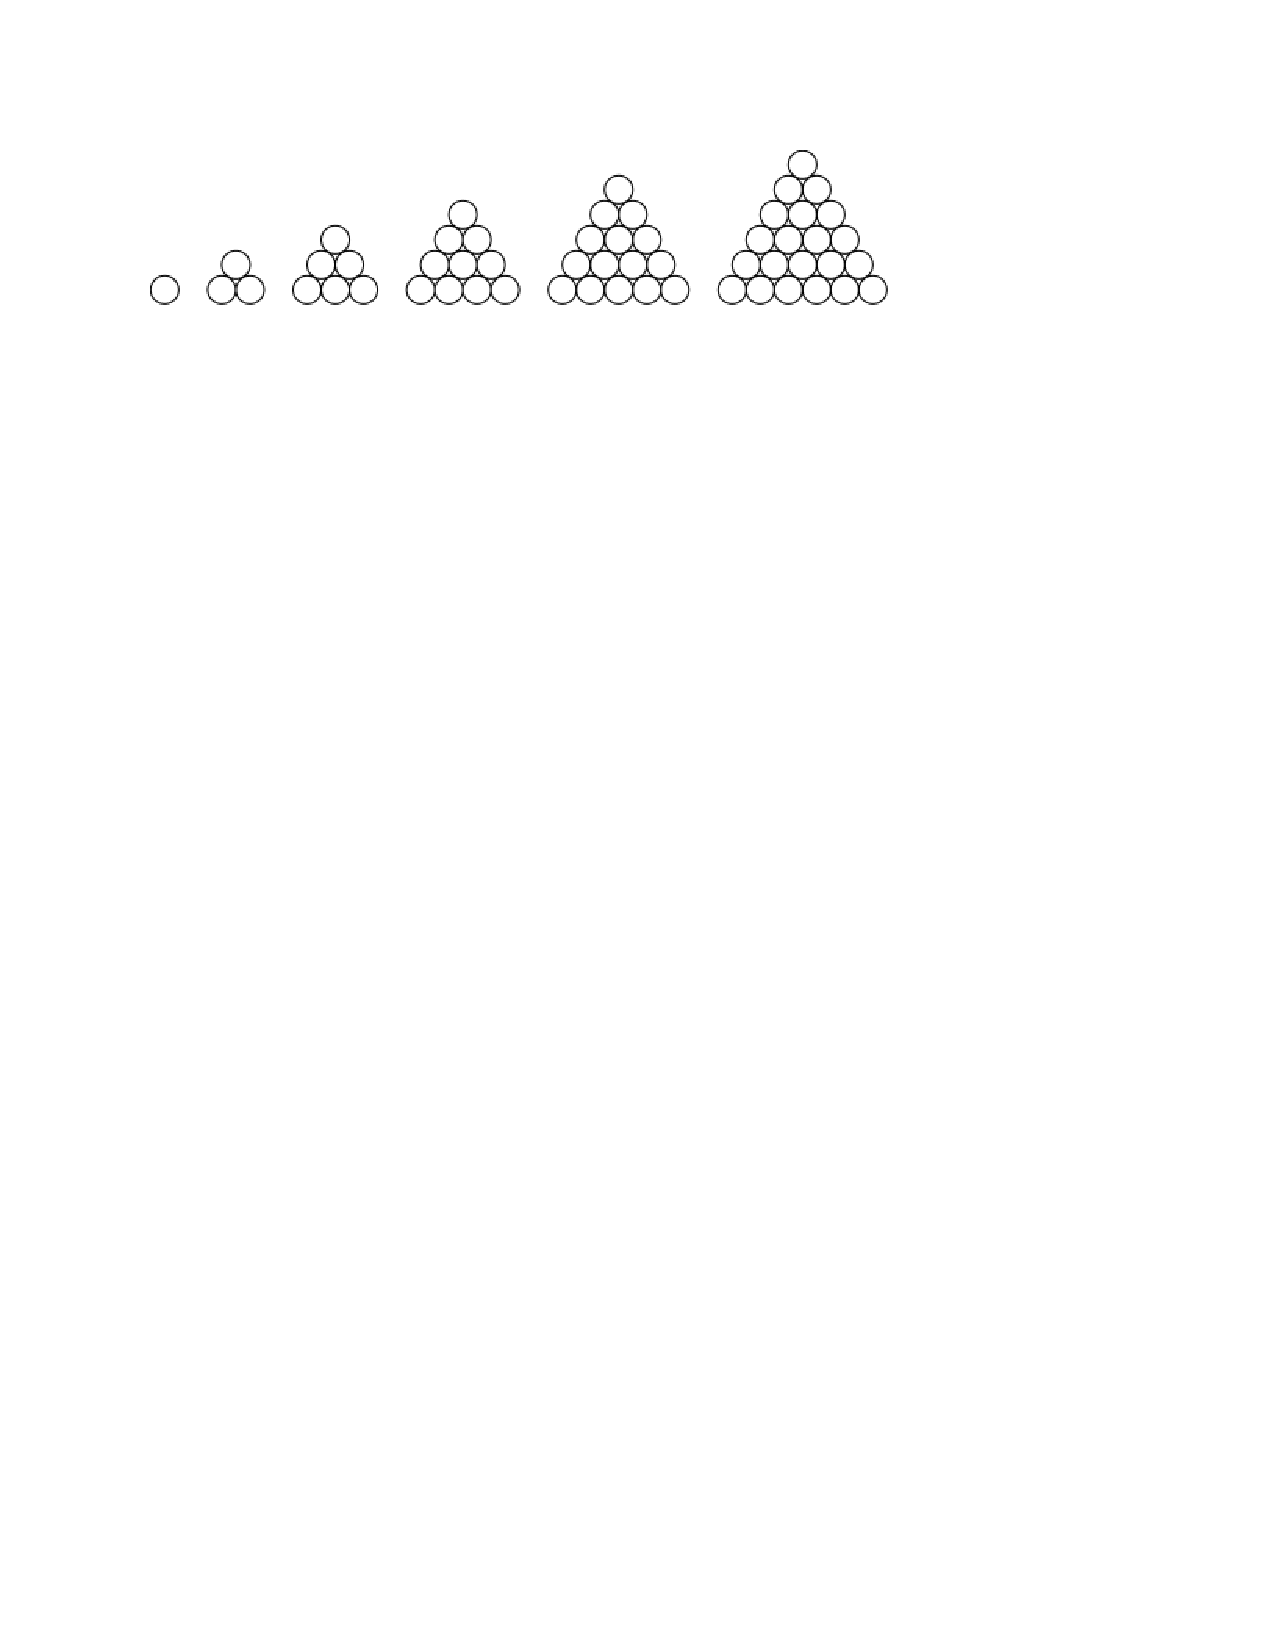
\includegraphics{../graphics/triangularNumbers}
\]
\fixnote{Need an original graphic here.}

\begin{prob}
Blair wanted to find the $551^{st}$ triangular number.  She used a table and looked for a pattern in the \emph{sequence of partial sums}:  $1, 1+2, 1+2+3, \dots$.  Help her finish her idea.  
\end{prob}

\begin{prob}
Kaley realized the the $551^{st}$ triangular number would be the sum 
\[
1+2+3+4+\dots+548+549+550+551
\]
She started pairing the first with the last number; the second with the second-to-last; the third with the third-to-last; and so on.  She saw that the averages are always the same.  Help her finish her idea.  
\end{prob}

\begin{prob}
Ali begin by writing out the sum forward and backward and follows:  
\[
\begin{array}{c@{ + }c@{ + }c@{ + }c@{ + }c@{ + }c@{ + }c@{ + }c@{ + }c@{ + }c@{ + }c@{ + }c@{ + }c}
1 & 2 & 3 & 4 & 5 & 6 & \cdots & 546 & 547 & 548 & 549 & 550 & 551 \\
551 & 550 & 549 & 548 & 547 & 546 & \cdots & 6 & 5 & 4 & 3 & 2 & 1 
\end{array}
\]
Help her finish her idea.  Be sure to explain clearly what happens ``in the dots.''  Does it matter whether there are an even or an odd number of terms?  
\end{prob}

\begin{prob}
Cooper was interested in a different triangular number and drew the following picture:   
\[
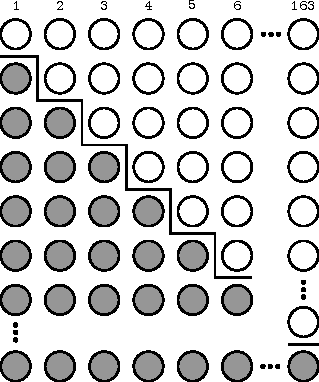
\includegraphics{../graphics/sum1.pdf}
\]
Which triangular number was he finding?  Help him finish his idea.  Be sure to explain clearly what 
happens ``in the dots.'' 
\end{prob}


\begin{prob}
Sum the numbers:  
\[
106 + 112 + 118 + \dots + 514
\]
\end{prob}

\begin{prob}
Sum the numbers:
\[
2.2 + 2.9 + 3.6 + 4.3 + \dots + 81.3
\]
\end{prob}


\begin{prob}
Suppose you have an arithmetic sequence beginning with $a$, with a constant difference of $d$ and with $n$ terms.  
\begin{enumerate}
\item What is the $n^{th}$ term of the sequence?  
\item Use dots to write the series consisting of the first $n$ terms of this sequence.
\item Find the sum of this series.  
\end{enumerate}
\end{prob}




\newpage
\section{Geometic Series}\label{A:geometicSeries}

In this activity, we explore \emph{geometric series}, which are sums of consecutive terms from an geometric sequence.

Ms. Radigan's math class has been trying to compute the following sums:  
$$1+2+4+8+\dots+2^{19}$$
$$\frac{2}{3}+\frac{2}{9}+\frac{2}{27}+\dots+\frac{2}{3^{13}}$$

\begin{prob}
Kelsey used tables and looked for pattern in the \emph{sequence of partial sums}:  $1, 1+2, 1+2+4, \dots$.  Help her finish her idea for both sequences.    
\end{prob}

\begin{prob}
For the sum beginning with $\frac{2}{3}$, Erin started by drawing a large square (which she imagined as having area 1), and she shaded in $\frac{2}{3}$ of it.  Then she shaded in $\frac{2}{9}$ more, and so on.  Help her finish her idea.  
\end{prob}

\begin{prob}
Ryan wrote out all of the terms in the first sum, represented as powers of 2, beginning with $1+2+2^2+2^3$.  
Then he realized that because the terms formed a geometric sequence, he could multiply the series by the common ratio of 2, and the resulting series would be almost identical to the first, differing only at the beginning and the end.  By subtracting the first series from the second, all of the middle terms would cancel.  Help him finish his idea.  
\end{prob}

\begin{prob}
Ali said, ``Here is a thought experiment.  I take a sheet of paper, rip it perfectly into thirds, place one piece to start a pile that I will call A, another piece to start a pile I will call B, and I keep the third piece in my hands.  I then rip that piece into thirds, place one piece on pile A, one piece on pile B, and keep the third.  Notice that each of pile A and pile B have $\frac{1}{3}+\frac{1}{9}$ of a sheet of paper, and I still have $\frac{1}{9}$ of a sheet in my hands.  I continue this process until I place $\frac{1}{3^{13}}$ of a sheet on each pile and still have $\frac{1}{3^{13}}$ of a sheet in my hands.  

Help Ali finish her idea.  
\end{prob}


\begin{prob}
Sum the expression:  
\[
\frac{2}{3}+\frac{4}{9}+\frac{8}{27}+\dots+\frac{2^n}{3^n}
\]
What happens to this sum as $n$ gets really large?  
\end{prob}


\begin{prob}
Consider the expression: 
$$\frac{7}{10}+\frac{7}{100}+\frac{7}{1000}+\dots+\frac{7}{10^n}$$
\begin{enumerate}
\item Find the sum of the expression. 
\item What happens to this sum as $n$ gets really large?  
\item How does this help you explain why a particular repeating decimal is a particular rational number?  Be sure to indicate what repeating decimal and what rational number you are talking about.  
\end{enumerate}
\end{prob}


\begin{prob}
Suppose you have an geometric sequence beginning with $a$, with a constant ratio of $r$ and with $n$ terms.  
\begin{enumerate}
\item What is the $n^{th}$ term of the sequence?  
\item Use dots to write the series consisting of the first $n$ terms of this sequence.
\item Find the sum of this series.  
\end{enumerate}
\end{prob}




%\newpage
\section{Second Differences}\label{A:secondDifferences}
In a previous activity, we developed strategies for finding the sum of arithmetic series.  In this activity, we use arithmetic series to develop a formula for a sequence that has constant second differences.  Then we demonstrate that all quadratic sequences have constant second differences.  

\begin{prob}
Consider the sequence $f(n)$ given in the table below.  In the rightmost column, $\Delta$ (``delta'') means difference, computed by subtracting the current value of $f(n)$ from the next.  
\vspace{0.1in} 
\[{\renewcommand{\arraystretch}{1.6}
\begin{tabular}{|c|c|c|}\hline
$n$ & $f(n)$ & $\Delta$ \\ \hline
   0     &  \cellcolor{lightgray}4  &  \cellcolor{lightgray}3  \\ \hline
   1     &  7 &   \cellcolor{lightgray}3 \\ \hline
   2     &  10 &  \cellcolor{lightgray}3  \\ \hline
   3     &  13 &  \cellcolor{lightgray}3  \\ \hline
   4     &  16 &  \cellcolor{lightgray}3   \\ \hline
   5     &  19 &    \\ \hline
\rule[5mm]{12mm}{0mm}  &  \rule[5mm]{12mm}{0mm} &\rule[5mm]{12mm}{0mm}    \\ \hline
\end{tabular}}
\]
\vspace{0.1in} 
\begin{enumerate}
\item Explain how $f(5)$ can be computed from the shaded cells in the table.  
\item Generalize your method to develop and explain a formula for $f(n)$.  
\item What was it about the differences that made this problem easy?  
\end{enumerate}
\end{prob}

\newpage

\begin{prob}
Consider the sequence $g(n)$ given in the table below.  
\vspace{0.1in} 
\[{\renewcommand{\arraystretch}{1.6}
\begin{tabular}{|c|c|c|c|}\hline
$n$ & $g(n)$ & $\Delta$ & $\Delta\Delta$ \\ \hline
   0     &  \cellcolor{lightgray}1  &  \cellcolor{lightgray}  & \\ \hline
   1     &  $-2$ &  \cellcolor{lightgray} & \\ \hline
   2     &  1 &  \cellcolor{lightgray}  & \\ \hline
   3     &  10 &  \cellcolor{lightgray} &  \\ \hline
   4     &  25 & \cellcolor{lightgray}  &  \\ \hline
   5     &  46 &   &  \\ \hline
   6     &  73 &   &  \\ \hline
\rule[5mm]{12mm}{0mm}  &  \rule[5mm]{12mm}{0mm} &\rule[5mm]{12mm}{0mm}  &\rule[5mm]{12mm}{0mm}   \\ \hline
\end{tabular}}
\]
\vspace{0.1in} 
\begin{enumerate}
\item Compute $\Delta$ by subtracting the current value of $g(n)$ from the next.  
\item Explain the formula $\Delta(n) = g(n+1)-g(n)$.
\item Check that the shaded cells sum to $g(5)$, and explain how that makes sense based upon how the $\Delta$ values were calculated.  \item Because the $\Delta$ values (``first differences'') are not constant, use the $\Delta\Delta$ column to compute the ``differences of the differences'' (also called ``second differences'').  
\item From the fact that the second differences are constant, develop an explicit formula for $\Delta$ in terms of $n$.  
\end{enumerate}
\end{prob}

\newpage

\begin{prob}
The same sequence $g(n)$ is given below, this time with a formula for $\Delta$ in terms of $n$.    
\vspace{0.1in} 
\[{\renewcommand{\arraystretch}{1.6}
\begin{tabular}{|c|c|c|}\hline
$n$ & $g(n)$ & $\Delta(n)=6n-3$  \\ \hline
   0     &   \cellcolor{lightgray}1  &   \cellcolor{lightgray}$-3$  \\ \hline
   1     &  $-2$ &  \cellcolor{lightgray}3   \\ \hline
   2     &  1 &    \cellcolor{lightgray}9  \\ \hline
   3     &  10 &  \cellcolor{lightgray}15    \\ \hline
   4     &  25 &   \cellcolor{lightgray}21   \\ \hline
   5     &  46 &  27   \\ \hline
   6     &  73 &     \\ \hline
\rule[5mm]{12mm}{0mm}  &  \rule[5mm]{12mm}{0mm} &\rule[5mm]{12mm}{0mm}    \\ \hline
\end{tabular}}
\]
\vspace{0.1in} 
\begin{enumerate}
\item Explain each of the following steps:    
\begin{align*}
g(5) &= 1 + \Delta(0) + \Delta(1) + \Delta(2) + \Delta(3) + \Delta(4)  \\
        &= 1 + (6\cdot 0 -3) + (6\cdot1 -3) + (6\cdot2 -3) + (6\cdot3 -3) + (6\cdot4 -3) \\
        & = 1 + 6\cdot( 0 + 1 + 2 + 3 + 4) + (-3 + -3 + -3 + -3 + -3) \\
        & = 1 + 6\cdot\frac{5\cdot 4}{2} + 5\cdot (-3)
\end{align*}
\item Where do you see arithmetic series in the calculations you just explained?  
\item Generalize the above approach to yield an expression for $g(n)$.  
\item What kind of sequence is $g(n)$?  
\end{enumerate}

\end{prob}

\newpage

\begin{prob}
A general quadratic sequence $h(n)$ is given below.    
\vspace{0.1in} 
\[{\renewcommand{\arraystretch}{1.6}
\begin{tabular}{|c|c|c|c|}\hline
$n$ & $h(n)=an^2+bn+c$ & $\Delta$ & $\Delta\Delta$ \\ \hline
   0     &    &    & \\ \hline
   1     &   &   & \\ \hline
   2     &   &    & \\ \hline
   3     &   &   &  \\ \hline
\rule[5mm]{12mm}{0mm}  &  \rule[5mm]{12mm}{0mm} &\rule[5mm]{30mm}{0mm}  &\rule[5mm]{30mm}{0mm}   \\ \hline
\end{tabular}}
\]
\vspace{0.1in} 
\begin{enumerate}
\item Compute the values of $h(n)$.  
\item Compute $\Delta$ by subtracting the next value of $h(n)$ from the current.  
\item Use the $\Delta\Delta$ column to compute the second differences.  
\item Generalize the result for first differences by computing $\Delta(n)=h(n+1)-h(n)$.
\item Generalize the result for second differences by computing $\Delta\Delta(n)=\Delta(n+1)-\Delta(n)$.
\item Explain how your work demonstrates that, for any quadratic sequence, the second differences must be constant.  
\end{enumerate}
\end{prob}

   % Requires \RequirePackage{xcolor,colortbl}, but then some of the Euclidean Algorithm sections won't compile.  

\newpage
\section{Hieroglyphical Algebra}\label{A:HAlgebra} 
\symbolfootnote[0]{This activity is based on an activity originally designed by Lee Wayand.}

Consider the following addition and multiplication tables:
\[
{\renewcommand{\arraystretch}{1.8}
\begin{array}{clc}
{\renewcommand{\arraystretch}{1.8}
\begin{array}{|c||c|c|c|c|c|c|c|c|c|}\hline
 +  &\loo & \la & \lo & \lb & \lc & \ld & \lf & \lh & \li \\ \hline\hline
\loo& \ld & \lh &\loo & \li & \lb & \lo & \la & \lf & \lc \\ \hline
\la & \lh & \li & \la & \ld &\loo & \lf & \lb & \lc & \lo \\ \hline
\lo &\loo & \la & \lo & \lb & \lc & \ld & \lf & \lh & \li \\ \hline
\lb & \li & \ld & \lb & \lh & \la & \lc &\loo & \lo & \lf \\ \hline
\lc & \lb &\loo & \lc & \la & \lf & \li & \lo & \ld & \lh \\ \hline
\ld & \lo & \lf & \ld & \lc & \li &\loo & \lh & \la & \lb \\ \hline
\lf & \la & \lb & \lf &\loo & \lo & \lh & \lc & \li & \ld \\ \hline
\lh & \lf & \lc & \lh & \lo & \ld & \la & \li & \lb &\loo \\ \hline
\li & \lc & \lo & \li & \lf & \lh & \lb & \ld &\loo & \la \\ \hline
\end{array}}
\vspace{.5cm}
& 
\begin{array}{l}
\text{$\loo =$ fish} \\ 
\text{$\la =$ lolly-pop} \\ 
\text{$\lo =$ skull} \\ 
\text{$\lb =$ cinder-block} \\ 
\text{$\lc =$ DNA} \\ 
\text{$\ld =$ fork} \\ 
\text{$\lf =$ man} \\ 
\text{$\lh =$ balloon} \\ 
\text{$\li =$ eyeball} 
\end{array}
& 
{\renewcommand{\arraystretch}{1.8}
\begin{array}{|c||c|c|c|c|c|c|c|c|c|}\hline
\cdot & \ld & \li & \lh & \lf & \lo & \la & \lb & \lc &\loo \\ \hline\hline
\ld   &\loo & \la & \lb & \lc & \lo & \li & \lh & \lf & \ld \\ \hline
\li   & \la & \lh & \lf & \ld & \lo & \lb & \lc &\loo & \li \\ \hline
\lh   & \lb & \lf & \ld & \la & \lo & \lc &\loo & \li & \lh \\ \hline
\lf   & \lc & \ld & \la & \lb & \lo &\loo & \li & \lh & \lf \\ \hline
\lo   & \lo & \lo & \lo & \lo & \lo & \lo & \lo & \lo & \lo \\ \hline
\la   & \li & \lb & \lc &\loo & \lo & \lh & \lf & \ld & \la \\ \hline
\lb   & \lh & \lc &\loo & \li & \lo & \lf & \ld & \la & \lb \\ \hline
\lc   & \lf &\loo & \li & \lh & \lo & \ld & \la & \lb & \lc \\ \hline
\loo  & \ld & \li & \lh & \lf & \lo & \la & \lb & \lc &\loo \\ \hline
\end{array}} 
\end{array}}
\]

\newpage



\begin{prob} 
Can you tell me which glyph represents $0$? How did you arrive at this
conclusion?
\end{prob}

\begin{prob} 
Can you tell me which glyph represents $1$? How did you arrive at this
conclusion?
\end{prob}

\begin{prob}
A number $x$ has an \textit{additive inverse} if you can find another number $y$ with 
\[
x + y = 0.
\]
and we say that ``$y$ is the additive inverse for $x$.'' If possible,
find the additive inverse of every number in the table above.
\end{prob}

\begin{prob}
A number $x$ has a \textit{multiplicative inverse} if you can find
another number $y$ with
\[
x\cdot y = 1.
\]
and we say that ``$y$ is the multiplicative inverse for $x$.'' If
possible, find the multiplicative inverse of every number in the
table above.
\end{prob}



\begin{prob} If possible, solve the following equations:
\begin{enumerate}
\item $\lh \cdot \lx - \lb = \ld$
\item $\dfrac{\ly}{\lb} = \dfrac{\ld}{\loo}$
\item $\bigg(\lz - \ld\bigg)\bigg(\lz + \lf\bigg)=\loo$
\item $\dfrac{\loo - \lw}{\lc} + \ld = \dfrac{\lh}{\lf}$
\end{enumerate}
In each case explain your reasoning.
\end{prob}

\begin{prob} If possible, solve the following equations:
\begin{enumerate}
\item $\lx \cdot \lx = \ld$
\item $\lz\cdot \lz = \lf$
\item $\ly\cdot \ly + \ly \cdot \lb = \loo$
\item $\lw \cdot \lw+ \lc = \lw$
\end{enumerate}
In each case explain your reasoning.
\end{prob}



\newpage
\section{The Other Side---Solving Equations}\label{A:otherSide}


In this activity, we will explore ideas related to solving equations.

\begin{prob}
Solve the following equation three ways: Using algebra, using the
balance, and with the graph. At each step, the three models should be in
complete alignment.
\[
\]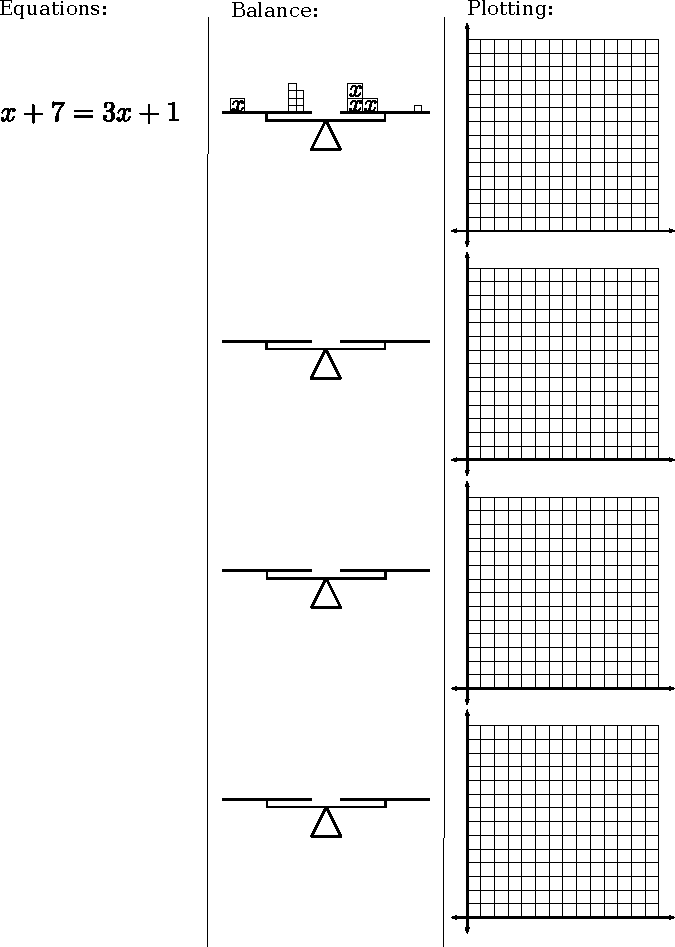
\includegraphics[scale=0.8]{../graphics/eqBalGraph.pdf}

\end{prob}

\begin{prob}
Critically analyze the three ``different'' methods of solving
equations. Can you solve quadratic equations using the methods above?
If so give an example. If not, explain why not.
\end{prob}

\begin{teachingnote}
The key point here is that it is difficult to make ``balances'' work
for anything but linear equations.
\end{teachingnote}



\begin{prob}
Can you think of an example when the undoing via algebraic
manipulation would fail?
\end{prob}

\begin{teachingnote}
Here we are looking for something where an inverse function must be
applied, as in $.6 = \sin(x)$.
\end{teachingnote}


While sometimes we solve equations via a process of algebraic
manipulation, other times we have a formula.


\begin{prob}
Give a formula for solving linear equations of the form $ax + b =0$.
\end{prob}

\fixnote{Incorporate the zero-product property somewhere.}

\begin{prob}
Complete the square to give a formula for solving equations of the form
\[
x^2 + bx + c = 0.
\]
\end{prob}


Of course these formulas can only take us so far. The key to solving
polynomial equations is that finding any root will allow you to
divide, and lower the degree.

\begin{prob}
Solve the following equation
\[
x^5 - 4x^4 - 18x^3 + 64x^2 + 17x -60 = 0
\]
assuming you know that $1$, $-1$, and $3$ are roots.
\end{prob}




\newpage
\section{Solving Quadratics}\label{A:solvingQuadratics}
\fixnote{Separate into two activities.  This is too much for one day.  Aim to complete through problem 8 on day 1.}
Here we explore various methods for solving quadratic equations in one variable.  \textbf{Please read all instructions carefully.}

\begin{prob}
Is $\sqrt{4}=\pm 2$?  Explain. 
\end{prob}

\vfill

\begin{teachingnote}
Both $2$ and $-2$ are ``square roots'' of $4$ because $2^2=4$ and $(-2)^2=4$, and both of them are solutions to the equation $x^2=4$.  The question is whether the radical symbol refers to both of them, either of them (you choose?), or a specific one of them.  
\end{teachingnote}

\begin{prob}
Suppose that $\sqrt{4}=\pm 2$?  Then evaluate $\sqrt{4}+\sqrt{9}$.  
\end{prob}

\begin{teachingnote}
$$\sqrt{4}+\sqrt{9}=\pm2+\pm3=5, -1, 1, or -5$$
\end{teachingnote}

\vfill

\begin{prob}
What does your calculator say about $\sqrt{4}+\sqrt{9}$?  
\end{prob}

\vfill 

\begin{teachingnote}
Now emphasize the conventional meaning of the radical symbol:  For $a>0$ then $\sqrt{a}$ means the positive square root of $a$.  
\end{teachingnote}



\begin{prob}
In the following problems, you \textbf{may not use the quadratic formula}.  But just for the record, write down the quadratic formula.  
\end{prob}
\begin{teachingnote}
Many students will write only $\frac{-b\pm\sqrt{b^2-4ac}}{2a}$, but we want them to write the following:  

$$\text{If }ax^2+bx+c=0\text{ and }a\ne 0\text{, then }x=\frac{-b\pm\sqrt{b^2-4ac}}{2a}\text{.}$$
Note that if the radical symbol were to refer to both a positive and negative square root, then there would be no reason to write $\pm$ outside the radical symbol.  
\end{teachingnote}

\vfill

\newpage

\begin{prob}
In the following list of equations, solve those that are \textbf{easy} to solve.  
\begin{enumerate}
\item $(x-3)(x+2)=0$
\item $(x-3)(x+2)=1$
\item $(2x-5)(3x+1)=0$
\item $(x-a)(x-b)=0$
\item $(x-1)(x-3)(x+2)(2x-3)=0$
\end{enumerate}
\end{prob}

\begin{prob}
Regarding the previous problem, state the property of numbers that made all but one of the equations easy to solve.  
\end{prob}

\begin{teachingnote}
Zero product property:  If $ab = 0$ then $a=0$ or $b=0$.  Note that this doesn't work when the right side is not 0.  
\end{teachingnote}

\vspace{0.3in}


%\begin{prob} For each part below, write a linear equation with the state solution.  
%\begin{enumerate}
%\item $x=\frac{2}{3}$
%\item $x=\frac{a}{b}$
%\end{enumerate}
%\end{prob}

\begin{prob}For each part below, write a quadratic equation with the stated solution(s) and no other solutions.  
\begin{enumerate}
\item $x=7$ or $x=-4$
\item $x=p$ or $x=q$
\item $x=3$
\item $x=\frac{1\pm\sqrt{5}}{2}$
 \end{enumerate}
\end{prob}

\begin{teachingnote}
In the following problem, discuss ways of explaining that 
$$\pm\sqrt{\frac{1}{2}}=\pm\frac{1}{\sqrt{2}}=\pm\frac{\sqrt{2}}{2}$$
\end{teachingnote}

\begin{prob}
In the following list of equations, solve those that are \textbf{easy} to solve.  
\begin{enumerate}
\item $x^2=5$
\item $x^2 - 4 = 2$
\item $x^2 - 4x = 2$
\item $2x^2=1$
\item $(x-2)^2=5$
\end{enumerate}
\end{prob}
\vspace{0.3in}

\begin{prob}
Regarding the previous problem, state the property of numbers that made all but one of the equations easy to solve.  
\end{prob}
\vspace{0.3in}

\begin{teachingnote}
If $u^2=a$ then $u=\pm\sqrt{a}$.
\end{teachingnote}

\begin{prob}
Although $160$ is not a square in base ten, what could you add to $160$ so that the result would be a square number?  
\end{prob}

\begin{prob}
 Consider the polynomial expression $x^2+6x$ to be a number in base $x$.  We want to add to this polynomial so that the result is a square in base $x$.  
\begin{enumerate}
\item Use ``flats'' and ``longs'' to draw a picture of this polynomial as a number in base $x$, adding enough ``ones'' so that you can arrange the polynomial into a square.  
\vspace{0.5in}
\item What ``feature'' of the square does the new polynomial expression represent?  
\item Why does it make sense to call this technique ``completing the square''? 
\item Use your picture to help you solve the equation $x^2+6x=5$.  
\end{enumerate}
\end{prob}

\newpage

\begin{prob}
Complete the square to solve the following equations: 
\begin{enumerate}
\item $x^2+3x=4$
\vspace{.8in}
\item $x^2+bx=q$
\vspace{.8in}
\item $2x^2+8x=12$
\vspace{.8in}
\item $ax^2+bx+c=0$
\vspace{.8in}
\end{enumerate}  
\end{prob}

\fixnote{Perhaps delete the rest of the problems or move them elsewhere.}
\begin{prob}
Find all solutions to $x^3-3x^2+x+1=0$.  Hint:  One solution is $x=1$.  
\end{prob}

\begin{prob}
Solve the following equation
\[
x^5 - 4x^4 - 18x^3 + 64x^2 + 17x -60 = 0
\]
assuming you know that $1$, $-1$, and $3$ are roots.
\end{prob}



\newpage
\section{Complete Squares}\label{A:completeSquares}

\begin{prob}
In the following list of equations, solve those that are \textbf{easy} to solve.  
\begin{enumerate}
\item $x^2=5$
\item $x^2 - 4 = 2$
\item $x^2 - 4x = 2$
\item $2x^2=1$
\item $(x-2)^2=5$
\end{enumerate}
\end{prob}
\vspace{0.3in}

\begin{prob}
Regarding the previous problem, state the property of numbers that made all but one of the equations easy to solve.  
\begin{teachingnote}
If $u^2=a$ then $u=\pm\sqrt{a}$.  Be sure to spend some time discussing why 
$$\pm\sqrt{\frac{1}{2}}=\pm\frac{1}{\sqrt{2}}=\pm\frac{\sqrt{2}}{2}.$$
\end{teachingnote}
\vspace{0.3in}
\end{prob}

\begin{prob}
Although $160$ is not a square in base ten, what could you add to $160$ so that the result would be a square number?  
\end{prob}

\begin{prob}
 Consider the polynomial expression $x^2+6x$ to be a number in base $x$.  We want to add to this polynomial so that the result is a square in base $x$.  
\begin{enumerate}
\item Use ``flats'' and ``longs'' to draw a picture of this polynomial as a number in base $x$, adding enough ``ones'' so that you can arrange the polynomial into a square.  
\vspace{0.5in}
\item What ``feature'' of the square does the new polynomial expression represent?  
\item Why does it make sense to call this technique ``completing the square''? 
\item Use your picture to help you solve the equation $x^2+6x=5$.  
\end{enumerate}
\end{prob}


\begin{prob}
Complete the square to solve the following equations: 
\begin{enumerate}
\item $x^2+3x=4$
\vspace{.8in}
\item $x^2+bx=q$
\vspace{.8in}
\item $2x^2+8x=12$
\vspace{.8in}
\item $ax^2+bx+c=0$
\vspace{.8in}
\end{enumerate}  
\end{prob}

\begin{prob}
Solve the following equation
\[
x^5 - 4x^4 - 18x^3 + 64x^2 + 17x -60 = 0
\]
assuming you know that $1$, $-1$, and $3$ are roots.
\end{prob}



\newpage
\section{Maximums and Minimums}\label{A:vertex}

\begin{teachingnote}
This activity will be necessary for computing least squares
approximation.
\end{teachingnote}


While you might have encountered completing the
square\index{completing the square} first when solving quadratic
equations, its real power is in transforming the form of an
expression. In this activity, we'll see it in action.

\begin{prob}
Consider the curve $f(x) = x^2 -3$. Find the $x$ and $y$ values for
the maximum/minimum value(s) of this curve. Explain how you know you
are correct.
\end{prob}

\begin{prob}
Consider the curve $f(x) = 3(x-5)^2 +7$. Find the $x$ and $y$ values for
the maximum/minimum value(s) of this curve. Explain how you know you
are correct.
\end{prob}



\begin{prob}
Consider the curve $f(x) = -2(x+3)^2 + 7$. Find the $x$ and $y$ values for
the maximum/minimum value(s) of this curve. Explain how you know you
are correct.
\end{prob}

\begin{prob}
What type of curve is drawn by $f(x) = a(x-h)^2+k$? Find the $x$ and
$y$ values for the maximum/minimum value(s) of this curve. Explain how
you know you are correct.
\end{prob}

\begin{teachingnote}
This is the vertex form of a parabola.
\end{teachingnote}


\begin{prob}
Consider the parabola $f(x) = x^2 + 4x + 2$. Complete the square to
put this expression in the form above and identify the maximum/minimum
value(s) of this curve.
\end{prob}


\begin{prob}
Consider the parabola $f(x) = 2x^2 - 8x + 6$. Complete the square to
put this expression in the form above and identify the maximum/minimum
value(s) of this curve.
\end{prob}

\begin{prob}
Consider the parabola $f(x) = 3x^2 + 7x - 1$. Complete the square to
put this expression in the form above and identify the maximum/minimum
value(s) of this curve.
\end{prob}


\begin{prob}
Given a parabola $f(x) = ax^2 + bx +c$. Complete the square to put
this expression in the form above and identify the maximum/minimum
value(s) of this curve.
\end{prob}


\begin{prob}
Could you find the same formula found in the previous question by
appealing to the symmetry of the roots?
\end{prob}







%\newpage
\section{Least Squares Approximation}\label{A:leastSquares}

In this activity, we are going to investigate \textit{least
squares approximation}\index{least squares approximation}.

\begin{prob}
Consider the following data:
\{(2,3), (4,5), (6,11)\}
\[

\includegraphics{../graphics/complexPlane.pdf}
\]
Plot the data and use a ruler to sketch a ``best fit'' line.
\end{prob}

\begin{prob}
Now we are going to record some more data in the chart below:
\begin{enumerate}
\item  For each data point, use a ruler to measure the vertical distance between the point and the line. Record this in the first empty row of the table below.
\item For each data point, square the vertical distance. Record this in the second empty row of the table below.
\end{enumerate}
\[
{\renewcommand{\arraystretch}{1.8}
\renewcommand{\arraycolsep}{3mm}
\begin{array}{|l||c|c|c|c|}\hline
\text{Point} & (2,3) & (4,5) & (6,11)  \\ \hline\hline
\text{Vertical Distance} & & & \\ \hline
\text{Squares} & & & \\ \hline
\end{array}}
\]
\end{prob}

\begin{prob}
Add up the squares of the vertical distances. You want this to be as
small as possible. Compare your sum with that of a friend, or enemy.
Whoever got the smallest value has the best approximation of the given data.
\end{prob}

\begin{prob}
Now find the equation of the line you drew. Write it down and don't
forget it!
\end{prob}

So far we've just been ``eye-balling'' our data. Let's roll up our
sleaves and do some real math.

\begin{prob}
Suppose that your line is $\l(x) = ax + b$. Give an expression
representing the sum of squares you get with your data above.
\end{prob}

\begin{teachingnote}
Here we're looking for something like:
\[
(a\cdot 2+ b -3)^2 + (a\cdot 4+ b -5)^2 + (a\cdot 6+ b -11)^2
\]
\end{teachingnote}

\begin{prob}
Simplfy the expression above. You should now have a quadratic in two
variables $a$ and $b$. Find the minimum, thinking of this as quadratic equation in $a$ and then thinking of this as a quadratic equation in $b$. 
\end{prob}

\begin{prob}
You should now have two equations, and two unknowns---solve!
\end{prob}


\begin{prob}
Compare your computed formula with the line you guessed---how did you
do?
\end{prob}


\newpage
\section{Solving Cubic Equations}\label{A:solvingCubics}

To solve the cubic equation $x^3+px+q=0$, we use methods that were discovered and advanced by various mathematicians, including Ferro, Tartaglia, and Cardano.  The approach is organized in three steps.  \textbf{Make notes in the margin as you follow along.}  

%\begin{itemize}
%\item Step 1:  Replace $x$ with $u+v$.
%\item Step 2: Set $uv$ so that all of the terms are eliminated except for $u^3$, $v^3$, and constant terms.
%\item Step 3: Clear denominators, recognize the equation as a quadratic in $u^3$, and use the quadratic formula.
%\end{itemize}

\subsection{Step 1:  Replace $x$ with $u+v$}
In $x^3+px+q=0$, let $x = u + v$.  % $$(u+v)^3+p(u+v)+q=0.$$ 
Show that the result can be written as follows:  

$$u^3+v^3+(3uv+p)(u+v)+q = 0.$$

\subsection{Step 2: Set $uv$ to eliminate terms}
If $3uv+p=0$, then all of the terms are eliminated except for $u^3$, $v^3$, and constant terms. Explain why the equation simplifies nicely to:

$$u^3+v^3 + q = 0.$$

Solve $3uv+p=0$ for $v$, substitute, and show that we have:  

$$u^3+\left( \frac{-p}{3u}\right)^3+q=0.$$

\subsection{Step 3:  Recognize the equation as a quadratic in $u^3$ and solve}

By multiplying by $u^3$, show that we get a quadratic in $u^3$:   

$$u^6+qu^3+\left( \frac{-p}{3}\right)^3 = 0.$$

Show that this has solutions: 

$$u^3 = \frac{-q\pm\sqrt{q^2-4\left( \frac{-p}{3}\right)^3}}{2}.$$

Now, use the facts $v= -p/(3u)$ and $x = u + v$ to write a formula for $x$: 

$$x = \sqrt[3]{\frac{-q\pm\sqrt{q^2-4\left( \frac{-p}{3}\right)^3}}{2}} 
+  \frac{-p}{3\sqrt[3]{\frac{-q\pm\sqrt{q^2-4\left( \frac{-p}{3}\right)^3}}{2}}}.$$

\begin{prob}
How many values does this formula give for $x$?  From the original equation $x^3+px+q=0$, how many solutions should we expect? 
\end{prob}
\vfill

\begin{prob}
Use the above formula to solve the specific equation $x^3-15x-4=0$.  Show that $$x = \sqrt[3]{2 \pm \sqrt{-121}} + \frac{5}{\sqrt[3]{2\pm\sqrt{-121}}}.$$
Are these values of $x$ real numbers?  
\end{prob}
\vfill


\begin{prob}
Use technology to graph $y=x^3-15x-4$.  According to the graph, how many real roots does the polynomial have?  What is going on?  
\end{prob}
\vfill

\begin{prob}
Choose ``plus'' in the $\pm$, and check that $2+\sqrt{-1}$ is a cube root of $2 + \sqrt{-121}$.  Use that fact to simplify the above expression for $x$.  What do you notice?  
\end{prob}
\vfill

\begin{prob}
Now choose ``minus'' in the $\pm$ above, and find the value of $x$.  What do you notice?  
\end{prob}

\vfill
In both cases, the formula requires computations with square roots of negative numbers, but the result is a real solution.  These kinds of occurrences were the historical impetus behind the gradual acceptance of complex numbers.  



%\newpage
\section{It Takes All Kinds\dots}\label{A:otherCurves}
\fixnote{Maybe move these to problems.  Replace with linear, quadratic, exponential sheet.}

Data can come in all shapes and sizes. While a line is the simplest
approximation, it might not be the best.

\begin{prob}
Consider the data below:
\[
\begin{array}{|c|c|c|c|c|}\hline
x & 0 & 1 & 2 & 3 \\ \hline
y & 8.1 & 22.1 & 60.1 & 165 \\ \hline
\end{array}
\]
What type of data is this? To get the ``brain
juices'' flowing here are some choices. It could be:
\begin{enumerate}
\item A parabola.
\item An exponential.
\item A quartic.
\item Something else.
\end{enumerate}
Hint: Think about the most famous graph of all, the one you know most
about.  And see if you can somehow convert the above data to get that
type of graph. You will probably need to make some plots. 
\end{prob}


\begin{prob}
Now do the same with this data:
\[
\begin{array}{|c|c|c|c|c|}\hline
x & 1 & 2 & 3 & 4 \\ \hline
y & 8.3 & 443.6 & 24420.8 & 1364278.6 \\ \hline
\end{array}
\]
\end{prob}


\begin{prob}
Now do the same with this data:
\[
\begin{array}{|c|c|c|c|c|c|}\hline
x & 1 & 2 & 3 & 4 & 5 \\ \hline
y & 7 & 62 & 220 & 506 & 1012 \\ \hline 
\end{array}
\]
\end{prob}

\begin{prob}
Here is a sample of semi-log paper. What's going on here?
\[
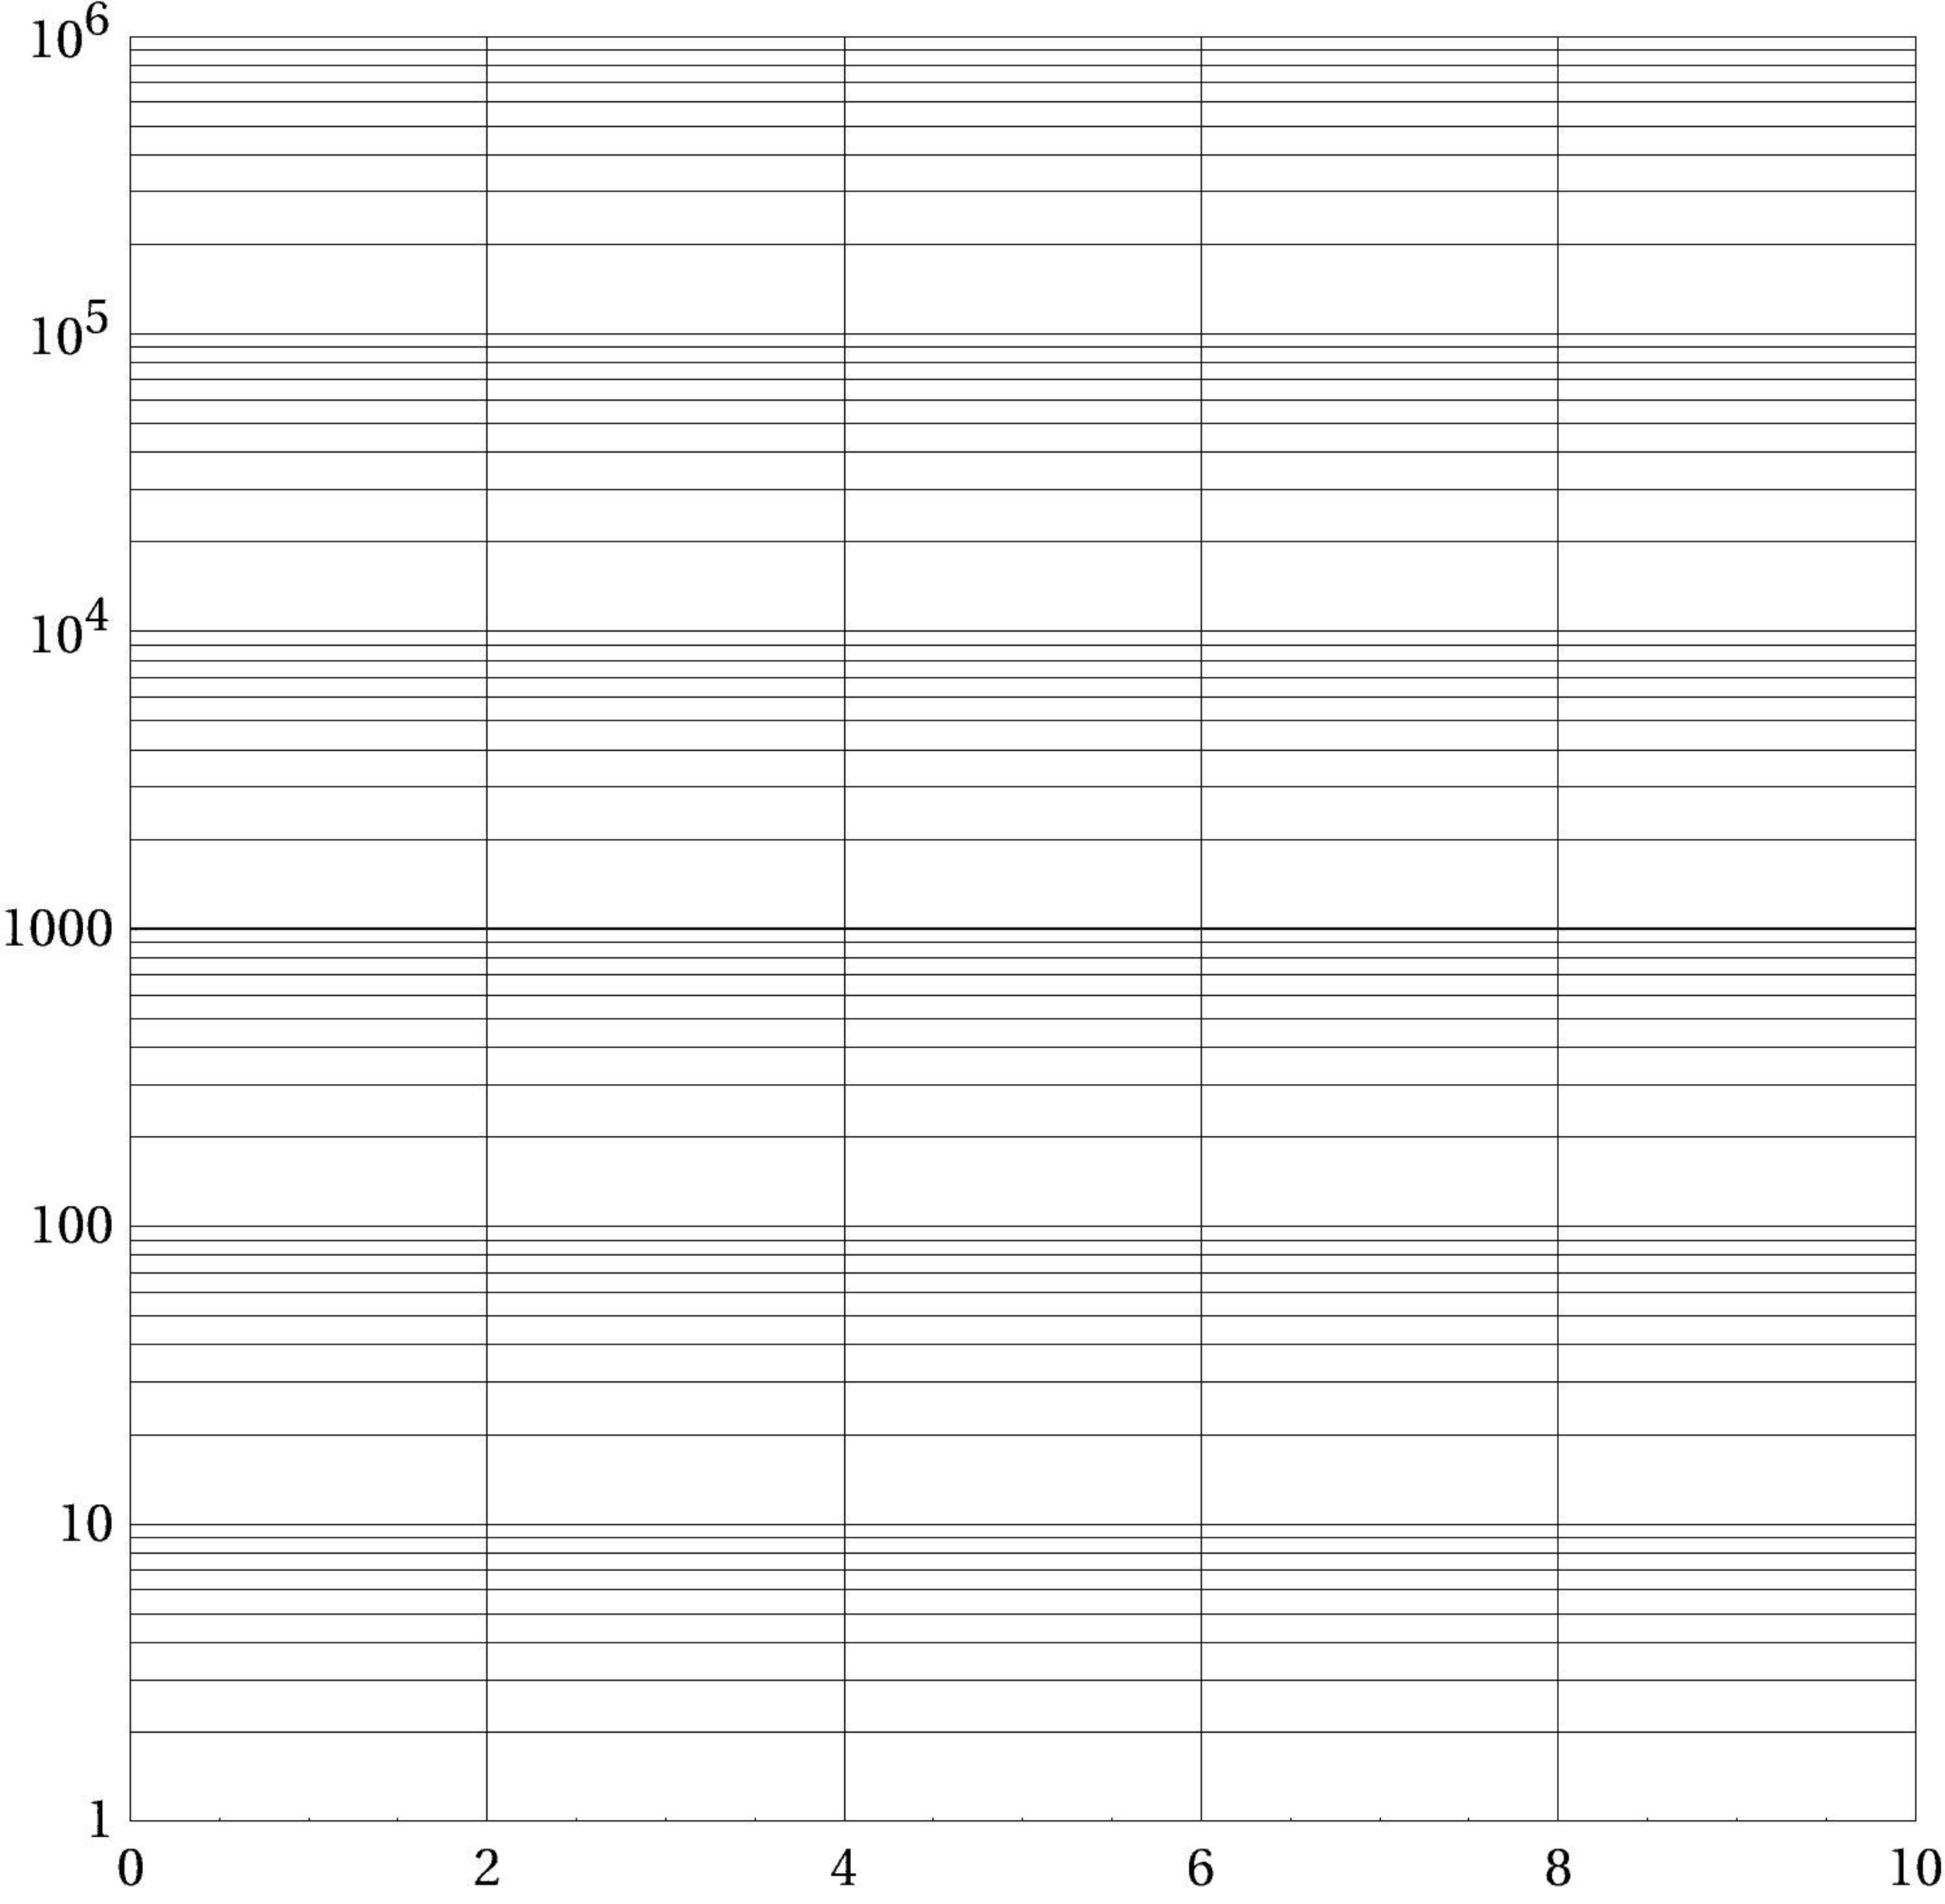
\includegraphics[width=4in]{../graphics/semiLog.pdf}
\]
\end{prob}


\newpage
\section{Sketching Roots}\label{A:sketchRoots}

In this activity we seek to better understand the connection between
roots and the plots of polynomials.  First, we need to be precise about the correct usage of some important language:  

\begin{itemize}
\item Expressions have \emph{values}.  
\item Equations have \emph{solutions}:  values of the variables that make the equation true. 
\item Functions have \emph{zeros}: input values that give output values of 0.
\item Polynomials (i.e., polynomial expressions) have \emph{roots}.  
\end{itemize}
These ideas are related, of course, as follows:  A zero of a polynomial function, p(x), is a root of the polynomial p(x) and a solution to the equation p(x) = 0.  

Please try to use this language correctly:  Equations do not have zeros, and functions do not have solutions.  

\begin{prob}
Give an example of a polynomial, and write a true sentence about related equations, functions, zeros, equations, and roots.  
\end{prob}

\begin{prob}
Sketch the plot of a quadratic polynomial with real coefficients that has:
\begin{enumerate}
\item Two real roots.
\item One repeated real root.
\item No real roots.
\end{enumerate}
In each case, give an example of such a polynomial.
\end{prob}

\begin{prob}
Can you have a quadratic polynomial with exactly one real root and
$1$ complex root?  Explain why or why not.
\end{prob}


\begin{prob}
Sketch the plot of a cubic polynomial with real coefficients that has:
\begin{enumerate}
\item Three distinct real roots.
\item One real root and two complex roots.
\end{enumerate}
In each case, give an example of such a polynomial.
\end{prob}

\begin{prob}
Can you have a cubic polynomial with no real roots?  Explain why or
why not. What about two distinct real roots and one complex root?
\end{prob}


\begin{prob}
For polynomials with real coefficients of degree $1$ to $5$, classify
exactly which types of roots can be found. For example, in our work
above, we classified polynomials of degree $2$ and $3$.
\end{prob}


\newpage
\section{Geometry and Adding Complex Numbers}\label{A:complexAddition}


Let's think about the geometry of adding complex numbers. We won't be
alone on our journey---Louie Llama\index{Louie Llama} is here to help
us out:
\[
\begin{tabular}{ccc}

\includegraphics[scale=.5]{../graphics/llama.pdf} & \qquad $\leftrightsquigarrow$\qquad& 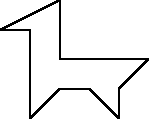
\includegraphics{../graphics/llamaPlot.pdf}\\
Louie Llama & & how we'll draw him
\end{tabular}
\]

\begin{prob} 
Here's Louie Llama hanging out near the point $0$ in the complex
plane. Add $4+4i$ to him. Make a table and show in the plane below what happens.
\[
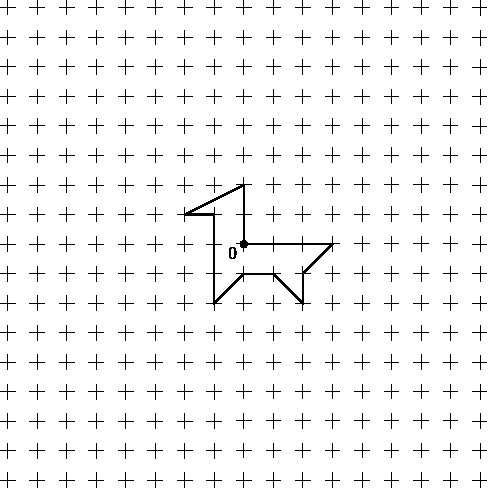
\includegraphics{../graphics/complexAdd.pdf}
\]
\end{prob}

\begin{prob}
Explain what it means to ``add'' a complex number to Louie
Llama. Describe the process(es) used when doing this.
\end{prob}


\begin{prob} 
Put Louie Llama back where he started, now add $1-5i$ to him.  Make a
table and show what happens in the plane.
\end{prob}


\begin{prob} 
Geometrically speaking, what does it mean to ``add'' complex numbers?
\end{prob}


\newpage
\section{Geometry and Multiplying Complex Numbers}\label{A:complexMultiplication}
\fixnote{Maybe simplify Louie further.  Make tables for calculation.  Then summarize the results in another table.}  


Now we'll investigate the geometry of multiplying complex
numbers. In each case, specify the transformation.  For example, if you see a rotation, specify the angle and the center of rotation.  

Louie Llama\index{Louie Llama} is here to help us out:
\[
\begin{tabular}{ccc}

\includegraphics[scale=.5]{../graphics/llama.pdf} & \qquad $\leftrightsquigarrow$\qquad& 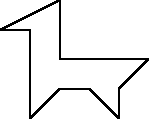
\includegraphics{../graphics/llamaPlot.pdf}\\
Louie Llama & & how we'll draw him
\end{tabular}
\]

\begin{prob} 
Here's Louie Llama hanging out near the point $0$ in the complex
plane. Multiply him by $2$. Make a table and show in the plane below what happens.  What transformation do you see?  
\[
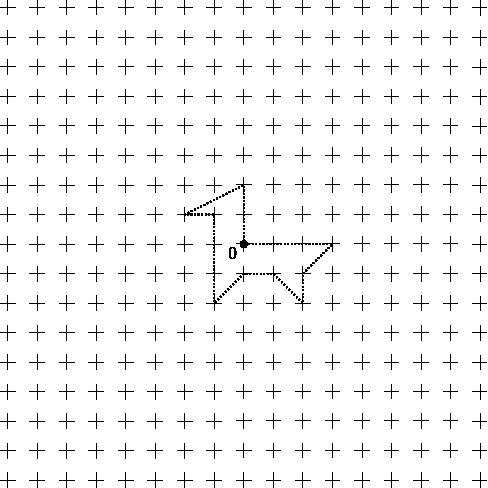
\includegraphics{../graphics/complexMult.pdf}
\]
\end{prob}

\break

\begin{prob} 
Now multiply him by $i$. Make a table and show in the plane below what happens.  What transformation do you see?  
\[

\includegraphics{../graphics/complexPlane.pdf}
\]
\end{prob}

\vfill

\begin{prob} 
Now multiply Louie Llama by $1+i$. Make a table and show in the plane
below what happens.  What transformation do you see?  
\[

\includegraphics{../graphics/complexPlane.pdf}
\]
\end{prob}

\vfill



\begin{prob} 
Now multiply Louie Llama by $\frac{1}{2}+\frac{\sqrt{3}}{2}i$. Make a
table and show in the plane below what happens.  What transformation do you see?  
\[

\includegraphics{../graphics/complexPlane.pdf}
\]
\end{prob}


\begin{prob} 
Geometrically speaking, what does it mean to ``multiply'' complex
numbers?
\end{prob}



\begin{prob}
Summarize your results from the previous problems.  
Then explain what happens when we ``multiply'' Louie Llama by a complex
number. 
\end{prob}


%\newpage
\section{To the Second Degree}\label{deg2Ext}

In this activity, we seek to understand why roots of polynomials with
real coefficients must always come in conjugate pairs.

\begin{prob}
Consider your favorite (non-real) complex number, I'll call it
$\xi$. Find a polynomial with real coefficients whose degree is as
small as possible having your number as a root. What is the degree
of your polynomial?
\end{prob}


\begin{prob}
I'll call the polynomial found in the first problem $s(x)$. Let $f(x)$
be some other polynomial with
\[
f(\xi) = 0.
\]
I claim $s(x) | f(x)$. Explain why if $s(x)\nmid f(x)$ then there exist $q(x)$ and $r(x)$ with
\[
f(x) = s(x) \cdot q(x) + r(x)\qquad\text{with }\deg(r) <\deg(s).
\]
\end{prob}

\begin{prob}
Plug in $\xi$ for $x$ in the equation above. What does this tell you
about $r(\xi)$? Is this possible?
\end{prob}

\begin{prob}
Explain why complex roots must always come in conjugate pairs. Also
plot some conjugate pairs in the complex plane and explain what
``conjugation'' means geometrically.
\end{prob}


%\newpage
\section{Undoing---Using Inverse Functions}



\begin{prob}
Formulas are fine, but what do you do to solve something like this:
\[
5 = e^x \qquad \text{}
\]
\end{prob}





and To Infinity and Beyond!)

What about equations that can't be put (or easily) put into a nice
form?  They might have solutions too, but if we only rely on the
``undoing'' means, we may never find them (and thus, all most students
are given in school are those ``rigged up'' equations- yes- important
to know how to solve, but they're not the only ones around)!  For
example, if you involve two or more types of functions in the same
equation (say exponential, log, and polynomial- e.g., $5\cdot
2^{x-4}-x^13 + \ln(x) + 102.8=0$), you now have several different
kinds of ``undoings'' to contend with.

Over the centuries, methods have been developed to deal with the
``ugly'' cases mentioned in the paragraph above.  Usually, we only end
up with an approximate answer, but we can often dictate how close the
answer can be to the actual (by analyzing the algorithms and figuring
out how many steps would be necessary to get as close as we need to
be).

\paragraph{Graphing Calculator} 
With the advent of powerful technology, we can often sidestep many of
these mathematical issues with even a simple hand-held graphing
calculator (which probably has a ``solve'' feature that will (usually)
give you a solution closest to a value you give it (if a solution
exists)).  You can also do a little more yourself by using the
graphing feature and (best done by bringing everything over = 0 and
enter the function on the other side and find its x-intercepts by
using the ``zoom'' feature).  Side question, though: How is the
calculator doing these things?  How was it programmed?  What
mathematical methods is it using?

However, you can also do a few other techniques that require a bit
more work.  For example:

\paragraph{Judicious Guess and Check}  
Don't underestimate this technique, which is the first technique that
we really should start with in early childhood (e.g., ``Fill in the
brackets: $15-\langle\, \rangle=6$''.  Before knowing any ``undoing''
techniques, we guess and check judiciously until we see that $9$ is what
makes the statement true- perhaps using objects and/or couching it in
a story problem.).  It can also lead to an expression(s) to model the
story problem if you can't already find one (perhaps it helped you in
the \textit{Dreaded Story Problem} to do just that!).  

For solving the equations that are wacky like the one above that
involved a lot of function types, we basically do the same as the
early childhood student (with a little more background) and can use
the calculator to do the grungy calculating for us.  Enter and guess
our first solution to be, say, 4 and see if that gives us zero when we
plug it in.  Unfortunately, $f(4) = -67108754.81$, which apparently is
not zero!  But we guess again and plug in, say, 1 and we get $f(1) =
102.425$.  I claim that we can guarantee that there is a solution
between $x = -1$ and $x = 4$ (why?).  Now hone in on that solution (or
maybe even find others in that interval).  We'll do the ``bisection''
technique here, which means we'll test the midpoint between $1$ and $4$
(and all midpoints of subsequent intervals): 2.5: $f(2.5) \approx -150000$. So, we have an answer between 1 and 2.5 (why?).  Try $f(1.75)=
-1339.348$.  Try 1.375 (midpoint between 1 and 1.75); $f(1.375)=41.132$,
which is greater than zero, so our answer must be between 1.375 and
1.75.  Try that midpoint: 1.5625: $f(1.5625)=-226.703<0$.  So the answer
must be between 1.375 and 1.5625: try 1.46875: $f(1.46875)=-43.9713<0$.
So we know our answer must be between 1.46875 and 1.375.  And so on
until we get the accuracy we need.  There are several variations on
this technique (in terms of how to find your next guess.  Here we
always used the midpoint).

\paragraph{Fixed Point Iteration} 
(You might look at the activity ``Spreadsheet Mania'' before embarking
on this method).  Often, when teaching algebra to students who only
know how to solve linear equations, I will find students who make an
initial stab at solving, say, a quadratic equation for $x$, in the
following manner:
\begin{align*}
x^2 + 2x -8 &= 0 & \\
2x &= 8 - x^2 & \\
x &= 4- .5 x^2 & \text{(divided by $2$)}
\end{align*}
Or, they will do something like this:
\begin{align*}
x^2 + 2x -8 &= 0 \\
x(x+2) &= 8 \\
x = \frac{8}{x+2}
\end{align*}
Of course, this seems pointless, as we don't get an equation of the
tried and true form ``x = a number''.  Instead, we get 
\[
x= \text{another expression in terms of $x$} 
\]
or ``x = g(x).'' What should we do with such students?  Suspend or
expel them???! Actually, the students are not wrong (other than not
finding a numerical answer).  These are re-writings (``interior
decorating'') of the original equation.  But what good are they?

It turns out that, under certain conditions, we can take advantage of
this form to get a solution (but not necessarily all solutions) by
using this form $g(x)=x$ and plugging in an initial value into $g(x)$
and plugging the result back into g(x), and so on.  Under certain
conditions, the values will approach a solution (i.e., we keep getting
roughly the same value over and over, meaning the $g(x)$ we're getting
is the same as the $x$ we'll plug in next, thus satisfying the
original equation).  And it's a nice method for when $x$ can be solved
for using traditional algebraic techniques (``undoing''), but just not
for a number.
      
You can use your calculator or (much quicker yet) the spreadsheet to
do this (How is this related to recursion??).
      
In our example, we already know the solutions to the equation from previous schoolwork.  That is, $x = 2$ and $x = - 4$.
\begin{enumerate}
\item Use $x=\frac{8}{x+2}$ .  Start with $x = 4$ and plug it into the right side (the initial value is often called the ``seed'').  We get $8/6= 1.\bar{3}$.  Now plug $1.\bar{3}$ into the same expression and get $2.4$.  Then plug in $2.4$ into it, etc., etc.  Keep doing this about 10 times (10 iterations) and you'll notice that the resulting values bounce before and after 2, one of our known solutions.  In fact, you'll find that no matter what your seed is (even, say, -4000), you'll relatively quickly be converging to 2.  However, no seed will get you close to the other solution (-4).  (How can this be done on a spreadsheet?: See the later activity ``Spreadsheet Mania'' for a good shortcut method to avoid the drudgery you've experienced)
\item Try the other ``solution'' we came up with in the intro:  $g(x) = 4-.5x^2$  Try it, no matter what you put in for your seed or the number of iterations, it won't get close to either solution (in fact, it sometimes will ``blow up'').  Thus, some forms are better than others for this method.
\item Say we wanted to solve $x^3 – 3x = 0$.  (We can do this
conventionally by factoring out $x$ and getting $0$, and +/- square root
of 3 (about 1.732)).  We can also ``solve for x'' and get $x = x^3 –
2x$.  Using $x^3-2x$ as our $g(x)$, use 1 as your seed and what happens?
Will any seed or \# of iterations get us reasonably close to the known
roots?  Try an alternative: $x = (1/3)x^3$. (Try seeds = 1.732, 1.735,
1.738.  What happened?  Try seed=1.7.  What happened?)  

\item Try another quadratic equation (known solutions again): $x^2+9x+19 = 0$.  Solve for $x = -19/(x+9)$ and use several seeds.  Do you get close to a solution?
Which one?  

\item Now solve an equation we have no idea about a solution
for: $x^2 – \cos(x) = 0.$  Solving for $x$ gives $x = \sqrt{\cos(x)}$.  Can you
conjecture a solution?  Check that it works in the original equation
on a calculator. 
\item When does this ``fixed point'' technique work?
Put the graphs of our $g(x)$'s with the graph $y=x$ (Why would this make
sense to do?).  Because we're not as familiar with some of the $g(x)$'s,
let's use g(x) = linear graphs first.  Use the spreadsheet as well:
Use $g(x) = 2x +3, -2x + 3, .7x + 3, 1.1x +3, .92x + 3$., etc. with
several seeds.  You'll have to fill down quite a ways (say 1000) to
see what's happening.  Sketch the graph of each with y=x and see what
happens graphically.  Make a conjecture as to when fixed point
iteration works or not.  

\item This idea of ``fixed point'' is
generalized to more powerful equation solving algorithms, including
Newton's Method.  It is generalized even more to solving other kinds
of equations, such as differential equations.
\end{enumerate}
\paragraph{Calculus-Based Techniques} For you calculus fans out there, another famous equation-solving method is ``Newton's Method''.  It's reasonably simple to understand- just need to see a picture involving tangent lines to see the reasoning. We might visit this in Math 111.


%\newpage
\section{Yet Another Division Theorem}\label{gaussianInt}


Take a minute to recall the \textit{Division Theorem}. Got it? OK we
can do something similar with complex numbers. Check this out:

\begin{definition}\index{Gaussian integers} 
A \textbf{Gaussian integer} is a number of the form
\[
a + bi
\]
where $a$ and $b$ are integers and $i$ is the square-root of negative
one.
\end{definition}

Just like with integers, we have a division theorem here too, check it
out (this time I'll play nice):

\begin{theorem}[Division Theorem]\index{Division Theorem!for Gaussian integers}
Given any Gaussian integer $\alpha$ and a nonzero Gaussian integer
$\beta$, there exist Gaussian integers $\theta$ and $\rho$ such that
\[
\alpha = \beta \cdot \theta + \rho \qquad \text{with}\qquad 
\rho\cdot\bar{\rho} <  \beta\cdot\bar{\beta}
\]
where $\bar{a + bi} = a - bi$.
\end{theorem}

Suppose you want to divide $7+7i$ by $1+2i$ and end up with quotient
and remainder that are both Gaussian integers. How do you do this?
We'll use the complex plane to help us out.
\[
\includegraphics{../graphics/complexPlane.pdf}
\]
\begin{prob} 
Mark $1+2i$ and $7 +7i$ on the complex plane. Use the grid above to
help you and be sure to label your work.
\end{prob}

\begin{prob}
Mark every Gaussian integer multiple of $1+2i$ on the plane
above. Explain what happens and explain why it happens.
\end{prob}


\begin{prob} 
Find the nearest multiple of $1+2i$ to $7+7i$.
\end{prob}

\begin{prob}
Use your work above to help find $\theta$ and $\rho$ such that
\[
7 + 7i  = (1+2i)\cdot \theta + \rho \qquad \text{with}\qquad 
\rho\cdot\bar{\rho} <  5.
\]
\end{prob}

\begin{prob}
Are the $\theta$ and $\rho$ you found above unique? Discuss.
\end{prob}

\begin{prob} 
Explain what is going on here in terms of geometry.
\end{prob}

\begin{prob}
Find $\theta$ and $\rho$ such that
\[
9 + 8i  = (5+2i)\cdot \theta + \rho \qquad \text{with}\qquad 
\rho\cdot\bar{\rho} <  29.
\]
As a gesture of friendship, I have provided a fresh grid for your
work.
\[
\includegraphics{../graphics/complexPlane.pdf}
\]
\end{prob}



\begin{prob}
Are the $\theta$ and $\rho$ you found above unique? Discuss.
\end{prob}


%\newpage
\section{Broken Records}\label{A:orderMod}

Fill in the following table:
\[
{\renewcommand{\arraystretch}{1.8}
\renewcommand{\arraycolsep}{3mm}
\begin{array}{|r||c|c|c|c|c|c|c|c|c|c|}\hline
\text{modulus:} & 2 & 3 & 4 & 5 & 6 & 7 & 8 & 9 & 10 & 11 \\ \hline\hline
2\cdot 1 \equiv & & & & & & & & & & \\ \hline
2\cdot 2 \equiv & & & & & & & & & & \\ \hline
2\cdot 3 \equiv & & & & & & & & & & \\ \hline
2\cdot 4 \equiv & & & & & & & & & & \\ \hline
2\cdot 5 \equiv & & & & & & & & & & \\ \hline
2\cdot 6 \equiv & & & & & & & & & & \\ \hline
2\cdot 7 \equiv & & & & & & & & & & \\ \hline
2\cdot 8 \equiv & & & & & & & & & & \\ \hline
2\cdot 9 \equiv & & & & & & & & & & \\ \hline
2\cdot 10\equiv & & & & & & & & & & \\ \hline
2\cdot 11\equiv & & & & & & & & & & \\ \hline
\end{array}}
\]

\begin{prob} 
Find patterns in your table above, clearly describe the patterns you find.
\end{prob}

\begin{prob} 
Consider the patterns you found. Can you explain why they happen?
\end{prob}

\begin{prob}
When does a column have a $0$? When does a column have a $1$? 
\end{prob}

\begin{prob}
Describe what would happen if you extend the table for bigger
moduli and bigger multiplicands.
\end{prob}


\vfill

\newpage


\[
{\renewcommand{\arraystretch}{1.8}
\renewcommand{\arraycolsep}{3mm}
\begin{array}{|r||c|c|c|c|c|c|c|c|c|c|}\hline
\text{modulus:} & 2 & 3 & 4 & 5 & 6 & 7 & 8 & 9 & 10 & 11 \\ \hline\hline
3\cdot 1 \equiv & & & & & & & & & & \\ \hline
3\cdot 2 \equiv & & & & & & & & & & \\ \hline
3\cdot 3 \equiv & & & & & & & & & & \\ \hline
3\cdot 4 \equiv & & & & & & & & & & \\ \hline
3\cdot 5 \equiv & & & & & & & & & & \\ \hline
3\cdot 6 \equiv & & & & & & & & & & \\ \hline
3\cdot 7 \equiv & & & & & & & & & & \\ \hline
3\cdot 8 \equiv & & & & & & & & & & \\ \hline
3\cdot 9 \equiv & & & & & & & & & & \\ \hline
3\cdot 10\equiv & & & & & & & & & & \\ \hline
3\cdot 11\equiv & & & & & & & & & & \\ \hline
\end{array}}
\]

\begin{prob} 
Find patterns in your table above, clearly describe the patterns you find.
\end{prob}

\begin{prob} 
Consider the patterns you found. Can you explain why they happen?
\end{prob}


\begin{prob}
When does a column have a $0$? When does a column have a $1$? 
\end{prob}


\begin{prob}
Can you describe what would happen if you extend the table for bigger
moduli and bigger multiplicands?
\end{prob}

\begin{prob}
Describe precisely when a column of the table will contain
representatives for each integer modulo $n$. Explain why your
description is true.
\end{prob}



%\newpage
\section{Close, but No Cigar}

Sometimes, we are not able to come up with formulas for our function
models.  In fact, sometimes all that we have are a few data points $(x,
y)$.  Obviously, we'd like to know more exact values of our function,
but the cupboard is often bare---we have to make lemonade out of
lemons.  Thus, we try to ``fill in'' points in between the given points
in order for our model to have some predictive quality to it.

You already saw this in Statistics 145 when you talked about the
``best-fit'' line.  There actually could be several definitions of what
is meant by this, but typically we use the ``least-squares'' line.
Although we usually see the formula for the slope and intercept of
this line either just quoted or derived with multi-variable calculus
in textbooks (something probably not done with the limited time
allotted for Math 111), you can actually find it for yourself using
algebraic ideas from school (although it also would be nice to know
why those algebraic ideas work!):

\begin{prob}
Find the ``least-squares'' line for the data points $(2, 3)$, $(4,
5)$, and $(6, 11)$ (note that these don't already form a line- graph
or algebraically see or just use common sense): That is, find $a$ and
$b$ so that the sum of the squares of the vertical distances of the
above data points from the line $y=ax+b$ is as small as possible
(Unpack what these words really say---a graph is probably best!  Then
solve algebraically using what you know from Algebra II or so).
\end{prob}

\begin{prob}
Of course, contrary to the ``linear disease'' that engulfs our
country, not every variable grows at the same rate all the time (i.e.,
we're not always on cruise control or, mathematically, not every
relationship is linear!)!  If the data you're given appear to be
non-linear, we try to fit a predictive non-linear curve to such a
graph (e.g., if the graph appears to be exponential in nature, we try
to fit a ``best-fit exponential function'' $y=ke^{ax}$ instead of a
``best-fit'' line $y=ax+b$).  Now how can you tell if a graph appears
to be exponential or more like a polynomial?  For example, look at the
data below:
\[
\begin{array}{|c|c|c|c|c|}\hline
x & 0 & 1 & 2 & 3 \\ \hline
y & 8.1 & 22.1 & 60.1 & 165 \\ \hline
\end{array}
\]

A group of students graph the data.  Susie says, ``This sure looks
like a parabola!''  But Fred says, ``No it doesn't, I just got done
studying exponentials and it looks like an exponential!''  Susie says
in reply, ``What?! I sat in those boring classes with you---I know
about exponentials, but I also know my parabolas---and this is a
parabola.''  Then Julie chimes in, ``Both of you dummies are wrong,
it's a quartic ($x^4$)''.  Then a whole slew of ``Says who? Says me!''
ensues.  Before this turns into a brawl and people get hurt, how can
we sanely tell who is right, if any of them? They can't all be right!


Hint: Think about the most famous graph of all, the one you know most
about.  And see if you can somehow convert the above data to get that
type of graph by graphing the relationship between variables related
to $x$ and $y$ That is, if it was truly best modeled by $y=ke^{ax}$,
then we'd know (why?) $\ln(y) = ax \ln(k)$ (try graphing the
$x$-coordinates on the horizontal axis and the natural log of the $y$
coordinates on the vertical axis. What should that graph look like if
it is best modeled by an exponential?).  If it were best modeled by $y
= kx^a$ (i.e., like a polynomial), then we'd know (why?) $\ln(y) =
a\ln(x) + \ln(k)$ (what would you graph on each axis here?).  Graph
each of these with the given data and see what happens (and find best
values for either $k$ or $a$ for the model you conjecture is best.  Note:
We could ask you to find the ``best-fit'' line for the ``linearized'' data
like in \#1, but we'll give you a break and just ask for a good eyeball
estimate here!)).

Now do the same with this data:
\[
\begin{array}{|c|c|c|c|c|}\hline
x & 1 & 2 & 3 & 4 \\ \hline
y & 8.3 & 443.6 & 24420.8 & 1364278.6 \\ \hline
\end{array}
\]

Now do the same with this data:
\[
\begin{array}{|c|c|c|c|c|c|}\hline
x & 1 & 2 & 3 & 4 & 5 \\ \hline
y & 7 & 62 & 220 & 506 & 1012 \\ \hline 
\end{array}
\]
\end{prob}

\begin{prob}
Although not all data are modeled by polynomials, because of their
easy function evaluations (place value, all K-8 arithmetic!) and
smoothness of graphs, polynomials are often a universal go-to model
for data (we try to fit a polynomial that contains all the data
points).  As was noted in Polly Nomial \#3, there are a couple of ways
to do this, at least one of which you'll do in a future activity.

Note: sometimes, finding ``best-fit'' curves can be done by a graphing
calculator (On the TI-83 and its kin, go to STATS, enter your
(2-variable) data into EDIT, and go to CALC (where you'll find LinReg,
CubicReg (cubic polynomial), ExpReg , etc.)  Of course, the
graphing calculator will blindly give you the ``best-fit'' curve of
all ilk's.  It still takes, as illustrated above, a human mind to
figure out which, if any, best fit the given data.for purposes of
prediction.
\end{prob}


\newpage
\section{On The Road}\label{A:traffic}


\begin{prob} 
Steve likes to drive the city roads. Suppose he is driving down a road
with three traffic lights. For this activity, we will ignore yellow
lights, and pretend that lights are either red or green.
\begin{enumerate}
\item How many ways could he see one red light and two green lights?
\item How many ways could he see one green light and two red lights?
\item How many ways could he see all red lights?
\end{enumerate}
\end{prob}

\begin{prob} 
Now suppose Steve is driving down a road with four traffic lights.
\begin{enumerate}
\item How many ways could he see two red light and two green lights?
\item How many ways could he see one green light and three red lights?
\item How many ways could he see all green lights?
\end{enumerate}
\end{prob}

\begin{prob} 
In the following chart let $n$ be the number of traffic
lights and $k$ be  the number of green lights seen. In each square, write the number of ways this number of green lights could be seen while Steve drives down the street.
\[
\begin{array}{|c|c|c|c|c|c|c|c|}
    \hline
          & k=0 & k=1 & k=2 & k=3 & k=4 & k=5 & k = 6\\
    \hline
    n=0 &\rule[0mm]{0mm}{7mm}&       &       &       &       &   &   \\
    \hline
    n=1 &\rule[0mm]{0mm}{7mm}  &       &       &       &       &   &   \\
    \hline
    n=2 & \rule[0mm]{0mm}{7mm} &     &     &       &       &    &  \\
    \hline
    n=3 &\rule[0mm]{0mm}{7mm}       &       &       &       &       &   &   \\
    \hline
    n=4 & \rule[0mm]{0mm}{7mm}      &       &       &       &       &   &   \\
    \hline
    n=5 &\rule[0mm]{0mm}{7mm}       &       &       &       &       &   &   \\
    \hline
    n=6 &\rule[0mm]{0mm}{7mm}       &       &       &       &       &   &   \\
    \hline
\end{array}
\]
Describe any patterns you see in your table and try to explain them in
terms of traffic lights.
\end{prob}


\newpage
\section{Pascal's Triangle: Fact or Fiction?}\label{A:factOrFiction}

\fixnote{Maybe connect to previous activity.}
Consider the numbers $\binom{n}{k}$.  These numbers can be arranged
into a ``triangle'' form that is popularly called ``Pascal's
Triangle''.  Assuming that the ``top'' entry is $\binom{0}{0}=1$, we
write the numbers row by row, with $n$ fixed for each row.  Write out
the first 7 rows of Pascal's Triangle.

\vspace{4in}


Note that there are many patterns to be found.  Your job is to justify
the following patterns in the context of relevant models. Here are three patterns, can you explain them?
\begin{enumerate}
\item $\binom{n}{k} = \binom{n}{n-k}$.
\item The sum of the entries in each row is $2^n$.
\item $\binom{n}{k-1} + \binom{n}{k} = \binom{n+1}{k}$.
\end{enumerate}



%\newpage
\section{Pascal's Pyramid}\label{A:pyramid}

A \textit{pyramid} is a three-dimensional object that has some polygon
as its base and triangles that converge to a point as its sides. Fancy
folks call a triangular-based pyramid a
\textit{tetrahedron}.\index{tetrahedron}
\[
\includegraphics[scale=.5]{../graphics/pyr.pdf}
\]
Since three-dimensional objects are hard to view on a flat sheet of
paper, sometimes we think about them by taking cross sections:
\[
\includegraphics[scale=.5]{../graphics/planeCross.pdf}
\]
We're going to build a triangular-based pyramid out of numbers. Here
are the first four cross sections:
\[
1 \qquad 
\begin{tabular}{@{\,}c@{\,}c@{\,}c@{\,}}
1 & & 1\\
 & 1 & 
\end{tabular}
\qquad 
\begin{tabular}{@{\,}c@{\,}c@{\,}c@{\,}c@{\,}c@{\,}}
1 & & 2 & & 1 \\
 & 2 & & 2 &  \\
 & & 1 & &  
\end{tabular}
\qquad
\begin{tabular}{@{\,}c@{\,}c@{\,}c@{\,}c@{\,}c@{\,}c@{\,}c@{\,}}
1 & & 3 & & 3 & & 1 \\
 & 3 & & 6 & & 3 &  \\ 
 & & 3 & & 3 & &  \\ 
 & & & 1 & & &  
\end{tabular}
\]
This pyramid that we are building is called \textbf{Pascal's
  pyramid}.\index{Pascal's!pyramid}

\begin{prob} 
Give the next two cross sections of Pascal's pyramid. Explain your
reasoning.
\end{prob}


\begin{prob} 
Do you see any connections to Pascal's Triangle in Pascal's pyramid?
Explain what you see.
\end{prob}


\begin{prob} Use the Binomial Theorem to expand:
\[
(a + x)^3
\]
\end{prob}



\begin{prob} 
Replace $x$ above with $b+c$, and use the Binomial Theorem again along
with your computation above to expand:
\[
(a + b + c)^3
\]
\end{prob}


\begin{prob} 
What do you notice about the coefficients in the expansion of $(a + b + c)^3$?
\end{prob}


\begin{prob} Explain how the trinomial coefficient
\[
\binom{n}{j,k} = \frac{n!}{j! k!(n-j-k)!}
\]
corresponds to entries of Pascal's pyramid. Feel free to draw diagrams
and give examples.
\end{prob}

\begin{prob} 
The trinomial coefficient $\binom{n}{j,k}$ has the following
``physical'' meaning: It is the number of ways one can choose $j$
objects and $k$ objects from a set of $n$ objects. Try a couple of
relevant and revealing examples to provide evidence for this claim.
\end{prob}

\begin{prob}  
Explain how Pascal's Triangle is formed. In your explanation, use the
notation $\binom{n}{j,k}$. If you were so inclined to do so, could you
state a single equation that basically encapsulates your explanation
above?
\end{prob}


\begin{prob} 
Use Pascal's pyramid to expand:
\[
(a + b + c)^4
\]
Try to formulate a ``Trinomial Theorem.''
\end{prob}

\begin{prob} Use your Trinomial Theorem to explain why the numbers in the $n$th cross section of Pascal's pyramid sum to $3^n$.
\end{prob}

%%%%%%%%%%%%%%%%%%%%%%%%%%%%%%%%%%%%%%%%%%%%
%%%%%%%%%%%%%%%%%%%%%%%%%%%%%%%%%%%%%%%%%%%%
%% REF - R. L. Keeney and James F. Ramaley
%% Mathematics Magazine, Vol. 42, No. 4 (Sep., 1969), pp. 210-213 
%%


\newpage
\section{You Can Count on It!}\label{A:countOnIt}

\fixnote{Incorporate LaTeX comments into a teaching note.}

% The words permutation and combination tend to promote formulaic thinking rather than careful reasoning.  And students tend to ask “does order matter” in ways that often don’t help them with the reasoning. 
%
%What I think they need are: (1) the multiplication principle of counting (and this gives them permutations for free, without the name); and (2) strong explanatory thinking around “n choose k,” connecting them to both traffic lights and Pascal’s triangle.  
%
%  See the final exam review document from 2014.  

%Tomorrow Delanie will aim to complete Activity A45.  These are notes about a conversation we had earlier this evening.  
%
%The major point/purpose is the fundamental counting principal and the ability to use it thoughtfully (i.e., supported by thinking) rather than formulaically.  Although we will find formulas for (n choose k) to be useful, we need not emphasize formulas for, say, permutations.
%
%We found that the activity often jumps into the deep end.  So here are some ways we decided to soften it a bit. 
%
%First, it needs a simple introduction:  
%
%A.45.0.  The Diet-Lite restaurant offers 5 entrees and 3 side dishes.   Assuming one of each, how many different dinners can you order?
%
%The primary purpose to illustrate the multiplication principle for a situation where you can draw the whole tree diagram.  The secondary purpose is to illustrate the utility of solving an easy problem before solving a hard one.  The students might find it useful in some of the later problems (e.g., 45.6 and 45.7) to solve easier problems first.  
%
%Second, two of the problems should be omitted, at least the first time through:  
%
%A.45.4. Pizza toppings is best saved until later, after the formula for (n choose k) has been firmly established.  Then it can make very useful connections. 
%
%A.45.8.  The crazy dinner orders problem is too involved for an activity.  Much better as a homework problem.  


\begin{prob}
The Diet-Lite restaurant offers 5 entrees, 8 side dishes, 12 desserts,
and 6 kinds of drinks.  If you were going to select a dinner with one
entr\'ee, one side dish, one dessert, and one drink, how many different
dinners could you order?
\end{prob}

\begin{prob}
A standard Ohio license plate consists of two letters followed by two
digits followed by two letters.  How many different standard Ohio
license plates can be made if: 
\begin{enumerate}
\item There are no more restrictions on the
numbers or letters.
\item  There are no repeats of numbers or letters.
\end{enumerate}
\end{prob}

\begin{prob}
Seven separate coins are flipped.  How many different results are
possible (e.g., HTHHTHT is different than THHHTTH)?
\end{prob}


\begin{prob}
A pizza shop always puts cheese on their pizzas.  If the shop offers
$n$ additional toppings, how many different pizzas can be ordered
(Note: A plain cheese pizza is an option)?
\end{prob}

\begin{prob}
There are 10 students in the auto mechanics club.  Elections are
coming up and the members are holding nominations for President, Vice
President, Secreatary, and Treasurer.  If all members are eligible,
how many possible tickets are there?
\end{prob}

\begin{prob}
Same as the previous question, but now there are $n$ members of the club
and $k$ offices.
\end{prob}


\begin{prob}
Now the club (with $n$ members) is not electing officers anymore, but
instead deciding to send $k$ delegates to the state auto mechanics
club convention.  How many possible groups of delegates can be made?
\end{prob}

\begin{prob}
The Pig-Out restaurant offers 5 entrees, 8 side dishes, 12 desserts,
and 6 kinds of drinks.  If you were going to select a dinner with 3
entr\'ees, 4 side dishes, 7 desserts, and one drink, how many
different dinners could you order?
\end{prob}


\newpage
\section{Which Road Should We Take?}

\begin{prob} Consider a six-sided die. Without actually rolling a die, guess the number of 1's, 2's, 3's, 4's, 5's, and 6's you would obtain in 50 rolls. Record your predictions in the chart below:
\begin{center}\textbf{Predictions}\end{center}
\[
\begin{tabular}{|c|c|c|c|c|c|c|}\hline
\# of 1's & \# of 2's & \# of 3's & \# of 4's & \# of 5's & \# of 6's & Total \\ \hline 
\rule[0mm]{0mm}{7mm} \hspace{15mm} &  \hspace{15mm} & \hspace{15mm} & \hspace{15mm} & \hspace{15mm} & \hspace{15mm} & \hspace{15mm}\\ \hline
\end{tabular}
\]


Now roll a die 50 times and record the number of 1's, 2's, 3's, 4's, 5's, and 6's you obtain.  
\begin{center}\textbf{Experimental Results}\end{center}
\[
\begin{tabular}{|c|c|c|c|c|c|c|}\hline
\# of 1's & \# of 2's & \# of 3's & \# of 4's & \# of 5's & \# of 6's & Total \\ \hline 
\rule[0mm]{0mm}{7mm} \hspace{15mm} &  \hspace{15mm} & \hspace{15mm} & \hspace{15mm} & \hspace{15mm} & \hspace{15mm} & \hspace{15mm}\\ \hline
\end{tabular}
\]
How did you come up with your predictions? How do your predictions
compare with your actual results? Now make a chart to combine your
data with that of the rest of the class.

\end{prob}

\paragraph{Experiment 1}  We investigated the results of throwing 
one die and recording what we saw (a $1$, a $2$, ..., or a $6$).  
We said that the probability of an event (for example, getting a ``3'' 
in this experiment) predicts the frequency with which we expect to see 
that event occur in a large number of trials.
You argued the $P(\text{seeing }3)=1/6$ (meaning we
expect to get a $3$ in about $1/6$ of our trials) because there were
six different outcomes, only one of them is a $3$, and you expected
each outcome to occur about the same number of times.

\paragraph{Experiment 2}
We are now investigating the results of throwing two dice and
recording the sum of the faces. We are trying to analyze the
probabilities associated with these sums.  Let's focus first on
$P(sum=2)=?$. We might have some different theories, such 
as the following:


\paragraph{Theory 1} 
$P(\text{sum}=2)=1/11$. 

It is proposed that a sum of $2$ was $1$ out
of the $11$ possible sums $\{2,3,4,5,6,7,8,9,10,11,12\}$.


\paragraph{Theory 2} 
$P(\text{sum}=2)=1/21$. 

It is proposed that a sum of $2$ was $1$ of
$21$ possible results, counting $1+3$ as the same as $3+1$:

\[
\begin{array}{cccccc}
1+1 & - & - & - & - & - \\
2+1 & 2+2 & - & - & - & - \\
3+1 & 3+2 & 3+3 & - & - & - \\
4+1 & 4+2 & 4+3 & 4+4 & - & - \\
5+1 & 5+2 & 5+3 & 5+4 & 5+5 & - \\
6+1 & 6+2 & 6+3 & 6+4 & 6+5 & 6+6 
\end{array}
\]

\begin{teachingnote}
Some might suggest that the sample space is better thought of as ordered pairs rather than sums.  In any case, the upshot is that for anything we do with the two dice, the sample space has 36 elements.  Then the following activity, Lumpy and Eddy, might be redundant.
\end{teachingnote}

\begin{prob}
Propose your own Theory 3.  
\end{prob}

%\subparagraph{Theory 3} $P(\text{sum}=2)=1/36$. 
%
%It was proposed that a
%sum of $2$ was $1$ of $36$ possible results, counting $1+3$ as
%different from $3+1$:
%\[
%\begin{array}{cccccc}
%1+1 & 1+2 & 1+3 & 1+4 & 1+5 & 1+6 \\
%2+1 & 2+2 & 2+3 & 2+4 & 2+5 & 2+6 \\
%3+1 & 3+2 & 3+3 & 3+4 & 3+5 & 3+6 \\
%4+1 & 4+2 & 4+3 & 4+4 & 4+5 & 4+6 \\
%5+1 & 5+2 & 5+3 & 5+4 & 5+5 & 5+6 \\
%6+1 & 6+2 & 6+3 & 6+4 & 6+5 & 6+6 
%\end{array}
%\]

\begin{prob}
Test all theories by computing $P(2)$, $P(3)$, \dots , $P(12)$ for each theory and comparing to the dice rolls recorded by the class.  What do you notice?  
\end{prob}

\begin{prob}
Which theory do you like best?  Why?
\end{prob}


\begin{prob}
 How could we test our theory further?
\end{prob}


\newpage
\section{Lumpy and Eddie}

Two ancient philosophers, Lumpy and Eddie, were sitting on rocks
flipping coins. 

\begin{prob} Lumpy and Eddie wondered about the probability of obtaining both a head and a tail. Here is how it went:
\begin{quote}
Eddie argued the following: ``Look Lumpy, it's clear to me that when
we flip two coins, we should get one of each about half the time
because there are two possibilities: They're either the same or
different.'' Lumpy, on the other hand, argued this way: ``Eddie, stop
being a wise guy! If we flipped two coins, we should expect both a
head and tail to come up about a third of the time because there are
only three possibilities: two heads, two tails, and one of each.''
\end{quote}
Which, if any, of these two guys is right?  Is there another answer?
\end{prob}

\begin{prob}
Next Lumpy and Eddie threw a third coin in the mix and wondered about
the probability of obtaining 2 heads and a tail or 2 tails and a head.
\begin{enumerate}
\item What would Lumpy say in this case?
\item What would Eddie say in this case?
\end{enumerate}
Be sure to clearly explain why you think they would answer in the way
you suggest.
\end{prob}



\newpage
\section{Go Climb a Tree!} 

In this activity, we'll evaluate the probabilities of complex events
using tree diagrams, fraction arithmetic, and counting.

\begin{prob}
Give a story problem that is modeled by the expression:
\[
\frac{3}{7} \times \frac{2}{5}
\]  
Let the start of the story be: ``$2/5$ of the class are girls.''  Once
you have the story, solve it using pictures (use rectangles for the
wholes) and explain why it makes sense that multiplying fractions is
the same as multiplying the numerators and multiplying the
denominators.
\end{prob}

\begin{prob}
The Weather Channel has predicted that there is a 70\% chance of rain today, a 20\% chance of rain tomorrow, and a 40\% chance of rain the day after tomorrow.  Use a tree diagram to help answer the following:
\begin{enumerate}
\item What is the probability that it will rain today and not rain tomorrow? 
\item What is the probability it will rain on exactly one of the first two days?
\item What is the probability that it will rain today, not rain tomorrow, and rain the following day?
\item What is the probability that it will rain on exactly two of the three days?
\item What is the probability it will rain on all three days?
\item What is the probability it won't rain at all?
\item What is the probability it will rain on at least one of the days?
\end{enumerate}
\end{prob}

\begin{prob}
The Indians and the Yankees are to face each other in a best-of-seven series.  The probability that the Indians will win any game is 30\%.
\begin{enumerate}
\item What is the probability that the Indians win games 1, 3, 4, and 6 to win the series?
\item What is the probability that the Indians win the series in exactly 6 games?
\item What is the probability that the Indians win the series?
\end{enumerate}
\end{prob}

\begin{prob} 
Fred the Slob has an unreliable car that starts only 65\% of the days.
If the car doesn't start, poor Fred must walk the one block to work.
This week, he is slated to work 6 days (Monday through Saturday).  
\begin{enumerate}
\item What is the probability that Fred will walk on Monday and Wednesday
and drive the other days?
\item What is the probability that Fred will
drive on exactly 4 of the days? 
\item What is the probability that poor Fred will have to walk on at least two of the days?
\end{enumerate}
\end{prob}

\begin{prob}
Use the techniques of this activity (i.e., using a special case and
fraction arithmetic to help investigate a more general case) to find
the probability of passing a 10-question multiple choice test if you
must get 70\% or more correct to pass.
\end{prob}


\newpage
\section{They'll Fall for Anything!}\label{A:fallForAnything}

What is incorrect about the following reasoning? Be specific!

\begin{prob}
Herman says that if you pick a United States citizen at random, the
probability of selecting a citizen from Indiana is because Indiana is
one of 50 equally likely states to be selected.
\end{prob}


\begin{prob}
Jerry has set up a game in which one wins a prize if he/she selects an
orange chip from a bag.  There are two bags to choose from.  One has 2
orange and 4 green chips.  The other bag has 7 orange and 7 green
chips.  Jerry argues that you have a better chance of winning by
drawing from the second bag because there are more orange chips in it.
\end{prob}

\begin{prob}
Gil the Gambler says that it is just as likely to flip 5 coins and get
exactly 3 heads as it is to flip 10 coins and get exactly 6 heads
because
\[
\frac{3}{5} = \frac{6}{10}
\]
\end{prob}

\begin{prob}
We draw 4 cards without replacement from a deck of 52.  Know-it-all
Ned says the probability of obtaining all four 7's is
$\frac{4}{\binom{52}{4}}$ because there are ways to select the
$\binom{52}{4}$ 4 cards and there are four 7's in the deck.
\end{prob} 

\begin{prob}
At a festival, Stealin' Stan gives Crazy Chris the choice of one of
three prizes---each of which was hidden behind a door.  One of the
doors has a fabulous prize behind it while the other two doors each
have a ``zonk'' (a free used tube of toothpaste, etc.).  Crazy Chris
chooses Door \#1.  Before opening that door, Stealin' Stan shows Chris
that hidden behind Door \#3 is a zonk and gives Chris the option to
keep Door \#1 or switch to Door \#2.  Chris says, ``Big deal.  It doesn't
help my chances of winning to switch or not switch.''
\end{prob}



%\newpage
\activity\section{The Harmonic Triangle}\index{harmonic triangle} 

Leibniz, one of the inventors of calculus, dreamed up this beast while
trying to solve a problem posed to him by Huygens:
\[
\begin{tabular}{@{\,}c@{\,}c@{\,}c@{\,}c@{\,}c@{\,}c@{\,}c@{\,}c@{\,}c@{\,}}
& & & & $\frac{1}{1}$ & & & & \\
& & & $\frac{1}{2}$ & & $\frac{1}{2}$ & & & \\
& & $\frac{1}{3}$ & & $\frac{1}{6}$ & & $\frac{1}{3}$ & & \\
& $\frac{1}{4}$ & & $\frac{1}{12}$ & & $\frac{1}{12}$ & & $\frac{1}{4}$ &\\
$\frac{1}{5}$ & & $\frac{1}{20}$ & & $\frac{1}{30}$ & & $\frac{1}{20}$ & & $\frac{1}{5}$
\end{tabular}
\]

\begin{prob} 
What relationships can you find between the entries of the triangle as
we move from row to row?
\end{prob}


\begin{prob} What are the next two rows? Clearly articulate how to produce more rows of the Harmonic Triangle.
\end{prob}

\begin{prob} Explain how the following expression
\[
\frac{1}{k\binom{n}{k}}
\]
corresponds to entries of the Harmonic Triangle. Feel free to draw
diagrams and give examples.
\end{prob}

\begin{prob}  
Explain how the Harmonic Triangle is formed. In your explanation, use
the notation
\[
\frac{1}{k\binom{n}{k}}
\]
If you were so inclined to do so, could you state a single equation
that basically encapsulates your explanation above?
\end{prob}

\begin{prob} 
Can you explain why the numerators of the fractions in the Harmonic
Triangle must always be $1$?
\end{prob}


\begin{prob} Explain how to use the Harmonic Triangle to go from:
\[
\frac{1}{2} + \frac{1}{6} + \frac{1}{12} + \frac{1}{20}+\cdots
\]
to
\[
\left(1 - \frac{1}{2}\right) + \left(\frac{1}{2}-\frac{1}{3}\right) + 
\left(\frac{1}{3}- \frac{1}{4}\right) + \left(\frac{1}{4}-\frac{1}{5}\right) + \cdots 
\]
Conclude by explaining why Leibniz said:
\[
\frac{1}{2} + \frac{1}{6} + \frac{1}{12} + \frac{1}{20}+\cdots = 1
\]
\end{prob}

\begin{prob} Explain how to use the Harmonic Triangle to go from:
\[
\frac{1}{3} + \frac{1}{12} + \frac{1}{30} + \frac{1}{60}+\cdots 
\]
to
\[
\left(\frac{1}{2} - \frac{1}{6}\right) + \left(\frac{1}{6}-\frac{1}{12}\right) + 
\left(\frac{1}{12}- \frac{1}{20}\right) + \left(\frac{1}{20}-\frac{1}{30}\right) + \cdots 
\]
Conclude by explaining why Leibniz said:
\[
\frac{1}{3} + \frac{1}{12} + \frac{1}{30} + \frac{1}{60}+\cdots = \frac{1}{2}
\]
\end{prob}

\begin{prob} 
Can you generalize the results above? Can you give a list of infinite
sums and conjecture what they will converge to?
\end{prob}





%%%%%%%%%%%%%%%%%%%%%%%%%%%%%%%%%%%%%%%%%%%%
%%%%%%%%%%%%%%%%%%%%%%%%%%%%%%%%%%%%%%%%%%%%
%% REF - Cut the knot
%% http://www.cut-the-knot.org/Curriculum/Combinatorics/LeibnitzTriangle.shtml
%% The Origins of the Infinitesimal Calculus. Margaret E. Baron. Dover 1969  
%%


%\newpage
\activity\section{Whoops!}


Niccol\`{o} Fontana Tartaglia was a great mathematician of the
1500's. Once he claimed claimed that the sums
\[
1+2+4, \qquad 1+2+4+8, \qquad 1+2+4+8+16, \qquad\text{and so on,} 
\]
are alternately prime and composite.

\begin{prob}
Investigate Tartaglia's claim and report your findings.
\end{prob}

One thing that would make analyzing this claim easier would be if we
had a simple formula for his sums. 

\begin{prob} 
Using a table, see if you can guess a formula for Tartaglia's sums.
\end{prob}

\begin{prob} 
Can you explain why your formula holds? Can you generalize your
formula?
\end{prob}


\begin{prob}
Expand out the following:
\begin{enumerate}
\item $(a^2 -1)(1 + a^2 + a^{2 \cdot 2})$
\item $(a^2 -1)(1 + a^2 + a^{2 \cdot 2}+a^{3 \cdot 2})$  
\item $(a^2 -1)(1 + a^2 + a^{2 \cdot 2}+a^{3 \cdot 2} + a^{4 \cdot 2})$ 
\end{enumerate}
\end{prob}

\begin{prob} Expand out the following:
\[
(2^a - 1)(1 + 2^a + 2^{2a} + 2^{3a} + \dots + 2^{(b-1)a})
\]
what does this say about Tartaglia's conjecture above?
\end{prob}




%\newpage
\activity\section{Big Primes}


All over the world, computers are churning away, trying to to find the
next prime. This is what is known as the Great Internet Mersenne Prime
Search---or (don't laugh) \index{GIMPS}GIMPS. If you are willing, you
too can play along and donate time on your computer. Every year or so
a new prime is found, and glory-everlasting\footnote{This might be a
slight exaggeration.} goes to the person who finds it! I will not
attempt to be up to date. Please use some inter-web-search-doo-hicky
or whatever to find the largest known prime. Please write the actual
number below:

\vspace{1in}

There is little doubt in my mind that this largest known prime will be
of the form:
\[
M_n = 2^n -1
\]
where $n$ is some number. Numbers of this form are
called \textit{Mersenne} numbers.\index{Mersenne numbers}

\begin{prob} 
Make a table of the Mersenne numbers $M_n$ for $n$ from $1$ to $10$. 
\end{prob}

\begin{prob} 
Which of the numbers in your table are prime? Make a conjecture.
\end{prob}

\begin{prob} 
Continue your table out to $M_{14}$. Check your conjecture up to this
point.
\end{prob}


\begin{prob} 
Compare this activity to the activity \textit{Whoops!} What do you
notice?
\end{prob}


By the way, we should add---$M_{n}$ grows very fast as $n$
grows. Let's do some comparisons:

\begin{prob} 
Which is bigger, the largest known Mersenne prime or the number of atoms
in \textit{you}?
\end{prob}

\begin{prob} 
Which is bigger, the largest known Mersenne prime or the number of
atoms in the planet Earth?
\end{prob}

\begin{prob} 
Which is bigger, the largest known Mersenne prime or the number of
atoms in the Sun?
\end{prob}

\begin{prob} 
Which is bigger, the largest known Mersenne prime or the number of
atoms in the visible Universe?
\end{prob}





%% \chapter{Enrichment Topics}

%% \newpage
\section{Continued Fractions}

We're going to use some tricks involving fractions to study numbers
that have a nasty form. As an example, consider 
\[
\sqrt{2} = 1.4142135623\dots \index{sqrt2@$\sqrt{2}$}
\]
Yuck! That's just some crazy decimal. It would be nice if we could
somehow see some order in this chaos! To do this, we'll need some
definitions:

\begin{dfn}\index{continued fraction} A fraction of the form
\[
a_0 + \frac{a_1}{\displaystyle b_1 
          + \frac{a_2}{\displaystyle b_2 
          + \frac{a_3}{\displaystyle b_3 
       + \frac{a_4}{\displaystyle b_4 + \cdots
}}}}
\]
is called a \textbf{continued fraction}. If $a_1,a_2,a_3,\dots$ are
all $1$, we will call this a \textbf{simple continued fraction}.
\end{dfn}


\begin{dfn}\index{whole-number part} 
The \textbf{whole-number part} of a number is the largest whole number
which is less than or equal to the given number.
\end{dfn}

\begin{eg} 
The whole-number part of $2$ is $2$, while the whole-number part of
$5.32$ is $5$.
\end{eg}

\begin{dfn}\index{fractional part} 
The \textbf{fractional part} of a number is the number minus its
whole-number part.
\end{dfn}

\begin{eg} 
The fractional part of $2$ is $0$, while the fractional part of $5.32$
is $0.32$.
\end{eg}


\begin{ques} 
Why don't we just describe the fractional part of a number as the part
that is to the right of the decimal point? Hint: Think about
$0.99999\dots$.
\end{ques}
\QM

Given any number, we can write it as a simple continued
fraction. Consider $13/5$. To start note that
\[
3>\frac{13}{5}>2. 
\]
So this means that 
\[
\frac{13}{5}=2 + \frac{3}{5}.
\]
Here $2$ is the whole-number part and $3/5$ is the fractional part of
$13/5$. But in the simple continued fraction, our numerator is $1$,
not $3$. How do we deal with this? Well,
\[
\frac{13}{5}=2+\frac{3}{5}=2+\frac{1}{ \frac{5}{3}}.
\]
This is an improvement but we only want whole numbers in our simple
continued fractions and not $5/3$. So we write
\[
\frac{5}{3}=1+\frac{2}{3}
\]
which gives us
\[
\frac{13}{5}=2+\frac{1}{\displaystyle 1+\frac{2}{3}}.
\]
Again, we want our numerator to be $1$, not $2$ so we will repeat the steps above to get
\[
\frac{13}{5}=2+\frac{1}{\displaystyle 1+\frac{2}{3}}=2+\frac{1}{\displaystyle 1+ \frac{1}{\frac{3}{2}}} 
=2+\frac{1}{\displaystyle 1+\frac{1}{\displaystyle 1+\frac{1}{2}}}
\]
and this last expression is the simple continued fraction for $13/5$. 
We could also list our steps as:
\begin{align*}
\frac{13}{5} & = \mathbf 2 +\frac{3}{5} \\
\frac{1}{\frac{3}{5}}  = \frac{5}{3} & = \mathbf 1 + \frac{2}{3} \\
\frac{1}{\frac{2}{3}}  = \frac{3}{2} & = \mathbf 1 + \frac{1}{2} \\
\frac{1}{\frac{1}{2}} & = \mathbf 2 +0
\end{align*}
These boldface numbers tell us our continued fraction expansion.

We can also find the simple continued fraction of numbers which are
not already fractions (otherwise this would all be a bit silly).
Consider $\sqrt{2}$, remember how yucky it was?
\[
\sqrt{2} = 1.4142135623\dots \index{sqrt2@$\sqrt{2}$}
\]
To beautify this number, note that $2>\sqrt{2}>1$. So this means that
\[
\sqrt{2} = 1 + (\sqrt{2} -1).
\]
Where $1$ is the whole-number part and $(\sqrt{2} -1)$ is the
fractional part of $\sqrt{2}$. Alright, now look at
$1/(\sqrt{2}-1)$. Again we want to separate the whole-number part and
the fractional part. With a little algebra we see that
\[
\frac{1}{\sqrt{2}-1} = \frac{\sqrt{2}+1}{2-1} = \sqrt{2}+1 =
2+(\sqrt{2}+1-2) = 2 + (\sqrt{2}-1).
\]
Now don't you get bogged down in the steps. Here it is in fast forward:
\begin{align*}
\sqrt{2} &= \mathbf{1} + (\sqrt{2} -1) \\
\frac{1}{(\sqrt{2} -1)} &= \mathbf{2} + (\sqrt{2}-1) \\
\frac{1}{(\sqrt{2} -1)} &= \mathbf{2} + (\sqrt{2}-1) \\
\frac{1}{(\sqrt{2} -1)} &= \mathbf{2} + (\sqrt{2}-1), \\
&\hspace{.5em}\vdots
\end{align*}
At each step we want:
\[
\text{number} = \text{whole-number part} + \text{fractional part}
\]
Now from the bold-faced numbers above we will make our continued fraction:
\[
\sqrt{2} = \mathbf{1} + \frac{1}{\displaystyle \mathbf{2}
          + \frac{1}{\displaystyle \mathbf{2} 
          + \frac{1}{\displaystyle \mathbf{2} 
       + \frac{1}{\displaystyle \mathbf{2} + \cdots
}}}}
\]
Beautiful!
\begin{ques} Can you explain why this works?
\end{ques}
\QM

\begin{ques} 
Do you think you could find a regular fraction equal to $\sqrt{2}$?
\end{ques}
\QM


\subsubsection{Some Hidden Beauties}

Continued fractions allow us to see patterns that are otherwise
totally hidden.

Check out $e = 2.718281828459045\dots$. \index{e@$e$}It turns out that
\[
e = 2 + \frac{1}{\displaystyle 1
          + \frac{1}{\displaystyle 2 
          + \frac{1}{\displaystyle 1 
       + \frac{1}{\displaystyle 1
          + \frac{1}{\displaystyle 4 
          + \frac{1}{\displaystyle 1 
       + \frac{1}{\displaystyle 1
          + \frac{1}{\displaystyle 6 
          + \frac{1}{\displaystyle 1 + \cdots  
}}}}}}}}}
\]

Also check out $\pi = 3.14159265358\dots$.\index{pi@$\pi$} In 1999
L.J.\ Lange found this amazing continued fraction for $\pi$:
\[
\pi = 3 + \frac{1^2}{\displaystyle 6
          + \frac{3^2}{\displaystyle 6 
          + \frac{5^2}{\displaystyle 6 
       + \frac{7^2}{\displaystyle 6 
          + \frac{9^2}{\displaystyle 6 
       + \frac{11^2}{\displaystyle 6 + \cdots
}}}}}}
\]
Wow!



\newpage

\subsection*{Problems for Section \thesection}\hrule\vspace{1ex}
\begin{enumerate}
\item Explain what the \textbf{whole-number part} and what the
  \textbf{fractional part} of a number are. Give examples.
\item Find the simple continued fraction expansion of $1/2$. Explain
  your work.
\item Find the simple continued fraction expansion of $11$. Explain
  your work.
\item Find the simple continued fraction expansion of $5/3$. Explain
  your work.
\item Find the simple continued fraction expansion of $15/11$. Explain
  your work.
\item Find the simple continued fraction expansion of $22/17$. Explain
  your work.
\item Using a calculator, find the first five terms in the simple
  continued fraction expansion of $\pi$. What number do you get by
  only considering the first term? The first four?
\item Find the simple continued fraction expansion of
  $\sqrt{5}$. Explain your work.
\item Find the simple continued fraction expansion of
  $\sqrt{10}$. Explain your work.
\item Find the simple continued fraction expansion of
  $\sqrt{17}$. Explain your work.
\item Find the simple continued fraction expansion of
  $\sqrt{26}$. Explain your work.
\item Find the simple continued fraction expansion of
\[
\frac{1 + \sqrt{5}}{2}
\]
Explain your work. Note---this is a special number, it is called the
\textit{golden ratio}. More on this later.\index{golden ratio}
\item Courtney Gibbons is someone who has a rather unusual tattoo. She
  was kind enough to let an unusual person like me take a picture of
  it.  What does her tattoo represent? Explain your reasoning.
\[
\includegraphics[width=2in]{../graphics/cgtat.pdf}
\]
\item What is it about the numbers $2,5,10,17,26$ that makes it easy
  to compute the continued fraction expansion of the square-roots of
  these numbers? Explain your answer.
\item What is the best rational approximation of $\sqrt{2}$ where the
  denominator is less than 10? Less than 20? Less than 30? Less than
  100?
\item What is the best rational approximation of $\sqrt{5}$ where the
  denominator is less than 10? Less than 20? Less than 30? Less than
  100?
\item What is the best rational approximation of $\sqrt{3}$ where the
  denominator is less than 10? Less than 20? Less than 30? Less than
  100?
\end{enumerate}



%% \newpage
\section{Tonic, Dominant, Octave}

Someone once told me ``Music is how math sounds.'' I'm not totally
sure I believe them, but maybe there is some truth to what they are
saying. Sound is made by compression waves in the air. Loosely
speaking, the closer the compression waves come, the higher the pitch
the sound is that we hear. We visualize these compression waves with a
picture like this:
\[
\includegraphics[width=3in]{../graphics/basicWave.pdf}
\]
The peaks of the waves above represent high-pressure points where the
air is very compressed, and the troughs of the waves above represent
low-pressure points, where there are very few air molecules. 

Let's call a sound produced by a single compression wave a \index{tone}
\textit{tone}. When two tones are played at the same time, their waves
act together like the sum of the individual waves. Let's
see this in action. If we play the following two tones at the same
time,
\[
\includegraphics[width=3in]{../graphics/superComb.pdf}
\]
we end up with 
\[
\includegraphics[width=3in]{../graphics/superSum.pdf}
\]
which is nothing more than every point on the first graph added to
every point on the second graph. See how when the waves line up
nicely, we get a nice big wave? See how when the waves disagree, our
wave dwindles down to nothing?

Since the time when people started making sounds, we've noticed that
some tones sound better together than others. There is an easy
rule-of-thumb that will tell you when two tones will sound ``right''
together. If the graph of both waves combined has a lot of beats \index{beats}
then it will probably sound ``wrong,'' see the example below:
\[
\begin{tabular}{ccc}
\includegraphics[width=2in]{../graphics/minorComb.pdf}
 & \raisebox{4ex}{\huge$\Rightarrow$} &
\includegraphics[width=2in]{../graphics/minorSum.pdf}\\
& & beats
\end{tabular}
\]
If the beats are hard to see, then it will sound ``right.'' You can
see this in the following example:
\[
\begin{tabular}{ccc}
\includegraphics[width=2in]{../graphics/fifthComb.pdf}
 & \raisebox{4ex}{\huge$\Rightarrow$ }&
\includegraphics[width=2in]{../graphics/fifthSum.pdf} \\
& & no beats
\end{tabular}
\]
Now let's define some words:

\begin{dfn} 
The \textbf{wavelength}\index{wavelength!sinusoidal wave} of a
sinusoidal wave is length of a complete wave, the distance from peak
to peak or the distance from trough to trough.
\end{dfn}

\begin{dfn} 
The \textbf{frequency}\index{frequency!sinusoidal wave} of a sinusoidal
wave is the number of complete waves per unit time.
\end{dfn}

If we're talking about sound waves, then wavelength and frequency are related by the following equation:
\begin{equation}\label{E:sin}
w_s \cdot f = s\qquad\text{where}\qquad
\begin{tabular}{l}
$w_s$ is the wavelength of the sound wave\\
$f$ is the frequency \\
$s$ is the speed of sound 
\end{tabular}
\end{equation}



\begin{dfn} 
The tone that you start with is called the
\textbf{tonic}.\index{tonic}
\end{dfn}

So let's start with the tonic, and add a tone whose wavelength is half
that of the tonic:
\[
\begin{tabular}{ccc}
\includegraphics[width=2in]{../graphics/octaveComb.pdf}
 & \raisebox{4ex}{\huge$\Rightarrow$ }&
\includegraphics[width=2in]{../graphics/octaveSum.pdf}
\end{tabular}
\]
That looks like it sounds really ``right,'' as there are no beats to be seen.

\begin{dfn}
The tone whose wavelength is half that of the tonic is called the
\textbf{octave}.\index{octave}
\end{dfn}

For some reason, the human ear and brain work together to identify the
tonic and octave as \textit{the same} tone, with the octave just being
twice as high. Now let's get a little crazy, we'll start with the
tonic, and add a tone whose wavelength is $2/3$ that of the tonic:
\[
\begin{tabular}{ccc}
\includegraphics[width=2in]{../graphics/fifthComb.pdf}
 & \raisebox{4ex}{\huge$\Rightarrow$ }&
\includegraphics[width=2in]{../graphics/fifthSum.pdf}
\end{tabular}
\]
That looks like it sounds ``right'' too, no beats again.

\begin{dfn}
The tone whose wavelength is $2/3$ that of the tonic is called the
\textbf{dominant}.\index{dominant}
\end{dfn}

The dominant is central to all of western music. The
tonic-dominant-octave trio of tones is sometimes called a \textit{power
  chord} for its powerful sound.

\begin{ques}
Starting with just these three notions: Tonic, dominant, and octave
what tones would we want an instrument to be able to play?
\end{ques}
\QM

We seek the answer to this question.

\subsection{Instrument Building}

Close your eyes, and imagine you are on a beach in Brazil, imagine
yourself swimming in the gentle waves. While you are swimming, you
decide that when you return to your home town you are finally going to
build that stringed instrument that you've always wanted---perhaps a
lytherette. You'd have to pick some frequency for the open
string. OK---done.


\begin{ques} What do waves look like on your stringed instrument?
\end{ques}

Let me explain a somewhat sticky point. The waves made by strings on
instruments are not nice old sinusoidal waves, they are what we call
\textit{standing waves}\index{standing waves}. Standing waves look
like a vibrating string:
\[
\includegraphics[width=3in]{../graphics/stand.pdf}
\]
Notice how the string is attached at the dots on the left and right?
Points like those are called \textit{nodes}\index{nodes}. While there
are many places that nodes can be, for us nodes will always be at the
endpoints of the string.

\begin{dfn} 
The \textbf{wavelength}\index{wavelength!standing wave} of a standing
wave is twice the length from node to node.
\end{dfn}

\begin{dfn} 
The \textbf{frequency}\index{frequency!standing wave} of a standing
wave is the number of complete vibrations (up and down) per unit time.
\end{dfn}

If we're talking about strings on instruments, then wavelength and
frequency are related by the following equation:
\begin{equation}\label{E:standing}
w_t \cdot f = c\qquad\text{where}\qquad
\begin{tabular}{l}
$w_t$ is the wavelength of the standing wave \\
$f$ is the frequency \\
\begin{minipage}{30ex}$c$ is a constant based on the mass and tension of the string\end{minipage}
\end{tabular}
\end{equation}

\begin{ques} 
If you pluck a string, what will the wavelength of the sound wave be?
Use equations (\ref{E:sin}) and (\ref{E:standing}) to express your
answer in terms of $w_t$, $f$, $c$ and $s$.
\end{ques}
\QM


\begin{ques} 
If you shorten a string's length by one-third, what will the
wavelength of the new sound wave be?  Use equations (\ref{E:sin}) and
(\ref{E:standing}) to express your answer in terms of $w_t$, $f$, $c$
and $s$.
\end{ques}
\QM

The upshot of the two questions above is that if you want to produce a
tone whose wavelength is a fraction of another tone's wavelength, then
your merely pluck a string whose length is the same fraction of the
string that produced the original tone. Let's get back to instrument building.

\begin{ques} 
When building a musical instrument, what tones do you want to be able
to play?
\end{ques}

I'll take this one! You want to be able to play tonic (open string),
the dominant, and the octave. How do we make this happen? Let's
imagine we are building a stringed instrument. Many stringed
instruments use \textit{frets}\index{frets} (little metal things that
help make new tones) to get the desired tones. To start, we'll want to
put a fret $2/3$ along the length of the string:
\[
\includegraphics[width=3in]{../graphics/dom1.pdf}
\]
Additionally, we want to be able to play the dominant of this new tone
as well. To do this, we'll might place a new fret
\[
\frac{2}{3}\cdot \frac{2}{3} = \frac{4}{9}
\]
of the length of the string. 
\[
\includegraphics[width=3in]{../graphics/pdom2.pdf}
\]
Hmmmm there is a slight problem though. This new fret would create a
note \textit{higher} than the octave ($1/2$ the length of the
string). We want all of our frets to be placed between the original
tonic and octave. So let's move this fret over by lowering our new
tone by an octave. The new wavelength will be twice as long, so we'll
put a fret $8/9$ along the length of the string.
\[
\includegraphics[width=3in]{../graphics/dom2.pdf}
\]
Now repeat this process, adding a new fret for the dominant of the
previously added tone, at each step ensuring that the fret be placed
between $1/2$ and complete string length. Do this $12$ times, let's
see what happens. Fill in the fractions in the boxes below---as a
gesture of friendship, I've given you the correct decimal approximation
for each fraction:
\[
\begin{array}{|r|c|c|c|c|c|c|}\hline
\text{fraction} &\rule[0mm]{0mm}{7mm}            &            &            &            &            &            \\ \hline
\bigstrut[t]\text{decimal}  & 0.666\dots & 0.888\dots & 0.592\dots & 0.790\dots & 0.526\dots & 0.702\dots \\ \hline
\end{array}
\]
\[
\begin{array}{|r|c|c|c|c|c|c|}\hline
\text{fraction}  &\rule[0mm]{0mm}{7mm}           &            &            &            &            &            \\ \hline
\bigstrut[t]\text{decimal}   & 0.936\dots & 0.624\dots & 0.832\dots & 0.554\dots & 0.739\dots & 0.493\dots \\ \hline
\end{array}
\]
From this we find we should place a twelfth fret $0.493\dots$ along
the length of the string. To the human ear, this tone will sound quite
close to the octave of our starting tone (though slightly
lower). Hence after twelve steps we \textit{appear} to be at the
octave. If we were to put frets on our instrument at all of these
divisions, we would have something like this:
\begin{equation}\label{E:fboard}
\begin{array}{c}
\includegraphics{../graphics/fboard1.pdf}
\end{array}
\end{equation}
Remember though, the twelfth fret is close to an octave, but not
perfect!  Mathematically we might say
\[
\frac{2^n}{3^m} \approx \frac{1}{2}
\]
for some integers $n$ and $m$. We note that in our case $m = 12$ and
$n$ is some other integer. Could we find integers $n$ and $m$ such that
\[
\frac{2^n}{3^m} =\frac{1}{2}?
\]
If so then we could write:
\[
2^{n+1} = 3^m \qquad\Leftrightarrow\qquad 2^{(n+1)/m} = 3
\]
\begin{ques}\index{Unique Factorization Theorem} 
What does the Unique Factorization Theorem for integers say about the
above expressions? How do we proceed from here?
\end{ques}
\QM 



\newpage

\subsection*{Problems for Section \thesection}\hrule\vspace{1ex}
\begin{enumerate}
\item Explain what the octave of a given tone is.
\item Explain what the dominant of given tone is.
%%
%% \item sketch the octave of a given tone!
%%
\item Order the following wavelengths by which tone they produce from
  lowest to highest.
\begin{align*}
&0.666\dots, 0.888\dots, 0.592\dots, 0.790\dots, 0.526\dots, 0.702\dots, \\
&0.936\dots, 0.624\dots, 0.832\dots, 0.554\dots, 0.739\dots, 0.493\dots
\end{align*}
Explain your reasoning.
\item Do the following tones sound ``right'' or ``wrong'' when played together?
\[
\begin{tabular}{ccc}
\includegraphics[width=2in]{../graphics/octaveComb.pdf}
 & \raisebox{4ex}{\huge$\Rightarrow$ }&
\includegraphics[width=2in]{../graphics/octaveSum.pdf}
\end{tabular}
\]
Explain your reasoning.
\item Do the following tones sound ``right'' or ``wrong'' when played together?
\[
\begin{tabular}{ccc}
\includegraphics[width=2in]{../graphics/fifthComb.pdf}
 & \raisebox{4ex}{\huge$\Rightarrow$ }&
\includegraphics[width=2in]{../graphics/fifthSum.pdf}
\end{tabular}
\]
Explain your reasoning.
\item Do the following tones sound ``right'' or ``wrong'' when played together?
\[
\begin{tabular}{ccc}
\includegraphics[width=2in]{../graphics/minorComb.pdf}
 & \raisebox{4ex}{\huge$\Rightarrow$ }&
\includegraphics[width=2in]{../graphics/minorSum.pdf}
\end{tabular}
\]
Explain your reasoning.
\item Do the following tones sound ``right'' or ``wrong'' when played together?
\[
\begin{tabular}{ccc}
\includegraphics[width=2in]{../graphics/p2Comb.pdf}
 & \raisebox{4ex}{\huge$\Rightarrow$ }&
\includegraphics[width=2in]{../graphics/p2Sum.pdf}
\end{tabular}
\]
Explain your reasoning.
\item Do the following tones sound ``right'' or ``wrong'' when played together?
\[
\begin{tabular}{ccc}
\includegraphics[width=2in]{../graphics/p1Comb.pdf}
 & \raisebox{4ex}{\huge$\Rightarrow$ }&
\includegraphics[width=2in]{../graphics/p1Sum.pdf}
\end{tabular}
\]
Explain your reasoning.
\item What is the wavelength of the dominant over the tone of
  wavelength $2/3$? Explain your reasoning.
\item What is the wavelength of the dominant over the tone of
  wavelength $3/4$? Explain your reasoning.
\item What is the wavelength of the dominant over the tone of
  wavelength $7/8$? Explain your reasoning.
\item What is the wavelength of the dominant over the tone of
  wavelength $6/13$? Explain your reasoning.
\item What is the wavelength of the dominant over the tone of
  wavelength $7/13$? Explain your reasoning.
\item What is the wavelength of the dominant over the tone of
  wavelength $2/3$ if we insist that the resulting wavelength is
  between $1/2$ and $1$? Explain your reasoning.
\item What is the wavelength of the dominant over the tone of
  wavelength $4/7$ if we insist that the resulting wavelength is
  between $1/2$ and $1$? Explain your reasoning.
\item What is the wavelength of the dominant over the tone of
  wavelength $5/8$ if we insist that the resulting wavelength is
  between $1/2$ and $1$? Explain your reasoning.
\item What is the wavelength of the dominant over the tone of
  wavelength $5/9$ if we insist that the resulting wavelength is
  between $1/2$ and $1$? Explain your reasoning.
\item What is the wavelength of the dominant over the tone of
  wavelength $6/11$ if we insist that the resulting wavelength is
  between $1/2$ and $1$? Explain your reasoning.
\item Give a precise derivation of how we obtained the fret positions
\begin{align*}
&0.666\dots, 0.888\dots, 0.592\dots, 0.790\dots, 0.526\dots, 0.702\dots, \\
&0.936\dots, 0.624\dots, 0.832\dots, 0.554\dots, 0.739\dots, 0.493\dots
\end{align*}
using the ideas of the tonic and dominant.

\end{enumerate}




\newpage


\section{Rational and Irrational Temperament}



In the last section, we were thinking about how to build a stringed
instrument with frets. With this in mind, we came up with the
following equation
\[
2^{\frac{n+1}{m}} = 3
\]
where $m$ is the number of divisions of the string that we would wish
to make. Armed with the Unique Factorization Theorem for
integers,\index{Unique Factorization Theorem} we could (and you will!)
explain that there is no rational solution of
\[
2^x = 3,
\]
meaning that  finding appropriate values of $n$ and $m$ is
actually impossible! It's a good thing that we are not the type of
people to be deterred by the impossible. In light of our discussion
above, we want to find a fraction:
\[
\frac{n+1}{m} \approx \log_2(3) = 1.58496250072115618145373894394\dots
\]

\begin{ques} 
How do we find good fractional approximations of irrational numbers?
\end{ques}

In two words: Continued fractions.\index{continued fraction} Set:
\[
x_1 = 1.58496250072115618145373894394\dots
\]
Write $x$ in terms of its whole-number part and its fractional part:
\[
x_1 = \mathbf{1} + (x_1-1)
\]
Now look at the reciprocal of $(x_1-1)$:
\begin{align*}
x_2 &=\frac{1}{x_1-1} = 1.70951129135145477697619026217\dots\\
x_2 &= \mathbf{1} + (x_2-1)
\end{align*}
Continue on:
\begin{align*}
x_3 &=\frac{1}{x_2-1} = 1.40942083965320900458240433081\dots\\
x_3 &= \mathbf{1} + (x_3-1)
\end{align*}
Again, again!
\begin{align*}
x_4 &=\frac{1}{x_3-1} = 2.44247459618085927548717403238\dots\\
x_4 &= \mathbf{2} + (x_4-2)
\end{align*}
One last time:
\begin{align*}
x_5 &=\frac{1}{x_4-2} = 2.26001675267082453593127612260\dots\\
x_5 &= \mathbf{2} + (x_5-2)
\end{align*}
Whew, now I'm tired, we could continue on but I think it is time to
stop. Let's see what our continued fraction looks like:
\[
\log_2(3) \approx 1 + \dfrac{1}{1+\dfrac{1}{1 + \dfrac{1}{2 + \dfrac{1}{2}}}}
\]
If we simplify this continued fraction into a regular old fraction we find:
\[
\log_2(3) \approx \frac{19}{12} = 1.58333333333\dots
\]
Check this out:
\[
2^{19/12} = 2.9966141537\dots
\]
This is really close to $3$, thus $2^{19/12}$ is a good approximation
of $\log_2(3)$. Write
\begin{align*}
3&\approx 2^{19/12} \\
\frac{2}{3} &\approx \frac{2}{2^{19/12}} \\
&\approx \frac{1}{2^{7/12}}
\end{align*}




With this in mind, we will adopt the convention that
the $n$th tone above the tonic will have a wavelength of exactly
$1/2^{n/12}$ of the tonic:
\[
\includegraphics[width=3in]{../graphics/firstFret.pdf}
\]
In particular, since 
\[
\frac{1}{2^{1/12}} \cdot \frac{1}{2^{1/12}} = \frac{1}{2^{2/12}}
\]
if we work with wavelengths of $1/2^{n/12}$ of the tonic, we will
obtain a nice approximation of every tone we produced before. After
$7$ steps,
\[
\frac{1}{2^{7/12}} = 0.66741992\dots \approx \frac{2}{3}
\]
and additionally, 
\[
\frac{1}{2^{12/12}} = \frac{1}{2},
\]
so after twelve steps we are exactly at the octave! If we put a frets
at the points $\frac{1}{2^{n/12}}$ letting $n$ run from $0$ to $12$, we'll obtain a picture like:
\[
\includegraphics{../graphics/eqFret.pdf}
\]
Let's compare this to our fret positions in diagram~(\ref{E:fboard}):
\[
\includegraphics{../graphics/bFret.pdf}
\]
\begin{ques} Will this really work?
\end{ques}
\QM

\subsection{Equal Temperament}

Spacing the division of the tones by making use of wavelengths that
are $\frac{1}{2^{1/12}}$ of the tonic is called \textbf{equal
  temperament}\index{equal temperament}. This is how modern guitars
and pianos are tuned. People have also identified other ratios of the
wavelength of the tonic that they thought sounded ``right.''
Essentially, they have taken the idea that we should have as few
``beats'' as possible to the extreme. When they do this, and attempt
to have $12$ tones, they arrive at what is called \textbf{just
  intonation}\index{just intonation}. When \textit{a
  cappella}\index{\textit{a cappella}@acappella} groups sing and form
chords, they usually sing using just intonation---the human brain
seems to be somehow drawn to these sounds. Here are the ratios of the
wavelength of the tonic used in just intonation:
\begin{align*}
&1/2,\quad 8/15,\quad 5/9,\quad 3/5,\quad 5/8,\quad 2/3,\\
&32/45,\quad 3/4,\quad 4/5,\quad 5/6,\quad 8/9,\quad 24/25
\end{align*}
Let's compare these to the ratios used in equal temperament:
\[
\begin{tabular}{rr@{\,}c@{\,}lr@{\,}c@{\,}l}
Tone & \multicolumn{3}{c}{Equal Temperament}   & \multicolumn{3}{c}{Just Intonation}   \\ \hline
\bigstrut[t] $12$ & $1/2^{12/12}$ & $=$ & $0.5$         & $1/2$   & $=$& $0.5$      \\
$11$ & $1/2^{11/12}$ & $=$ & $0.529\dots$  & $8/15$  & $=$& $0.533\dots$ \\
$10$ & $1/2^{10/12}$ & $=$ & $0.561\dots$  & $5/9$   & $=$& $0.555\dots$    \\
$9$  & $1/2^{9/12}$  & $=$ & $0.594\dots$  & $3/5$   & $=$& $0.6$ \\
$8$  & $1/2^{8/12}$  & $=$ & $0.629\dots$  & $5/8$   & $=$& $0.625$ \\
$7$  & $1/2^{7/12}$  & $=$ & $0.667\dots$  & $2/3$   & $=$& $0.666\dots$ \\
$6$  & $1/2^{6/12}$  & $=$ & $0.707\dots$  & $32/45$ & $=$& $0.711\dots$ \\
$5$  & $1/2^{5/12}$  & $=$ & $0.749\dots$  & $3/4$   & $=$& $0.75$ \\
$4$  & $1/2^{4/12}$  & $=$ & $0.793\dots$  & $4/5$   & $=$& $0.8$ \\
$3$  & $1/2^{3/12}$  & $=$ & $0.840\dots$  & $5/6$   & $=$& $0.833\dots$ \\
$2$  & $1/2^{2/12}$  & $=$ & $0.890\dots$  & $8/9$   & $=$& $0.888\dots$ \\
$1$  & $1/2^{1/12}$  & $=$ & $0.943\dots$  & $24/25$ & $=$& $0.96\dots$ \\ \hline
\end{tabular}
\]
The real issue with just intonation comes with we try to raise every
note up by a given number of steps. Suppose a singer has trouble
singing in the range of some song, yet has no problems if we raise
every note of the song up by $1$ half step. If our instrument is in
equal temperament, then this shift of tones will have no adverse
effects. However, if our instrument is in just intonation, then check
out what happens:
\begin{itemize}
\item Let $24/25$ of a wavelength be the new tonic---this is 1 half
  step.
\item Now $7$ steps up will be $5/8$ of a wavelength.
\end{itemize}
Checking out the new ratio we find:
\[
\frac{5/8}{24/25} = 0.651042 
\]  
This is over a $2 \%$ difference from $2/3$ of the tonic. Believe it
or not, this will be noticeably ``wrong'' to the human ear. With
equal temperament, the tone will still be spot-on.

These issues with musical instruments arise due to intrinsic
differences between rational and irrational numbers. The tones that
sound best to our ears are all defined by ratios of the wavelength of
the tonic. However, moving up by these ratios is done via
multiplication, and hence logarithms enter the scene. The Unique
Factorization Theorem for integers\index{Unique Factorization Theorem}
tells us that the ratios that we are most interested in cannot be
obtained simply from the other ratios we are interested in. From all
this arises a fascinating problem that everyone experiences without
even realizing it!


\newpage

\subsection*{Problems for Section \thesection}\hrule\vspace{1ex}
\begin{enumerate}
\item Explain why $\log_2(3)$ is an irrational number.
\item Explain why $\log_3(5)$ is an irrational number.
\item Explain why $\log_3(6)$ is an irrational number.
\item Explain why $\log_4(6)$ is an irrational number.
\item Explain why $\log_9(10)$ is an irrational number.
\item Find the simple continued fraction expansion of $5/3$. Explain
  your reasoning.
\item Find the simple continued fraction expansion of $15/11$. Explain
  your reasoning.
\item Find the simple continued fraction expansion of $22/17$. Explain
  your reasoning.
\item Using a calculator, find the first five terms in the simple
  continued fraction expansion of $e$. What number do you get by only
  considering the first term? The first two terms? The first three
  terms? The first four? The first five?  Explain your reasoning.
\item Using a calculator, find the first five terms in the simple
  continued fraction expansion of $\pi$. What number do you get by
  only considering the first term? The first two terms? The first
  three terms? The first four? The first five?  Explain your
  reasoning.
\item Suppose you are building a stringed instrument. If the first
  octave of $12$ tones has a length of $16$ inches, how long is the
  next octave? What about the next octave? Explain your reasoning.
\item A singer and a piano are playing a chord involving the sixth
  tone. If the singer is singing in just intonation, and the piano is
  in equal temperament, does the singer believe that the piano is
  playing too high or too low? Explain your reasoning.
\item A singer and a piano are playing a chord involving the seventh
  tone. If the singer is singing in just intonation, and the piano is
  in equal temperament, does the singer believe that the piano is
  playing too high or too low? Explain your reasoning.
\item A singer and a piano are playing a chord involving the fourth
  tone. If the singer is singing in just intonation, and the piano is
  in equal temperament, does the singer believe that the piano is
  playing too high or too low? Explain your reasoning.
\item A singer and a piano are playing a chord involving the twelfth
  tone. If the singer is singing in just intonation, and the piano is
  in equal temperament, does the singer believe that the piano is
  playing too high or too low? Explain your reasoning.
\item Some other cultures place $5$ tones between octaves. Can you
  explain this if you know that they are trying to approximate
  $\log_2(3)$?
\item Light also has wave-like properties. The wavelengths of the
  visible spectrum goes from around $380$ nm to $750$ nm. Sometimes
  colors are depicted as being in a line, other times they are
  depicted as being in a wheel. Can you use our discussion on music,
  thinking about tonics and octaves to give a plausible resolution to
  this paradox?

%\item The tone whose wavelength is $3/4$ that of the tonic is called
%  the \textbf{sub-dominant}.\index{sub-dominant} If we try to base a
%  tuning system on this tone, we end up trying to approximate
%  $\log_3{4}$. Can you explain why when people did this, they arrived
%  at a $19$ tone system?


%4/3 sub-dominant
%5:4 mediant
\end{enumerate}




%%%% Index and References


\addcontentsline{toc}{chapter}{References and Further Reading}


\begin{fullwidth}

\begin{thebibliography}{99}

\bibitem{averbach} B.\ Averbach and O.\ Chein. \emph{Problem Solving Through Recreational Mathematics}. Dover, 2000.

\bibitem{bag} A.K.\ Bag. \emph{Binomial Theorem in Ancient India}. Indian Journal of History of Science, vol.\ 1,  1966 68--74. 

\bibitem{baron} M.\ Baron. \emph{The Origins of the Infinitesimal Calculus}. Dover, 1987.

\bibitem{beckman} S.\ Beckmann. \emph{Mathematics for Elementary
  Teachers}. Addison Wesley, 2007.

\bibitem{bogomolny} A.\ Bogomolny. Leibniz and Pascal Triangles. \emph{Interactive Mathematics Miscellany and Puzzles}.
\\ \texttt{http://www.cut-the-knot.org/}

\bibitem{boyer} C.B.\ Boyer and U.C.\ Merzbach. \emph{A History of Mathematics}. Wiley, 1991.

\bibitem{colebrooke} H.\ Colebrooke. \emph{Classics of Indian Mathematics}. 
Sharada Publishing House, 2005.

\bibitem{dudley} U.\ Dudley. \emph{Elementary Number Theory}. Dover,
  2008.

\bibitem{dull} R.W.\ Dull. \emph{Mathematics for Engineers}. Second
  Edition. McGraw-Hill, 1941.

\bibitem{dunnMcConnell} 
E.\ Dunne and M.\ McConnell. \emph{Pianos and Continued
Fractions}. Mathematics Magazine, vol.\ 72, no.\ 2 (1999), 104-115.

\bibitem{euclid} Euclid and T.L.\ Heath. \emph{The Thirteen Books of Euclid's Elements: Volumes 1, 2, and 3}. Dover, 1956. 

\bibitem{eves} H.\ Eves. \emph{An Introduction to the History of Mathematics}. Saunders College Publishing, 1990.

\bibitem{gardner} M.\ Gardner. \emph{My Best Mathematical and Logic
  Puzzles}. Dover, 1994.

\bibitem{lange} L.J.\ Lange. \emph{An Elegant Continued Fraction for {$\pi$}}. The American Mathematical Monthly, vol. 106, no. 5, (1999), pp. 456--458.

\bibitem{livio} M.\ Livio. \emph{The Equation that Couldn't be
  Solved}. Simon\&Schuster, 2005.

\bibitem{keeneyRamaley} R.L.\ Keeney and J.F.\ Ramaley. \emph{On the Trinomial Coefficients}. Mathematics Magazine, vol. 42, no. 4 (Sep., 1969), pp. 210-213.

\bibitem{knuth} D.E.\ Knuth. \emph{The Art of Computer Programming. Volume 1: Fundamental Algorithms}. Addison-Wesley, 1975.

\bibitem{mira} J.A.\ Mira. \emph{Mathematical Teasers}. Barnes\&Noble, 1970.

\bibitem{nrich} NRICH website.
\\ \texttt{http://nrich.maths.org/}

\bibitem{papick} I.\ Papick. \emph{Algebra Connections: Mathematics
  for Middle School Teachers.} Pearson, 2007.

\bibitem{petkovic} M.\ Petkovi\'{c}. \emph{Famous Puzzles of Great Mathematicians}. American Mathematical Society, 2009.

\bibitem{polya} G.\ Polya. \emph{Mathematical Discovery: On
  Understanding, Learning, and Teaching Problem Solving.} Wiley, 1981.

\bibitem{posamentier} A.\ Posamentier. \emph{Teaching Secondary Mathematics}. Prentice-Hall, 2002.

\bibitem{tahan} M.\ Tahan. \emph{The Man Who Counted: A Collection of Mathematical Adven-
tures}. W.W.\ Norton\&Company, 1993.

\bibitem{solomon} R.\ Solomon. \emph{Abstract Algebra}. Brooks/Cole, 2003.

\bibitem{wylie} C.R.\ Wylie Jr. \emph{101 Puzzles in Thought and
  Logic}. Dover, 1957.

\bibitem{youse} B.K.\ Youse. \emph{Arithmetic: A Modern Approach}. Prentice-Hall, 1963.


\end{thebibliography}
\end{fullwidth}


%\cleardoublepage
%
\addcontentsline{toc}{chapter}{Index}
\printindex


%%%%

\end{document}
